\documentclass[twoside=false,fontsize=12pt,DIV=12,BCOR=0pt]{scrbook}
%\includeonly{turing}
\usepackage[utf8]{inputenc}
\usepackage[croatian]{babel}
\usepackage{csquotes}
\MakeOuterQuote{"}
\usepackage{amsmath,amssymb,amsthm}
\usepackage{thmtools}
\usepackage{stmaryrd}
\usepackage[unicode]{hyperref}
\usepackage[euler-digits]{eulervm}
\usepackage{beton}
\renewcommand{\bfdefault}{sbc}
%\usepackage{concmath}
%\usepackage[final]{microtype}
\usepackage{xcolor}
\hypersetup{
    colorlinks,
    linkcolor={red!50!black},
    citecolor={blue!50!black},
    urlcolor={blue!80!black}
}
\usepackage[backend=bibtex]{biblatex}
\addbibresource{literatura.bib}
\usepackage{mathtools}

\declaretheorem[style=definition,qed=$\vartriangleleft$,parent=chapter]{definicija}
\declaretheorem[sibling=definicija]{propozicija}
\declaretheorem[sibling=definicija]{korolar}
\declaretheorem[sibling=definicija]{lema}
\declaretheorem[sibling=definicija]{teorem}
\declaretheorem[sibling=definicija,style=definition,qed=$\vartriangleleft$]{primjer}
\declaretheorem[sibling=definicija,style=definition,qed=$\vartriangleleft$]{napomena}

%\usepackage{dsfont}
\usepackage{mathbbol}
\usepackage[defaultlines=3,all]{nowidow}
\usepackage{textcomp}
\usepackage{tikz}
\usetikzlibrary{automata, positioning, arrows}
\tikzset{->,>=stealth',
node distance=3cm,
%every state/.style={thick, fill=gray!10},
initial text=$ $}

\newcommand{\N}{{\mathbb N}}
%\newcommand{\f}{\mathbold}
\newcommand{\f}{\mathsf}
\newcommand{\dom}[1]{\mathcal D_{#1}}
\newcommand{\im}[1]{\mathcal I_{#1}}
\newcommand{\graf}[1]{\mathcal G_{#1}}
\newcommand{\reg}[1]{\mathcal R_{#1}}
\newcommand{\inc}{\textsc{inc}}
\newcommand{\dec}{\textsc{dec}}
\newcommand{\goto}{\textsc{go\,to}}
\newcommand{\incr}[1]{\inc\;\reg{#1}}
\newcommand{\decr}[2]{\dec\;\reg{#1},#2}
\newcommand{\remove}[2]{\textsc{remove}\;\reg{#1}\;\textsc{to}\;\reg{#2}}
\newcommand{\move}[3]{\textsc{move}\;\reg{#1}\;\textsc{to}\;\reg{#2}\;\textsc{using}\;\reg{#3}}
\newcommand{\pr}{\mathbin{\raisebox{1pt}{\textsc{\scriptsize{p\!r}}}}}
\newcommand{\kompl}{\sp{\textup{\textsf c}}}
\newcommand{\bl}{\t\textvisiblespace}

\newenvironment{prog}{\left[\begin{array}{r@{\;}l}}{\end{array}\right]}

\DeclareMathOperator{\card}{card}
\DeclareTextFontCommand{\t}{\ttfamily\upshape}

\DeclarePairedDelimiter{\knk}{\lVert}{\rVert}
\DeclarePairedDelimiter{\kins}{\ulcorner}{\urcorner}
\DeclarePairedDelimiter{\kprog}{\ulcorner}{\lrcorner}
\DeclarePairedDelimiter{\kf}{\t{\char`\{}}{\t{\char`\}}}
\DeclarePairedDelimiter{\kr}{\langle}{\rangle}


\begin{document}
\title{Izra\v{c}unljivost za računarce}
\author{Vedran Čačić}
\date{2019}
\maketitle

\tableofcontents

%\part{Modeli izračunljivosti}
\chapter{Predgovor}

%\section{Neka vrst predgovora}

Već nekoliko godina držim, na Matematičkom odsjeku Prirodoslovno-matematičkog fakulteta u Zagrebu, kolegij Izračunljivost. Taj kolegij je izvorno uveden kao prirodni nastavak kolegija Matematička logika (čijim je dijelom dugo bio), s ciljem dokaza Churchovog teorema o neodlučivosti logike prvog reda. Tako je nastala knjiga~\cite{skr:Vuk}, izdvajanjem iz knjige~\cite{skr:VukML}, koja je bila prvenstveno namijenjena studentima teorijske matematike koji žele produbiti svoje znanje o matematičkoj logici.

U međuvremenu, zbog raznih okolnosti, kolegij su počeli upisivati mahom studenti računarstva, kojima pojam algoritma predstavlja puno općenitiji i intuitivno bliži pojam od onog potrebnog da bi se dokazao Churchov teorem. U suvremenom svijetu okruženi smo računalima raznih vrsta, često ih programiramo da bismo ih prilagodili svojim potrebama, i algoritamske sustave više ne doživljavamo kao nešto apstraktno. Pojam izračunljive funkcije (funkcije implementirane u nekom programskom jeziku) počeo je već u umovima studenata računarstva istiskivati skupovnoteorijsku ideju uređene trojke $(\text{domena},\text{kodomena},\text{graf})$ kao asocijaciju na pojam "funkcija". Rekurzija više nije egzotična matematička konstrukcija, već sasvim uobičajen alat u repertoaru gotovo svakog programera. Jezici više nisu reprezentirani črčkarijama na papiru ili otiscima na traci (kao što su bili u Turingovo vrijeme), već tekstnim datotekama, nizovima bajtova u određenom \emph{encodingu}, koji se sasvim prirodno obrađuju programskim alatima. Strukture više nisu dijagrami matematičkih simbola povezanih strelicama, nego memorijski blokovi objekata povezanih pokazivačima ili referencama. \emph{Halting problem} nije više nešto maglovito i daleko od svakodnevnog iskustva: ta svi smo doživjeli da se računalo privremeno smrzne, i bili u nedoumici koliko dugo čekati prije nego što dobijemo nekakav odziv, ili zaključimo da se permanentno smrznulo i ne preostaje nam drugo doli posegnuti za gumbom za ponovo pokretanje. 

U tom svjetlu, počeli su se pokazivati određeni nedostaci knjige~\cite{skr:Vuk}. Zahvaljujući njenom pokušaju da izgradi matematičku intuiciju, potpuno zaboravljajući ili čak namjerno potiskujući intuiciju koju računarci već imaju o tim pojmovima, konačni učinak za većinu studenata bio je vrlo sličan onom koji je primijetio Eric Mazur~\cite{mazur} u svojoj nastavi fizike:
\begin{quote}
    \emph{Professor, how should I answer these questions: according to what you taught me, or according to the way I usually think about these things?}
\end{quote}

Nažalost, znao sam i ja dobivati takva pitanja. Ili sam jednostavno uočio da studenti pri programiranju koriste jedan mentalni model, a pri rješavanju zadataka sasvim drugačiji. I naravno, pritom čine puno više početničkih pogrešaka --- jer taj drugi model izgrađuju tek nekoliko mjeseci, dok prvi izgrađuju desetak godina.

Ova knjiga pokušaj je ispravljanja tog dojma. \textbf{Ne postoje dva svijeta}, svijet modernog računarstva i svijet klasične teorije izračunljivosti. To je jedan te isti svijet, samo što je u matematičkom modelu pojednostavljen (slično kao i model njutnovske mehanike: vakuum, linearno trenje, materijalne točke,~\ldots) --- ali svi bitni pojmovi teorijskog računarstva se u njemu mogu modelirati, svaka intuicija se može validirati, i svaki fenomen se može uočiti. Ako ste "računarac u duši", sve potrebne ideje već imate. I najvažnije, sistematizacija i razumijevanje koje iz toga proizlaze su nezamjenjivi.

Što ako \emph{niste} računarac u duši? Knjiga~\cite{skr:Vuk} je fantastična za izgradnju matematičke intuicije. Praktički jedini njen nedostatak je invalidacija računarske intuicije --- ako tu intuiciju nemate, nedostatka nema. Izuzetno sam se trudio održati \emph{backward compatibility}, tako da čak možete neke pojmove naučiti otamo, a neke odavdje.

\section{O knjizi}

Iako je knjigu sasvim moguće isprintati na papir i šarati po njoj, prvenstveno je namijenjena digitalnom čitanju. Zato ima puno referenci (označenih posebnom bojom), na svaku od kojih je moguće kliknuti da bi se vidjelo na što se odnosi. Ako koristite "pravi" PDF-čitač (za razliku od ovih što dođu s \emph{browserima}), možete se i vratiti tipkom \keys{\!$\Mapsfrom$}, ili kombinacijom \keys{Alt+\arrowkeyleft}. Pravi čitač omogućuje vam i navigaciju kroz naslove, bolji \emph{rendering}, označavanje omiljenih stranica i još neke stvari zbog kojih se svakako isplati instalirati ga. Moja preporuka je \textsf{SumatraPDF} na Windowsima, \textsf{Okular} na Linuxu, te \textsf{Document Viewer} na Androidu. Naravno, ako imate dovoljno RAM-a, \textsf{Adobe Reader} je također opcija. Ako baš morate čitati u internetskom pregledniku, čujem da \textsf{Firefox} ima relativno dobar \emph{plugin}.

Knjiga je pisana u \textsf{\LaTeX{}}u, klasa \textsf{KOMA-Script book}, koristeći internetsku uslugu \emph{Overleaf} koja je vjerojatno najbolji besplatni način za produkciju visoko zahtjevnih dokumenata "u oblaku". Font je Knuthov Concrete iz serije \emph{Concrete Mathematics}, a za matematiku Zapfov \AmS{} $Euler$. Ako vas zanima išta detaljnije o produkciji knjige, možete mi pisati na \href{mailto:veky@math.hr}{veky@math.hr} --- ili pogledati u (ne sasvim ažuran) repozitorij na \href{https://github.com/vedgar/izr}{github.com/vedgar/izr}. Naravno, ako uočite bilo kakvu grešku u knjizi, ili smatrate da bi nešto trebalo drugačije prezentirati, pošaljite \emph{email} ili \emph{pull request}.

Duljina knjige prvenstveno je posljedica moje želje da gotovo sve dokaze raspišem do sitnih detalja, kako bih sebi i vama pokazao da ništa nije provučeno "ispod stola", te da biste uočili da osnovnih ideja zapravo nema puno. Ogroman broj dokaza provodi se matematičkom indukcijom, rastavom na slučajeve, ili pak eksplicitnom konstrukcijom (\emph{programiranjem}) objekata koji zadovoljavaju traženu specifikaciju. Ako vam se bilo koji dokaz učini prelaganim (ili preteškim), ne morate ga čitati --- ali tako se izlažete riziku da propustite uočiti sličnu ideju u nekom idućem dokazu. Drugi uzrok veličine knjige je velik broj primjera. Vjerojatno najčešći prijedlog studenata za poboljšanje nastave na evaluacijskim anketama bio je da stavim više primjera. Čuo sam vas, i nadam se da je ovo dovoljno --- ako nije, recite.

Sastavni dio ove knjige je i Zbirka zadataka, u kojoj se nalaze brojni zadaci, od šablonskih za vježbu, preko svih zadataka sa starih kolokvija i pismenih ispita do kojih sam uspio doći (pri čemu zahvaljujem Zvonku Iljazoviću i Marku Doki --- bivšim asistentima iz Izračunljivosti --- na ustupanju zadataka), pa do zadataka koji na određeni način nadopunjuju teoriju izloženu u ovoj knjizi, ali nisu nužni za njeno razumijevanje.

Nadimak ove knjige --- \emph{Computonomicon} --- relativno je doslovni prijevod njene svrhe: prikaz ({\textgreekfont\textepsilon\textiota\textkappa\'o\textnu\textalpha}) zakona (\textnu\'o\textmugreek\textomikron\textvarsigma) računanja (\textsc{compvtvs}). Miješanje grčkih i latinskih korijena je omiljena razonoda računaraca --- promotrite pridjev "heksadecimalni".

Zahvalan sam kolegama i studentima koji su čitali rane \emph{draftove} ove knjige, i brojnim prijedlozima pridonijeli njenom poboljšanju. Među njima svakako bih istaknuo Marka Horvata, koji još uvijek nije uvjeren da je računarac, ali je pristao igrati tu ulogu za potrebe čitanja ove knjige.

\section{Motivacija}

Izračunljivost: matematička obrada pojma algoritma. Čemu to služi? Zar ne znamo pisati algoritme i bez matematičke formalizacije? Koga je zapravo briga za definicije poput "Algoritam je uređena sedmorka, čiji elementi su skupovi~\ldots", i beskorisne propozicije poput "Postoji algoritam za sortiranje liste brojeva"? Dva su moguća odgovora na to pitanje: praktični i teorijski.

Kažemo da znamo pisati algoritme. Ali kako to činimo? Zapravo ih najčešće \emph{implementiramo} u nekom programskom jeziku, prešutno podrazumijevajući da je ono što taj jezik omogućava izraziti, ni više ni manje nego algoritam. S tim shvaćanjem postoje dva problema. Prvo, programski jezici nastaju godišnjim ritmom, a jezik koji postane toliko popularan da se u njemu počnu pisati općeniti algoritmi, nastane možda svakih desetak godina. Zatrpani smo knjigama koje objašnjavaju besmrtne algoritamske koncepte, pokušavajući nam ih "približiti" implementirajući ih u jeziku koji je odavno mrtav. Neke od tih knjiga su toliko popularne da su autori gotovo primorani pisati nova izdanja, u kojima su algoritmi potpuno isti, ali je programski jezik promijenjen. Tu se krije implicitna pretpostavka da, što god jedan programski jezik može izraziti, može i drugi. No kako možemo biti sigurni u to? Na primjer, originalni FORTRAN nije dopuštao rekurziju, dok ALGOL jest~\cite{url:recursionAlgol}. Znamo li da se svaki rekurzivni algoritam može zapisati nerekurzivno? Možemo li to dokazati? Također, ako jest tako, zašto cijelo vrijeme stvaramo nove jezike? Razuman odgovor je da se razlikuju u \emph{nečem drugom}, ne u algoritmima koje prezentiraju. Možemo li "to drugo" eliminirati, svodeći algoritme samo na "čistu esenciju"?

Drugi problem sastoji se u tome da programski jezici nastaju s raznim svrhama, ali izuzetno rijetko s primarnom svrhom modeliranja matematičkih objekata. Još rjeđe takvi jezici postanu planetarno popularni. Popularni jezici su obično opterećeni performansama: optimalnom upotrebom procesora (vremena) i memorije (prostora), i kao posljedica toga njihov dizajn čini razne ustupke hardveru, koji se teško mogu matematički opravdati. Izuzetno je česta pojava, na primjer, da cijele brojeve računala ne reprezentiraju kao elemente skupa $\mathbb Z$, već kao elemente skupa $\mathbb Z\big\slash2^{64}\mathbb Z$. Također, često se instrukcije ne izvršavaju redom kojim se nalaze u izvornom kodu, u svrhu bržeg izvršavanja na višejezgrenim procesorima. Tako nastaje raskorak između algoritma i implementacije, koji ima važne praktične posljedice~\cite{url:wrongBinsearch}.

Teorijski odgovor na motivacijsko pitanje dobijemo kad se zapitamo što, u općenitom smislu, matematičare navede na formalizaciju nekog pojma. Ponekad je to otkriće paradoksa, ali češće se radi o potrebi da se dokaže \emph{nepostojanje} objekta neke klase $\mathcal K$ s nekim svojstvima. Iako smo se za dokaze postojanja mogli osloniti na intuitivni osjećaj da objekte klase $\mathcal K$ "prepoznamo kad ih vidimo", to nam očito više nije dovoljno ako slutimo da traženi objekt ne postoji, i želimo to dokazati. A u svakom se području s vremenom pojave problemi koji odolijevaju svim poznatim metodama, i počne se vjerovati da su možda nerješivi.

Dok nitko nije dovodio u pitanje Euklidove konstrukcije, puno je preciznija formulacija geometrijske konstruktibilnosti bila potrebna da se dokaže da je trisekcija kuta ravnalom i šestarom nemoguća. Dok je za pronalazak Cardanove ili Ferrarijeve formule bilo dovoljno znati nekoliko jednostavnih algebarskih manipulacija, tek je Galoisova teorija omogućila dokaz da analogni postupci nisu mogući za algebarske jednadžbe petog i višeg stupnja. Dok je već Galileo vidio da prirodnih brojeva i njihovih kvadrata ima jednako mnogo koristeći intuitivni pojam bijekcije, bitno je stroža formulacija bila potrebna Cantoru za dijagonalni argument kojim je dokazao da bijekcija između $\N$ i $\mathbb R$ ne postoji. Na meta-razini također: Cantor je uspio naći dokaze za mnoge tvrdnje ili njihove negacije u svojoj teoriji skupova, ali tek je formalna aksiomatizacija omogućila da se dokaže da takvi dokazi za neke tvrdnje (kao što je hipoteza kontinuuma), niti za njihove negacije, jednostavno ne postoje.

Od davnina je poznat problem rješavanja \emph{diofantskih jednadžbi} --- nalaženja prirodnih brojeva koji zajedno s još nekim fiksnim prirodnim brojevima, zbrajanjem i množenjem, čine dva izraza jednakima. Modernim jezikom, zadan je polinom s cjelobrojnim koeficijentima u $k$ varijabli (recimo $x_2^3-x_1^2-1$), i želimo ustanoviti ima li nultočku u $\N^k$ --- ili u $\mathbb Z^k$, što se može svesti na prirodni slučaj. Za mnoge specijalne polinome znali smo odgovor, za mnoge specijalne potklase (recimo kad je broj varijabli $k$, ili stupanj polinoma, jednak $1$) poznavali smo od davnina algoritme za nalaženje nultočaka, ali opći algoritam, koji bi za svaki takav polinom u konačno mnogo koraka odgovarao na pitanje ima li prirodnu nultočku, nismo imali. Na slavnoj Hilbertovoj listi od 23 velika matematička problema, deseti je pronalazak takvog algoritma. Protokom vremena, iskristalizirala se mogućnost da algoritam ne postoji, ali za pravi dokaz toga trebalo je prvo formalizirati pojam algoritma. Nakon što je to učinjeno, relativno brzo (uzevši u obzir da su diofantske jednadžbe bile poznate tisućama godina) je riješen i deseti Hilbertov problem --- naravno, dokazom nepostojanja takvog algoritma.

Nije to bio jedini takav problem: nađeni su brojni drugi problemi za koje se sličnim metodama dokazalo da su algoritamski nerješivi. Danas znamo da je neizračunljivost "posvuda", i nismo njome više toliko fascinirani, ali to je samo znak ogromnog puta koji smo prešli u shvaćanju algoritama tijekom dvadesetog stoljeća. Jedan dio tog puta prikazan je u ovoj knjizi.

\section{Opća i univerzalna izračunljivost}

Jedan od velikih ciljeva teorije izračunljivosti je pokazati da pojam izračunljive funkcije zapravo ne ovisi o podlozi na kojoj se njen algoritam izvršava. Iako je lako naći prejednostavne sustave (kao što su na primjer konačni automati, koji ne mogu čak niti uspoređivati proizvoljno velike prirodne brojeve), nakon neke točke dovoljne kompleksnosti svi mehanički sustavi postaju \emph{ekvivalentni} po pitanju toga koje funkcije, uz razumno kodiranje njihovih ulaza i izlaza, računaju. To se vidi iz činjenice da je svaki od njih sposoban \emph{simulirati} sve druge, odnosno reprezentirati njihove konfiguracije (ili barem njihove kodove) unutar svojih, i izvršavati korake njihovog računanja kao (možda komplicirane) procedure na svojim konfiguracijama. Suvremeno računarstvo poznaje taj fenomen pod imenom "virtualizacija". \emph{Church--\!Turingova teza} ide i dalje: kaže da se ne samo svi algoritmi izvršivi na svim formalnim modelima izračunljivosti, već i svi "intuitivno zamislivi" algoritmi, mogu izvršavati na nekom konkretnom modelu izračunljivosti, primjerice na Turingovom stroju. Tu tezu je očito nemoguće formalno dokazati --- sve dok se ne dogovorimo oko općih aksioma izračunljivosti~\cite{dershowitz} --- ali svaki dokaz ekvivalencije sustava izračunljivosti pruža dodatnu empirijsku potvrdu za nju.

Drugim riječima, izračunljivost je \emph{opći} fenomen: u kojem god modelu da je definiramo, ona će obuhvatiti iste funkcije --- ili bar iste s obzirom na prirodno kodiranje ulaza i izlaza. Na primjer, algoritmi za zbrajanje dekadski zapisanih i binarno zapisanih prirodnih brojeva očito su različiti, ali jednako tako je očito da su oba zapravo samo reprezentacije brojevne funkcije $\f{add}^2$, s obzirom na različite zapise (dekadski odnosno binarni) samih prirodnih brojeva.

Također, jedan od tih modela (pa onda i svi ostali, putem simulacije) zapravo posjeduje svojstvo \emph{univerzalnosti}: ne samo da je za svaku izračunljivu funkciju moguće naći algoritam unutar tog modela, već je moguće naći \emph{jedan} algoritam koji, ovisno o ulazima, može računati \emph{sve} izračunljive funkcije, odnosno može simulirati sve ostale algoritme. Štoviše, ta "granica dovoljne kompleksnosti", na kojoj se postiže opća izračunljivost i univerzalnost, je za neke modele začuđujuće nisko. Promotrit ćemo tri vrste takvih sustava: RAM-strojeve, Turingove strojeve, te parcijalno rekurzivne funkcije.

\section{Pregled po poglavljima}
Ovdje slijedi grubi prikaz rezultata obrađenih u pojedinom poglavlju knjige. Za više detalja pogledajte sadržaj.

U prvom poglavlju uvodimo brojevni model izračunavanja (računanje funkcija koje rade s prirodnim brojevima), kroz imperativno programiranje --- RAM-strojeve i makro-strojeve u stilu Shoenfielda~\cite{shoenfield}. Opisujemo tehniku spljoštenja (\emph{inlining}) kojom se makro-program može pretvoriti u ekvivalentni RAM-program.

U drugom poglavlju dajemo alternativni brojevni model, kroz funkcijsko programiranje --- rekurzivne funkcije u stilu Kleeneja. Koristeći funkcijski makro i spljoštenje, konstruiramo kompajler parcijalno rekurzivnih funkcija u RAM-programe, pokazujući da imperativna paradigma može simulirati funkcijsku (računajući iste funkcije).

U trećem poglavlju uvodimo kodiranje, pomoću kojeg možemo u brojevnom modelu računati i funkcije na objektima koji nisu prirodni brojevi. Koristeći kodiranje, konstruiramo interpreter RAM-programa u funkcijskom jeziku, pokazujući ekvivalentnost imperativne i funkcijske paradigme (Kleenejev teorem o normalnoj formi).

U četvrtom poglavlju uvodimo jezični model izračunavanja (računanje funkcija koje rade s nizovima znakova), kroz Turingove strojeve u stilu Sipsera~\cite{sipser}. Opisujemo Turing-izračunavanje parcijalno rekurzivnim funkcijama i transpiliramo RAM-strojeve u Turingove strojeve, čime dokazujemo ekvivalentnost brojevne i jezične izračunljivosti.

U petom poglavlju generaliziramo dobivene rezultate ekvivalentnosti raznih modela izračunavanja kroz Church--\!Turingovu tezu, te napokon dokazujemo rezultate o nepostojanju algoritma za pojedine probleme, kao što je Churchov teorem o neodlučivosti logike prvog reda. Skiciramo kako se iz toga može dobiti G\"odelov prvi teorem nepotpunosti.

U šestom poglavlju dokazujemo četiri velika teorema o metaprogramiranju: teorem o parametru (specijalni slučaj spljoštenja), teorem rekurzije (simuliranje općih rekurzija), teorem o fiksnoj točki (izračunljiva transformacija RAM-programa ne mijenja semantiku nekoga od njih) i Riceov teorem (semantička svojstva RAM-programa nisu odlučiva).

U sedmom poglavlju uvodimo rekurzivnu prebrojivost kao formalizaciju poluodlučivosti, te je karakteriziramo na razne načine kako u brojevnom tako i u jezičnom modelu: kao projekcije rekurzivnih relacija, kao čekanje na zaustavljanje izračunavanja, kao enumeracije (slike rekurzivnih nizova) i kao grafove parcijalno rekurzivnih funkcija.

\chapter{RAM-izračunljivost}

\section{Pojam izračunljive funkcije}

Da bismo odgovorili na pitanje što je algoritam, zapitajmo se za početak što algoritam \emph{radi}  --- ili, što mi algoritmom radimo. Algoritam možemo \emph{pokrenuti} na nekim \emph{ulaznim podacima}, izvršavati njegove \emph{korake} preciznim \emph{redom} te, u nekom trenutku kad algoritam to zatraži, \emph{zaustaviti} postupak i dobiti \emph{izlazne podatke}. Algoritam, u tom pogledu, obavlja nekakvu \emph{transformaciju} podataka. Štoviše, algoritam bi trebao biti \emph{deterministički}: isti ulazni podaci trebali bi proizvesti iste izlazne podatke. Matematička formalizacija te transformacije je pojam \emph{funkcije}: algoritam \emph{preslikava} ulazne podatke u izlazne. Kažemo da algoritam \emph{računa} funkciju, i takve funkcije (za koje imamo algoritme) zovemo \emph{izračunljivima}. Tako pitanje "Kakvi su algoritmi mogući?" postaje nešto preciznije pitanje "Koje su funkcije izračunljive?".

% \subsection{Vrste i količina podataka}

Da bismo funkciju mogli matematički zapisati, moramo precizirati domenu i kodomenu. \emph{Što} su naši podaci?
Na prvi pogled, mogu biti bilo što: imamo algoritme koji rade na cijelim brojevima, realnim brojevima (preciznije, njihovim aproksimacijama --- vidjet ćemo zašto je to bitno), tekstnim podacima (\emph{strings}), datotekama, mrežnim vezama (\emph{sockets}), drugim algoritmima (\emph{higher order programming}), grafovima, objektima, regularnim izrazima, i tko zna čemu. No iskustvo programiranja nas uči da se svi ti raznorazni \emph{tipovi} podataka uvijek mogu --- i moraju, ako želimo nešto raditi s njima --- reprezentirati u memoriji računala kao neki binarni podaci: konačni nizovi nula i jedinica.

Dakle, mogli bismo uzeti $\{0,1\}^*:=\bigcup_{k\in\mathbb N}\,\{0,1\}^k\nomenclature{$S^*$}{skup konačnih nizova elemenata iz $S$}$ kao univerzalni skup naših podataka --- ali pokazuje se da je zgodnije ako umjesto $\{0,1\}$ uzmemo proizvoljni konačni neprazni skup ("abecedu") $\Sigma$. Funkcije iz $\Sigma^*$ u $\Sigma^*$ zovemo \emph{jezične funkcije}, i to je povijesno bio prvi pokušaj formalizacije algoritma: Turingov stroj, kojim ćemo se baviti u poglavlju~\ref{ch:Turing}.

Ipak, skup $\{0,1\}^*$, kao i općeniti $\Sigma^*$, matematički je nespretan; recimo, ako hoćemo nešto o njemu dokazati indukcijom, moramo u koraku posebno razmatrati dodavanje nule, a posebno dodavanje jedinice. Ako hoćemo napraviti neku petlju kroz njega, nije baš lako odrediti sljedbenika zadanog elementa. Nezgoda je i u tome što uobičajenim leksikografskim uređajem nije dobro uređen: na primjer, skup $\{0^n1\mid n\in\N\}$ nema najmanji element.

Za dokazivanje teorema bolje je uzeti jednostavniji skup --- u najvećem dijelu knjige promatrat ćemo \emph{brojevne} algoritme, kojima su ulazni i izlazni podaci \textbf{prirodni brojevi}. U nekom smislu, skup prirodnih brojeva je najjednostavniji mogući skup na kojem se može obrađivati teorija izračunljivosti --- svakako je najjednostavniji među beskonačnim skupovima, a izračunljivost na konačnim skupovima je trivijalna: algoritam za svaku funkciju se može napisati kao tablica (\emph{lookup table}).

Odabir skupa $\N$ kao osnovnog isplatit će se kroz jednostavnost mnogih dokaza (jer imamo matematičku indukciju, jasan početak i sljedbenika, dobar uređaj,~\ldots), ali s druge strane, zato će biti kompliciranije \emph{kodirati} razne druge matematičke objekte kao prirodne brojeve. Za usporedbu, skup $\Sigma^*$ je zgodniji za kodiranje, jer već imamo intuitivnu predodžbu raznih objekata kao nizova znakova ($\Sigma=$ ASCII\@): nitko nam ne mora objasniti kodiranje da bismo znali koji element od $\mathbb Q$ predstavlja "\t{-22/3}".

Ipak, neintuitivnost kodiranja nadomjestit će jednostavnost algoritama: dok je, uz odgovarajuće tehnike~\cite{posav}, lako napisati algoritam za npr.\ zbrajanje racionalnih brojeva kodiranih prirodnim brojevima, analogni algoritam za ASCII-kodirane razlomke gotovo nikada ne stigne dalje od grubog pseudokoda. Ponegdje, gdje su naši objekti već \emph{definirani} kao nizovi znakova (najvažniji primjer su formule logike prvog reda), koristit ćemo njihovu jezičnu reprezentaciju, ali to će biti nakon što objasnimo općenito kodiranje sa $\Sigma^*$ na $\N$ (i obrnuto).

Smatramo li nulu prirodnim brojem? Treba li brojenje početi od $0$ ili od $1$, dilema je stara koliko i samo računarstvo~\cite{note:EWD831}. Kao i drugdje u matematici, postoje dobri razlozi za obje opcije. Zato ćemo koristiti oba skupa, no kako će nam češće trebati nula među prirodnim brojevima (pogledajte na primjer definiciju od $\{0,1\}^*$), skup s nulom imat će kraću oznaku.
\begin{align}
    %\SwapAboveDisplaySkip
	\N&:=\{\mspace{2mu}0,1,2,3,\dotsc\}\nomenclature{$\N$}{skup prirodnih brojeva s nulom}\\
	\N_+&:=\{\mspace{2mu}1,2,3,4,\dotsc\}\nomenclature{$\N_+$}{skup pozitivnih prirodnih brojeva (bez nule)}
\end{align}

%\subsection{Broj izlaznih i ulaznih podataka}\label{sec:briup}

\begin{napomena}[{name=[samo jedan izlazni podatak]}]\label{nap:brip}
Govorili smo o izlaznim podacima u množini, no s obzirom na to da nas samo zanima postojanje algoritma, ništa ne gubimo fiksiranjem broja izlaznih podataka na $1$. Algoritam s $k$ ulaznih i $l$ izlaznih podataka uvijek možemo promatrati kao $l$ algoritama s istih $k$ ulaznih podataka i s po jednim izlaznim podatkom.

    Na primjer, u nekim programskim jezicima postoji operacija $\texttt{divmod}$ iz $\mathbb Z^2$ u $\mathbb Z^2$, koja provodi dijeljenje s ostatkom u $\mathbb Z$, vraćajući količnik i ostatak. Nju uvijek možemo, ako je nemamo kao osnovnu, emulirati pomoću dvije operacije, $\div$ i $\bmod$, koje vraćaju količnik i ostatak istog dijeljenja zasebno. Razlog zašto neki jezici imaju $\texttt{divmod}$ kao posebnu funkciju leži u tome da algoritmi za te dvije operacije imaju mnogo zajedničkih koraka --- ako smo odredili količnik, obično možemo iz postupka kojim smo to učinili pročitati i ostatak (sjetite se npr.\ algoritma za dijeljenje višeznamenkastih brojeva). Zato bismo ponovnim provođenjem algoritma ispočetka za ostatak nepotrebno duplicirali korake. No ako nas samo zanima koje su funkcije izračunljive, očito postoji algoritam za $\texttt{divmod}$ ako i samo ako postoje algoritmi za \emph{koordinatne funkcije} $\div$ i $\bmod$, pa nam je dovoljno baviti se pitanjem jesu li $\div$ i $\bmod$ izračunljive --- u ovom slučaju, dakako, jesu.
\end{napomena}

Kad promatramo broj \emph{ulaznih} podataka (tzv.\ \emph{mjesnost}) algoritma, situacija je bitno drugačija. Jasno je da algoritam za npr.\ potenciranje prirodnih brojeva prima bazu i eksponent kao dva ulazna podatka, i ne može se jednostavno zapisati pomoću algoritama koji primaju po jedan ulazni podatak. %Doduše, korištenjem tehnike \emph{currying}, svaku izračunljivu funkciju možemo računati pomoću algoritama koji primaju po \emph{dva} ulazna podatka, i neki autori doista ograničavaju mjesnost na $2$, ali to stvara dosta tehničkih problema za minimalni dobitak.
Zato ćemo promatrati algoritme proizvoljnih mjesnosti $k\in\N_+$, i smatrati da mjesnost čini bitni dio identiteta algoritma. Primjerice, "zbroji 2 broja" i "zbroji 5 brojeva" su različiti algoritmi, štoviše ovaj prvi se pojavljuje kao korak (nekoliko puta) u ovom drugom.

Direktna posljedica toga je da u našem modelu ne postoje algoritmi s "varijabilnim brojem" ulaznih podataka, što je u računarstvu poznato pod nazivom \emph{varargs}. Na nekoliko mjesta gdje nam budu potrebni, modelirat ćemo ih pomoću familije algoritama svih mogućih mjesnosti --- recimo zbrajanje kao $\f{add}^k,k\in\N_+$. Mjesnost\nomenclature{$\f f^k$}{brojevna funkcija mjesnosti $k$} algoritma ili funkcije ćemo obično pisati u superskriptu ako je želimo naglasiti --- neće dolaziti do zabune s eksponentima jer ni algoritme ni funkcije nećemo potencirati, niti s oznakom $f^{-1}$ za inverznu funkciju jer mjesnost ne može biti negativna.

Iako mjesnost smatramo neodvojivim dijelom funkcije odnosno algoritma, u slučaju nespecificirane mjesnosti $k$ nespretno je pisati $x_1,x_2,\dotsc,x_k$ kad god trebamo napisati argumente odnosno ulazne podatke. Zato ćemo često tih $k$ prirodnih brojeva skraćeno pisati $\vec x$\nomenclature{$\vec x$}{nekoliko argumenata čija su imena oblika $x_1$,~\dots,~$x_k$}, ili $\vec x^k$ ako želimo naglasiti koliko ih ima --- no najčešće će se to moći zaključiti iz konteksta: recimo, u $f^7(\vec x,y,z)$, vidimo da je duljina od $\vec x$ jednaka $5$.

\begin{napomena}[{name=[svi argumenti moraju biti eksplicitno navedeni]}]\label{nap:blokovi}
S obzirom na to da promatramo samo determinističke algoritme, naglasimo da nema "implicitnih argumenata": sve vrijednosti o kojima ovisi izlaz funkcije (ako se doista mijenjaju od poziva do poziva) moraju biti prenesene u nju kao argumenti. Često ćemo pisati opće funkcijske pozive kao $f(\vec x,y,z)$, gdje su $y$ i $z$ "pravi" argumenti s kojima doista nešto radimo u konkretnom algoritmu, a $\vec x$ predstavlja samo kontekst (\hspace{-1pt}\emph{environment}) nekog vanjskog algoritma koji je pozvao $f$ --- koji također moramo prenijeti u $f$ ako želimo da mu ona može pristupiti.
\end{napomena}

Pažljiv čitatelj će primijetiti da zahtijevamo da mjesnost bude pozitivna, odnosno ne promatramo algoritme s $0$ ulaznih podataka. Ovo nije bitna restrikcija (možete se zabaviti pokušavajući otkriti koje sve tehničke detalje u knjizi treba promijeniti da bismo uključili i takve algoritme u razmatranje), ali pojednostavljuje izlaganje, a takvi algoritmi nam nisu zanimljivi iz perspektive izračunljivosti: iz napomene~\ref{nap:blokovi} slijedi da nul-mjesni algoritmi mogu računati jedino konstante, a ne treba nam jako napredni formalizam da bismo zaključili da konstante \emph{jesu} izračunljive.

\subsection{Parcijalnost}

Gdje god je dosad bilo govora o općenitim izračunljivim funkcijama, namjerno je upotrijebljen prijedlog "iz": funkcija \emph{iz} $A$ u $B$. Općenito u matematici, takva fraza označava \emph{parcijalne} funkcije, koje ne moraju biti definirane u svim točkama od $A$ (precizno, domena im je podskup od $A$). Recimo, tangens je parcijalna funkcija iz $\mathbb R$ u $\mathbb R$, jer je $\frac{\pi}{2}\in\mathbb R\setminus \dom{\text{tg}}$. Takve funkcije označavamo oznakom $f:A\rightharpoonup B$, za razliku od \emph{totalnih} funkcija koje označavamo $f:A\to B$ i zovemo ih funkcije \emph{sa} $A$ u $B$. 

Dopuštajući algoritmima da računaju parcijalne funkcije, zapravo im omogućavamo da je za neke ulazne podatke njihov rad sasvim dobro definiran (dakle, ovdje ne mislimo na izuzetke, \emph{exceptions}, kao što je dijeljenje nulom), ali da ipak ne postoji završna konfiguracija iz koje bismo mogli pročitati izlazni podatak. Nakon malo razmišljanja dolazimo do zaključka da je to jedino moguće tako da algoritam za neke ulaze beskonačno radi, odnosno nikada ne stane.

\begin{napomena}[{name=[Russellov paradoks s totalnim algoritmima]}]\label{nap:diagtot}
	Nije li to u kontradikciji s naivnom definicijom algoritma, koja kaže da se radi o \emph{konačnom} postupku? Jest, ali to samo pokazuje da naivne definicije nisu dovoljne, i da nam treba formalizacija. Naivna definicija algoritma, baš kao i naivna definicija skupa, dovodi do paradoksa (Russell). \emph{Moramo} u obzir uzeti i parcijalne funkcije, odnosno algoritme koji ne stanu uvijek, ako želimo konzistentnu teoriju. Evo kratke skice argumenta --- precizno ćemo ga provesti u poglavlju~\ref{ch:ne}, kad precizno definiramo pojmove. Napomenimo samo da je argument specijalni slučaj općeg načina zaključivanja "ne postoji objekt koji sam sebe nadvladava", koji se često koristi u raznim granama matematike~\cite{url:tao}.

Budući da želimo algoritme moći reprezentirati u računalu, moramo ih moći prikazati kao konačne nizove nula i jedinica. Ta reprezentacija mora biti injekcija ako želimo razlikovati algoritme, a iz teorije skupova znamo da je $\{0,1\}^*$ prebrojiv, dakle \textbf{svih algoritama ima prebrojivo mnogo}. Specijalno, svih jednomjesnih algoritama ima prebrojivo mnogo (očito ih ima beskonačno mnogo). Poredajmo ih sve u niz, i pogledajmo ovaj jednomjesni algoritam:
\begin{quote}
	Za ulaz $x\in\N$, nađi $x$-ti algoritam u nizu, i primijeni ga na $x$.\\
	Izlaz tog algoritma (s ulazom $x$) označi s $y$. Vrati $y+1$.
\end{quote}
	Ako nacrtamo tablicu kojoj su retci jednomjesni algoritmi, a stupci ulazi za njih (prirodni brojevi), upravo opisani algoritam je klasična "promijenjena dijagonala" te tablice, koja se razlikuje od svakog njenog retka. Drugim riječima, \emph{taj algoritam ne može biti na popisu} ako algoritmi nužno računaju totalne funkcije --- ako je $r$-ti po redu, s ulazom $r$ morao bi davati i $y$ i $y+1$ --- ali s parcijalnim funkcijama nema kontradikcije, jer $r$-ti algoritam s ulazom $r$ ne mora stati.
\end{napomena}

Ipak, bitno je lakše raditi s algoritmima koji računaju totalne funkcije. Parcijalne funkcije moramo dozvoliti u krajnjoj općenitosti, ali mnoge funkcije koje ćemo koristiti u izgradnji teorije bit će ne samo totalne, nego i \emph{sintaksno} totalne unutar teorije koju gradimo: već iz oblika njihovih definicija bit će jasno da algoritmi koji ih računaju uvijek stanu. Takve funkcije zvat ćemo \emph{primitivno rekurzivnima}.

Recimo nekoliko riječi i o klasičnim izuzecima poput dijeljenja nulom. Primitivno rekurzivne funkcije moraju biti totalne pa si ne možemo priuštiti reći npr.\ "$3\div0$ nije definirano" (dokazat ćemo da je $\div$ primitivno rekurzivna operacija). U mnogim slučajevima to ćemo rješavati tako da kažemo "\emph{postoji} primitivno rekurzivna funkcija $\f{f}$ koja se podudara s traženom funkcijom $g$ na domeni $\dom{g}$", ne govoreći ništa o vrijednostima $\f{f}(\vec x)$ za $\vec x\notin\dom{g}$. %Još općenitije, ponekad ćemo umjesto funkcije $g$ navesti samo neko \emph{svojstvo} koje vrijednosti od $\f{f}$ moraju zadovoljavati na nekom skupu.
Kazat ćemo tada da smo \emph{parcijalno specificirali} (totalnu) funkciju $\f{f}$, u smislu: $\f{f}$ je definirana svuda, ali nas zanimaju samo njene vrijednosti na nekom užem skupu.

U ovoj knjizi precizno ćemo pisati algoritme --- ne pomoću pseudokoda, već formalnim konstrukcijama. Zato ćemo moći izračunati vrijednosti primitivno rekurzivne funkcije i izvan područja specifikacije --- na primjer, algoritam za $\div$ reći će nam da je $3\div 0=3$. Ponekad ćemo čak koristiti te "nedokumentirane značajke", jer će takvu funkciju biti lakše uklopiti u kasnije definicije bez rastava na slučajeve. %No to nećemo često koristiti, i svaki put ćemo naglasiti kad se to dogodi.

%\subsection{Relacije}

Iako sva računanja možemo shvatiti kao računanja funkcija, izlaganje je jednostavnije ako uvedemo i \emph{relacije}, koje ćemo računati kao posebni slučaj računanja funkcija. Iz standardne skupovnoteorijske perspektive to se čini čudnim: nisu li relacije općenit pojam, a funkcije samo posebni slučaj --- relacije s funkcijskim svojstvom?

Iz algoritamske perspektive, nisu. Ako izračunljivu funkciju $\f{f}$ reprezentiramo po\-mo\-ću algoritma koji za dani $\vec x$ računa njenu vrijednost $\f{f}(\vec x)$, izračunljivu relaciju $\f{R}$ prirodno je predstaviti algoritmom koji za dani $\vec x$ računa \emph{istinitosnu} vrijednost ($bool$: $\mathit{true}$ ili $\mathit{false}$), već prema tome je li $\vec x\in\f{R}$ ili nije. Većina programskih jezika nema mogućnost programiranja relacija kao zasebnog tipa algoritma, već ih reprezentiraju funkcijama čiji povratni tip je $bool$.

Na primjer, reći da je dvomjesna relacija uređaja $<$ na prirodnim brojevima iz\-ra\-čun\-lji\-va zapravo znači reći da postoji algoritam koji za sve ulaze $(x,y)\in\N^2$ u konačno mnogo koraka vraća $\mathit{true}$ ako je $x<y$, a $\mathit{false}$ inače. Ili, skup prim-brojeva (jednomjesna relacija $\mathbb P$) je izračunljiv jer možemo napisati algoritam $\f{isPrime}:\N\to bool$, koji za svaki $x$ u konačno mnogo koraka vraća $\mathit{true}$ ako je $x\in\mathbb P$, a $\mathit{false}$ ako $x\notin\mathbb P$. Iz navedenih primjera vidimo da je o relacijama prirodno katkad pričati pomoću formula s relacijskim simbolima ($\f{R}(\vec x)$, ili $x\mathrel{\f R}y$ za dvomjesne relacije), a katkad pomoću skupova ($\vec x\in\f{R}$).

U skladu s uobičajenom praksom mnogih programskih jezika, prešutno koristimo standardno ulaganje skupa $bool$ u $\N$, tako da preslikamo $\mathit{false}\mapsto 0$ i $\mathit{true}\mapsto 1$. Drugim riječima, na izračunljivost relacije $R$ gledamo kao na izračunljivost njene \emph{karakteristične funkcije} $\chi_R$, koja je iste mjesnosti kao i $R$. U suprotnom smjeru koristimo (opet standardnu) interpretaciju nule kao $\mathit{false}$, a svih ostalih prirodnih brojeva kao $\mathit{true}$: drugim riječima, koristimo kompoziciju s karakterističnom funkcijom $\chi_{\N_+}$ (za koju ćemo dokazati da je izračunljiva).

Dakle, relacijama ćemo pripisivati svojstva izračunljivosti koja imaju njihove karakteristične funkcije: na primjer, reći ćemo da je $\f{R}$ primitivno rekurzivna ako je $\chi_{\f{R}}$ primitivno rekurzivna. Kod relacija ne moramo razmišljati o parcijalnosti: \textbf{karakteristične funkcije su uvijek totalne}. Relacije imaju drugi način modeliranja parcijalnosti, \emph{rekurzivnu prebrojivost} o kojoj će biti više riječi u poglavlju~\ref{ch:re}.

\section{Osnovni pojmovi i oznake}

Iz prethodne točke zaključujemo da ćemo promatrati (algoritme za) dvije vrste funkcija: jezične i brojevne. Brojevne funkcije su nam važnije i uglavnom ćemo raditi s njima, ali na nekoliko mjesta dobro će nam doći i formalizacija izračunljivosti jezičnih funkcija.

Svaka brojevna funkcija je oblika $f:\N^k\rightharpoonup\N$ za neki $k\in\N_+$. Skraćeno pišemo $f^k$ i broj $k$ zovemo \emph{mjesnost} funkcije $f$. Svaka brojevna funkcija ima jedinstvenu mjesnost --- osim prazne funkcije $\varnothing$ s domenom $\emptyset$. Smatramo da i prazne funkcije imaju fiksnu mjesnost: umjesto jedne funkcije $\varnothing$ promatramo familiju $\varnothing^k,k\in\N_+$, proglašavajući na primjer $\varnothing^3$ i $\varnothing^8$ različitim funkcijama. Formalno to možemo napraviti tako da nam "funkcija" znači uređen par, kojem je prva komponenta uobičajena reprezentacija funkcije (skup uređenih parova~\ldots), a druga komponenta mjesnost --- ali nećemo biti toliko formalni, jer prazne funkcije nisu zanimljive iz perspektive izračunljivosti: računaju ih beskonačne petlje.

(Brojevna) relacija je oblika $R\subseteq\N^k$ za neki $k\in\N_+$. Po analogiji s funkcijama, $k$ zovemo \emph{mjesnost} relacije, i pišemo $R^k$ ako je želimo naglasiti. Kao i za funkcije, iako postoji samo jedan prazan skup, promatrat ćemo familiju $\emptyset^k,k\in\N_+$, smatrajući sve njene elemente različitim relacijama. Na kraju krajeva, njihove karakteristične funkcije \emph{jesu} različite, jer imaju različite domene: recimo, $\dom{\chi_{\emptyset^3}}\!=\N^3$. (Radi se o nulfunkciji $\f C_0^3:\N^3\to\N$; razlikujte nulfunkciju, koja je totalna, od prazne funkcije koja nije definirana nigdje!)

Jezične funkcije ćemo uvijek definirati nad nekom \emph{abecedom} (konačnim nepraznim skupom) $\Sigma$, kao funkcije $\varphi:\Sigma^*\rightharpoonup\Sigma^*$. Elementi od $\Sigma^*:=\bigcup_{k\in\N}\Sigma^k$ su \emph{riječi}: konačni nizovi \emph{znakova} iz $\Sigma$, koje pišemo konkatenacijom --- $\t{aab}$ umjesto $(\t{a},\t{a},\t{b})$. \emph{Prazna riječ} je niz duljine $0$: označavamo je s $\varepsilon$. Iz oblika jezičnih funkcija vidimo da su one jednomjesne: u svrhu reprezentacije funkcija veće mjesnosti, abecedi dodajemo \emph{separator} --- znak koji služi razdvajanju argumenata. Recimo, višemjesne funkcije nad $\{\t{a},\t{b}\}$ možemo reprezentirati kao jednomjesne funkcije nad tročlanom abecedom $\{\t{a},\t{b},\t{,}\}$ --- tako da primjerice $\varphi^4(\t{a},\t{abb},\varepsilon,\t{ba})$ računamo kao $\varphi^1(\t{a{},{}a{}b{}b{},{},{}b{}a})$. Kažemo da je $\varphi^1$ dobivena \emph{kontrakcijom} iz $\varphi^4$. Ovo je malo općenitije od brojevnih višemjesnih funkcija jer možemo imati \emph{varargs} (mjesnost možemo zaključiti brojenjem separatora u ulaznoj ri\-je\-či), ali i dalje nemamo nulmjesne funkcije: $\varphi(\varepsilon)$ je $\varphi^1(\varepsilon)$, ne $\varphi^0()$. %Sličan trik možemo primijeniti i kod brojevnih funkcija, nakon što definiramo kodiranje skupa $\N^*$.

Analogon pojmu relacije u jezičnom slučaju je \emph{jezik}: podskup od $\Sigma^*$. Iako karakteristična funkcija jezika nije ni brojevna ni jezična funkcija (ide sa $\Sigma^*$ u $bool$), svejedno možemo pomoću kodiranja skupa $\Sigma^*$ reprezentirati i izračunljivost jezikâ. %O tome ćemo također više reći kasnije.

Domenu, sliku i graf funkcije $f$ označavamo redom s $\dom{f}$, $\im{f}$ i $\graf{f}$. To su relacije: za funkciju mjesnosti $k$, domena je mjesnosti $k$, slika je mjesnosti $1$, a graf je mjesnosti $k+1$. Iste oznake koristimo i za domene, slike i grafove funkcija koje nisu brojevne. Restrikciju funkcije $f$ na skup $S$ (zapravo na $S\cap\dom f$) označavamo s $f|_S$. Sliku te restrikcije za $S\subseteq\dom{f}$ označavamo s $f[S]:=\{f(x)\mid x\in S\}$. Prasliku skupa $T$ označavamo s $f^{-1}[T]:=\{x\in\dom{f}\mid f(x)\in T\}$. Ako je $f^k$ brojevna funkcija, oznakom $\tilde f$ označavamo njeno proširenje nulom: totalnu funkciju $\tilde{f}:\N^k\to\N$, koja svaki $\vec x\in\dom f$ preslika u $f(\vec x)$, a preostale $\vec x\in\N^k\setminus\dom f$ preslika u $0$. \emph{Nosač} brojevne funkcije $f$ je $f^{-1}[\N_+]$, dakle podskup domene na kojem $f$ nije $0$.

Za skupove brojeva koristimo standardne oznake $\mathbb P\subset \mathbb N\subset \mathbb Z\subset \mathbb Q\subset \mathbb R$. Često koristimo \emph{diskretne intervale}, koje označavamo $[a\dd b]$ ili $[a\dd b\rangle$, gdje su $a,b\in\N$. Svaki takav interval skup je prirodnih brojeva iz odgovarajućeg realnog intervala: na primjer, $[1\dd 5\rangle=[1\dd 4]=\{1,2,3,4\}$. Oznaka $A\dcup B$ označava uniju disjunktnih skupova (takvih da je $A\cap B=\emptyset$).

Brojevne izračunljive funkcije i relacije označavamo posebnim fontom: dok nam $g$ označava proizvoljnu funkciju, $\f{g}$ nam označava funkciju za koju imamo neku vrstu algoritma. U tom smislu, $g(x)$ označava uobičajenu funkcijsku vrijednost (drugu komponentu uređenog para u $g$ čija je prva komponenta $x$), dok $\f{g}(x)$ označava izlazni podatak algoritma za $\f{g}$ pokrenutog s ulaznim podatkom $x$. Ipak, to se odnosi samo na funkcijski zapis: inače ćemo koristiti uobičajene matematičke oznake gdje god možemo. Recimo, pisat ćemo $x+y+z$ za zbroj tri broja, $a^b$ za potenciranje, $m\mid n$ za djeljivost, ili pak $p\in\mathbb P$ za prim-brojeve. No treba imati na umu da su to izračunljive funkcije i relacije (što ćemo dokazati) te da u pozadini stoje algoritmi za $\f{add}^3$, $\f{pow}^2$, $\f{Divides}^2$, odnosno $\f{isPrime}^1$.

\begin{napomena}[{name=[jednakost i parcijalna jednakost]}]\label{nap:parcdef}
    Algoritmiziranu jednakost (izračunljivu dvomjesnu brojevnu relaciju, u modernim programskim jezicima često označenu \enquote*{\t{==}}) oz\-na\-ča\-va\-mo uobičajenim simbolom \enquote*{$\eq$} koji i inače koristimo za jednakost matematičkih objekata (funkcija, relacija, skupova,~\ldots). Kod definicija skupova, i funkcija s prethodno specificiranom domenom (što uključuje totalne funkcije), koristimo simbol \enquote*{$:=$}. Relacije definiramo formulama koristeći \enquote*{$:\Longleftrightarrow$}. Često imamo potrebu vrijednosti funkcije specificirati izrazom, uz prešutnu pretpostavku "prirodne domene" (sve ulazne vrijednosti za koje izraz ima smisla). Tada pišemo $f(\vec x):\simeq izraz$. Ovisno o obliku izraza, definirat ćemo precizno značenje fraze "imati smisla".
\end{napomena}

Ponekad ćemo koristiti znak $\simeq$ između dva izraza, što će značiti da su oni jednaki za one vrijednosti varijabli za koje imaju smisla, i uz to da oba izraza imaju smisla za iste vrijednosti varijabli. Drugačije rečeno, $izraz1\simeq izraz2$ znači da su definicije $f(\vec x):\simeq izraz1$ i $f(\vec x):\simeq izraz2$ ekvivalentne (definiraju istu funkciju), gdje su u $\vec x$ sve varijable koje se pojavljuju u bilo kojem od ta dva izraza. Razlog za izbjegavanje korištenja znaka $\eq$ i u takvom slučaju leži u tome što relacija $\simeq$, kao i svojstvo "imati smisla" na izrazima, nisu izračunljive. Još jedan razlog za korištenje neuobičajenog znaka je što mnoga "instinktivna pojednostavljenja" više nisu ispravna. Na primjer, ako je $f^3$ totalna a $g^3$ nije, $f(\vec x)+0\cdot g(\vec x)\nsimeq f(\vec x)$ jer desni izraz ima smisla za sve $\vec x\in\N^3$, a lijevi samo za $\vec x\in\dom{g}$.

\section{RAM-stroj i RAM-program}\label{sec:RAMizr}

Prvi model izračunavanja koji ćemo promotriti --- \emph{RAM-stroj} --- dobiven je kao pojednostavljenje (gotovo karikatura) modernih računalnih procesora. Radi se o RISC-arhitekturi sa samo tri tipa instrukcija (jedan od kojih je eliminabilan, ali zadržat ćemo ga radi jednostavnosti izlaganja).

Ne pretpostavljamo nikakva ograničenja na broj dostupnih registara (pretpostavljamo da ih ima dovoljno za spremanje ulaznih i izlaznih podataka te za odvijanje programa --- svaki konkretni algoritam koristit će konačno mnogo \emph{relevantnih} registara, ali ne postavljamo gornju granicu s obzirom na sve algoritme) niti na veličinu pojedinog registra (u svakom trenutku izvršavanja algoritma, u svakom relevantnom registru može se nalaziti proizvoljni prirodni broj). Obje značajke nužne su već za reprezentaciju ulaza: postoje algoritmi proizvoljno velike mjesnosti, a moguće ih je pozvati s proizvoljno velikim ulaznim podacima.

Pretpostavljamo da je program \emph{fiksan}: ne može se mijenjati (tzv.\ \emph{harvardska} arhitektura). Iako k\^od koji sam sebe mijenja za vrijeme izvršavanja nije baš popularan na modernim računalnim arhitekturama (prvenstveno iz sigurnosnih razloga), osnovna ideja modernog računala je da "dovoljno nisko" imamo jedan procesor koji je sposoban izvršavati razne programe (\emph{von Neumannova} arhitektura). Da bismo počeli koristiti drugi operacijski sustav, dovoljno je instalirati ga i ponovo pokrenuti računalo; ne moramo kupovati novi procesor.

Razlog zašto radimo s ograničenijim modelom je što von Neumannova arhitektura \emph{pretpostavlja} univerzalnost, koju mi tek trebamo dokazati. To ćemo svakako učiniti, ali tek u poglavlju~\ref{ch:univ}. Krenimo s osnovnim definicijama.

%\section{RAM-stroj i RAM-program}\label{sec:RAMizr}

\begin{definicija}[{name=[RAM-stroj]}]
\emph{RAM-stroj} je matematički (idealizirani) stroj, koji sadrži:
\begin{itemize}
    \item \emph{RAM-program}: fiksni konačni niz \emph{instrukcija} $P:=(I_0,I_1,I_2,~\dotsc, I_{n-1})$;
    \item \emph{registre}: za svaki $j\in\N$, registar $\reg{j}$, koji može sadržavati bilo koji prirodni broj;
    \item \emph{programski brojač} (\textsc{pc}): još jedan "registar", koji u svakom trenutku iz\-ra\-ču\-na\-va\-nja sadrži broj iz intervala $[0\dd n]$.
    \qedhere
\end{itemize}
\end{definicija}

RAM-program najčešće pišemo kao %\begin{equation}
$P:=\begin{prog}
    0.&I_0\\
    1.&I_1\\
    &\vdots\\
    (n-1).&I_{n-1}
    \end{prog}$, ili skraćeno $P:=\begin{prog}
    t.&I_t
    \end{prog}_{t<n}$.\\
%\end{equation}
Broj instrukcija programa $P$ zovemo još \emph{duljinom} programa $P$, i označavamo ga s $n_P$.

Sadržaj registara se može mijenjati za vrijeme izvršavanja programa, u skladu s instrukcijama. Početni sadržaj određen je ulaznim podacima. Irelevantni registri (koji se ne spominju u instrukcijama niti služe za ulaz) formalno sadrže vrijednost $0$, iako (po definiciji irelevantnosti) zapravo nije bitno koju vrijednost sadrže.

Sadržaj programskog brojača također se mijenja, tako da se iz\-vr\-ša\-va\-njem svake instrukcije poveća za $1$, osim ako sama instrukcija kaže drugačije. Početna vrijednost programskog brojača je $0$. U svakom trenutku sadržaj programskog brojača je redni broj instrukcije koja se trenutno izvršava, dok vrijednost $n$ označava kraj izvođenja programa.

\begin{definicija}[{name=[RAM-instrukcija]}]\label{def:ins}
Svaka \emph{RAM-instrukcija} ima:
\begin{itemize}
    \item (ako je dio RAM-programa $P$) \emph{redni broj}, element skupa $[0\dd n_P\rangle$;
    \item \emph{tip}, koji može biti: \inc\ (\hspace{-1pt}\emph{inkrement}\/), \dec\ (\hspace{-1pt}\emph{dekrement}\/) ili \goto\ (\hspace{-1pt}\emph{skok}\/);
    \item (ako je tipa \inc\ ili \dec) registar na kojem djeluje: $\reg{j}$ za neki $j\in\N$;
    \item (ako je tipa \dec\ ili \goto\ te je dio RAM-programa $P$) \emph{odredište}: element skupa $[0\dd n_P]$.
    \qedhere
\end{itemize}
\end{definicija}

Dakle, RAM-instrukcija može biti jednog od tri oblika (s navedenim učincima):
\begin{labeling}{$\decr{j}{l}$:}
    \item[$\incr{j}$:] Povećava sadržaj registra $\reg{j}$ za $1$.
    \item[$\decr{j}{l}$:] Ako je sadržaj od $\reg{j}$ pozitivan, smanjuje ga za $1$. Inače postavlja \textsc{pc} na $l$.
    \item[$\goto\;l$:] Postavlja \textsc{pc} na $l$.
\end{labeling}

\begin{lema}[{name=[prebrojivost skupa $\mathscr Ins$]}]\label{lema:alef0ins}
Skup $\mathscr Ins$ svih RAM-instrukcija je prebrojiv.
\end{lema}
\begin{proof}
Skup $\mathscr Ins_{\inc}$ svih instrukcija tipa $\inc$ je prebrojiv: preslikavanje $f_1:\N\to\mathscr Ins_\inc$ zadano s $f_1(j):=(\incr{j})$ je bijekcija. Analogno, koristeći odredište (iako je broj odredišta ograničen za fiksni program $P$, svaka instrukcija $\goto\;l$ se može pojaviti u \emph{nekom} programu), skup $\mathscr Ins_{\goto}$ je prebrojiv, a skup $\mathscr Ins_\dec$ je ek\-vi\-po\-ten\-tan s $\N\times\N$, pa je i on prebrojiv. Sada je $\mathscr Ins$ prebrojiv kao (disjunktna) unija tih triju prebrojivih skupova.
\end{proof}

\begin{korolar}[{name=[prebrojivost skupa $\mathscr Pr\mspace{-1mu}o\mspace{-2mu}g$]}]\label{kor:alef0prog}
	Skup $\mathscr Pr\mspace{-1mu}o\mspace{-2mu}g$ svih RAM-programa je prebrojiv.
\end{korolar}
\begin{proof}
	Direktno iz činjenice da je $\mathscr Ins_{\inc}^{\quad*}\subseteq\mathscr Pr\mspace{-1mu}o\mspace{-2mu}g\subseteq\mathscr Ins^*$, i leme~\ref{lema:alef0ins}. Iz teorije skupova znamo da je skup $A^*$ prebrojiv ako je $A$ prebrojiv.
\end{proof}

%\subsection{Konfiguracije i izračunavanja}

Jednom kad imamo definirane instrukcije, program i stroj, možemo preciznije definirati kako stroj izvršava program, odnosno o kakvom se točno algoritmu tu radi.

\begin{definicija}[{name=[RAM-konfiguracije i prijelazi među njima]}]\label{def:RAMconf}
Neka je $\mathcal S$ RAM-stroj s programom $P$, registrima $\reg j,j\in\N$ te programskim brojačem \textsc{pc}. \emph{Konfiguracija} RAM-stroja $\mathcal S$ je bilo koje preslikavanje
\begin{equation}
    c:\{\reg{j}\mid j\in\N\}\dcup\{\textsc{pc}\}\to\N
\end{equation} takvo da je skoro svuda $0$ (skup $c^{-1}[\N_+]$ je konačan), a $c(\textsc{pc})\le n_P$. Skraćeno je pišemo kao $c=\bigl(c(\reg0),c(\reg1),\dotsc,c(\textsc{pc})\bigr)$. Konfiguracija $c$ je \emph{završna} ako je $c(\textsc{pc})=n_P$. \emph{Početna konfiguracija} s ulazom $\vec x=(x_1,x_2,\dotsc,x_k)\in\N^k$ je $(0,x_1,x_2,\dotsc,x_k,0,0,\dotsc,0)$ (u $\reg j$ je $x_j$ za $j\in[1\dd k]$, a svugdje drugdje su nule).

    Za konfiguracije $c=(r_0,r_1,\dotsc,pc)$ i $d=(r_0',r_1',\dotsc,pc')$ istog RAM-stroja s programom $P=(I_0,\dotsc,I_{n_P-1})$, kažemo da $c$ \emph{prelazi} u $d$ (\emph{po programu} $P$, ili \emph{po instrukciji} $I_{pc}$), i pišemo $c\leadsto d$, ako vrijedi jedno od sljedećeg:
\begin{enumerate}
    \item\label{stav:leadzav}
    $c$ je završna ($pc=n_P$) i $c=d$ --- to skraćeno pišemo $c\!\lcirclearrowleft$\!;
    \item\label{stav:leadINC}
    $I_{pc}=\incr{j}$ (za neki $j$), $r_j'=r_j+1$, $pc'=pc+1$ te $r'_i=r_i$ za sve $i\ne j$;
    \item\label{stav:leadDEC-}
    $I_{pc}=\decr{j}{l}$ (za neke $j$ i $l$),  $r_j'=r_j-1$, $pc'=pc+1$ te $r'_i=r_i$ za sve $i\ne j$;
    \item\label{stav:leadDEC0}
    $I_{pc}=\decr{j}{l}$ (za neke $j$ i $l$), $r_j=0$, $pc'=l$ te $r'_i=r_i$ za sve $i$;
    \item\label{stav:leadGOTO}
    $I_{pc}=\goto\;l$ (za neki $l$), $pc'=l$ te $r'_i=r_i$ za sve $i$.\qedhere
\end{enumerate}
\end{definicija}

Često ćemo objašnjavati semantiku instrukcija (kad uvedemo dodatne instrukcije) na gornji način. Pri tome se držimo dogovora da je konfiguracija prije izvođenja instrukcije označena oznakama bez crtica, a ona nakon izvođenja instrukcije oznakama s crticama. Također smatramo da je $r'_i=r_i$ za sve $i$ koji nisu navedeni, a $pc'=pc+1$ ako nije rečeno drugačije. Uz taj dogovor, semantika instrukcije $\incr{j}$ se može zapisati kao $r_j'=r_j+1$, semantika instrukcije $\goto\;l$ kao $pc'=l$, a semantika instrukcije $\decr jl$ kao: ako je $r_j>0$, tada $r_j'=r_j-1$, a inače $pc'=l$.

Sada možemo formalizirati determinističnost RAM-stroja.

\begin{lema}[{name=[determinističnost RAM-stroja]}]\label{lema:ramdet}
Svaka konfiguracija prelazi u neku, jedinstvenu, konfiguraciju.
\end{lema}
\begin{proof}
    Neka je $\mathcal S$ RAM-stroj s programom $(I_0, I_1,\dotsc, I_{n-1})$ te $c=(r_0,r_1,\dotsc,pc)$ njegova proizvoljna konfiguracija. Po definiciji je $pc\le n$ --- ako vrijedi jednakost, $c$ je završna pa po pravilu~\ref{stav:leadzav} prelazi u samu sebe (nijedno drugo pravilo nije primjenjivo jer $I_{pc}$ ne postoji). Ako je pak $pc<n$, pogledajmo tip od $I_{pc}$. Ako je to $\inc$ ili $\goto$, pravilo~\ref{stav:leadINC} odnosno~\ref{stav:leadGOTO} točno propisuje novu konfiguraciju u koju $c$ prelazi.

    Inače, $I_{pc}$ je tipa $\dec$, recimo $\decr{j}{l}$, i tada je opet nova konfiguracija jedinstveno određena, s obzirom na $r_j$. Ako je $r_j>0$ ("istina"), tada je primjenjivo samo pravilo~\ref{stav:leadDEC-}, a ako je $r_j=0$ ("laž"), tada je primjenjivo samo pravilo~\ref{stav:leadDEC0}; pravilo~\ref{stav:leadDEC-} nije primjenjivo jer po definiciji konfiguracije mora biti $r_j'\in\N$, a primjenom pravila~\ref{stav:leadDEC-} bismo dobili $r_j'=-1$. Svako od tih pravila također jednoznačno određuje novu konfiguraciju.
\end{proof}

\begin{definicija}[{name=[{RAM-algoritam, izračunavanje i računanje funkcije}]}]
\label{def:compute}
\emph{RAM-algoritam} je uređen par RAM-programa $P$ i mjesnosti $k\in\N_+$. Umjesto $(P,k)$ pišemo $P^k$.

Neka je $P^k$ RAM-algoritam te $\vec x\in\N^k$. \emph{$P$\!-izračunavanje s $\vec x$} je niz konfiguracija $(c_n)_{n\in\N}$, takvih da je $c_0$ početna konfiguracija (stroja s programom $P$) s ulazom $\vec x$ te, za svaki $n$, $c_n$ prelazi u $c_{n+1}$. Kažemo da to izračunavanje \emph{stane} ako postoji $n_0\in\N$ takav da je $c_{n_0}$ završna.

Neka je $P^k$ RAM-algoritam te $f^k$ brojevna funkcija iste mjesnosti. Kažemo da $P^k$
\emph{računa} funkciju $f$ ako za sve $\vec x\in\N^k$ vrijedi:
\begin{itemize}
    \item ako  je $\vec x\in \dom{f}$, tada $P$-izračunavanje s $\vec x$ stane u konfiguraciji oblika $(f(\vec x),\dotsc,n_P)$;
    \item u suprotnom (ako $\vec x\notin\dom{f}$), $P$-izračunavanje s $\vec x$ ne stane.\qedhere
\end{itemize}
\end{definicija}

Drugim riječima, $P$-izračunavanje s $\vec x$ stane točno onda kada je $\vec x\in\dom{f}$ --- i u tom slučaju, u završnoj konfiguraciji, sadržaj registra $\reg{0}$ je vrijednost funkcije $f$ u točki $\vec x$.

\subsection{Skup \texorpdfstring{$\mathscr Comp$}{Comp}}

Navodimo tri lagane posljedice determinizma.

\begin{propozicija}[{name=[jedinstvenost izračunavanja]}]\label{prop:ramdet}
Za svaki RAM-algoritam $P^k$, za svaki ulaz $\vec x\in\N^k$,\\ postoji jedinstveno $P$-izračunavanje s $\vec x$.
\end{propozicija}
\begin{proof}
Za postojanje, induktivno definiramo
\begin{align}
    c_0&:=\text{početna konfiguracija s ulazom $\vec x$,}\\
    c_{n+1}&:=\text{jedinstvena konfiguracija u koju $c_n$ prelazi (prema lemi~\ref{lema:ramdet}).}
\end{align}
Po Dedekindovom teoremu rekurzije, time je dobro definiran niz, i taj niz je po definiciji $P$-iz\-ra\-ču\-na\-va\-nje s $\vec x$.

Za jedinstvenost, pretpostavimo da postoje dva $P$-izračunavanja s $\vec x$, $(c_i)_{i\in\N}$ i $(c_i')_{i\in\N}$.
Kako je $c\ne c'$, postoji neki $i\in\N$ takav da je $c_i\ne c_i'$, a zbog dobre uređenosti od $\N$ postoji najmanji takav: označimo ga s $i_0$.
Taj $i_0$ nije $0$, jer je $c_0=c_0'=\text{početna konfiguracija s ulazom $\vec x$}$. Dakle, konfiguracija $c_{i_0-1}=c_{i_0-1}'$ prelazi u dvije različite konfiguracije $c_{i_0}$ i $c_{i_0}'$, što je kontradikcija s lemom~\ref{lema:ramdet}.
\end{proof}

\begin{propozicija}[{name=[jedinstvenost završne konfiguracije]}]\label{prop:ram1zav}
U svakom RAM-izračunavanju koje stane postoji jedinstvena završna konfiguracija.
\end{propozicija}
\begin{proof}
Pretpostavimo da je $(c_i)_{i\in\N}$ $P$-izračunavanje s $\vec x$ u kojem postoje dvije završne konfiguracije, i označimo s $i_1$ i $i_2$ indekse na kojima se one prvi put pojavljuju. Bez smanjenja općenitosti (različitost je simetrična) možemo pretpostaviti $i_1<i_2$. No budući da je $c_{i_1}$ završna, ona prelazi (samo) u samu sebe, pa indukcijom imamo
\begin{equation}
    c_{i_1}=c_{i_1+1}=c_{i_1+2}=\dotsb=c_{i_2}\text,
\end{equation}
kontradikcija.
\end{proof}

\begin{korolar}[{name=[svaki RAM-algoritam računa jedinstvenu funkciju]}]\label{kor:ram1fun}
Svaki RAM-algoritam računa jedinstvenu brojevnu funkciju.
\end{korolar}
\begin{proof}
	Neka je $(P,k)$ proizvoljni RAM-algoritam: $P$ je RAM-program te $k\in\N_+$. Definirajmo% skup
\begin{align}
S&:=\{\vec x\in\N^k\mid\text{$P$-izračunavanje s $\vec x$ stane}\}
\intertext{i na tom skupu funkciju}
f(\vec x)&:=c(\reg{0})\text{, gdje je $c$ završna konfiguracija $P$-izračunavanja s $\vec x$.}
\end{align}
Iz te definicije slijedi da je $f:S\to\N$ ($k$-mjesna) brojevna funkcija, a $P^k$ računa $f$.

Za jedinstvenost, mjesnost funkcije je određena mjesnošću algoritma (uz prethodni dogovor da se prazne funkcije različitih mjesnosti razlikuju), njena domena je određena stajanjem izračunavanja (jedinstvenog zbog propozicije~\ref{prop:ramdet}), a vrijednost funkcije u svakoj točki domene određena je završnom konfiguracijom (koja je jedinstvena zbog propozicije~\ref{prop:ram1zav}).
\end{proof}

Važna posljedica prethodnog rezultata je ograničenje broja izračunljivih funkcija.

\begin{definicija}[{name=[{RAM-izračunljiva funkcija, skup $\mathscr Comp$}]}]\label{def:ram-izr}
Neka je $k\in\N_+$ te $f^k$ brojevna funkcija. Kažemo da je $f^k$ \emph{RAM-izračunljiva} ako postoji RAM-algoritam $P^k$ koji je računa. Za svaki $k\in\N_+$, oznakom $\mathscr Comp_k$ označavamo skup svih RAM-izračunljivih funkcija mjesnosti $k$.
\end{definicija}

Oznaka $\mathscr Comp_k$ namjerno ne spominje RAM-model izračunavanja --- pokazat ćemo da se \emph{isti} skup brojevnih funkcija dobije i u drugim modelima koje ćemo razmatrati.

\begin{teorem}[{name=[prebrojivost skupa $\mathscr Comp$]}]\label{tm:alef0izr}
Za svaki $k\in\N_+$, skup $\mathscr Comp_k$ je prebrojiv. Skup $\mathscr Comp$ svih RAM-izračunljivih brojevnih funkcija (svih mjesnosti) je također prebrojiv.
\end{teorem}
\begin{proof}
Neka je $k$ fiksna mjesnost. Preslikavanje
	sa skupa $\mathscr Pr\mspace{-1mu}o\mspace{-2mu}g$ na skup $\mathscr Comp_k$,
	koje svakom RAM-programu $P$ pridružuje funkciju koju algoritam $P^k$ računa, je dobro definirano prema korolaru~\ref{kor:ram1fun}, i surjekcija je po definiciji~\ref{def:ram-izr}. Iz toga je $\card(\mathscr Comp_k)\le\card(\mathscr Pr\mspace{-1mu}o\mspace{-2mu}g)$, što je $\aleph_0$ po korolaru~\ref{kor:alef0prog}.

Za drugu nejednakost, uočimo da su za sve $n\in\N$ i $k\in\N_+$, konstantne funkcije $\f{C}_n^k$, zadane sa
$\f{C}_n^k(\vec x):=n$, RAM-izračunljive: doista, računaju ih RAM-algoritmi
\begin{equation}\label{eq:konstRAM}
    P_n^k:=\begin{prog}
    t.&\incr0
    \end{prog}_{t<n}^k=\begin{prog}
    0.&\incr{0}\\
    1.&\incr{0}\\
    &\vdots\\
    (n-1).&\incr{0}
    \end{prog}^k
\end{equation}
(što se može vidjeti indukcijom po $n$).
Iz toga slijedi da je $\{\f{C}_n^k\mid n\in\N\}\subseteq\mathscr Comp_k$, a kako je taj skup prebrojiv (sve konstante su različite), slijedi $\aleph_0\le\card(\mathscr Comp_k)$, što zajedno s gornjim daje $\card(\mathscr Comp_k)=\aleph_0$.

Sada je $\mathscr Comp=\bigcup_{k\in\N_+}\!\mathscr Comp_k$ prebrojiv kao unija prebrojivo mnogo prebrojivih skupova.
\end{proof}

\begin{korolar}[{name=[postojanje ne-RAM-izračunljivih funkcija]}]\label{kor:exneizrk}
Za svaki $k\in\N_+$ postoji brojevna funkcija mjesnosti $k$ koja nije RAM-izračunljiva.
\end{korolar}
\begin{proof}
Opet, fiksirajmo mjesnost $k\in\N_+$. Skup svih $k$-mjesnih brojevnih funkcija $\mathscr Func_k$ je neprebrojiv, jer je nadskup skupa svih \emph{totalnih} $k$-mjesnih brojevnih funkcija, čija je kardinalnost
\begin{equation}
    \card\bigl(\N^{\N^k}\bigr)=\aleph_0^{\aleph_0^k}=\aleph_0^{\aleph_0}=\mathfrak c>\aleph_0\text.
\end{equation}
    Iz toga i teorema~\ref{tm:alef0izr} slijedi $\mathscr Func_k\nsubseteq\mathscr Comp_k$, pa je $\mathscr Func_k\!\setminus\mathscr Comp_k\ne\emptyset$.
\end{proof}

%\subsection{Primjeri RAM-programa}

RAM-programe za konstantne funkcije vidjeli smo već u dokazu teorema~\ref{tm:alef0izr}. Specijalno, za $n=0$, \emph{prazan program} $[\,]$ računa \emph{nulfunkciju} $\f{C}_0^k$ za svaki $k\in\N_+$. Dakle, prazan program nažalost ne računa praznu funkciju --- što bi bilo lako zapamtiti --- ali računa \emph{praznu relaciju} $\emptyset^k$, odnosno njenu karakterističnu funkciju. Također, za $n=1$, program $\begin{prog}0.&\incr0\end{prog}$ računa univerzalnu relaciju $\N^k$.

Napišimo RAM-program koji računa praznu funkciju $\varnothing^k$. Po definiciji, to je program čije izračunavanje ne stane ni s kojim ulazom. %Iz definicije zaključujemo da je to program čije izračunavanje s $\vec x$ ne stane ni za koji $\vec x$ (bez obzira na mjesnost).
Dakle, moramo spriječiti $\textsc{pc}$ da dođe do $n$, odnosno treba nam instrukcija s odredištem, koja će vratiti $\textsc{pc}$ na staru vrijednost tako da se ne poveća za $1$ (\emph{petlja}), i to ona koja se izvrši uvijek (\emph{beskonačna} petlja). Takav program je $\begin{prog}0.&\goto\;0\end{prog}$.

Dosadašnji programi nisu uopće koristili svoje ulaze. Najjednostavnija funkcija koja koristi svoj argument je identiteta (označena s $\f I_1^1$). Da bismo je izračunali, moramo prebaciti vrijednost iz ulaznog registra $\reg{1}$ u izlazni registar $\reg{0}$. Koristeći naše razumijevanje izvršavanja imperativnih programa, vidimo da to čini RAM-algoritam
\begin{equation}\label{eq:RAMid}
    P_{\f I_1}^1:=\begin{prog}
        0.&\decr13\\
        1.&\incr0\\
        2.&\goto\;0
    \end{prog}^1\text.
\end{equation}
Formalno, mogli bismo dokazati da svaki prolaz kroz petlju (čitanje instrukcija redom) počevši od konfiguracije u kojoj je $r_1>0\land pc=0$ ima semantiku $r_1'=r_1-1\land r_0'=r_0+1\land pc'=0$. Ako je $r_1=0$, izvršavanje instrukcije rednog broja $0$ završava izračunavanje, jer $pc$ postane jednak duljini programa, $3$. Iz toga se onda indukcijom po $r_1$ može zaključiti da je semantika čitavog programa $r_1'=r_1-r_1=0\land r_0'=r_0+r_1$, pa iz početne konfiguracije s ulazom $x$, $(0,x,0,\dotsc,0)$, dolazimo u završnu konfiguraciju $(x,0,0,\dotsc,3)$ s izlaznim podatkom $x$. Na primjer, za $x=2$ imamo sljedeću "šetnju" kroz konfiguracije:
\begin{multline}
    (0,2,0,\dotsc,0)\leadsto
    (0,1,0,\dotsc,1)\leadsto
    (1,1,0,\dotsc,2)\leadsto
    (1,1,0,\dotsc,0)\leadsto\\
    \leadsto(1,0,0,\dotsc,1)\leadsto
    (2,0,0,\dotsc,2)\leadsto
    (2,0,0,\dotsc,0)\leadsto
    (2,0,0,\dotsc,3)\lcirclearrowleft\text.
\end{multline}

Ubuduće nećemo biti tako precizni (upravo jer imamo razvijen osjećaj za programiranje u imperativnim jezicima), ali ćemo navesti "najvažnije trenutke" u iz\-ra\-ču\-na\-va\-nju kako bi bilo lakše pratiti što se događa.

Prethodni dokaz (ili programerska intuicija) daje nam i više: ako "naslažemo" (konkateniramo) više takvih blokova za različite ulazne registre, možemo dobiti RAM-programe za zbrajanje. Konkretno, funkcija $\f{add}^3$ zadana s $\f{add}(x,y,z):=x+y+z$ je RAM-izračunljiva, jer je računa RAM-algoritam
\begin{equation}\label{eq:add3}
	P_{\!\!\f{add}^3}^{\;3}:=\begin{prog}
        0.&\decr13\\
        1.&\incr0\\
        2.&\goto\;0\\
        3.&\decr26\\
        4.&\incr0\\
        5.&\goto\;3\\
        6.&\decr39\\
        7.&\incr0\\
        8.&\goto\;6
    \end{prog}^3\text.
\end{equation}

Vidimo jednu dobru stranu naizgled čudne konvencije da izračunavanje za\-vr\-ša\-va kad programski brojač postane jednak duljini programa: prilikom ovakve konkatenacije ne trebamo mijenjati odredišta već napisanih instrukcija. Odredište $3$ instrukcije rednog broja $0$ jednako je označavalo kraj programa~\eqref{eq:RAMid} za $\f{I}_1^1$, kao i kraj \emph{tog dijela} programa za $\f{add}^3$. Primijetite sličnost sa standardnom konvencijom o \texttt{end}-iteratoru u biblioteci STL jezika C\texttt{++}.

Vidjeli smo da su mnoge funkcije (prazna, konstante, identiteta, zbrajanje,~\ldots) RAM-izračunljive. Ipak, pisati RAM-programe može biti dosta zamorno (recimo za $\f{add}^8$ --- mnogi dijelovi se ponavljaju uz neznatne izmjene u odredištima ili adresama registara) ili komplicirano (recimo za množenje, ili potenciranje --- povremeno bismo htjeli iskoristiti registar kao brojač za neku petlju, ali istodobno i sačuvati njegovu vrijednost). Prvi problem riješit ćemo makroima, a drugi funkcijskim programiranjem u poglavlju~\ref{ch:rek}.

\section{Makro-izračunljivost}

Izvršavanje RAM-programa na RAM-stroju, pored prevođenja početne konfiguracije (s ulazom $\vec x$) u završnu (s izlazom $\f{f}(\vec x)$), proizvede mnoge "popratne učinke" (\emph{side-effects}) na njegovim registrima. Te učinke možemo objediniti (\emph{enkapsulirati}) tako da čitav RAM-program $P$ shvatimo kao jednu instrukciju $P^*$ nekog kompliciranijeg stroja. 

Ta oznaka sugerira dualnu upotrebu RAM-programa $P$: ako ga koristimo radi računanja $k$-mjesne funkcije ($k$ ulaznih registara), promatramo ga kao algoritam $P^k$, a ako ga koristimo radi djelovanja na registre (svi registri "ulazni"), promatramo ga kao \emph{makro} $P^*$.

Primjerice, za svaki $j\in\N$, RAM-program $P_j:=\begin{prog}
0.&\decr j2\\
1.&\goto\;0
\end{prog}$ ima semantiku $r_j'=0$ (njegovo izvršavanje postavlja $\reg{j}$ na nulu --- kažemo da \emph{resetira} $\reg j$). To znači da imamo makro $P_j^*$ koji kasnije možemo koristiti u \emph{makro-programima} za resetiranje jednog registra bez promjene ostalih. Taj makro zovemo $\textsc{zero}\;\reg{j}$.

Definirat ćemo brojne makroe, što će kulminirati \emph{funkcijskim makroom} --- koji pruža mogućnost da naš programski jezik, kojim pišemo makro-programe, izvršava prave funkcijske pozive, sa zasebnim okvirom (\emph{scope}) lokalnih varijabli, prijenosom argumenata po vrijednosti, i zapisivanjem povratne vrijednosti u po volji odabrani registar, čuvajući sadržaje registara koji su nam bitni. Za početak navedimo osnovne definicije i tvrdnje koje vrijede za makro-paradigmu. Gotovo sve one su sasvim analogne onima u RAM-paradigmi, pa ih nećemo detaljno motivirati odnosno obrazlagati.

\begin{definicija}[{name=[makro-stroj]}]
\emph{Makro-stroj} je matematički stroj koji sadrži:
\begin{itemize}
    \item \emph{makro-program}: fiksni konačni niz \emph{makro-instrukcija} $Q:=(I_0, I_1,~\dotsc, I_{n-1})$, svaka od kojih je jednog od dva oblika:
    \begin{itemize}
        \item obična RAM-instrukcija (tipa $\inc$, $\dec$ ili $\goto$), ili
        \item  \emph{makro} oblika $P^*$, gdje je $P$ RAM-program;
    \end{itemize}
    \item registre $(\reg j)_{j\in\N}$, iste kao i kod RAM-stroja;
    \item programski brojač $\textsc{pc}$, isti kao i kod RAM-stroja;
    \item \emph{pomoćni programski brojač} $\textsc{ac}$, čije  moguće vrijednosti $ac$ ovise o makro-instrukciji koja se trenutno izvršava ($I_{pc}$, gdje je $pc$ vrijednost od \textsc{pc}):
    \begin{itemize}
        \item ako je $I_{pc}=P^*$ za RAM-program $P$, tada je $ac\in[0\dd n_P]$;
        \item inače ($pc=n_Q$, ili $I_{pc}\!\in\mathscr Ins$), $ac=0$.\qedhere
    \end{itemize}
\end{itemize}
\end{definicija}
\noindent Sada možemo, slično kao lemu~\ref{lema:alef0ins} i korolar~\ref{kor:alef0prog}, dokazati da su skupovi
\begin{align}
	\mathscr{MI}ns&:=\mathscr Ins\mathbin{\dcup}\{P^*\mid P\in\mathscr Pr\mspace{-1mu}o\mspace{-2mu}g\}\text{, i}\\
	\mathscr{MP}r\mspace{-1mu}o\mspace{-2mu}g&:=\{Q\in\mathscr{MI}ns^*\mid\text{sva odredišta u $Q$ su manja ili jednaka $n_Q$}\}\text,
\end{align}
svih makro-instrukcija, i svih makro-programa, prebrojivi. Ti rezultati nisu toliko bitni zbog tehnika koje ćemo uskoro razviti, ali predstavljaju dobru vježbu. % Sljedeći korak u tom smjeru je konstatacija da makro-izračunljivih funkcija ima prebrojivo mnogo, i kao posljedica toga, postoje brojevne funkcije koje nisu ni makro-izračunljive. No

% \subsection{Konfiguracije i izračunavanja}

\begin{definicija}[{name=[makro-konfiguracija]}]\label{def:macroconf}
\emph{Konfiguracija makro-stroja} s programom $Q=(I_0,I_1,\dotsc,I_{n_Q-1})$, registrima $\reg{j}$, $j\in\N$ te programskim brojačima $\textsc{pc}$ i $\textsc{ac}$ je bilo koje preslikavanje $c:\{\reg{j}\mid j\in\N\}\dcup\{\textsc{pc},\textsc{ac}\}\to\N$, takvo da je $c^{-1}[\N_+]$ konačan skup, $c(\textsc{pc})\le n_Q$, i još vrijedi $c(\textsc{ac})=0$ --- osim u slučaju $I_{c(\textsc{pc})}=P^*$, kada je $c(\textsc{ac})\le n_P$. Skraćeno pišemo $c=\bigl(c(\reg0),c(\reg1),\dotsc,c(\textsc{pc}),c(\textsc{ac})\bigr)$.

Početna makro-konfiguracija s ulazom $\vec x$ definira se jednako kao i početna RAM-konfiguracija: svuda osim na ulaznim registrima je $0$, pa tako i na $\textsc{ac}$. Također, završna makro-konfiguracija definira se jednako kao i u RAM-slučaju: uvjetom $c(\textsc{pc})=n_Q$ (tada mora biti $c(\textsc{ac})=0$, jer $I_{c(\textsc{pc})}$ uopće ne postoji).
\end{definicija}

\begin{definicija}[{name=[prijelazi među makro-konfiguracijama]}]\label{def:makrolead}
Za konfiguracije $c=(r_0,r_1,\dotsc,pc,ac)$ i $d=(r_0',r_1',\dotsc,pc',ac')$ istog makro-stroja s makro-programom $Q=(I_0,I_1,\dotsc,I_{n_Q-1})$, kažemo da $c$ \emph{prelazi} u $d$ (\emph{po programu} $Q$), i pišemo $c\leadsto d$, ako vrijedi jedno od sljedećeg:
\begin{enumerate}
    \item\label{stav:zav} $c=d$, i $c$ je završna konfiguracija ($pc=n_Q$) --- još pišemo $c\!\lcirclearrowleft$;
    \item\label{stav:Q} $ac=ac'=0$, $I_{pc}$ je RAM-instrukcija, a RAM-konfiguracija $(r_0,r_1,\dotsc,pc)$ nije završna ($pc<n_Q$) i prelazi u RAM-konfiguraciju $(r_0',r_1',\dotsc,pc')$ po programu $Q$ (odnosno njegovoj instrukciji s rednim brojem $pc$);
    \item\label{stav:P} $pc'=pc$, $I_{pc}$ je makro $P^*$, a RAM-konfiguracija $(r_0,r_1,\dotsc,ac)$ nije završna ($ac<n_P$) i prelazi u RAM-konfiguraciju $(r_0',r_1',\dotsc,ac')$ po programu $P$ (odnosno njegovoj instrukciji s rednim brojem $ac$);
    \item\label{stav:carry} $pc'=pc+1$, $I_{pc}=P^*$, RAM-konfiguracija $(r_0,r_1,\dotsc,ac)$ je završna ($ac=n_P$) i $ac'=0$.\qedhere
\end{enumerate}
\end{definicija}

Drugim riječima, makro-stroj funkcionira na dvije razine. Na "gornjoj", izvršava RAM-instrukcije u vlastitom makro-programu, koristeći vlastite registre i programski brojač baš kao RAM-stroj. Dolaskom do instrukcije $P^*$ prebacuje se na "donju" razinu, gdje izvršava RAM-instrukcije u RAM-programu $P$ koristeći \emph{iste} registre i pomoćni programski brojač. Dolaskom tog RAM-stroja $(P,(\reg{j})_{j\in\N},\textsc{ac})$ u završnu konfiguraciju, makro-stroj se vraća na "gornju" razinu: resetira \textsc{ac} na nulu, poveća \textsc{pc} za jedan, i nastavlja izvršavati vlastite instrukcije.

Vidimo da za makro-stroj postoje dva načina da radi u beskonačnoj petlji. Prvi je na gornjoj razini, gdje se svaka makro-instrukcija (barem svaka do koje programski brojač dođe) izvrši u konačno mnogo koraka (prijelaza), ali \textsc{pc} nikad ne postigne vrijednost $n_Q$. Drugi je na donjoj razini: u nekom trenutku \textsc{pc} postane $i$, i makro-stroj počne izvršavati makro $I_i=P^*$ --- no s registrima kakvi su bili u tom trenutku, izvršavanje programa $P$ nikad ne završi: \textsc{ac} nikad ne postane $n_P$, čime \textsc{pc} ostaje na istoj vrijednosti $i<n_Q$ zauvijek. Ako se pak ne dogodi nijedno od toga, makro-stroj će doći u završnu konfiguraciju $(r_0,r_1,\dotsc,n_Q,0)$, u kojoj će $r_0$ predstavljati izlazni podatak.

\begin{napomena}[{name=[svaki RAM-program je makro-program]}]\label{nap:rem}
Makro-program bez ijednog makroa jest RAM-program (konačni niz RAM-instrukcija), ali se ne izvršava na RAM-stroju, nego na makro-stroju. Ipak, definicija~\ref{def:macroconf} kaže da u tom slučaju svaka konfiguracija mora preslikavati \textsc{ac} u $0$, a definicija~\ref{def:makrolead}, točka~\ref{stav:Q}, kaže da se u tom slučaju makro-stroj ponaša isto kao i RAM-stroj. Drugim riječima, pojam $P$-izračunavanja s $\vec x$ je dobro definiran bez obzira na to na kojem stroju se izvršava. (Ovu napomenu smo mogli izbjeći tako da uopće ne definiramo RAM-stroj nego samo makro-stroj, no uvođenje pomoćnog brojača koji ništa ne "radi" i čitavo vrijeme RAM-izračunavanja stoji na $0$ djelovalo bi čudno.)
\end{napomena}

\begin{primjer}[{name=[makro-program $Q$]}]\label{pr:makro}
Uzmimo RAM-program $P_{\f{add}^3}$ iz algoritma~\eqref{eq:add3}, i promotrimo makro-stroj s programom
\begin{equation}
    Q:=\begin{prog}
        0.&\textsc{zero}\;\reg1\\
        1.&[\;]^*\\
        2.&\decr21\\
        3.&P_{\f{add}^3}^*
    \end{prog}\text.
\end{equation}
\smallskip 

\noindent Neki prijelazi između konfiguracija tog stroja su:
\begin{multline}\label{ml:Qstane}
    (0,2,4,0,\dotsc,0,0)\leadsto
    (0,1,4,0,\dotsc,0,1)\leadsto
    (0,1,4,0,\dotsc,0,0)\leadsto
    (0,0,4,0,\dotsc,0,1)\leadsto{}\\{}\leadsto
    (0,0,4,0,\dotsc,0,0)\leadsto
    (0,0,4,0,\dotsc,0,2)\leadsto
    (0,0,4,0,\dotsc,1,0)\leadsto
    (0,0,4,0,\dotsc,2,0)\leadsto{}\\{}\leadsto
    (0,0,3,0,\dotsc,3,0)\leadsto
    (0,0,3,0,\dotsc,3,3)\leadsto
    (0,0,2,0,\dotsc,3,4)\leadsto
    (1,0,2,0,\dotsc,3,5)\leadsto{}\\{}\leadsto
    (1,0,2,0,\dotsc,3,3)\leadsto
    (1,0,1,0,\dotsc,3,4)\leadsto
    (2,0,1,0,\dotsc,3,5)\leadsto
    (2,0,1,0,\dotsc,3,3)\leadsto{}\\{}\leadsto
    (2,0,0,0,\dotsc,3,4)\leadsto
    (3,0,0,0,\dotsc,3,5)\leadsto
    (3,0,0,0,\dotsc,3,3)\leadsto
    (3,0,0,0,\dotsc,3,6)\leadsto{}\\{}\leadsto
    (3,0,0,0,\dotsc,3,9)\leadsto
    (3,0,0,0,\dotsc,4,0)\lcirclearrowleft\text.
\end{multline}
Također, polazeći od "čistog" makro-stroja sa svim registrima resetiranim, imamo niz
\begin{equation}\label{eq:Q!stane}
    (0,\dotsc,0,0)\leadsto
    (0,\dotsc,0,2)\leadsto
    (0,\dotsc,1,0)\leadsto
    (0,\dotsc,2,0)\leadsto
    (0,\dotsc,1,0)\leadsto\dotsb
\end{equation}
    u kojem nijedna konfiguracija nije završna.
\end{primjer}

Sada se, jednako kao za RAM-model, može definirati \emph{makro-algoritam}, \emph{makro-iz\-ra\-ču\-na\-va\-nje}, izreka "makro-algoritam \emph{računa} funkciju" te pojam \emph{makro-izračunljive} funkcije. Na primjer, niz~\eqref{eq:Q!stane} pokazuje da $Q$-izračunavanje s $(0)$ ne stane, dok niz~\eqref{ml:Qstane} pokazuje da $Q$-izračunavanje s $(2,4)$ stane s izlaznim podatkom $3$. Također, makro-algoritam $Q^4$ računa funkciju $\f{f}:\N\times\N_+\!\times\N\times\N\to\N$, zadanu s $\f{f}(x,y,z,t):=y+z-1$.

Kao i u RAM-slučaju, uz malo više tehnikalija mogu se dokazati rezultati o determinističnosti, prebrojivosti skupa makro-izračunljivih funkcija te postojanju brojevnih funkcija koje nisu takve. Iako to predstavlja dobru vježbu, nećemo ići na taj način --- naš cilj je dobiti sve te rezultate s druge strane, tako da dokažemo da se svaki makro-stroj može \emph{simulirati} RAM-strojem, pa je skup makro-izračunljivih funkcija \emph{jednak} skupu $\mathscr Comp$ RAM-izračunljivih funkcija.

%\section{Simulacija}

%Simulaciju zapravo možemo definirati za bilo kakva dva matematička stroja --- iako će nam formalno trebati samo za makro-stroj i RAM-stroj. Osnovna ideja je da stroj $\mathcal S$ simulira stroj $\mathcal T$ ako za svaki ulaz, stroj $\mathcal S$ prolazi kroz "iste" "važne" konfiguracije kao stroj $\mathcal T$ s "istim" ulazom, istim redom, s eventualno ubačenim još nekim konfiguracijama između. Koje su konfiguracije važne je donekle subjektivno, ali završne svakako jesu važne. Također, što je potrebno da bi se dvije konfiguracije (različitih strojeva) smatrale "istima" je subjektivno, ali želimo da izlazni podatak takvih završnih konfiguracija bude isti --- ili barem izomorfan. Općenito je teško biti precizniji jer se tipovi ulaznih i izlaznih podataka te sastavni dijelovi konfiguracija, jako razlikuju na različitim strojevima, ali u konkretnom slučaju koji će nama trebati, možemo napisati preciznu definiciju.

%\begin{definicija}
%Neka je $\mathcal S$ RAM-stroj s programom $P$ te $\mathcal M$ makro-stroj s programom $Q$. Za konfiguraciju $c$ stroja $\mathcal S$ i konfiguraciju $d$ stroja $\mathcal M$ kažemo da su \emph{slične} ako se podudaraju na svim registrima, a $c$ je završna ako i samo ako je $d$ završna.

%Kažemo da $\mathcal S$ \emph{simulira} $\mathcal M$, ako za svaku mjesnost $k$, za svaki ulaz $\vec x\in\N^k$, ako je $(c_i)_{i\in\N}$ $P$-izračunavanje s $\vec x$, a $(d_j)_{j\in\N}$ $Q$-izračunavnje s $\vec x$, postoji podniz $(d_{j_i})_{i\in\N}$ (za $j_0<j_1<j_2<\dotsb$) takav da su za sve $i\in\N$, $c_i$ i $d_{j_i}$ slične.
%\end{definicija}

\subsection{Spljoštenje}

Dakle, cilj nam je opisati postupak za pretvorbu makro-strojeva u RAM-strojeve koji za iste ulaze prolaze kroz "iste" konfiguracije. One ne mogu biti doslovno iste jer makro-stroj ima dva programska brojača a RAM-stroj samo jedan, ali to je zapravo jedini detalj koji je različit. Sadržaj registara makro-stroja i RAM-stroja bit će isti kako se krećemo kroz izračunavanje, i izvršavat će se iste instrukcije (istog tipa nad istim registrima) istim redom, samo će one biti u različitim programima, s različitim rednim brojevima, pa će njihova odredišta trebati biti drugačija kako bi se odnosila na odgovarajuće instrukcije u drugom programu.

Ideja konstrukcije: "spljoštimo" gornju razinu (na kojoj su makroi $P^*$) i donju razinu (na kojoj su pojedinačne instrukcije programa $P$) u jednu razinu. U računarstvu se ta tehnika zove \emph{inlining}: umjesto makro-instrukcije $P^*$\!, na isto "mjesto" (relativnu poziciju u programu u odnosu na ostale instrukcije) stavimo sve instrukcije od $P$ redom. Time su neki redni brojevi instrukcija prestali biti sinkronizirani s odredištima: prvo, svi redni brojevi instrukcija u $P$ (osim ako je makro $P^*$ bio baš na početku makro-programa), a drugo, svi redni brojevi nakon onog koji je imao makro $P^*$ (osim ako $P$ ima točno jednu instrukciju). Sve ih treba popraviti, a jednako tako i odredišta koja se na njih odnose. Precizirajmo taj postupak.

\begin{definicija}[{name=[spljoštenje]}]\label{def:flat}
Neka je $Q$ makro-program. \emph{Spljoštenje} od $Q$ je RAM-program $Q^\flat$, dobiven iz $Q$ sljedećim postupkom:
\begin{quotation}
Dok god postoji barem jedan makro u $Q$:
\begin{enumerate}
    \item\label{korak:makni} makni prvi makro iz $Q$: neka je to $i.\;P^*$;
    \item\label{korak:renumeriraj} u programu $Q$, svaki redni broj veći od $i$, i svako odredište veće od $i$, povećaj za $n_P-1$ (tj.\ smanji za $1$ ako je $P$ prazan program);
    \item\label{korak:dodaj} za svaku instrukciju programa $P$, dodaj u program $Q$ instrukciju istog tipa nad istim registrom (ako ga ima), kojoj su redni broj i odredište (ako ga ima) povećani za $i$.\qedhere
\end{enumerate}
\end{quotation}
\end{definicija}

\begin{propozicija}[{name=[spljoštenje projicira $\mathscr{MP}r\mspace{-1mu}o\mspace{-2mu}g$ na $\mathscr Pr\mspace{-1mu}o\mspace{-2mu}g$]}]
	Preslikavanje ${}^\flat$ je totalna surjekcija sa skupa $\mathscr{MP}r\mspace{-1mu}o\mspace{-2mu}g$ na skup $\mathscr Pr\mspace{-1mu}o\mspace{-2mu}g$.
\end{propozicija}
\begin{proof}
Za početak trebamo vidjeti da za proizvoljni makro-program $Q$, postupak iz definicije~\ref{def:flat} uvijek stane u konačno mnogo koraka, i pritom proizvede RAM-program.

Kako je u svakom makrou $P^*$, $P$ \emph{RAM}-program, u koraku~\ref{korak:dodaj} ne dodajemo nove makroe. S druge strane, u koraku~\ref{korak:makni} uklanjamo jedan makro, a u koraku~\ref{korak:renumeriraj} ne mijenjamo broj makroa, dakle svaki prolaz kroz petlju smanjuje broj makroa za $1$. Kako svaki makro-program ima konačno mnogo makroa, postupak će sigurno završiti (nakon najviše $n_Q$ prolaza kroz petlju). A kada završi, uvjet petlje neće biti ispunjen, dakle u $Q$ više neće biti makroa: drugim riječima, pretvorili smo  $Q$ u RAM-program.

	Surjektivnost slijedi iz činjenice da je $\mathscr Ins\subset\mathscr{MI}ns$ (dakle $\mathscr Pr\mspace{-1mu}o\mspace{-2mu}g\subset\mathscr{MP}r\mspace{-1mu}o\mspace{-2mu}g$) te je ${}^\flat$ na RAM-programima identiteta: uvjet petlje već na početku nije ispunjen, pa se program uopće ne mijenja. Dakle za svaki RAM-program $P$ vrijedi $P^\flat=P$.
\end{proof}

\begin{primjer}[{name=[spljoštenje makro-programa $Q$]}]\label{pr:flat}
Spljoštimo program $Q$ iz primjera~\ref{pr:makro}. Prvi makro u $Q$ nalazi se odmah na početku ($i=0$) pa ne moramo renumerirati instrukcije koje implementiraju $\textsc{zero}\;\reg1$, već samo one ispod njih: trebamo im povećati odredišta i redne brojeve za $2-1=1$. Nakon prvog prolaza kroz petlju tako dobijemo makro-program $Q'$.

Sljedeći makro je onaj koji odgovara praznom RAM-programu, s rednim brojem $i=2$. Za njega očito ne treba provoditi korak~\ref{korak:dodaj}; samo ga uklonimo i smanjimo redne brojeve i odredišta veće od $2$ za $1$. Specijalno, to znači da u instrukciji $(3.\;\decr22)$, odredište ostaje $2$, dok se redni broj smanjuje za $1$ i postaje također $2$. Dobivamo $Q''$.
\begin{equation}
    Q':=\begin{prog}
    0.&\decr12\\
    1.&\goto\;0\\
    2.&[\;]^*\\
    3.&\decr22\\
    4.&P_{\f{add}^3}^*
    \end{prog}
    \qquad\qquad
    Q'':=\begin{prog}
    0.&\decr12\\
    1.&\goto\;0\\
    2.&\decr22\\
    3.&P_{\f{add}^3}^*
    \end{prog}
\end{equation}

Ostao nam je još jedan makro, koji je ovaj put zadnja instrukcija ($i=3$). To znači da u koraku~\ref{korak:renumeriraj} ne radimo ništa, samo moramo provesti korak~\ref{korak:dodaj}. Nakon njega dobijemo
\begin{equation}\label{eq:Qflat}
    Q''':=\begin{prog}
    0.&\decr12\\
    1.&\goto\;0\\
    2.&\decr22\\
    3.&\decr16\\
    4.&\incr0\\
    5.&\goto\;3\\
    6.&\decr29\\
    7.&\incr0\\
    8.&\goto\;6\\
    9.&\decr{3}{12}\\
    10.&\incr0\\
    11.&\goto\;9\\
    \strut
    \end{prog}\qquad\begin{array}{l}
    v(0,0):=0\\
    v(0,1):=1\\
    v(0,2):=v(1,0):=v(2,0):=2\\
    v(3,0):=3\\
    v(3,1):=4\\
    v(3,2):=5\\
    v(3,3):=6\\
    v(3,4):=7\\
    v(3,5):=8\\
    v(3,6):=9\\
    v(3,7):=10\\
    v(3,8):=11\\ v(3,9):=v(4,0):=12
    \end{array}
\end{equation}
i gotovi smo: $Q'''=Q^\flat$, jer više nema makroa u programu. (Za objašnjenje funkcije $v$ čije vrijednosti su napisane pored $Q^\flat$, pogledajte skicu dokaza teorema~\ref{tm:rem}.)
\end{primjer}

Postupak za određivanje spljoštenja zapravo je neformalni algoritam, čiji je ulazni podatak makro-program, a izlazni RAM-program. Taj algoritam bismo mogli i formalizirati, tako da razvijemo kodiranja za skupove $\mathscr{MP}r\mspace{-1mu}o\mspace{-2mu}g$ i $\mathscr Pr\mspace{-1mu}o\mspace{-2mu}g$ --- no nema potrebe. Sve za što će nam trebati makro-programi je dokaz da se funkcijski programi mogu zapisati imperativno; a ta pretvorba, iako je mehanička i programabilna, je na meta-razini, "iznad" samih algoritama koji rade na prirodnim brojevima. Iako je jedan od važnih rezultata teorije izračunljivosti da se meta-algoritmi također mogu prikazati kao algoritmi, odnekud moramo početi i zadovoljiti se neformalnim objašnjenjima. 
Na ovaj postupak ćemo se vratiti u formalnom okruženju (s kodiranim RAM-programima), pri dokazu teorema o parametru (propozicija~\ref{pp:tmpar}). Tamo ćemo kodirati jedan specijalni slučaj spljoštenja, ali pokazat će se da je taj slučaj dovoljan za sve situacije u kojima nam spljoštenje formalno treba. Može se činiti cirkularnim, ali zapravo nije; baš kao ni npr.\ govor o modelu teorije skupova ZF kao o skupu --- koristimo neformalne pojmove da bismo opisali formalne.

%\subsection{Ekvivalentnost RAM-programa i makro-programa}

Kad smo već kod neformalnih objašnjenja, izrecimo i osnovni rezultat --- koji se doduše može formalno dokazati, ali je vrlo mukotrpno i zapetljano, a zapravo dokaz ne daje ništa novo ako već imamo intuiciju \emph{inlininga} kao programske tehnike.

\begin{definicija}[{name=[ekvivalentnost programa]}]\label{def:ekvprog}
Za dva (makro- ili RAM-\!) programa $P$ i $Q$ kažemo da su \emph{ekvivalentni} ako za svaku mjesnost $k\in\N_+$, algoritmi $P^k$ i $Q^k$ računaju istu funkciju.
\end{definicija}

\begin{teorem}[{name=[ekvivalentnost programa i njegovog spljoštenja]}]\label{tm:rem}
Za svaki makro-program $Q$, RAM-program $Q^\flat$ je ekvivalentan s $Q$.
\end{teorem}
\begin{proof}[Skica dokaza]
Treba definirati funkciju $v$ iz $\N\times\N$ u $\N$, takvu da prijelaz između RAM-konfiguracija $\bigl(r_0,r_1,\dotsc,v(pc,ac)\bigr)$ i $\bigl(r_0',r_1',\dotsc,v(pc',ac')\bigr)$ po programu $Q^\flat$ odgovara jednom ili više prijelaza između makro-konfiguracija $(r_0,r_1,\dotsc,pc,ac)$ i $(r_0',r_1',\dotsc,pc',ac')$ po programu $Q$. Intuitivno, funkcija $v$ treba opisivati kako se točno transformiraju redni brojevi instrukcija pri spljoštenju, a mora i preslikavati "završnu konfiguraciju programskih brojača" $(n_Q,0)$ u $n_{Q^\flat}$. Recimo, ako je $(i.\,P^*)$ prvi makro u $Q$, znamo da je $v(j,0):=j$ za sve $j<i$. Na kraju primjera~\ref{pr:flat}, u~\eqref{eq:Qflat}, navedena je funkcija $v$ za konkretan makro-program $Q$ iz primjera~\ref{pr:makro}.

Iz toga onda slijedi da se pri izvršavanju programa i njegovog spljoštenja zapravo izvršavaju iste instrukcije, samo su im odredišta i redni brojevi transformirani po funkciji $v$. Dakle, semantike su tih instrukcija --- promjene sadržaja registara --- iste i odvijaju se na istim registrima, istim redom. To pak znači da ako počnemo od iste konfiguracije (početna konfiguracija s ulazom $\vec x$) što se registara tiče, registri će mijenjati svoje vrijednosti na isti način prilikom izvršavanja $Q$ i $Q^\flat$, pa će posebno i sadržaj registra $\reg0$ biti isti. Štoviše, jer je $v(n_Q,0)=n_{Q^\flat}$, $Q^\flat$-izračunavanje s $\vec x$ će stati ako i samo ako $Q$-izračunavanje s $\vec x$ stane, i tada će u $\reg0$ biti isti broj. Kako je $\vec x$ bio proizvoljan, zaključujemo da su $Q$ i $Q^\flat$ ekvivalentni.
\end{proof}

\subsection{Primjeri makroa}
Teorem~\ref{tm:rem} ima dvije važne posljedice. Prvu možemo uobličiti kao korolar.

\begin{korolar}[{name=[RAM-izračunljivost je ekvivalentna makro-izračunljivosti]}]\label{kor:rem}
Neka je $k\in\N_+$ te $\f f^k$ funkcija.

    Tada je $\f f$ RAM-izračunljiva ako i samo ako je makro-izračunljiva.
\end{korolar}
\begin{proof}
Za jedan smjer, ako je $\f f$ RAM-izračunljiva, postoji RAM-algoritam iste mjesnosti $P^k$ koji je računa.  RAM-program $P$ je i makro-program, a vidjeli smo u napomeni~\ref{nap:rem} da je svejedno izvršava li se na makro-stroju ili RAM-stroju. Drugim riječima, $P$ na makro-stroju također računa funkciju $\f f$, odnosno makro-algoritam $P^k$ računa $\f f$, pa je $\f f$ makro-izračunljiva.

Za drugi smjer, ako je $\f f$ makro-izračunljiva, postoji makro-algoritam $Q^k$ koji je računa. Po teoremu~\ref{tm:rem}, $Q^\flat$ je ekvivalentan s $Q$, dakle za svaki $k$ pa posebno i za mjesnost funkcije $\f f$, $Q^k$ i $(Q^\flat)^k$ (pišemo skraćeno $Q^{\flat k}$) računaju istu funkciju. Drugim riječima, RAM-algoritam $Q^{\flat k}$ računa funkciju $\f f$, pa je ona RAM-izračunljiva.
\end{proof}

\begin{napomena}[{name=[makroi višeg reda]}]
Druga posljedica teorema~\ref{tm:rem} je programska tehnika koja će bitno povećati izražajnost makro-programa koje pišemo. Rekli smo da je makro uvijek oblika $P^*$ gdje je $P$ \emph{RAM}-program, no zbog teorema~\ref{tm:rem} smijemo se ponašati kao da $P$ može biti i \emph{makro}-program, koji koristi već napisane makroe. Formalno, pri tome mislimo na $P^{\flat*}$\!, koji ima istu semantiku što se učinka na registre tiče.
\end{napomena}

% \subsection{Primjeri makroa}

Evo primjera korištenja te tehnike.
Prisjetimo se: za svaki $j\in\N$,
\begin{equation}
(\textsc{zero}\;\reg{j}):=\begin{prog}
0.&\decr{j}{2}\\
1.&\goto\;0
\end{prog}^*\text{
 ima semantiku $r_j'=0$.}
\end{equation}

%\subsection{Premještanja}\label{sec:move}
\noindent
Sličnom tehnikom kao za identitetu~\eqref{eq:RAMid} vidimo da za sve \emph{različite} $i,j\in\N$ makro
\begin{equation}
    (\remove{i}{j}):=\begin{prog}
    0.&\textsc{zero}\;\reg{j}\\
    1.&\decr{i}{4}\\
    2.&\incr{j}\\
    3.&\goto\;1
    \end{prog}^{\flat*}
\end{equation}
ima semantiku $r_i'=0\land r_j'=r_i$: riječima, prebacuje sadržaj $\reg{i}$ u $\reg{j}$ i pritom resetira $\reg{i}$. Ovdje je bitan uvjet $i\ne j$; pokušajte odrediti što se događa kad taj uvjet nije ispunjen. Općenito ćemo imati uvjete na "parametre" makroa pod kojima on ima traženu semantiku --- tada moramo pri svakom korištenju makroa u programu provjeriti da konkretne vrijednosti parametara zadovoljavaju te uvjete.

Evo primjera makroa s malo kompliciranijim uvjetom: neka su $i,j,n\in\N$ takvi da je $\dulj{i-j}\ge n$. Definiramo makro
\begin{equation}
    (\textsc{mmove $n$ from $\reg{i}..$ to $\reg{j}..$}):=\begin{prog}
    t.&\remove{i+t}{j+t}
    \end{prog}_{t<n}^{\flat*}
\end{equation}
sa semantikom $(\forall t<n)(r_{j+t}'=r_{i+t}\land r_{i+t}'=0)$ --- koristimo $(\forall t<n)$ kao pokratu za $(\forall t\in[0\dd n\rangle)$. Riječima, \textsc{mmove} prebacuje komad memorije duljine $n$ registara počevši od $\reg{i}$, na drugo mjesto koje počinje od $\reg{j}$, ostavljajući nule na originalnim lokacijama. Svrha korištenja te instrukcije bit će emulacija \emph{stoga} pri funkcijskim pozivima.

Moderna računala rezerviraju poseban dio svoje memorije za stog poziva (\emph{call stack}), koji se dijeli na okvire (\emph{frames}) u kojima se drže podaci o lokalnim varijablama funkcijâ koje se trenutno izvršavaju. Pozivom funkcije, vrh stoga se pomiče, otvarajući novi okvir u kojem će se funkcija izvršavati. Povratkom iz funkcije, vrh stoga se vraća na staro mjesto, eliminirajući taj okvir tako da od njega ostane jedino povratna vrijednost.

Na RAM-arhitekturi nemamo stog poziva, ali ga možemo emulirati pomoću registara. Otvaranje okvira duljine $b$ realizirat ćemo kao pomak prvih $b$ registara za $b$ mjesta udesno (od $\reg{b}$ do uključivo $\reg{2b-1}$), a njegovo zatvaranje kao pomak u suprotnom smjeru. Osigurat ćemo da je $b$ uvijek dovoljno velik da time sačuvamo sve relevantne registre pozivatelja te da osiguramo dovoljno nulâ na početku za sve relevantne registre pozvane funkcije --- "uvjerivši" njen program da se izvršava na zasebnom RAM-stroju.

Stvarna računala ne implementiraju stog na taj način jer je takav pristup nevjerojatno rastrošan, u prostoru (broju registara) i u vremenu (broju koraka). No kako nas pri proučavanju izračunljivosti zanima samo postojanje algoritama, ne i njihova složenost, taj pristup će nam biti dovoljno dobar.

%\subsection{Kopiranja}

Upravo konstruirani makroi resetiraju registre koje prenose --- što ako ih želimo sačuvati? Jedina usporedba koju imamo je ona s nulom u instrukciji tipa $\dec$, dakle jedini način da unutar RAM-programa saznamo sadržaj registra je da ga dekrementiramo do nule. No dekrementiranjem možemo inkrementirati $1$ registar (kao u \textsc{remove}), $0$ registara (kao u \textsc{zero}), ili $2$ registra: ako su $i,j,k\in\N$ svi različiti, makro
\begin{equation}
    (\textsc{move}\;\reg{i}\;\textsc{to}\;\reg{j}\;\textsc{using}\;\reg{k}):=\begin{prog}
    0.&\textsc{zero}\;\reg{j}\\
    1.&\textsc{zero}\;\reg{k}\\
    2.&\decr{i}{6}\\
    3.&\incr{j}\\
    4.&\incr{k}\\
    5.&\goto\;2\\
    6.&\remove{k}{i}
    \end{prog}^{\flat*}
\end{equation}
ima semantiku $r_j'=r_i\land r_k'=0$ (nismo napisali $r_i'$, što u skladu s našom konvencijom znači da je $r_i'=r_i$). To se dokaže po koracima, praćenjem stanja relevantnih registara kroz instrukcije:
\begin{equation}
    \begin{array}{r@{\;}l|ccc}
%\SwapAboveDisplaySkip
        & & r_i & r_j & r_k\\\hline
        0.&\textsc{zero}\;\reg{j} & r_i & 0 & r_k\\
        1.&\textsc{zero}\;\reg{k} & r_i & 0 & 0  \\
        2.\text{--}\mspace{1mu}5.& \text{(petlja)} &    0   & r_i & r_i \\
        6.&\textsc{remove $\reg{k}$ to $\reg{i}$}& r_i & r_i & 0
    \end{array}
\end{equation}
Naglasimo da smo za tu operaciju morali "žrtvovati" (resetirati) jedan registar sa strane. Zbog $i\ne k$, uvjet na parametre makroa \textsc{remove} je zadovoljen.

\begin{napomena}[{name=[{terminologija makroa za kopiranje\slash premještanje registara}]}]
%Terminološki detalj: ako ste navikli na rad s modernim sustavima datoteka,
    Vjerojatno smatrate čudnim naziv \textsc{move} za ono što biste intuitivno zvali \textsc{copy} (dok se ono što biste zvali \textsc{move} ovdje zove \textsc{remove}, a ono što biste zvali \textsc{remove} ovdje se zove \textsc{zero}). Niste jedini: pogledajte recimo~\cite{url:movecopy}. Razlozi su izgubljeni u dubinama povijesti, ali moderne računalne arhitekture uglavnom terminološki prate arhitekturu \texttt{x86}, koja instrukciju za kopiranje podataka između registara (i drugih lokacija) zove \texttt{mov}. Tu terminologiju i mi slijedimo ovdje.
\end{napomena}

Svrha instrukcije \textsc{move} je prijenos argumenata: kad pri funkcijskom pozivu otvorimo novi okvir za računanje pozvane funkcije, želimo u ulazne registre staviti argumente s kojima je pozvana. Također želimo da zatvaranjem tog okvira i vraćanjem kontrole pozivatelju registri s argumentima zadrže svoje stare vrijednosti --- tako da ih pozvana funkcija može mijenjati bez straha. To je osnovna ideja \emph{prijenosa po vrijednosti}, koji koristi većina imperativnih programskih jezika niže razine (kao što je C), pa čak i moderniji jezici (Java, Ruby) kad se radi o primitivnim tipovima podataka kao što su cijeli brojevi.

Neka je $k\in\N_+$ te $j_1,j_2,\dotsc,j_k>k$ prirodni brojevi. %(ne moraju biti međusobno različiti, ali moraju biti veći od $k$).
 Definiramo makro
\begin{equation}
    (\textsc{args} \;\reg{j_1},\reg{j_2},\dotsc,\reg{j_k}):=\begin{prog} t.&\move{j_{t+1}\!}{t+1}{0}
    \end{prog}^{\flat*}_{t<k}\text,
\end{equation}
čija je semantika $(\forall t\in[1\dd k])(r_t'=r_{j_t})\land r_0'=0$. Uvjeti za parametre od \textsc{move} su zadovoljeni jer za svaki $t\in[1\dd k]$ vrijedi $0<1\le t\le k<j_t$, pa su $\reg{0}$, $\reg{t}$ i $\reg{j_t}$ različiti registri. U procesu prijenosa argumenata resetiramo izlazni registar --- što je u redu jer ionako slijedi prijenos kontrole na pozvanu funkciju, koja će tamo očekivati nulu.

\subsection{Funkcijski makro}

Napokon možemo, kako je najavljeno, definirati makro koji će nam omogućiti funkcijske pozive za bilo koju RAM-izračunljivu funkciju (za koju imamo RAM-program) na bilo kojim registrima kao argumentima, spremajući rezultat u po volji odabrani registar i čuvajući po volji velik početni komad memorije.

Prvo definiramo jedan korisni pojam. Kako svaka RAM-instrukcija djeluje na najviše jednom registru, čitav RAM-program kao konačan niz instrukcija djeluje na konačno mnogo registara. To znači da za svaki RAM-program $P$ postoji tzv.\ \emph{širina} --- najmanji broj $m_P\in\N$ takav da $P$ ne koristi nijedan registar $\reg{i}$ za $i\ge m_P$. Može biti i $m_P=0$, ako program uopće ne koristi registre (ako je prazan, ili se sastoji samo od instrukcija tipa \goto).

Za makro-program $Q$, možemo prirodno definirati $m_Q:=m_{Q^\flat}$ --- iako nam to zapravo neće trebati. Ali (RAM- i makro-\!) algoritmi $P^k$, pored registara koje koriste u instrukcijama, koriste i registre $\reg{1}$ do $\reg{k}$ za ulazne podatke. Moguće je da bude $m_P\le k$, ako računamo funkciju koja ne ovisi o zadnjih nekoliko argumenata. Ipak, registar $\reg{k}$ jest bitan za postupak izračunavanja te funkcije na RAM-stroju jer, iako ga ne postavlja nijedna instrukcija, postavlja ga sam rad stroja koji u početnoj konfiguraciji u njega spremi argument $x_k$. Zato definiramo širinu algoritma kao $m_{P^k}:=\max\,\{m_P,k+1\}$. Zbog $k\in\N_+$, uvijek je $m_{P^k}\ge 2$.

\begin{definicija}[{name=[funkcijski makro]}]\label{def:funmakro}
Neka je $k\in\N_+$, $\f{f}^k\in\mathscr Comp_k$ te $P_{\f{f}}^k$ RAM-algoritam koji računa $\f{f}^k$. Neka su $m,j_0,j_1,\dotsc,j_k\in\N$. Definiramo
    %\begin{equation}
	    $b:=1+\max\,\{m_{P_{\f f}}-1,m-1,k,j_0,j_1,\dotsc,j_k\}$
    %\end{equation}
te pomoću tog broja definiramo \emph{funkcijski makro}
    \vspace{-5mm}
\begin{equation}\label{mprog:funmakro}
    \bigl(P_{\f{f}}(\reg{j_1},%\reg{j_2},
    \dotsc,\reg{j_k})\to\reg{j_0}\textsc{\,using }\reg{m}..\bigr):=\begin{prog}
    0.&\textsc{mmove}\;b\;\textsc{from}\;\reg0..\;\textsc{to}\;\reg{b}..\\
    1.&\textsc{args}\;\reg{b+j_1},\reg{b+j_2},\dotsc,\reg{b+j_k}\\
    2.&P_{\f{f}}^*\\
    3.&\remove{0}{b+j_0}\\
    4.&\textsc{mmove}\;b\;\textsc{from}\;\reg{b}..\;\textsc{to}\;\reg0..
    \end{prog}^{\flat*}\text{\!\!\!\!.\!\!\!\!\qedhere}
\end{equation}
\end{definicija}

\begin{propozicija}[{name=[semantika funkcijskog makroa]}]\label{prop:semfmacro}
Semantika funkcijskog makroa, uz oznake iz definicije~\ref{def:funmakro}\\ te pokratu $\vec r:=(r_{j_1},r_{j_2},\dotsc,r_{j_k})$, opisana je sljedećim tvrdnjama:
\begin{enumerate}
    \item\label{case:in} Ako je $\vec r\in\dom{\f{f}}$, tada je $r_{j_0}'\!=\f{f}(\vec r)\land(\forall t\in[b\dd 2b\rangle)(r_t'=0)$.\\
    (Specijalno, zbog $b\ge m$, za sve $i\in[0\dd m\rangle\setminus\{j_0\}$ vrijedi $r_i'=r_i$.)
    \item\label{case:notin} Ako $\vec r\notin\dom{\f{f}}$, izvršavanje funkcijskog makroa ne stane.
\end{enumerate}
\end{propozicija}
\begin{proof}
Prvo dokažimo da su zadovoljeni svi uvjeti na parametre korištenih makroa: za prvu i zadnju instrukciju to je $\dulj{b-0}=\dulj{0-b}=b\ge b$, za prijenos argumenata je $b+j_t\ge b>k$, a za prijenos povratne vrijednosti je $b+j_0\ge b\ge 1>0$.

Za tvrdnju~\ref{case:in}, pogledajmo redom učinke pojedinih makro-instrukcija iz definicije~\ref{def:funmakro}.

	Nakon prve instrukcije \textsc{mmove}, prvih $b$ registara bit će resetirano, a njihove stare vrijednosti $(r_0,r_1,\dots,r_{b-1})$ bit će u idućih $b$ registara. Konkretno, za svaki $t\in[1\dd k]$, u $\reg{b+j_t}$ nalazit će se $r_{j_t}$.

Dakle, instrukcija \textsc{args} će u ulazne registre $\reg1,\dots,\reg{k}$ zapisati upravo vrijednosti $\vec r$. Ostale registre neće mijenjati, pa će $\reg0$ i dalje biti resetiran, kao i svi registri $\reg{i},i\in\langle k\dd b\rangle$, a u idućih $b$ registara će i dalje biti "\!\emph{backup}".

Sada slijedi izvršavanje makroa $P_{\f{f}}^*$, odnosno RAM-programa $P_{\f{f}}$ na trenutnom stanju registara. Kako je to RAM-program, po napomeni~\ref{nap:rem} slijedi da će imati isti učinak na registre kao da se izvršava na RAM-stroju, a iz $b\ge m_{P_{\f{f}}^k}$ i prethodnog odlomka slijedi da će njegovo izvršavanje biti isto kao da se izvršava na  RAM-stroju u početnoj konfiguraciji. Kako $P_{\f{f}}^k$ računa funkciju $\f{f}$, a u "početnoj" konfiguraciji mu se u ulaznim registrima nalazi $\vec r\in\dom{\f{f}}$, slijedi da će izvršavanje tog makroa  (zapravo $P_{\f{f}}$-izračunavanje s $\vec r$) stati, i u "završnoj" konfiguraciji sadržaj registra $\reg0$ će biti $\f{f}(\vec r)$.

Nakon toga izvršavanje funkcijskog makroa prijeći će na instrukciju \textsc{remove}, koja će tu vrijednost $\f{f}(\vec r)$ zapisati u registar $\reg{b+j_0}$, koji se nalazi u bloku $(\reg{i})_{i\in[b\dd 2b\rangle}$ jer je $j_0<b$. Svi ostali registri iz tog bloka i dalje će sadržavati \emph{backup} početnih vrijednosti prvih $b$ registara. Ne znamo što će biti u prvih $b$ registara (osim što će $\reg0$ biti resetiran) jer to ovisi o konkretnom programu $P_{\f{f}}$, ali zapravo to nije ni bitno.

Naime, zadnja instrukcija \textsc{mmove} će čitav taj blok prepisati \emph{backup}-blokom, vrativši prvih $b$ registara na originalne vrijednosti (konkretno, zanimat će nas da se sačuva prvih $m\le b$ registara), osim što će u $\reg{j_0}$ pisati vraćena vrijednost iz $\reg{b+j_0}$, dakle $\f f(\vec r)$. \emph{Backup}-blok (registri od $\reg{b}$ do $\reg{2b-1}$) će time biti resetiran. To sve možemo prikazati tablicom:
\begin{equation}\label{eq:funmakrotab}
    \begin{array}{r@{\;}l|cr@{,\dotsc,\,}lc|ccc|}
%\SwapAboveDisplaySkip
      &                                                             & r_0          & r_1     & r_k     & r_{j_0}      & r_b & r_{b+j_0}    & r_{2b-1}\\\hline
0.&\textsc{mmove}\;b\;\textsc{from}\;\reg0..\;\textsc{to}\;\reg{b}..& 0            & 0       & 0       & 0            & r_0 & r_{j_0}      & r_{b-1} \\
1.&\textsc{args}\;\reg{b+j_1},\reg{b+j_2},\dotsc,\reg{b+j_k}        & 0            & r_{j_1} & r_{j_k} & 0            & r_0 & r_{j_0}      & r_{b-1} \\
2.&P_{\f{f}}^*                                                        & \f{f}(\vec r) & ?       & ?       & ?            & r_0 & r_{j_0}      & r_{b-1} \\
3.&\remove{0}{b+j_0}                                                & 0            & ?       & ?       & ?            & r_0 & \f f(\vec r) & r_{b-1}\\
4.&\textsc{mmove}\;b\;\textsc{from}\;\reg{b}..\;\textsc{to}\;\reg0..& r_0          & r_1     & r_k     & \f f(\vec r) & 0   & 0            & 0
    \end{array}\,\text.
\end{equation}
Tablica nije dovoljno precizna za sve mogućnosti: recimo, može biti $j_0=1$ ako želimo promijeniti $\reg{1}$ \emph{in-place}. No zajedno s tekstnim opisom, tablica pruža dobar uvid u sve što se zbiva pri izvršavanju funkcijskog makroa.

	Za tvrdnju~\ref{case:notin}, svo zaključivanje izgleda isto do trenutka kada moramo zaključiti $\vec r\in\dom{\f{f}}$. No u ovom slučaju to ne vrijedi, pa po definiciji računanja funkcije, $P_{\f{f}}$-izračunavanje s~$\vec r$ neće stati. To pak znači da rad makro-stroja, koji izvršava funkcijski makro, neće stati (zapet će u beskonačnoj petlji "na donjoj razini", izvršavajući instrukciju $2.\,P_{\f f}^*$). Prema skici dokaza teorema~\ref{tm:rem}, neće stati ni RAM-stroj koji izvršava spljoštenje tog makroa, što smo trebali dokazati.
\end{proof}

Definicijom funkcijskog makroa pripremili smo teren za drugačiji model iz\-ra\-čun\-lji\-vo\-sti: \emph{funkcijsku} paradigmu --- gdje je bitno teže vizualizirati strojeve, algoritme, konfiguracije i izračunavanja, ali je zato mnogo lakše dokazati da su pojedine konkretne funkcije izračunljive (pokušajte recimo dokazati da je skup $\mathbb P$ RAM-izračunljiv pisanjem RAM-programa za $\chi_{\mathbb P}^1$). Dokazom ekvivalentnosti tih dvaju modela imat ćemo onda najbolje od oba svijeta.

\chapter{Rekurzivne funkcije}\label{ch:rek}

Iz uglavnom povijesnih razloga, prvi doticaj s programiranjem za većinu ljudi bude kroz \emph{imperativno} programiranje: algoritmi kao \emph{programi}, nizovi \emph{naredaba} koje mijenjaju stanje neke zajedničke \emph{memorije} nad kojom se izvršavaju. Mnogo \emph{mainstream} programskih jezika spada u tu paradigmu: gotovo svi jezici niske razine, C, C\texttt{++}, Python, Rust,~\ldots\ (Java preko tog imperativnog sloja prostire "objektno-orijentirani veo", ali fundamentalno, provođenje algoritma je i dalje izvršavanje naredaba i mijenjanje memorije). Kontrola toka (izvršavanje određenih naredbi nula ili više puta, što može ovisiti o stanju memorije) se u takvim jezicima obično ostvaruje \emph{skokovima} (uvjetnim ili bezuvjetnim, kao što su \dec\ ili \goto\ u RAM-stroju), ili na višoj razini, \emph{petljama} koje mijenjaju \emph{kontrolnu varijablu} i testiraju je da bi ustanovile trebaju li se nastaviti izvršavati, ili zaustaviti.

Ipak, postoji i drugi pristup: matematičke formule kojima se definiraju funkcije često mogu poslužiti kao vrsta algoritama za njihovo računanje. Važno je primijetiti da se u tom slučaju nikakve vrijednosti ne mijenjaju: $\f f(x,y):=x^2+3y+2$ nije naredba koja mijenja $x$ niti $y$, već matematička definicija, koja kazuje kako izračunati vrijednosti funkcije $\f f$, recimo na prirodnim brojevima, ako ih znamo potencirati, množiti i zbrajati.

U toj paradigmi, umjesto praznog programa, aksiomatski je zadano da je nulfunkcija izračunljiva. Umjesto instrukcije \inc\ koja mijenja sadržaj registra na kojem djeluje, imamo funkciju \emph{sljedbenika}, koja proizvodi novi prirodni broj koji je sljedbenik ulaznog podatka. Umjesto ulaznih registara, imamo \emph{koordinatne projekcije} koje vraćaju pojedini ulazni podatak. Umjesto pomoćnih registara imamo pomoćne funkcije, kojima korak po korak gradimo ono što nam treba. Umjesto slijednog izvršavanja naredaba ovdje imamo \emph{kompoziciju}, kojom npr.\ iz funkcija $\f{add}^3$, $\f{mul}^2$ i $\f{pow}^2$, konstanti $\f C_2^2$ i $\f C_3^2$ te koordinatnih projekcija $\f I_1^2$ i $\f I_2^2$ dobivamo funkciju $\f f$ iz prethodnog odlomka. Umjesto grananja ovdje imamo definiciju funkcije \emph{po slučajevima}, gdje su uvjeti disjunktne relacije (vrijedi najviše jedan od njih; ako ne vrijedi nijedan, funkcija nije definirana). Umjesto petlji (ne možemo mijenjati kontrolnu varijablu!) funkcijsko programiranje koristi \emph{rekurziju}, kao način da se elegantno opiše izračunavanje funkcija više puta s različitim vrijednostima argumenata, a da nikakve varijable pritom ne mijenjaju svoje vrijednosti. 

Specijalni slučaj --- \emph{primitivna} rekurzija --- odgovara petljama koje se izvršavaju unaprijed određen broj puta, i kao takve ne mogu biti beskonačne. To znači da algoritmi dobiveni primitivnom rekurzijom uvijek stanu, pa su \emph{primitivno rekurzivne} funkcije koje oni računaju uvijek totalne. To je dobro za programiranje konkretnih funkcija, ali vidjeli smo već u uvodu da totalni algoritmi nisu dovoljni da bi opisali \emph{sve} izračunljive funkcije. Zato nam treba \emph{opća rekurzija}, odnosno sasvim općenit način da unutar definicije neke funkcije koristimo (najčešće pozivamo) istu tu funkciju. Tehniku za to razvit ćemo tek u točki~\ref{sec:rec}, a zasad ćemo samo uvesti jedan posebni oblik koji odgovara \emph{minimizaciji} relacije --- traženju najmanjeg prirodnog broja s nekim svojstvom. To neće nužno dati totalnu funkciju (recimo u slučaju prazne relacije), ali ponekad hoće. Funkcije nastale tim postupkom iz izračunljivih relacija (eventualno još komponirane s nekim izračunljivim funkcijama) zovemo \emph{parcijalno rekurzivnim} funkcijama, a one među njima koje su totalne zovemo \emph{rekurzivnim} funkcijama. Naša intuicija o nužnosti razmatranja parcijalnih funkcija da bismo dobili sve totalne izračunljive funkcije, sada se može formalizirati kao: postoje rekurzivne funkcije koje nisu primitivno rekurzivne. Dokaz te tvrdnje može se pronaći recimo u~\cite[dodatak]{skr:Vuk}. Važniji rezultat, koji ćemo dokazati, je da se skup parcijalno rekurzivnih funkcija podudara sa skupom $\mathscr Comp$ RAM-izračunljivih funkcija.

%\section{Inicijalne funkcije}

Ako želimo dobivati izračunljive funkcije slaganjem (kompozicijom, primitivnom rekurzijom,~\ldots) drugih funkcija, odnekud moramo početi: neke \emph{najjednostavnije} brojevne funkcije moramo aksiomatski prihvatiti kao izračunljive. Te će funkcije biti toliko jednostavne da neće biti sumnje u njihovu izračunljivost, a moći ćemo navesti i formalniji razlog zašto ih smatramo izračunljivima: dokazat ćemo da su makro-izračunljive, pa time i RAM-izračunljive.

\begin{definicija}[{name=[inicijalne funkcije]}]\label{def:init}
\emph{Inicijalne funkcije} su sljedeće:
\begin{itemize}
    \item \emph{nulfunkcija} $\f Z^1$, zadana sa $\f Z(x):=0$;
    \item \emph{sljedbenik} $\f{Sc}^1$, zadana sa $\f{Sc}(x):=x+1$;
    \item za svaki $k\in\N_+$, za svaki $n\in[1\dd k]$, \emph{$n$-ta $k$-mjesna koordinatna projekcija} $\f I_n^k$, zadana s $\f I_n(\vec x^k):=\f I_n(x_1,x_2,\dotsc,x_k):=x_n$.\qedhere
\end{itemize}
\end{definicija}

Prvu stavku možemo shvatiti kao izračunljivost (karakteristične funkcije) prazne relacije $\emptyset^1$. Treća stavka zapravo govori da je identiteta $id_{\N^*}$ izračunljiva, ako je razdvojimo po mjesnostima u familiju $id^k,k\in\N$ pa u skladu s napomenom~\ref{nap:brip} svaku $id^k=id_{\N^k}$ prikažemo pomoću $k$ koordinatnih funkcija $\f I_n^k,n\in[1\dd k]$.

\begin{napomena}[{name=[totalnost inicijalnih funkcija]}]\label{nap:inittot}
Sve inicijalne funkcije su totalne: $\dom{\f Z}=\dom{\f{Sc}}=\N$, a $\dom{\f I_n^k}=\N^k$.
\end{napomena}

Vidimo da inicijalnih funkcija zapravo ima beskonačno (prebrojivo) mnogo, ali su samo triju mogućih tipova. Nulfunkcija i sljedbenik omogućavaju reprezentaciju brojeva kao konstantnih jednomjesnih funkcija, a koordinatne projekcije omogućavaju individualni rad sa svakim pojedinim argumentom funkcije prema njegovom rednom broju $n$ (od $k$ njih ukupno).

\begin{propozicija}[{name=[makro-izračunljivost inicijalnih funkcija]}]\label{prop:initmacro}
Svaka inicijalna funkcija je makro-izračunljiva.
\end{propozicija}
\begin{proof}
    Već smo vidjeli da prazan (makro- ili RAM-\!) program (algoritam $[\,]^1$) računa funkciju $\f Z$. Iz semantike instrukcije \textsc{remove} vidimo da za sve $k\ge n\ge 1$ makro-algoritam $\begin{prog}0.&\remove{n}{0}\end{prog}^k$ računa $\f I_n^k$. Također, makro-algoritam $\begin{prog}
0.&\remove10\\
1.&\incr0
\end{prog}^1$ računa $\f{Sc}$:
\vspace{-1em}
\begin{equation}
    \begin{array}{r@{\;}l|cc}
\SwapAboveDisplaySkip
        & & \reg0 & \reg1 \\
        & & 0 & x\\\hline 
        0.&\remove10&x & 0\\
        1.&\incr0 & x+1 & 0
    \end{array}\text{\;.\qedhere}
\end{equation}
\end{proof}

\begin{korolar}[{name=[RAM-izračunljivost inicijalnih funkcija]}]\label{kor:initram}
Svaka inicijalna funkcija je RAM-izračunljiva.
\end{korolar}
\begin{proof}
Spljoštenja makro-programa iz dokaza propozicije~\ref{prop:initmacro} daju nam RAM-algoritme za inicijalne funkcije.
\end{proof}

\section{Kompozicija}

Kompozicija je intuitivno jednostavna operacija (kao i slijedno izvršavanje naredaba u imperativnim programima): izračunamo vrijednost jedne funkcije, i uvrstimo je u definiciju druge funkcije. No definicija je prilično tehnička.%, uglavnom zbog nekih odluka koje smo donijeli na početku, o tome kako shvaćamo algoritme.

Htjeli bismo reći: "kompozicija $\f H\circ\f G$ dviju izračunljivih funkcija, $\f G^k$ i $\f H^l$, je izračunljiva funkcija". Da bi ta kompozicija imala smisla, kodomena od $\f G^k$ bi morala biti $\N^l$. U skladu s napomenom~\ref{nap:brip}, to znači da imamo $l$ izračunljivih koordinatnih funkcija, $\f G_1^k,\dotsc,\f G_l^k$, svaka od kojih daje po jedan ulazni podatak za $\f H^l$. Zato komponiranje $\f H\circ(\f G_1,\dotsc,\f G_l)$ više nije nužno binarna operacija.

Drugi tehnički detalj tiče se domene kompozicije. Promotrimo kompoziciju $\f F^1:=\f I_1^2\circ(\f Z^1,\varnothing^1)$. Ta funkcija je svakako izračunljiva, ali \emph{što} je ona? Konkretno, koliko je $\f F(5)$? Na prvi pogled, $\f F(5)=\f I_1(\f Z(5),\varnothing(5))=\f Z(5)=0$ --- i tako za svaki ulaz, dakle $\f F =\f Z$. Na drugi pogled, da bismo izračunali $\f F(5)$, moramo izračunati $\f Z(5)=:y_1$, zatim "izračunati" $\varnothing(5)=:y_2$, i na kraju izračunati $\f I_1(y_1,y_2)=y_1$. Tako algoritam za računanje $\f F$ ne stane s ulazom $5$ (niti s ikojim drugim ulazom), jer njegov drugi korak ne stane --- dakle $\f F=\varnothing$. Što je od toga?

%\subsection{Lijena i marljiva evaluacija}

Ta dilema je dobro poznata u modernom računarstvu, i oba pristupa nalazimo u današnjim programskim jezicima. Prvi pristup zove se \emph{lijena} evaluacija (\emph{lazy evaluation}) i koriste ga neki čisto funkcijski jezici poput Haskella. Prednost je bogatija semantika (više izraza ima smisla), a i beskonačne strukture nisu nužno problem ako nam treba samo njihov konačni početak. Pogledajmo kako to izgleda u Haskellu:
\begin{equation}\begin{minipage}{0.8\textwidth}
\begin{verbatim}
    Prelude> let i12(x, y) = x
    Prelude|     z(x) = 0
    Prelude|     prazna(x) = undefined
    Prelude|     f(x) = i12(z(x), prazna(x))
    Prelude| in f(5)
    0
\end{verbatim}
\end{minipage}\end{equation}

Drugi pristup zove se \emph{marljiva} evaluacija (\emph{eager evaluation}) i prisutan je u gotovo svim imperativnim jezicima, pa i mnogim funkcijskima (kao što je ML\@). Prednost je lakša implementacija, i lakše razmišljanje o kodu (a time i lakši \emph{debugging}). %Primjer u Pythonu:
\begin{equation}\begin{minipage}{0.8\textwidth}
\begin{verbatim}
    >>> def i12(x, y): return x
    >>> def z(x): return 0
    >>> def prazna(x):
    ...     while True: pass
    >>> def f(x): return i12(z(x), prazna(x))
    >>> f(5)
    ^C KeyboardInterrupt
\end{verbatim}
\end{minipage}\end{equation}

Važno je napomenuti da, kao i inače kad je riječ o implementaciji algoritama (princip opće izračunljivosti), bilo koji od tih pristupa može \emph{simulirati} onaj drugi. S obzirom na to da nas performanse ne zanimaju, odabrat ćemo \textbf{marljivu} evaluaciju jer je jednostavnija za implementaciju (u našem slučaju, za dokaz ekvivalentnosti s RAM-izračunljivošću odnosno za konstrukciju kompajlera u RAM-programe), a poslije ćemo opisati kako simulirati lijenu evaluaciju kad nam bude trebala. Jedno od mjesta gdje će nam sigurno trebati je implementacija grananja gdje nisu sve grane totalne, poput onog što radi operator \texttt{?:}\ u programskom jeziku C; recimo, \texttt{1?z(5):prazna(5)} ima vrijednost $0$. U našoj terminologiji, to će biti funkcija definirana po slučajevima iz parcijalno rekurzivnih funkcija. U početku ćemo se baviti samo totalnim (primitivno rekurzivnim i rekurzivnim) funkcijama, pa nam to neće trebati --- no dobro je odmah pravilno formalizirati domenu kompozicije, da ne bismo morali poslije mijenjati definiciju.

Dakle, želimo da je $\f H\circ(\f G_1,\dotsc,\f G_l)$ definirana u $\vec x$ ako je \emph{svaka} $\f G_i$ definirana u $\vec x$, a ako označimo $g_i:=\f G_i(\vec x)$, još je $\f H$ definirana u $\vec g^{l}$. Matematički rečeno, u domeni kompozicije su sve one $k$-torke iz presjeka domena pojedinih $\f G_i$, takve da je $l$-torka njihovih vrijednosti element domene od $\f H$.
\begin{definicija}[{name=[kompozicija]}]
Neka su $k,l\in\N_+$ te neka su $G_1^k$, $G_2^k$,~\ldots, $G_l^k$ i $H^l$ funkcije. Za funkciju $F^k$ definiranu s
\begin{align}
\SwapAboveDisplaySkip
\label{eq:domkomp}
    \dom{F}&:=\left\{\vec x\in\bigcap\nolimits_{i=1}^l\dom{G_i}\;\middle|\;\bigl(G_1(\vec x),G_2(\vec x),\dotsc,G_l(\vec x)\bigr)\in\dom{H}\right\}\text,\\
\label{eq:defkomp}
    F(\vec x)&:=H\bigl(G_1(\vec x),G_2(\vec x),\dotsc,G_l(\vec x)\bigr)\text{, za sve $\vec x\in\dom F$,}
\end{align}
kažemo da je dobivena \emph{kompozicijom} iz funkcija $G_1$, $G_2$,~\ldots, $G_l$ i $H$.

	Skraćeno pišemo $F:=H\circ(G_1,G_2,\dotsc,G_l)$. %Operator $\circ$ smatramo lijevo asociranim.

Za skup funkcija $\mathcal F$ kažemo da je \emph{zatvoren na kompoziciju} ako za sve $k,l\in\N_+$, za sve $k$-mjesne $G_1,G_2,\dotsc,G_l\in\mathcal F$ te za sve $l$-mjesne $H\in\mathcal F$, vrijedi $H\circ(G_1,G_2,\dotsc,G_l)\in\mathcal F$.
\end{definicija}
U skladu s napomenom~\ref{nap:parcdef}, izraze~\eqref{eq:domkomp} i~\eqref{eq:defkomp} zajedno skraćeno pišemo kao
\begin{equation}
    F(\vec x):\simeq H\bigl(G_1(\vec x),G_2(\vec x),\dotsc,G_l(\vec x)\bigr)\text,
\end{equation}
gdje podrazumijevamo da izraz s ugniježđenim funkcijskim pozivima $f(\vec v^{k})$ ima smisla ako (rekurzivno) svaki $v_i$ ima smisla, a $k$-torka njihovih vrijednosti je element $\dom{f}$.

Dakle, kod komponiranja parcijalnih funkcija moramo voditi računa o domeni --- ali dobro je znati da sâmo komponiranje ne može narušiti totalnost.

\begin{lema}[{name=[domena kompozicije slijeva s totalnom funkcijom]}]\label{lm:comptot}
    Neka su $k,l\in\N_+$ te neka su $G_1^k$, $G_2^k$, \ldots, $G_l^k$ i $H^l$ funkcije.
    
    Ako je $H$ totalna, tada je $\dom{H\circ(G_1,\dotsc,G_l)}=\bigcap_{i=1}^l\dom{G_i}$.
\end{lema}
\begin{proof}
    Direktno iz~\eqref{eq:domkomp}, jer je uvjet $\bigl(G_1(\vec x),\dotsc,G_l(\vec x)\bigr)\in\dom H=\N^l$ uvijek ispunjen za $\vec x\in\bigcap_{i=1}^l\dom{G_i}$.
\end{proof}

\begin{korolar}[{name=[kompozicija s totalnom funkcijom slijeva ne mijenja domenu]}]\label{kor:comptot}
    Ako je $H^1$ totalna funkcija, i $G$ brojevna funkcija, tada je $\dom{H\circ G}=\dom G$.
\end{korolar}
\begin{proof}
    Ovo je tvrdnja leme~\ref{lm:comptot} za $l=1$.
\end{proof}

\begin{propozicija}[{name=[totalnost kompozicije totalnih funkcija]}]\label{prop:comptot}
Svaka kompozicija totalnih funkcija je totalna.
\end{propozicija}
\begin{proof}
    Ako je svaka $G_i^k$ totalna, tada je $\dom{G_i}\!=\N^k$ za sve $i$, pa je po lemi~\ref{lm:comptot} također i $\dom{H\circ(G_1,\dotsc,G_l)}=\bigcap_{i=1}^l\N^k=\N^k$.
\end{proof}

\begin{primjer}[{name=[prikaz konstante kao kompozicije inicijalnih funkcija]}]\label{pr:C23}
	$\f C_2^3=\f{Sc}\circ\f{Sc}\circ\f Z\circ\f I_1^3$. Doista, za sve $(x,y,z)\in\N^3$ je
\begin{multline}
(\f{Sc}\circ\f{Sc}\circ\f Z\circ\f I_1^3)(x,y,z)=(\f{Sc}\circ\f{Sc}\circ\f Z)\bigl(\f I_1^3(x,y,z)\bigr)=(\f{Sc}\circ\f{Sc}\circ\f Z)(x)=\\
=(\f{Sc}\circ\f{Sc})\bigl(\f Z(x)\bigr)=(\f{Sc}\circ\f{Sc})(0)=\f{Sc}\bigl(\f{Sc}(0)\bigr)=\f{Sc}(1)=2=\f C_2^3(x,y,z).\text\qedhere
\end{multline}
    %Sve konstante $\f C_n^k$ se mogu slično tako prikazati (propozicija~\ref{prop:konst}).
\end{primjer}

%\subsection{RAM-izračunljivost kompozicije}

\begin{lema}[{name=[zatvorenost skupa $\mathscr Comp$ na kompoziciju]}]\label{lm:compram}
Skup RAM-izračunljivih funkcija, $\mathscr Comp$, zatvoren je na kompoziciju.
\end{lema}
\begin{proof}
Pomoću funkcijskog makroa i uz marljivu evaluaciju, algoritam je očit: prvo izračunamo sve $\f G_i$ u istim argumentima $\vec x$, spremimo njihove povratne vrijednosti u $l$ pomoćnih registara nakon ulaznih, a zatim izračunamo $\f H$ s tako dobivenim argumentima.

Precizno, neka su $k,l\in\N_+$ proizvoljni te neka su $\f G_1^k$, $\f G_2^k$,~\ldots,~$\f G_l^k$ i $\f H^l$ proizvoljne RAM-izračunljive funkcije. To znači da postoje RAM-algoritmi $P_{\f G_1}^k$, $P_{\f G_2}^k$,~\ldots, $P_{\f G_l}^k$ i $P_{\f H}^l$, koji ih redom računaju. Tvrdimo da makro-program
\begin{equation}
\label{eq:compmacro}
    Q_{\f F}:=\begin{prog}\!
    0.&P_{\f G_1}(\reg1,\reg2,\dotsc,\reg k)\to\reg{k+1}\textsc{ using }\reg{k+l+1}..\\
    1.&P_{\f G_2}(\reg1,\reg2,\dotsc,\reg k)\to\reg{k+2}\textsc{ using }\reg{k+l+1}..\\
    &\vdots\\
    (l-1).&P_{\f G_l}(\reg1,\reg2,\dotsc,\reg k)\to\reg{k+l}\textsc{ using }\reg{k+l+1}..\\
    l.&P_{\f H}(\reg{k+1},\reg{k+2},\dotsc,\reg{k+l})\to\reg0\textsc{ using }\reg{k+l+1}..
    \end{prog}
\end{equation}
	računa $\f F:=\f H\circ(\f G_1,\f G_2,\dotsc,\f G_l)$. Prema definiciji~\ref{def:compute}, neka je $\vec x\in\N^k$ proizvoljan. Ako je $\vec x\in\dom F$, prema definiciji~\eqref{eq:domkomp} je za sve $i\in[1\dd l]$, $\vec x\in\dom{\f G_i}$, pa izvršavanje svake od prvih $l$ instrukcija programa $Q_{\f F}$ stane, i u $\reg{k+i}$ zapiše vrijednost $\f G_i(\vec x)=:y_i$. Pritom je važno da će, prema propoziciji~\ref{prop:semfmacro}, svi ostali registri do $\reg{k+l}$ ostati sačuvani, odnosno računanje $y_i$ neće uništiti one ranije izračunate, niti ikoji $x_j$ potreban za računanje kasnijih. Uvjet $\vec y^{l}\in\dom{\f H}$, također iz~\eqref{eq:domkomp}, znači da će i izvršavanje zadnje instrukcije u $Q_{\f F}$ stati, i u $\reg0$ zapisati $\f H(\vec y)=F(\vec x)$. Tablično,
\begin{equation}
    \begin{array}{r@{\;}l|ccccccc}
%\SwapAboveDisplaySkip
      &               &\reg0       &\reg1&\reg{k}&\reg{k+1}     &\reg{k+2}     &\reg{k+l}     &\reg{k+l+1}..\\
      &               & 0          &x_1  &x_k    &0             &0             &0             &0            \\\hline
0.    &P_{\f G_1}\dots& 0          &x_1  &x_k    &\f G_1(\vec x)&0             &0             &0            \\
1.    &P_{\f G_2}\dots& 0          &x_1  &x_k    &\f G_1(\vec x)&\f G_2(\vec x)&0             &0            \\
      &\vdots                                                                                               \\
(l-1).&P_{\f G_l}\dots& 0          &x_1  &x_k    &\f G_1(\vec x)&\f G_2(\vec x)&\f G_l(\vec x)&0            \\
l.    &P_{\f H}\dots  &\f F(\vec x)&x_1  &x_k    &\f G_1(\vec x)&\f G_2(\vec x)&\f G_l(\vec x)&0
    \end{array}\text.
\end{equation}
\smallskip

Ako $\vec x\notin\dom{\f F}$, prema~\eqref{eq:domkomp} to se može dogoditi na dva načina. Ako $\vec x\notin\bigcap_{i=1}^l\dom{\f G_i}$, postoji neki $i$ takav da $\vec x\notin\dom{\f G_i}$, pa označimo s $i_0$ najmanji takav. Tada će izvršavanje programa $Q_{\f F}$ doći do instrukcije s rednim brojem $i_0-1$, ali izvršavanje te instrukcije neće nikada stati prema propoziciji~\ref{prop:semfmacro}, pa ni $Q_{\f F}$-izračunavanje s $\vec x$ neće stati. Ako pak $l$-torka dobivenih povratnih vrijednosti nije u $\dom{\f H}$, izvršavanje $Q_{\f F}$ će zapeti u beskonačnoj petlji na zadnjoj instrukciji, pa opet $Q_{\f F}$-izračunavanje s $\vec x$ neće stati.
Sada prema teoremu~\ref{tm:rem} RAM-algoritam $Q_{\f F}^{\flat k}$ također računa $\f F$, pa je $\f F\in\mathscr Comp$.
\end{proof}

\section{Primitivna rekurzija}

Iz dokaza leme~\ref{lm:compram} je jasno kako točno kompozicija odgovara slijednom iz\-vrša\-va\-nju naredbi. Ipak, već za funkcije poput zbrajanja nam trebaju \emph{petlje}: način da određene naredbe izvršimo neki broj puta koji ovisi o ulaznim podacima. Rekli smo da u funkcijskom programiranju tome odgovaraju rekurzije, no opće rekurzije su vrlo komplicirane za implementaciju, a osim toga teško je ustanoviti kada točno daju totalne funkcije. Zato ćemo aksiomatski propisati samo jedan jednostavni oblik rekurzije, koji odgovara petljama čiji je broj ponavljanja zadan prije početka njihovog izvršavanja. Tek kasnije ćemo vidjeti kako se u ovom modelu mogu rješavati opće rekurzije.%definirati izračunljive funkcije kao rješenja općih rekurzija.

%"Broj ponavljanja je poznat" ne djeluje dovoljno precizno --- zapravo, broj ponavljanja bi trebao biti \emph{izračunljiv} nekom funkcijom $\f B$ istog tipa. Da bismo to omogućili, dat ćemo broj ponavljanja kao dodatni argument $y$ našoj funkciji, pa ćemo kompozicijom s $\f B$ na mjestu tog argumenta dobiti željeni broj ponavljanja. Primjer te tehnike vidjet ćete u napomeni~\ref{nap:sumprodH}.
%Način da to preciziramo koristit ćemo još mnogo puta u razvoju teorije, pa je dobro zapamtiti ga: broj ponavljanja dat ćemo kao dodatni argument našoj funkciji, a onda ćemo kompozicijom (na mjestu zadnjeg argumenta) s nekom funkcijom za koju već znamo da je izračunljiva, dobiti željeni broj ponavljanja. Usporedite to s napomenom~\ref{nap:blokovi}.

Da bismo funkcionalno opisali petlju, moramo prvo opisati \emph{inicijalizaciju} $\f G$, koja odgovara stanju prije početka izvršavanja petlje, a zatim \emph{tijelo} (ponekad ga zovemo i \emph{korak}) petlje kao funkciju $\f H$ koja preslikava stanje na početku jednog prolaza kroz petlju, u stanje na kraju tog prolaza. %Vrlo grubo rečeno, želimo modelirati funkciju $\f G\pr\f H:=\f H\circ\f H\circ\dotsb\circ\f H\circ\f G$, gdje je broj $\f H$-ova zadan kao posebni argument $y$.

Programski, recimo u Pythonu, ograničene petlje kakve promatramo imaju oblik:
\begin{equation}
	\begin{minipage}{0.8\textwidth}
\begin{verbatim}
z = ...  # inicijalizacija varijable z, u nekom kontekstu
for i in range(y): z = ...z...  # tijelo, ažurira z
\end{verbatim}
	\end{minipage}
\end{equation}

U petljama je uobičajeno da tijelo, pored konteksta $\vec x$ i prethodno izračunate vrijednosti $z$, može koristiti i kontrolnu varijablu (u kodu nazvanu $i$), koja broji koliko puta smo već prošli kroz petlju.

%Ipak, dozvolit ćemo još jednu stvar koja je uobičajena u petljama: tijelu petlje $\f H$ kao još jedan argument prenijet ćemo "kontrolnu varijablu", koja broji koliko puta smo već prošli kroz petlju. Imperativni jezici niže razine obično implementiraju "primitivne" petlje kontrolnom varijablom koja ide od $0$ do isključivo $y$, recimo C:
%\begin{equation}\label{prog:Cprloop}
%\texttt{for(i=0; i<y; ++i) /* ovdje možemo koristiti i */;}
%\end{equation}
%Ako nam u nekoj petlji ne treba kontrolna varijabla, samo ćemo kompozicijom s prikladnom koordinatnom projekcijom izvući ono što nam treba (npr.\ stanje prije prolaza kroz petlju).

%Formalizirajmo sada to sve u obliku matematičke definicije.

\begin{definicija}[{name=[primitivna rekurzija]}]\label{def:pr}
Neka je $k\in\N_+$ te neka su $G^k$ i $H^{k+2}$ totalne funkcije. Za funkciju $F^{k+1}$ definiranu s
\begin{align}
\SwapAboveDisplaySkip
\label{eq:defprb}
F(\vec x,0)&:=G(\vec x)\text,\\
\label{eq:defprk}
F(\vec x,y+1)&:=H\bigl(\vec x,y,F(\vec x,y)\bigr)\text{, za sve $y\in\N$,}
\end{align}
kažemo da je dobivena \emph{primitivnom rekurzijom} iz funkcija $G$ i $H$.

	Skraćeno pišemo $F:=G\pr H$. Smatramo da operator $\pr$ ima niži prioritet od $\circ$.

Za skup funkcija $\mathcal F$ kažemo da je \emph{zatvoren na primitivnu rekurziju} ako za svaki $k\in\N_+$, za svaku totalnu $k$-mjesnu funkciju $G\in\mathcal F$ te za svaku totalnu $(k+2)$-mjesnu funkciju $H\in\mathcal F$ vrijedi $G\pr H\in\mathcal F$.
\end{definicija}

\begin{napomena}[{name=[ulazi i izlaz primitivne rekurzije su totalne funkcije]}]\label{nap:prtot}
	Iz Dedekindovog teorema rekurzije~\cite{skr:VukTS} slijedi da je jednadžbama~\eqref{eq:defprb} i~\eqref{eq:defprk} zadana jedinstvena totalna funkcija. Također, primitivna rekurzija je \emph{definirana} samo za totalne funkcije, pa ne moramo pričati o domenama od $G$, $H$ i $G\pr H$ (uvijek su jednake redom $\N^k$, $\N^{k+2}$ i $\N^{k+1}$ za neki $k\in\N_+\mspace{-1mu}$).
\end{napomena}

Budući da ne promatramo brojevne funkcije s nula ulaznih podataka, funkcija $G$ koja zadaje početni uvjet mora biti barem jednomjesna, a onda funkcija $F$ dobivena primitivnom rekurzijom mora biti barem dvomjesna. Svakako bismo htjeli definirati i jednomjesne funkcije primitivnom rekurzijom: kanonski primjer je vjerojatno faktorijel,
\begin{align}
%\SwapAboveDisplaySkip
\label{eq:faktb}
	0!&:=1\text,&&\texttt{f = 1}\\
\label{eq:faktk}
	(n+1)!&:=(n+1)\cdot n!\text,&&\texttt{for i in range(n):~f = (i+1)*f}
\end{align}
samo zasad ne možemo reći da je funkcija $\f{factorial}^1$ ($n\mapsto n!$) dobivena primitivnom rekurzijom, jer ne postoji odgovarajuća funkcija $G$. Recimo, za $\f G:=\f C_1^1$, i odgovarajuću funkciju $\f H^3$, definicija~\ref{def:pr} bi nam dala $\f{factorial}^2$, što nije funkcija koju tražimo. (Ali nije ni daleko od nje, kao što ćemo vidjeti kasnije.)

Definicija višemjesnih funkcija primitivnom rekurzijom sasvim lijepo funkcionira.

\begin{primjer}[{name=[{zbrajanje, množenje i potenciranje primitivnom rekurzijom}]}]\label{pr:addmulpow}
$\f{add}^2=\f I_1^1\pr\f{Sc}\circ\f I_3^3$. Doista, zbrajanje dva broja možemo prikazati kao
\begin{align}
\label{eq:addb}
    x+0&=x & \f{add}(x,0)&=\f I_1^1(x),\\
\label{eq:addk}
    x+(y+1)&=(x+y)+1 &\f{add}(x,y+1)&=(\f{Sc}\circ\f I_3^3)\bigl(x,y,\f{add}(x,y)\bigr).
\end{align}
Slično, $\f{mul}^2=\f Z\pr\f{add}^2\circ(\f I_1^3,\f I_3^3)$. (Sami napišite $\f{pow}$!)
\end{primjer}

Vidimo da se mnoge funkcije mogu napisati koristeći samo inicijalne funkcije, kompoziciju i primitivnu rekurziju --- drugim riječima, primitivno su rekurzivne. No prije formalizacije tog pojma, dokažimo da se primitivna rekurzija može izvršavati na RAM-stroju.

\begin{lema}[{name=[zatvorenost skupa $\mathscr Comp$ na primitivnu rekurziju]}]\label{lm:prram}
Skup $\mathscr Comp$ je zatvoren na primitivnu rekurziju.
\end{lema}
\begin{proof}
Neka je $k\in\N_+$ te neka su $\f G^k,\f H^{k+2}\in\mathscr Comp$ totalne funkcije. One su RAM-izračunljive, pa postoje RAM-algoritmi $P_{\f G}^k$ i $P_{\f H}^{k+2}$ koji ih redom računaju. Želimo naći program koji računa funkciju $\f F^{k+1}:=\f G\pr\f H$. Dakle, u registrima $\reg1$ do $\reg{k}$ se nalazi $\vec x$, dok se u $\reg{k+1}$ nalazi $y$, broj ponavljanja petlje odnosno broj izračunavanja funkcije $\f H$. Prvo, prije petlje moramo izračunati funkciju $\f G$ na prvih $k$ ulaznih registara. Rezultat između prolazaka kroz petlju držat ćemo u $\reg0$, tako da završetkom petlje već bude spreman kao izlazni podatak. Petlju pišemo na standardni način koji smo već vidjeli u makroima $\textsc{zero}$, $\textsc{remove}$, $\textsc{move}$, i programu $P_{\f{add}^3}$. Kontrolnu varijablu držimo u pomoćnom registru $\reg{k+2}$ --- ne možemo koristiti $\reg{k+1}$ jer ide u suprotnom smjeru: svakim izvršavanjem tijela petlje $\reg{k+1}$ se dekrementira, dok se kontrolna varijabla mora inkrementirati (brojeći prolaze kroz petlju).

	Kontrolnu varijablu ne treba inicijalizirati: kako $\reg{k+2}$ nije ulazni registar, na početku izračunavanja njegov sadržaj već jest $0$. Također, inkrementirati kontrolnu varijablu moramo \emph{nakon} izvođenja tijela petlje (funkcijski makro s $P_{\f H}$) jer želimo brojiti samo "završene" prolaze. %inkrementiranjem prije računanja $\f H$ postigli bismo brojenje od $1$ do uključivo $y$. Programski jezici koji broje od nule obično zahtijevaju inkrement poslije: recimo, standard jezika C propisuje da se u~\eqref{prog:Cprloop} inkrement \texttt{++i} obavi nakon tijela petlje (iako se piše prije).

Sve u svemu, tvrdimo da makro-program
\begin{equation}
\label{eq:prmacro}
    Q_{\f F}:=\begin{prog}
    0.&P_{\f G}(\reg1,\reg2,\dotsc,\reg{k})\to\reg0\textsc{ using }\reg{k+3}..\\
    1.&\decr{k+1}5\\
    2.&P_{\f H}(\reg1,\reg2,\dotsc,\reg{k},\reg{k+2},\reg0)\to\reg0\textsc{ using }\reg{k+3}..\\
    3.&\incr{k+2}\\
    4.&\goto\;1
    \end{prog}
\end{equation}
računa $\f F$. U tu svrhu, po definiciji~\ref{def:compute}, neka je $(\vec x,y)\in\N^{k+1}$ proizvoljan. Na početku $Q_{\f F}$-izračunavanja s $(\vec x,y)$ imamo makro-konfiguraciju
$(0,\vec x,y,0,0,\dotsc,0,0)$, koja iz\-vr\-ša\-va\-njem funkcijskog makroa rednog broja $0$ prelazi u $\bigl(\f G(\vec x),\vec x,y,0,0,\dotsc,1,0\bigr)$ (jer je $\f G$ totalna). % --- ne znamo sadržaj registara od $\reg{k+3}$ nadalje, ali nam nije ni bitan.
	Broj u $\reg0$ je prema~\eqref{eq:defprb} jednak $\f F(\vec x,0)$. Sada ako za sve $i\in[0\dd y]$ označimo $d_i:=\bigl(\f F(\vec x,i),\vec x,y-i,i,0,\dotsc,1,0\bigr)$, upravo smo došli do konfiguracije $d_0$.

	Tvrdimo da za svaki $i<y$, $d_i\leadsto^*d_{i+1}$. %svaka konfiguracija $d_i$ za $i<y$, prelazi u konačno mnogo koraka u neku konfiguraciju oblika $d_{i+1}$.
	Doista, iz $i<y$ slijedi $y-i>0$, pa imamo
\begin{multline}\label{eq:prkonf}
    d_i=\bigl(\f F(\vec x,i),\vec x,y-i,i,0,\dotsc,1,0\bigr)\leadsto
    \bigl(\f F(\vec x,i),\vec x,y-i-1,i,0,\dotsc,2,0\bigr)\leadsto^*\\
	\leadsto^*\bigl(\f H\bigl(\vec x,i,\f F(\vec x,i)\bigr),\vec x,y-i-1,i,0,\dotsc,3,0\bigr)%\leadsto{}\\
    \leadsto\bigl(\f F(\vec x,i+1),\vec x,y-i-1,i+1,0,\dotsc,4,0\bigr)\leadsto\\
    \leadsto\bigl(\f F(\vec x,i+1),\vec x,y-(i+1),i+1,0,\dotsc,1,0\bigr)= d_{i+1}\text.
\end{multline}
Ovdje je bilo važno da je i $\f H$ totalna, pa računanje vrijednosti $\f H\bigl(\vec x,i,F(\vec x,i)\bigr)$ (koja je prema~\eqref{eq:defprk} jednaka $\f F(\vec x,i+1)$) doista stane nakon konačno mnogo koraka, reprezentiranih s $\leadsto^*$ u~\eqref{eq:prkonf}. Sada odmah indukcijom po $i$ slijedi da za svaki $i\le y$, $Q_{\f F}$-izračunavanje s $(\vec x,y)$ sadrži konfiguraciju $d_i$. Specijalno, u njemu postoji konfiguracija $d_y$, koja prelazi u završnu konfiguraciju
\begin{equation}
    d_y=\bigl(\f F(\vec x,y),\vec x,y-y,y,0,\dotsc,1,0\bigr)\leadsto\bigl(\f F(\vec x,y),\vec x,0,y,0,\dotsc,5,0\bigr)\lcirclearrowleft
\end{equation}
	oblika $\bigl(\f F(\vec x,y),\dotsc\mspace{-1mu}\bigr)$, što smo i trebali. Sada prema teoremu~\ref{tm:rem}, RAM-algoritam $(Q_{\f F}^\flat)^{k+1}$ također računa $\f F$, pa je $\f F\in\mathscr Comp$.
\end{proof}

Primijetimo da smo na ovaj način posredno dobili i RAM-program za $\f{add}^2$, pa time i za $\f{mul}^2$, a onda i $\f{pow}$ (pogledajte primjer~\ref{pr:addmulpow}). Takav RAM-program je ogroman i nikad ga tako ne bismo "ručno" napisali, ali to upravo pokazuje snagu funkcijske paradigme: funkcijski programi se bolje slažu u veće cjeline nego RAM-programi (to svojstvo se u programskim jezicima obično zove \emph{composability}). 
\subsection{Primitivno rekurzivne funkcije}

Već smo nekoliko puta spomenuli primitivno rekurzivne funkcije. Vrijeme je da taj pojam formalno definiramo.

\begin{definicija}[{name=[primitivno rekurzivne funkcije]}]\label{def:prn}
Skup \emph{primitivno rekurzivnih} funkcija je najmanji skup funkcija koji sadrži sve inicijalne funkcije te je zatvoren na kompoziciju i na primitivnu rekurziju.
\end{definicija}

Tehnički, da bi definicija bila dobra, trebalo bi vidjeti da postoji \emph{ikoji} takav skup (tada postoji i najmanji kao presjek svih takvih), no skup svih brojevnih funkcija $\mathscr Func:=\bigcup_{k\in\N_+}\!\mathscr Func_k$ svakako zadovoljava uvjete.

Definicija~\ref{def:prn} je elegantna i matematički pogodna za dokazivanje, ali nije baš operativna. Za konkretne funkcije, lakše je dokazati da su primitivno rekurzivne korištenjem sljedeće karakterizacije.

\begin{propozicija}[{name=[simboličke definicije primitivno rekurzivnih funkcija]}]\label{prop:symbdef}
Neka je $F$ brojevna funkcija. Tada je $F$ primitivno rekurzivna ako i samo ako se $F$ može dobiti iz inicijalnih funkcija pomoću konačno mnogo primjena kompozicije i primitivne rekurzije.
\end{propozicija}
\begin{proof}
Označimo sa $\mathcal S$ skup funkcija koje se mogu dobiti iz inicijalnih pomoću ko\-nač\-no mnogo primjena kompozicije i primitivne rekurzije. Ako je $F$ inicijalna funkcija, pripada skupu $\mathcal S$ jer ju je moguće dobiti iz inicijalnih pomoću $0$ primjena kompozicije i primitivne rekurzije.

Ako su $k,l\in\N_+$ te $G_1^k,\dotsc,G_l^k,H^l\in\mathcal S$, tada se svaka $G_i$ može dobiti iz inicijalnih pomoću, recimo, $c_i$ primjena kompozicije i $r_i$ primjena primitivne rekurzije. Također se $H$ može dobiti iz inicijalnih, recimo pomoću $c$ primjena kompozicije i $r$ primjena primitivne rekurzije. Tada se $H\circ(G_1,\dotsc,G_l)$ može dobiti iz inicijalnih funkcija pomoću najviše $1+c+\sum_{i=1}^lc_i$ primjena kompozicije, i najviše $r+\sum_{i=1}^lr_i$ primjena primitivne rekurzije --- što je konačno mnogo, pa je $H\circ(G_1,\dotsc,G_l)\in\mathcal S$.

Ako je $k\in\N_+$ te $G^k,H^{k+2}\in\mathcal S$ totalne funkcije, tada se one mogu dobiti iz inicijalnih pomoću recimo $c_G$ odnosno $c_H$ primjena kompozicije, uz $r_G$ odnosno $r_H$ primjena primitivne rekurzije. Tada se $G\pr H$ može dobiti iz inicijalnih funkcija pomoću najviše $c_G+c_H$ primjena kompozicije, i najviše $r_G+r_H+1$ primjena primitivne rekurzije --- što je konačno mnogo, pa je $G\pr H\in\mathcal S$.

Prethodna tri odlomka pokazuju da skup $\mathcal S$ sadrži sve inicijalne funkcije te da je zatvoren na kompoziciju i na primitivnu rekurziju. Kako je skup primitivno rekurzivnih funkcija najmanji takav skup, slijedi da je podskup od $\mathcal S$, odnosno svaka primitivno rekurzivna funkcija je u $\mathcal S$.

Za drugi smjer, neka je $F\in\mathcal S$ proizvoljna funkcija. To znači da se može dobiti iz inicijalnih, recimo pomoću $c$ primjena kompozicije i $r$ primjena primitivne rekurzije. Dokažimo da je $F$ primitivno rekurzivna, jakom indukcijom po $c+r$.

Ako je $c+r=0$, tada mora biti $c=r=0$, drugim riječima, $F$ mora biti inicijalna. Kako skup primitivno rekurzivnih funkcija sadrži sve inicijalne funkcije, zaključujemo da je $F$ primitivno rekurzivna.

Pretpostavimo da za sve $t<c+r$, za svaku funkciju $g\in\mathcal S$ dobivenu s $c'$ primjena kompozicije i $r'$ primjena primitivne rekurzije tako da je $c'+r'=t$, vrijedi da je $g$ primitivno rekurzivna.

    Neka je sad $F\in\mathcal S$ dobivena s $c$ primjena kompozicije i $r$ primjena primitivne rekurzije ($c+r>0$), iz inicijalnih funkcija. Tada $F\in\mathcal S$ znači da je ili $F=H\circ(G_1,\dotsc,G_l)$ za neke $G_1,\dotsc,G_l,H\in\mathcal S$, ili pak $F=G\pr H$, za neke totalne $G,H\in\mathcal S$ (odgovarajućih mjesnosti). U svakom od tih slučajeva pojedine funkcije pomoću kojih je dobivena $F$, dobivene su iz inicijalnih funkcija sa strogo manje ukupno primjena kompozicije i primitivne rekurzije: recimo, ako je $F=G\pr H$, tada je $r>0$ te su $G$ i $H$ dobivene iz inicijalnih pomoću najviše $c$ primjena kompozicije i najviše $r-1$ primjena primitivne rekurzije. Po pretpostavci indukcije, $G$ i $H$ su primitivno rekurzivne. Kako je skup primitivno rekurzivnih funkcija zatvoren na primitivnu rekurziju, zaključujemo da je $F=G\pr H$ primitivno rekurzivna. Sasvim analogno bi se dokazalo da je $F$ oblika $H\circ(G_1,\dotsc,G_l)$ primitivno rekurzivna.
\end{proof}

\begin{napomena}[{name=[ulančavanje simboličkih definicija]}]\label{nap:symbdef}
Umjesto "\emph{ab ovo}" od inicijalnih funkcija, možemo krenuti od nekih funkcija za koje smo već utvrdili da su primitivno rekurzivne. Zapis koji pokazuje kako se neka funkcija $F$ može dobiti kompozicijom i primitivnom rekurzijom iz već utvrđeno primitivno rekurzivnih funkcija zovemo \emph{simboličkom definicijom} funkcije $F$. Recimo, u primjeru~\ref{pr:C23} navedena je simbolička definicija od $\f C_2^3$, a u primjeru~\ref{pr:addmulpow}, simboličke definicije od $\f{add}^2$ i $\f{mul}^2$.
\end{napomena}

Simboličke definicije su koncizne i izražajne, ali nisu baš čitljive. Umjesto njih, često se pišu \emph{točkovne} definicije, gdje funkciju definiramo "po točkama" tako da kažemo što je $F(\vec x)$, umjesto da kažemo što je $F$. Većina modernih programskih jezika upravo tako definira funkcije. Lijevi stupac~\eqref{eq:addb}--\eqref{eq:addk} sadrži točkovnu definiciju zbrajanja dvaju brojeva, iz koje se vidi da je ono primitivno rekurzivno. U desnom stupcu je također točkovna definicija, ali manje čitljiva jer je namještena na oblik~\eqref{eq:defprb}--\eqref{eq:defprk}, iz kojeg se odmah može pročitati simbolička definicija. Programski, imali bismo:
\begin{equation}
	\begin{minipage}{0.8\textwidth}
		\begin{verbatim}
z = x                         # G(x)=x
for i in range(y): z = z + 1  # H(x,i,z)=Sc(z)
		\end{verbatim}
	\end{minipage}
\end{equation}

Točkovne definicije znaju biti neprecizne, i na nekim mjestima morat ćemo pribjeći simboličkoj definiciji da bi se znalo što zapravo pokušavamo definirati. No u ogromnom broju slučajeva, posebno za kompliciranije funkcije (i relacije), pisat ćemo točkovne definicije. Važno je imati na umu da se svaka takva točkovna definicija može \emph{pretvoriti} u simboličku --- evo primjera.

\begin{primjer}[{name=[pretvorba točkovne definicije u simboličku]}]
Točkovna definicija
\begin{align}
    \f f(x,y,z,0)&:=\f g\bigl(x,\f h(x,y,z)\bigr)\\
    \f f(x,y,z,t+1)&:=\f h\bigl(z,\f f(x,y,z,t),\f g(t,z)\bigr)
\intertext{ekvivalentna je simboličkoj definiciji}
\f f^4&:=\f g^2\circ(\f I_1^3,\f h^3)\pr \f h^3\circ\bigl(\f I_3^5,\f I_5^5,\f g^2\circ(\f I_4^5,\f I_3^5)\bigr)\text.
\end{align}
Kompozicijom s odgovarajućim koordinatnim projekcijama možemo postići i da primitivna rekurzija ne ide po zadnjem argumentu.
\end{primjer}

Stroga formalizacija točkovnih definicija i njihovog pretvaranja u simboličke, zahtijevala bi alate iz logike prvog reda: funkcije kompozicijski definiramo kao terme, a relacije kao formule prvog reda s ograničenim kvantifikatorima. Koristimo prirodne brojeve kao konstantske simbole te već dokazano primitivno rekurzivne funkcije i relacije kao funkcijske odnosno relacijske simbole. To ne trebamo raditi u potpunoj općenitosti, iz vrlo sličnog razloga iz kojeg nismo napravili ni strogi dokaz teorema~\ref{tm:rem} --- jer nam sveukupno do univerzalnosti treba samo konačno mnogo oblika takvih definicija, pa možemo svaki od njih zasebno pretvoriti u simbolički oblik ako treba.

Definiciju~\ref{def:prn} možemo iskoristiti za  dokazivanje da sve primitivno rekurzivne funkcije imaju neko svojstvo $\wp$, baš kao što smo to učinili u dokazu propozicije~\ref{prop:symbdef}. Definiramo $\mathcal S$ kao skup svih brojevnih funkcija sa svojstvom $\wp$, dokažemo da sve inicijalne funkcije imaju svojstvo $\wp$ te da je skup $\mathcal S$ zatvoren na kompoziciju i na primitivnu rekurziju. Skup primitivno rekurzivnih funkcija je podskup bilo kojeg skupa koji ima ta svojstva, pa tako i od $\mathcal S$. (Zaključivanje matematičkom indukcijom također je takvog oblika: $\N$ je najmanji skup koji sadrži $0$ i zatvoren je na $\f{Sc}$.) Evo dva primjera.

\begin{propozicija}[{name=[totalnost primitivno rekurzivnih funkcija]}]\label{prop:prntot}
Sve primitivno rekurzivne funkcije su totalne.
\end{propozicija}
\begin{proof}
    Iz napomene~\ref{nap:inittot} slijedi da je skup svih totalnih brojevnih funkcija nadskup skupa svih inicijalnih funkcija. Iz propozicije~\ref{prop:comptot} slijedi da je taj skup zatvoren na kompoziciju, a iz napomene~\ref{nap:prtot} da je zatvoren i na primitivnu rekurziju. Dakle tvrdnja slijedi po definiciji~\ref{def:prn}.
\end{proof}

\begin{propozicija}[{name=[RAM-izračunljivost primitivno rekurzivnih funkcija]}]\label{prop:prnram}
Sve primitivno rekurzivne funkcije su RAM-izračunljive.
\end{propozicija}
\begin{proof}
Po definiciji~\ref{def:prn}, koristeći korolar~\ref{kor:initram} te leme~\ref{lm:compram} i~\ref{lm:prram}.
\end{proof}

\subsection{Primjeri primitivno rekurzivnih funkcija i relacija}

Već smo vidjeli simboličke definicije od $\f{add}^2$ i $\f{mul}^2$, što prema propoziciji~\ref{prop:symbdef} znači da su one primitivno rekurzivne. Sada ćemo vidjeti još brojne druge primjere. Prvo poopćimo primjer~\ref{pr:C23}.

\begin{propozicija}[{name=[primitivna rekurzivnost konstantnih funkcija]}]\label{prop:konst}
Za sve $n\in\N$ i za sve $k\in\N_+$, konstantna funkcija $\f C_n^k$, zadana s $\f C_n^k(\vec x):=n$, primitivno je rekurzivna.
\end{propozicija}
\begin{proof}
Fiksirajmo $k\in\N_+$, i dokažimo tvrdnju "sve $\f C_n^k$ su primitivno rekurzivne", indukcijom po $n$. Baza: $\f C_0^k=\f Z\circ\f I_1^k$ je simbolička definicija od $\f C_0^k$. Doista,
\begin{equation}
    (\f Z\circ\f I_1^k)(\vec x)=\f Z\bigl(\f I_1^k(\vec x)\bigr)=\f Z(x_1\!)=0=\f C_0^k(\vec x)\text.
\end{equation}
To znači da je $\f C_0^k$ dobivena iz dvije inicijalne funkcije kompozicijom, pa je primitivno rekurzivna (po propoziciji~\ref{prop:symbdef}, na koju se više nećemo eksplicitno pozivati).

Pretpostavka: pretpostavimo da je $\f C_m^k$ primitivno rekurzivna, za neki $m\in\N$. 
Korak: tvrdimo da je $\f C_{m+1}^k\!=\f{Sc}\circ\f C_m^k$ simbolička definicija od $\f C_{m+1}^k$. Doista,
\begin{equation}
    (\f{Sc}\circ\f C_m^k)(\vec x)=\f{Sc}\bigl(\f C_m^k(\vec x)\bigr)=\f{Sc}(m)=m+1=\f C_{m+1}^k(\vec x)\text.
\end{equation}
To znači da je $\f C_{m+1}^k$ dobivena iz inicijalne i (po pretpostavci indukcije) primitivno rekurzivne funkcije kompozicijom, pa je primitivno rekurzivna. Po principu matematičke indukcije, tvrdnja vrijedi za svaki $n\in\N$.
\end{proof}

Sada napokon možemo riješiti i problem jednomjesnih funkcija definiranih "degeneriranim" rekurzijama poput one u~\eqref{eq:faktb} i~\eqref{eq:faktk}. Takve funkcije neće biti "u korijenu" dobivene primitivnom rekurzijom (već kompozicijom), ali će biti primitivno rekurzivne.

\begin{propozicija}[{name=[jednomjesna funkcija primitivnom rekurzijom]}]\label{prop:F1prn}
Neka je $a\in\N$ i $\f H^2$ primitivno rekurzivna funkcija.
    \newline Tada je funkcija $\f F^1$, zadana s
\begin{align}
\SwapAboveDisplaySkip
\label{eq:F1b}
    \f F(0)&:=a\text,\\
\label{eq:F1k}
    \f F(x+1)&:=\f H\bigl(x,\f F(x)\bigr)\text,
\end{align}
također primitivno rekurzivna.
\end{propozicija}
\begin{proof}
Dodat ćemo još jedan argument funkciji $\f F$, koji neće raditi ništa osim što će povećavati sve mjesnosti za $1$. Precizno, funkcija $\f F^2$ (različita od tražene funkcije $\f F^1$\!, jer je mjesnost dio identiteta funkcije) zadana je s
\begin{align}
%\SwapAboveDisplaySkip
\label{eq:F2b}
    \f F(x,0)&:=a=\f C_a^1(x)\text,\\
\label{eq:F2k}
    \f F(x,y+1)&:=\f H\bigl(y,\f F(x,y)\bigr)\text,
\end{align}
dakle dobivena je primitivnom rekurzijom iz funkcija $\f G^1:=\f C_a^1$ i $\f H^3:=\f H^2\circ(\f I_2^3,\f I_3^3)$. Te funkcije su primitivno rekurzivne pa su po propoziciji~\ref{prop:prntot} totalne, što znači da je primitivna rekurzija dobro definirana i $\f F^2:=\f G^1\pr\f H^3$ je primitivno rekurzivna. (Općenito ćemo u frazi poput "funkcija dobivena primitivnom rekurzijom iz primitivno rekurzivnih funkcija je ponovo primitivno rekurzivna" prešutno koristiti propoziciju~\ref{prop:prntot}, koja nam kaže da je primitivna rekurzija takvih funkcija uopće dobro definirana.)

Sada dokažimo da za sve $n\in\N$ vrijedi $\f F^2(0,n)=\f F^1(n)$, matematičkom indukcijom po $n$. Baza: $\f F^2(0,0)=a$ po~\eqref{eq:F2b}, a to je jednako $\f F^1(0)$ po~\eqref{eq:F1b}. Pretpostavka: pretpostavimo da je $\f F^2(0,m)=\f F^1(m)$ za neki $m\in\N$. Korak: tada je redom prema~\eqref{eq:F2k}, pretpostavci indukcije i~\eqref{eq:F1k},
\begin{equation}
    \f F^2(0,m+1)=\f H\bigl(m,\f F^2(0,m)\bigr)=\f H\bigl(m,\f F^1(m)\bigr)=\f F^1(m+1)\text,
\end{equation}
pa tvrdnja vrijedi po principu matematičke indukcije. To znači da je $\f F^1=\f F^2\circ(\f Z,\f I_1^1)$ simbolička definicija od $\f F^1$, iz čega slijedi da je $\f F^1$ primitivno rekurzivna.
\end{proof}

\begin{definicija}[{name=[degenerirana primitivna rekurzija]}]\label{def:F1prn}
Za takve funkcije ubuduće pišemo "simboličku definiciju" $\f F^1:=a\pr\f H^2$, imajući na umu da je to samo pokrata za $\f F^1:=\bigl(\f C_a^1\pr\f H^2\circ(\f I_2^3,\f I_3^3)\bigr)\circ(\f Z,\f I_1^1)$.

Takvo zadavanje funkcije zvat ćemo \emph{degeneriranom primitivnom rekurzijom}.
\end{definicija}

Pomoću propozicije~\ref{prop:F1prn} možemo dokazati primitivnu rekurzivnost raznih funkcija.% Evo nekoliko primjera.

\begin{primjer}[{name=[primitivna rekurzivnost funkcije faktorijel]}]\label{pr:factorialprn}
Jednadžbe~\eqref{eq:faktb} i~\eqref{eq:faktk} kažu da je $\f{factorial}^1\!=1\pr\f{mul}^2\circ(\f{Sc}\circ\f I_1^2,\f I_2^2)$ simbolička definicija funkcije faktorijel, pa je ona primitivno rekurzivna.
\end{primjer}

\begin{primjer}[{name=[primitivna rekurzivnost funkcije prethodnik]}]
	Funkcija \emph{prethodnik} zadana je s $\f{pd}(x):=\max\,\{x-1,0\}$. Iz toga slijedi $\f{pd}\bigl(\f{Sc}(x)\bigr)=x$ za sve $x\in\N$, dakle $\f{pd}$ je lijevi inverz funkcije $\f{Sc}$. Naravno, $\f{Sc}$ nema desni inverz jer nije surjekcija: ne poprima vrijednost $0$, pa $\f{pd}(0)=0$ moramo posebno definirati. Te dvije jednakosti (napisane desno u obliku koda u Pythonu):
\begin{align}
%\SwapAboveDisplaySkip
	\f{pd}(0)&=0\text,&&\texttt{p = 0}\\
	\f{pd}(y+1)&=y\text,&&\texttt{for i in range(y):~p = i}
\end{align}
kažu da je $\f{pd}$ dobivena degeneriranom primitivnom rekurzijom $\f{pd}=0\pr\f I_1^2$, pa je primitivno rekurzivna po propoziciji~\ref{prop:F1prn}.
\end{primjer}

\begin{napomena}[{name=[zamjena nule jedinicom u nekim brojevnim funkcijama]}]\label{nap:crtica}
Još jedan način definiranja funkcije $\f{pd}$, koji ćemo često koristiti kasnije, je sljedeći: htjeli bismo definirati $\f{pd}(x)$ kao $x-1$, no problem je $x=0$ (ako hoćemo da funkcija bude primitivno rekurzivna, dakle totalna). Često se u takvim funkcijama onda problematična vrijednost $0$ zamijeni prvom sljedećom vrijednosti $1$, koja nije problematična. Ako točkicom $\bump$ označimo tu transformaciju (formalno, $n\bump$ je $n$ ako je pozitivan, a $1$ ako je $n=0$), tada možemo precizno definirati $\f{pd}(x):=x\bump-1$.
\end{napomena}

Kad imamo prethodnik kao primitivno rekurzivnu funkciju, njenom iteracijom mo\-že\-mo definirati neku vrst oduzimanja. Ipak, zbog $\f{pd}(0)=0$, vrijednosti tog oduzimanja bit će "odsječene odozdo" na nuli.

\begin{primjer}[{name=[primitivna rekurzivnost ograničenog oduzimanja]}]\label{pr:sub}
Za $x,y\in\N$, označimo $x\dotminus y:=\max\,\{x-y,0\}$. Iz jednakosti\slash koda
\begin{align}
	x\dotminus0&=x\text,&&\texttt{s = x}\\
	x\dotminus(y+1)&=\f{pd}(x\dotminus y)\text,&&\texttt{for i in range(y):~s = pd(s)}
\end{align}
vidimo da je \emph{ograničeno oduzimanje} dobiveno primitivnom rekurzijom iz funkcija $\f I_1^1$ i $\f{pd}\circ\f I_3^3$, pa je ono primitivno rekurzivna operacija. "Operacija" nam znači dvomjesnu totalnu brojevnu funkciju koja se piše infiksno između operanada. Kao funkciju, ograničeno oduzimanje zovemo $\f{sub}$. Dakle, $\f{sub}^2=\f I_1^1\pr\f{pd}\circ\f I_3^3$. Još jedan način dolaska do te simboličke definicije je da uzmemo simboličku definiciju za $\f{add}^2$ (primjer~\ref{pr:addmulpow}) i zamijenimo u njoj $\f{Sc}$ s $\f{pd}$.
\end{primjer}

Pored računskih operacija (dijeljenje s ostatkom definirat ćemo kasnije, kad uvedemo još neke tehnike), brojeve možemo i \emph{uspoređivati}, raznim dvomjesnim relacijama  kao što su $<$, $\ge$ ili $\eq$. Rekli smo da izračunljivost relacija promatramo kroz izračunljivost njihovih karakterističnih funkcija.

\begin{primjer}[{name=[primitivna rekurzivnost pozitivnosti]}]\label{pr:N+prn}
Za početak pogledajmo pozitivnost --- formalno, jednomjesnu relaciju $\N_+$. Njena karakteristična funkcija je $0$ u nuli, a $1$ u svim ostalim prirodnim brojevima, pa se u literaturi još zove funkcija predznaka ili \emph{signum}. Definicija te funkcije direktno vodi na degeneriranu primitivnu rekurziju $\chi_{\N_+}\!=0\pr\f C_1^2$, iz čega zaključujemo da je primitivno rekurzivna. Drugim riječima, pozitivnost je primitivno rekurzivno svojstvo, odnosno skup $\N_+$ je primitivno rekurzivan.
\end{primjer}

Kada imamo pozitivnost i ograničeno oduzimanje, možemo odmah vidjeti primitivnu rekurzivnost strogog uređaja. %Ostale uređajne relacije dokazat ćemo primitivno rekurzivnima kasnije, kad ustanovimo kako se radi s logičkim veznicima.

\begin{primjer}[{name=[primitivna rekurzivnost relacija strogog uređaja]}]\label{pr:m-v}
Rastavom na slučajeve vidimo da je $x>y$ ako i samo ako je $x\dotminus y$ pozitivan, iz čega je $\chi_>=\chi_{\N_+}\!\circ\f{sub}$, pri\-mi\-tiv\-no rekurzivna funkcija. Očito je $x<y$ ako i samo ako je $y>x$, dakle $\chi_<=\chi_>\circ(\f I_2^2,\f I_1^2)$ je također primitivno rekurzivna.
\end{primjer}

\section{Minimizacija}

Primitivno rekurzivne funkcije su korisne i pogodne za rad, ali njihova totalnost je na neki način i nedostatak. Recimo, u funkcijskoj paradigmi još uvijek nismo dobili izračunljivost prazne funkcije $\varnothing^1$, koja je bila gotovo trivijalna u RAM-paradigmi. Da bismo dobili i parcijalne (netotalne) funkcije, moramo uvesti novi operator, pored $\circ$ i $\pr$. Taj operator --- \emph{minimizacija} --- djelovat će na \emph{relacijama} (zadanim karakterističnim funkcijama) i tražit će najmanji prirodni broj koji zadovoljava neko svojstvo. Intuitivno, odgovarat će \emph{neograničenim} petljama (poput petlje \texttt{while} u Pythonu, samo s negiranim uvjetom) koje se ne izvršavaju određeni broj puta, nego dok se ne ispuni neki uvjet.

Općenite neograničene petlje su raznolike i između provjeravanja uvjeta mogu na razne načine mijenjati stanje memorije, ali aksiomatski ćemo pretpostaviti samo izračunljivost petlji oblika \texttt{for(unsigned y=0; !R(y); ++y);}. Kasnije ćemo vidjeti da u tom modelu možemo pisati i općenite petlje.

\begin{definicija}[{name=[minimizacija]}]
Neka je $k\in\N_+$ i $R^{k+1}$ relacija. Za funkciju $F^k$ definiranu s
\begin{align}
    \label{eq:dommu}\dom F&:=\{\vec x\in\N^k\mid\exists yR(\vec x,y)\}=:\exists_*R\text,\\
    F(\vec x)&:=\min\,\{y\in\N\mid R(\vec x,y)\}\text{, za sve $\vec x\in\exists_* R$,}
\end{align}
kažemo da je dobivena \emph{minimizacijom} relacije $R$.

	Pišemo $F^k:=\mu R^{k+1}$, ili točkovno
$F(\vec x):\simeq\mu yR(\vec x,y)$.

    Za skup funkcija $\mathcal F$ kažemo da je \emph{zatvoren na minimizaciju} ako za svaki $k\in\N_+$, za svaku $(k+1)$-mjesnu relaciju $R$, $\chi_R\in\mathcal F$ povlači $\mu R\in\mathcal F$. 
\end{definicija}

Domena funkcije $\mu R^{k+1}$ je $k$-mjesna relacija koju označavamo s $\exists_*R$ i zovemo je \emph{projekcija} relacije $R$. Motivaciju za taj naziv možemo vidjeti ako zamislimo tromjesnu relaciju $R^3$ grafički prikazanu kao skup točaka u 3D-prostoru. Tada je grafički prikaz od $\exists_*R^3$ upravo 2D-projekcija (niz os $z$) toga skupa na ravninu $x$-$y$. Točka $(x,y)$ će biti u $\exists_*R$ ako i samo ako iznad nje postoji neka točka $(x,y,z)\in R$ (može ih biti i više).

U tom prikazu možemo vizualizirati i funkciju $\mu R$: za svaku točku $(x,y)$ iz projekcije, $\mu\mspace{2mu}z\mspace{2mu}R(x,y,z)$ je visina do koje vidimo prazan prostor, odnosno visina na kojoj vidimo prvu točku u relaciji $R$ iznad $(x,y)$. 

Samo za $\vec x\in\exists_*R$ izraz $\mu yR(\vec x,y)$ uopće ima smisla --- inače je nedefiniran. Za obrat --- da je za \emph{svaki} $\vec x\in\exists_*R$, izraz $\mu yR(\vec x,y)$ dobro definiran --- zaslužna je dobra uređenost od $\N$: ako postoji neki $y\in\N$ za koji vrijedi $R(\vec x,y)$, tada postoji i najmanji takav.

\begin{primjer}[{name=[prazna funkcija minimizacijom]}]\label{pr:varnothingprek}
Praznu funkciju možemo dobiti minimizacijom prazne relacije: konkretno, za svaki $k\in\N_+$, $\varnothing^k=\mu\,\emptyset^{k+1}$. Naime, projekcija prazne relacije je opet prazna, a jedina funkcija s praznom domenom je prazna funkcija.
\end{primjer}

Dodavanjem minimizacije proširili smo skup izračunljivih funkcija u ovom modelu.

\begin{definicija}[{name=[(parcijalno) rekurzivne funkcije i relacije]}]\label{def:parcrek}
Skup \emph{parcijalno rekurzivnih} funkcija je najmanji skup funkcija koji sadrži sve inicijalne funkcije te je zatvoren na kompoziciju, na primitivnu rekurziju i na minimizaciju. Skup \emph{rekurzivnih} funkcija je presjek skupa parcijalno rekurzivnih i skupa totalnih funkcija. Za relaciju $R$ kažemo da je \emph{rekurzivna} ako je njena karakteristična funkcija $\chi_R$ rekurzivna.
\end{definicija}

Izraz "parcijalno rekurzivna relacija" je beskoristan: svaka karakteristična funkcija je po definiciji totalna, pa ako je parcijalno rekurzivna, tada je zapravo rekurzivna.

\begin{lema}[{name=[zatvorenost skupa rekurzivnih funkcija na kompoziciju]}]\label{lm:comprek}
Skup rekurzivnih funkcija zatvoren je na kompoziciju.
\end{lema}
\begin{proof}
Neka su $k,l\in\N_+$ te $\f G_1^k$,~\ldots, $\f G_l^k$ i $\f H^l$ rekurzivne funkcije. Tada su one po definiciji totalne i parcijalno rekurzivne. Skup parcijalno rekurzivnih funkcija je zatvoren na kompoziciju, pa je $\f H\circ(\f G_1,\dotsc,\f G_l)$ parcijalno rekurzivna, no prema propoziciji~\ref{prop:comptot}, ona je i totalna --- dakle rekurzivna funkcija.
\end{proof}

\begin{lema}[{name=[zatvorenost skupa rekurzivnih funkcija na primitivnu rekurziju]}]\label{lm:prrek}
Skup rekurzivnih funkcija zatvoren je na primitivnu rekurziju.
\end{lema}
\begin{proof}
    Neka je $k\in\N_+$ te $\f G^k$ i $\f H^{k+2}$ rekurzivne funkcije. Jer su $\f G$ i $\f H$ totalne, postoji $\f F^{k+1}:=\f G\pr\f H$, i ona je totalna po napomeni~\ref{nap:prtot}. Također, kako su $\f G$ i $\f H$ parcijalno rekurzivne, a skup parcijalno rekurzivnih funkcija je po definiciji zatvoren na primitivnu rekurziju, $\f F$ je parcijalno rekurzivna. Iz toga dvojeg slijedi: $\f F$ je rekurzivna funkcija.
\end{proof}

\begin{korolar}[{name=[rekurzivnost primitivno rekurzivnih funkcija]}]\label{kor:prnrek}
Svaka primitivno rekurzivna funkcija je rekurzivna.
\end{korolar}
\begin{proof}
    Po definiciji~\ref{def:prn}: sve inicijalne funkcije su totalne po napomeni~\ref{nap:inittot}, a parcijalno su rekurzivne po definiciji, dakle rekurzivne su.
	
	Sada samo treba primijeniti leme~\ref{lm:comprek} i~\ref{lm:prrek}.
\end{proof}

\begin{korolar}[{name=[degenerirana primitivna rekurzija iz rekurzivne funkcije]}]\label{kor:F1rek}
Neka je $a\in\N$ i $\f H^2$ rekurzivna funkcija. Tada je i funkcija $a\pr\f H$ rekurzivna.
\end{korolar}
\begin{proof}
%Iz dokaza propozicije~\ref{prop:F1prn} vidimo
	Po definiciji~\ref{def:F1prn} je $a\pr\f H^2=\bigl(\f C_a^1\pr\f H^2\circ(\f I_2^3,\f I_3^3)\bigr)\circ(\f Z,\f I_1^1)$ pa tvrdnja slijedi iz propozicije~\ref{prop:konst}, korolara~\ref{kor:prnrek} te lema~\ref{lm:comprek} i~\ref{lm:prrek}.
\end{proof}

Slično kao propoziciju~\ref{prop:symbdef}, mogli bismo dokazati da je funkcija parcijalno rekurzivna ako i samo ako je dobivena iz inicijalnih pomoću konačno mnogo primjena kompozicije, primitivne rekurzije (samo na totalne dobivene funkcije) i minimizacije (na relacije čije su karakteristične funkcije već dobivene). To bi bilo poopćenje simboličke definicije za parcijalno rekurzivne funkcije. Ipak, najčešće ćemo pisati točkovne definicije parcijalno rekurzivnih funkcija --- a i Kleenejev teorem o normalnoj formi, koji ćemo dokazati kasnije, reći će da nam tolika općenitost nije potrebna: dovoljno je promatrati funkcije oblika $\f U\circ\mu\f T$, gdje su $\f U$ i $\f T$ primitivno rekurzivne.

%Zapravo, imamo još mnogo toga za reći o primitivno rekurzivnim funkcijama; razlog zašto već sad uvodimo minimizaciju je što će se nekoliko rezultata vezanih uz definiciju po slučajevima moći jednako dokazati za primitivno rekurzivne i za rekurzivne funkcije --- a za rekurzivne funkcije će nam ti rezultati trebati kasnije, tako da ih nećemo morati ponovo dokazivati. Naime, dokazi će transformirati neke \emph{ulazne} funkcije u \emph{izlazne}, komponirajući ih s primitivno rekurzivnim funkcijama. Tada je jasno, s obzirom na to da je skup rekurzivnih funkcija zatvoren na kompoziciju (i primitivnu rekurziju) --- kao presjek dva takva skupa --- da ako ulazne funkcije budu primitivno rekurzivne, i izlazne će biti primitivno rekurzivne, a ako ulazne budu rekurzivne, i izlazne će biti rekurzivne.

\subsection{Kompajler za funkcijski jezik}\label{sec:pir}

Pogledajmo sada kako možemo proširiti rezultat iz propozicije~\ref{prop:prnram} na parcijalno rekurzivne funkcije. Vidimo da nam nedostaje još samo opis kako se neograničene petlje izvršavaju na RAM-stroju.

Ideja nije ništa revolucionarno: kao "kontrolnu varijablu" koristimo upravo $\reg0$, iz istog razloga kao u dokazu leme~\ref{lm:prram} --- da eventualnim završetkom petlje bude već spremna kao izlazni podatak. U tom smislu, već je inicijalizirana na nulu na početku izračunavanja --- samo je treba inkrementirati poslije svake provjere uvjeta $R$.

Ili prije? Ovdje imamo mali tehnički problem: htjeli bismo da provjera bude na samom dnu programa, jer tako najbolje odgovara semantici negiranog uvjeta. Terminologijom jezika Pascal, implementiramo \texttt{until}, ne \texttt{while}. Iz sličnog razloga kao naši strojevi, Pascal \texttt{while}-uvjet provjerava na vrhu, a \texttt{until}-uvjet na dnu petlje. Semantika skoka je ista: ako je uvjet istinit nastavljamo (ulazimo u \texttt{while}-petlju, ili izlazimo iz \texttt{until}-petlje), a ako je lažan skačemo na drugi kraj (izlazimo iz \texttt{while}-petlje, ili ponovo izvršavamo \texttt{until}-petlju) --- što je baš semantika instrukcije tipa $\dec$.

Ali \texttt{until}-petlje imaju jedan nedostatak: njihovo tijelo uvijek se izvrši barem jednom (kao kod petlje \texttt{do...while} u jeziku C). Kako se u petlji mora nalaziti instrukcija $\incr0$, čini se da teško možemo postići da $\reg0$ na kraju bude $0$, što može biti problem: recimo, za univerzalnu relaciju, $\mu y\,\N^{k+1}(\vec x,y)=0$.

Rješenje problema se nalazi na drugom kraju, odnosno početku programa: program možemo početi izvršavati iz sredine! Na početak programa možemo staviti instrukciju tipa $\goto$, kako bismo preskočili instrukciju $\incr0$ kod prvog prolaza.

\begin{lema}[{name=[zatvorenost skupa $\mathscr Comp$ na minimizaciju]}]\label{lm:muram}
Skup $\mathscr Comp$ je zatvoren na minimizaciju.
\end{lema}
\begin{proof}
Neka je $k\in\N_+$ te $\f R^{k+1}$ RAM-izračunljiva. To znači da postoji RAM-program $P_{\f R}$ koji računa karakterističnu funkciju $\chi_{\f R}^{k+1}$. Tvrdimo da makro-program
\begin{equation}
\label{eq:mumacro}
    Q_{\f F}:=\begin{prog}
    0.&\goto\;2\\
    1.&\incr0\\
    2.&P_{\f R}(\reg1,\reg2,\dotsc,\reg{k},\reg0)\to\reg{k+1}\textsc{ using }\reg{k+2}..\\
    3.&\decr{k+1}{1}
    \end{prog}
\end{equation}
računa funkciju $\f F^k:=\mu\f R$. U tu svrhu, po definiciji~\ref{def:compute}, neka je $\vec x\in\N^k$ proizvoljan.

	Ako $\vec x\notin\exists_*\f R$, dakle ne postoji $y\in\N$ takav da vrijedi $\f R(\vec x,y)$, to zapravo znači da za svaki $y\in\N$ vrijedi 
$\chi_{\f R}(\vec x,y)=0$. Ta će vrijednost biti izračunata kad god makro-stroj izvrši instrukciju rednog broja $2$ (s $\textsc{using }\reg{k+2}..$ čuvamo originalne ulazne registre), redom za sve prirodne brojeve $y$, i završit će u $\reg{k+1}$. Nakon toga, instrukcija s rednim brojem $3$ će pokušati dekrementirati $\reg{k+1}$, ustanoviti da je njegov sadržaj $0$, i postaviti $\textsc{pc}$ na $1$. Tada će se inkrementirati $\reg0$, i ponovo testirati uvjet~\ldots\ i tako dalje. Preciznije, imat ćemo sljedeće $Q_{\f F}$-izračunavanje s $\vec x$:
\begin{multline}
    (0,\vec x,0,0,\dotsc,0,0)
    \leadsto(0,\vec x,0,0,\dotsc,2,0)\leadsto^*
    (0,\vec x,0,0,\dotsc,3,0)\leadsto
	(0,\vec x,0,0,\dotsc,1,0)\leadsto{}\\
	{}\leadsto(1,\vec x,0,0,\dotsc,2,0)\leadsto^*
    (1,\vec x,0,0,\dotsc,3,0)\leadsto
    (1,\vec x,0,0,\dotsc,1,0)\leadsto\\
    \leadsto(2,\vec x,0,0,\dotsc,2,0)\leadsto^*
    (2,\vec x,0,0,\dotsc,3,0)\leadsto
    (2,\vec x,0,0,\dotsc,1,0)\leadsto\dotsb
\end{multline}
koje nikada ne stane jer nijedna konfiguracija u njemu nije završna.

Ako je pak $\vec x\in\exists_*\f R$, tada je $\f F(\vec x)\in\N$ --- označimo tu vrijednost s $y_0$. Tada za svaki $y<y_0$ i dalje vrijedi $\chi_{\f R}(\vec x,y)=0$, pa će $Q_{\f F}$-izračunavanje s $\vec x$ izgledati isto sve do trenutka kad se sadržaj registra $\reg0$ približi odozdo $y_0$, kada će izgledati ovako:
\begin{multline}
    \dotsb\leadsto(y_0-1,\vec x,0,0,\dotsc,1,0)\leadsto
    (y_0,\vec x,0,0,\dotsc,2,0)\leadsto^*
    (y_0,\vec x,1,0,\dotsc,3,0)\leadsto{}\\
    {}\leadsto(y_0,\vec x,0,0,\dotsc,4,0)\lcirclearrowleft\text,
\end{multline}
	odnosno doći će do završne konfiguracije oblika $(y_0,\dotsc\mspace{-1mu})$ pa će izlazni podatak biti $y_0=\f F(\vec x)$ kao što i treba. Ako je $\f F(\vec x)=0$, tada nema nikakvog približavanja odozdo, već izračunavanje izgleda ovako:
\begin{equation*}
    (0,\vec x,0,0,\dotsc,0,0)\leadsto
    (0,\vec x,0,0,\dotsc,2,0)\leadsto^*
    (0,\vec x,1,0,\dotsc,3,0)\leadsto(0,\vec x,0,0,\dotsc,4,0)\lcirclearrowleft\text,
\end{equation*}
	što znači da u konačno mnogo koraka dođe do završne konfiguracije oblika $(0,\dotsc\mspace{-1mu})$, pa je izlazni podatak $0$, kao što i treba biti.

    Sada prema teoremu~\ref{tm:rem}, RAM-algoritam $Q_{\f F}^{\flat k}$ računa $\f F$, pa je $\f F\in\mathscr Comp$.
\end{proof}

Napokon možemo dokazati da se svi funkcijski programi mogu simulirati odgovarajućim imperativnim programima u našoj formalizaciji.

\begin{teorem}[{name=[RAM-izračunljivost parcijalno rekurzivnih funkcija]}]\label{tm:pir}
Svaka parcijalno rekurzivna funkcija je RAM-izračunljiva.
\end{teorem}
\begin{proof}
Skup $\mathscr Comp$ sadrži sve inicijalne funkcije prema korolaru~\ref{kor:initram}, a zatvoren je na kompoziciju, primitivnu rekurziju i minimizaciju prema lemama~\ref{lm:compram},~\ref{lm:prram} i~\ref{lm:muram} --- dakle nadskup je najmanjeg takvog skupa, skupa svih parcijalno rekurzivnih funkcija.
\end{proof}

Upravo napisani dokaz je zapravo sasvim konstruktivan: ako imamo zadanu parcijalno rekurzivnu funkciju ili relaciju, tada možemo napisati njenu simboličku definiciju u obliku stabla. Listovi tog stabla su inicijalne funkcije, a čvorovi mu predstavljaju funkcije dobivene (kompozicijom, primitivnom rekurzijom ili minimizacijom) iz čvorova ispod, ili pak relacije čije su karakteristične funkcije dobivene na isti način. U korijenu stabla je funkcija ili relacija koju tražimo.

Sada \emph{postorder}-obilaskom tog stabla možemo konstruirati preslikavanje (apstraktni tip podataka \texttt{Mapping}) $compile$ koje svaku od tih funkcija odnosno relacija preslikava u RAM-program koji je računa. Kad obilazimo list $L$, koristimo dokaz propozicije~\ref{prop:initmacro} da bismo pogledali koji makro-program $Q_L$ računa $L$ te definiramo $compile[L]:=Q_L^{\,\flat}$. Ako se nalazimo na unutarnjem čvoru $N$, ovisno o tome kako je dobiven iz svoje djece koristimo dokaz leme~\ref{lm:compram},~\ref{lm:prram} ili~\ref{lm:muram} da utvrdimo koji oblik makro-programa ---~\eqref{eq:compmacro},~\eqref{eq:prmacro} ili~\eqref{eq:mumacro} --- računa $N$, u taj predložak (\emph{template}) uvrštavajući funkcijske makroe koji na odgovarajućem mjestu pozivaju $compile[D_i]$, gdje su $D_i$ djeca čvora $N$. (Zbog \emph{postorder}-obilaska, $D_i$ su već kompilirani.) Dobivši tako makro-program $Q_N$, definiramo $compile[N]:=Q_N^{\,\flat}$. Na kraju \emph{postorder}-obilaska nalazi se korijen $K$, i $compile[K]$ će biti RAM-program koji računa parcijalno rekurzivnu funkciju (ili relaciju) zadanu simboličkom definicijom.

Za obrat teorema~\ref{tm:pir} morat ćemo se više potruditi. To je tema poglavlja~\ref{ch:univ}.

\section{Tehnike za rad s (primitivno) rekurzivnim funkcijama}\label{sec:tech}

Korištenje marljive evaluacije olakšalo nam je dokaz RAM-izračunljivosti simbolički definiranih funkcija --- jer marljiva kompozicija upravo odgovara slijednom izvršavanju instrukcija u programu --- ali će otežati dokaz suprotnog smjera, jer neke, u RAM-modelu jednostavne, programske tehnike zasad ne znamo ostvariti u funkcijskom modelu s marljivom evaluacijom.

Jedan primjer je \emph{grananje}: imamo dva RAM-programa $P_{\mathit{true}}$ i $P_{\mathit{false}}$. Želimo izvršiti jedan od ta dva programa ovisno o tome je li $r_j$ pozitivan ili nije, ali tako da ako je npr.\ $P_{\mathit{true}}$ prazan program, $P_{\mathit{false}}$ beskonačna petlja, a $r_j=1$, čitavo izračunavanje stane. Možemo napisati makro
\vspace{-2mm}
\begin{equation}
    (\textsc{if $\reg{j}$ then $P_{\mathit{true}}^*$ else $P_{\mathit{false}}^*$}):=\begin{prog}
    0.&\decr{j}{4}\\
    1.&\incr{j}\\
    2.&P_{\mathit{true}}^*\\
    3.&\goto\;5\\
    4.&P_{\mathit{false}}^*
    \end{prog}^{\flat*}\text,
\end{equation}
ali ne možemo napisati odgovarajuću funkciju $If^3$ takvu da $f(\vec x,y):\simeq If\bigl(y,\f g(\vec x),\f h(\vec x)\bigr)$ ima analognu semantiku: ako je $\f g$ totalna a $\f h$ prazna, bez obzira na $y$ marljiva evaluacija ima za posljedicu da je $f$ također prazna. Za to ćemo trebati razviti druge tehnike, no za početak pokažimo kako je nezaustavljanje \emph{jedini} problem --- jer nas zanima samo postojanje algoritma a ne i performanse, s totalnim izračunljivim funkcijama nešto poput $If$ možemo napraviti relativno lako. 
%\subsection{Izračunljivost skupovnih\slash logičkih operacija}
 Za početak, za implementaciju $\textsc{else}$ trebamo dokazati da negiranje uvjeta ne kvari izračunljivost.% moći negirati uvjete i ostati u istoj "klasi" izračunljivosti.

\begin{propozicija}[{name=[komplement čuva (primitivnu) rekurzivnost]}]\label{prop:kompl}
Neka je $k\in\N_+$ te $\f R^k$ (primitivno) rekurzivna relacija.\newline Tada je i relacija $(\f R\kompl)^k$, zadana s $\f R\kompl(\vec x)\Longleftrightarrow\lnot \f R(\vec x)$, također (primitivno) rekurzivna.
\end{propozicija}

Uočimo nekoliko važnih detalja u upravo iskazanoj propoziciji. Prvo, kako smo već rekli u uvodu, na $k$-mjesne relacije gledamo simultano kao na formule s $k$ slobodnih varijabli, i kao na skupove $k$-torki. Zato koristimo oznaku za skupovni komplement, dok u definiciji formulom koristimo logičku negaciju. U sljedećoj propoziciji to ćemo koristiti za dvomjesne logičke veznike odnosno skupovne operacije.

Drugo, mjesnost  $\f R\kompl$ smatramo istom kao mjesnost od $\f R$. Čak i u slučaju prazne relacije, $(\emptyset^k)\kompl=\N^k$ ("univerzalni skup"), u skladu s našom odlukom da prazne relacije različitih mjesnosti gledamo kao različite relacije (komplementi su im različiti).

I treće, u iskazu propozicije pojavljuje se riječ "primitivno" u zagradama. Taj način izražavanja koristit ćemo još mnogo puta u sljedećim propozicijama. To znači da zapravo \textbf{iskazujemo dvije propozicije}: jedna kaže da je komplement primitivno rekurzivne relacije ponovo primitivno rekurzivna relacija, a druga kaže da je komplement rekurzivne relacije ponovo rekurzivna relacija. Dakle, u jednoj verziji čitamo riječ "primitivno" na svim mjestima gdje se pojavljuje u zagradama, a u drugoj je ne čitamo ni na jednom takvom mjestu.

\begin{proof}
Treba prikazati karakterističnu funkciju $\chi_{\f R\kompl}$ pomoću $\chi_{\f R}$. Dakle, treba nam funkcija koja $0$ preslikava u $1$, a $1$ u $0$. Jedna takva je $x\mapsto1-x$, ali nama treba \emph{brojevna} funkcija s $\N$ u $\N$. Zato ćemo uzeti $\f f_0(x):=1\dotminus x$, koja jednako djeluje na skupu $\{0,1\}$, a sve vrijednosti su joj prirodni brojevi. Ta funkcija je primitivno rekurzivna po propoziciji~\ref{prop:symbdef}: $f_0:=\f{sub}\circ(\f C_1^1,\f I_1^1)$ njena je simbolička definicija, $\f{sub}$ je primitivno rekurzivna po primjeru~\ref{pr:sub}, $\f C_1^1$ po propoziciji~\ref{prop:konst}, a $\f I_1^1$ je inicijalna.

Sada točkovna jednakost $\chi_{\f R\kompl}(\vec x)=1\dotminus\chi_{\f R}(\vec x)$ simbolički glasi $\chi_{\f R\kompl}=\f f_0\circ\chi_{\f R}$. Ako je $\chi_{\f R}$ primitivno rekurzivna, tada je i $\chi_{\f R\kompl}$ primitivno rekurzivna, jer je skup primitivno rekurzivnih funkcija zatvoren na kompoziciju.
Ako pak samo znamo da je $\chi_{\f R}$ rekurzivna, tada zaključujemo ovako: $f_0$ je rekurzivna prema korolaru~\ref{kor:prnrek}. Prema lemi~\ref{lm:comprek}, tada je i $\chi_{\f R\kompl}$ rekurzivna kao kompozicija dvije rekurzivne funkcije.
\end{proof}

Ubuduće ćemo samo napisati točkovnu definiciju tražene funkcije iz zadanih funkcija, koristeći neke pomoćne primitivno rekurzivne funkcije te kompoziciju i eventualno primitivnu rekurziju. Podrazumijevat ćemo da na kraju dokaza uvijek imamo argumentaciju poput ove u prethodnom odlomku, tako da ako su zadane funkcije primitivno rekurzivne, tada je i tražena funkcija primitivno rekurzivna, a ako su zadane funkcije rekurzivne, tada je i tražena funkcija rekurzivna. Efektivno, imamo poopćenje napomene~\ref{nap:symbdef}, gdje polazimo od rekurzivnih funkcija umjesto od primitivno rekurzivnih.

\begin{korolar}[{name=[primitivna rekurzivnost relacija nestrogog uređaja]}]\label{kor:mj-vj}
Brojevne relacije nestrogog uređaja $\le$ i $\ge$ su primitivno rekurzivne.
\end{korolar}
\begin{proof}
Tvrdnje slijede iz primjera~\ref{pr:m-v}, propozicije~\ref{prop:kompl} te očitih ekvivalencija
\begin{align}
    x\le y&\Longleftrightarrow\lnot(x>y) & (\le) &= (>)\kompl\text,\\
    x\ge y&\Longleftrightarrow\lnot(x<y) & (\ge) &= (<)\kompl
\end{align}
(točkovno u lijevom stupcu, simbolički u desnom).
\end{proof}

\begin{propozicija}[{name=[logički veznici čuvaju (primitivnu) rekurzivnost]}]\label{prop:vezn}
Neka je $k\in\N_+$ te $\f R^k$ i $\f P^k$ (primitivno) rekurzivne relacije iste mjesnosti. Tada su (primitivno) rekurzivne i relacije zadane logički\slash skupovno s
\begin{align}
%\SwapAboveDisplaySkip
    \f Q_1(\vec x)&:\Longleftrightarrow\f R(\vec x)\land\f P(\vec x)
    &
    \f Q_1 &:=\f R \cap\f P\text,
    \\
    \f Q_2(\vec x)&:\Longleftrightarrow\f R(\vec x)\lor\f P(\vec x)
    &
    \f Q_2 &:=\f R \cup\f P\text,
    \\
    \f Q_3(\vec x)&:\Longleftrightarrow\f R(\vec x)\to\f P(\vec x)
    &
    \f Q_3 &:=(\f R\setminus\f P)\kompl\text,
    \\
    \f Q_4(\vec x)&:\Longleftrightarrow\f R(\vec x)\leftrightarrow\f P(\vec x)
    &
    \f Q_4 &:=(\f R\mathbin\triangle\f P)\kompl\text.
\end{align}
\end{propozicija}
\begin{proof}
Prvo pokažimo da skupovne i logičke definicije ekvivalentne za upravo definirane relacije. Za $\f Q_1$ i $\f Q_2$ to je upravo definicija presjeka i unije. Za $\f Q_3$ imamo
    \begin{equation}
    \vec x\in(\f R\setminus\f P)\kompl\Leftrightarrow\lnot(\vec x\in\f R\land\vec x\notin\f P)\Leftrightarrow\vec x\notin\f R\lor\vec x\in\f P\Leftrightarrow\vec x\in \f R\to\vec x\in\f P\text.
\end{equation}
Za $\f Q_4$, logička definicija kaže da je $\chi_{\f R}(\vec x)=\chi_{\f P}(\vec x)$. Njena negacija kaže da su ta dva broja različiti, a kako su oba iz skupa $\{0,1\}$, mora jedan od njih biti $0$ a drugi $1$. To upravo znači da se $\vec x$ nalazi u točno jednom od skupova $\f R$ i $\f P$, dakle $\vec x\in\f R\mathbin\triangle\f P$.

Za primitivnu rekurzivnost tih relacija, kao u dokazu propozicije~\ref{prop:kompl}, trebamo naći dvomjesne primitivno rekurzivne funkcije $\f f_i$ koje će preslikavati $\chi_{\f R}(\vec x)$ i $\chi_{\f P}(\vec x)$ u $\chi_{\f Q_i}(\vec x)$, dakle koje će na skupu $\{0,1\}$ djelovati onako kako propisuju tablice istinitosti za pojedine logičke veznike.

Za konjunkciju odnosno presjek, to je upravo $\f f_1=\f{mul}^2$ --- u starijoj literaturi konjunkcija se još zna nazivati "logičko množenje", a u programskom jeziku Pascal isti simbol \texttt{*} služio je za množenje brojeva i za presjek skupova.

Svi se ostali logički veznici mogu ekvivalentno zapisati pomoću negacije i konjunkcije:
\begin{align}
    \varphi\lor\psi&\Longleftrightarrow\lnot(\lnot\varphi\land\lnot\psi)
    &
    \f f_2(x,y)&:=
    \f f_0\bigl(
      \f f_0(x)\cdot\f f_0(y)
    \bigr)\text,
    \\
    \varphi\to\psi&\Longleftrightarrow\lnot\varphi\lor\psi
    &
    \f f_3(x,y)&:=\f f_2\bigl(\f f_0(x),y\bigr)\text,
    \\
    \varphi\leftrightarrow\psi&\Longleftrightarrow(\varphi\to\psi)\land(\psi\to\varphi)
    &
    \f f_4(x,y)&:=\f f_3(x,y)\cdot\f f_3(y,x)\text,
\end{align}
iz čega odmah čitamo točkovne definicije funkcija $\f f_2$, $\f f_3$ i $\f f_4$ (desni stupac).
\end{proof}

Sada primjenom propozicije~\ref{prop:kompl} na $\f Q_3$ i $\f Q_4$ dobijemo da je skupovna razlika, kao i simetrična skupovna razlika, (primitivno) rekurzivnih relacija iste mjesnosti ponovo (primitivno) rekurzivna.

\begin{korolar}[{name=[primitivna rekurzivnost jednakosti]}]\label{kor:jednakost}
Jednakost (dvomjesna brojevna relacija) je primitivno rekurzivna.
\end{korolar}
\begin{proof}
Direktno iz korolara~\ref{kor:mj-vj}, propozicije~\ref{prop:vezn} i očite ekvivalencije ("Cantor--Bernstein za konačne skupove")
%\begin{equation}
    $x \eq y \Longleftrightarrow x\le y\land x\ge y$,
%\end{equation}
simbolički $(\eq)=(\le)\cap(\ge)$.%, odnosno $\chi_\eq=\chi_\le\cdot\chi_\ge=\f{mul}^2\circ(\chi_\le^2,\chi_\ge^2)$.
\end{proof}

\subsection{Višestruke operacije}

Sada ćemo nešto reći o višestrukim zbrojevima, umnošcima, unijama i presjecima. U većini programskih jezika npr.\ zbrajanje je sintaksno realizirano kao infiksni operator, najčešće lijevo asociran, a jedina operacija koja je doista implementirana u procesoru je dvomjesno zbrajanje --- tako da se npr.\ $a+b+c+d$ shvaća kao $\bigl((a+b)+c\bigr)+d$, odnosno kompilira se kao slijed tri instrukcije zbrajanja. Mi ćemo učiniti isto, samo ćemo u skladu s funkcijskom paradigmom slijed implementirati kao kompoziciju.

\begin{lema}[{name=[primitivna rekurzivnost višestrukog zbrajanja i množenja]}]\label{lm:addmulk}
Za svaki $k\in\N_+$, funkcije $\f{add}^k$ i $\f{mul}^k$, zadane s
\begin{align}
    \f{add}(x_1,x_2,\dotsc,x_k)&:=x_1+x_2+\dotsb+x_k\text,\\
    \f{mul}(x_1,x_2,\dotsc,x_k)&:=x_1\!\cdot x_2\mathbin{\dotsb}x_k\text,
\end{align}
primitivno su rekurzivne.
\end{lema}
\begin{proof}
Matematičkom indukcijom po $k$. Za $k=1$, vidimo da je $\f{add}^1=\f{mul}^1=\f I_1^1$, inicijalna funkcija. Za $k=2$, tvrdnja slijedi iz primjera~\ref{pr:addmulpow}. Pretpostavimo sad da su za neki $l\in\N\setminus\{0,1\}$, funkcije $\f{add}^l$ i $\f{mul}^l$ primitivno rekurzivne. Tada definiciju
\begin{align}
%\SwapAboveDisplaySkip
    x_1+x_2+\dotsb+x_l+x_{l+1}&:=(x_1+x_2+\dotsb+x_l)+x_{l+1}
\intertext{možemo zapisati kao}
    \f{add}^{l+1}(x_1,x_2,\dotsc,x_l,x_{l+1})&=\f{add}^2\bigl(\f{add}^k(x_1,x_2,\dotsc,x_l),x_{l+1}\bigr)
\intertext{ili simbolički}
\SwapAboveDisplaySkip
    \f{add}^{l+1}&=\f{add}^2\circ\bigl(\f{add}^k\circ(\f I_1^{l+1},\f I_2^{l+1},\dotsc,\f I_l^{l+1}),\f I_{l+1}^{l+1}\bigr)\text,
\end{align}
pa tvrdnja slijedi iz pretpostavke indukcije i primjera~\ref{pr:addmulpow}. Potpuno analogno, zamjenom $\f{add}$ s $\f{mul}$, slijedi i druga tvrdnja za $l+1$, odnosno po principu matematičke indukcije za svaki $k\in\N_+$.
\end{proof}

\begin{propozicija}[{name=[višestruke unije i presjeci čuvaju (primitivnu) rekurzivnost]}]\label{prop:skupl}
Neka su $k,l\in\N_+$ te $\f R_1^k$, $\f R_2^k$,~\ldots, $\f R_l^k$ (primitivno) rekurzivne relacije iste mjesnosti. Tada su $\bigcap_{i=1}^l\!\f R_i$ i $\bigcup_{i=1}^l\!\f R_i$ također (primitivno) rekurzivne.
\end{propozicija}
\begin{proof}
Za presjek, koristimo istu tehniku kao u dokazu propozicije~\ref{prop:vezn} za $\f Q_1$, samo umjesto funkcije $\f f_1=\f{mul}^2$ koristimo $\f{mul}^l$. Konkretno, tvrdimo da je \begin{equation}
    \chi_{\bigcap_{i=1}^l\!\f R_i}=\chi_{\f R_1}\!\cdot\chi_{\f R_2}\dotsb\,\chi_{\f R_l}=\f{mul}^l\circ(\chi_{\f R_1},\chi_{\f R_2},\dotsc,\chi_{\f R_l})
\end{equation}
    --- doista, ako je $\vec x$ u presjeku, imamo jednakost $1=1\cdot1\mathbin{\dotsb}1$, a ako nije, tada po De Morganovom pravilu nije u nekoj $\f{R}_i$, pa na lijevoj strani stoji $0$, a na desnoj je umnožak u kojem je barem jedan faktor jednak $0$, i jednakost opet vrijedi.

Za uniju, možemo opet iskoristiti De Morganovo pravilo i propoziciju~\ref{prop:kompl}, ali možemo i upotrijebiti drugačiju tehniku, koja će nam biti korisna kasnije. U našem skupu nema negativnih brojeva, pa je zbroj $0$ jedino ako su svi pribrojnici $0$ --- odnosno, zbroj je pozitivan ako i samo ako je neki pribrojnik pozitivan. To znači da %ako u širem smislu shvatimo sve pozitivne prirodne brojeve (a ne samo broj $1$) kao istinite, 
    $l$-struka unija odgovara funkciji $\chi_{\N_+}\!\circ\f{add}^l$:
\begin{equation}
\label{eq:unk}
	\chi_{\bigcup_{i=1}^{\;l}\!\f R_i}=\chi_{\N_+}\!\circ\f{add}^l\circ(\chi_{\f R_1},\chi_{\f R_2},\dotsc,\chi_{\f R_l})\text,
\end{equation}
što je (primitivno) rekurzivno ako su sve $\chi_{\f R_i}$ (primitivno) rekurzivne.
\end{proof}

\subsection{Teorem o grananju za totalne funkcije}

Napokon možemo dokazati teorem o grananju za totalne funkcije, samo prethodno moramo precizno definirati pojmove.

\begin{definicija}[{name=[grananje]}]\label{def:gr}
Neka su $k,l\in\N_+$, neka su $G_0^k$, $G_1^k$,~\ldots, $G_l^k$ funkcije, a $R_1^k$, $R_2^k$,~\ldots, $R_l^k$ u~parovima disjunktne relacije iste mjesnosti. Za funkciju $F^k$ definiranu s
\begin{align}
%\SwapAboveDisplaySkip
	\label{eq:domgran}
    \dom{F}&:=\bigcup_{i=0}^l\,(\dom{G_i}\cap R_i)\text{, \quad gdje je }
    R_0:=\Bigl(\bigcup\nolimits_{i=1}^{\,l}R_i\Bigr)\kompl\text,\\
    F(\vec x)&:=\begin{cases}
    G_1(\vec x),&R_1(\vec x)\\
    G_2(\vec x),&R_2(\vec x)\\
    &\vdots\\
    G_l(\vec x),&R_l(\vec x)\\
    G_0(\vec x),&\text{inače}
    \end{cases}\text{ za sve $\vec x\in\dom F$,}
\end{align}
kažemo da je dobivena \emph{grananjem} iz \emph{grana} $G_0,G_1,G_2,\dotsc,G_l$ i \emph{uvjeta} $R_1,R_2,\dotsc,R_l$. Simbolički pišemo $F:=\IF{R_1\!:\!G_1,R_2\!:\!G_2,\dots,R_l\!:\!G_l,G_0}$. Ako ne navedemo $G_0$, smatramo da je $G_0:=\varnothing^k$ (odnosno $F$ nije definirana izvan unije svih uvjeta).
\end{definicija}

Zahtjev da su svi uvjeti u~parovima disjunktni znači da je za svaki $\vec x\in\N^k$ najviše jedan od njih ispunjen. Tako ne moramo brinuti o redoslijedu provjeravanja uvjeta --- no ako već imamo fiksiran redoslijed ne nužno disjunktnih uvjeta $R_1$, $R_2$,~\ldots, $R_l$, uvijek možemo napraviti nove disjunktne uvjete s istom unijom:
\begin{align}
    P_1&:=R_1\text,\\
    P_i&:=R_i\mathbin{\big\backslash}\,\bigcup\nolimits_{j=1}^{i-1}R_j\text{, za sve $i\in[2\dd l]$,}
\end{align}
koji će biti (primitivno) rekurzivni ako su $R_i$ takvi, po propozicijama~\ref{prop:vezn} i~\ref{prop:skupl}. U tom smislu, podrazumijevajući da u samom provjeravanju uvjeta nema beskonačnih petlji (karakteristične funkcije su totalne), grananje odgovara uobičajenom grananju poput \texttt{if}/\texttt{elif}/\texttt{else}, ili \texttt{switch}/\texttt{case}/\texttt{default} (u jeziku Python odnosno C).

Kao što smo već napomenuli, još ne znamo dokazati da je to izračunljivo ako grane $G_i$ nisu totalne, ali ako jesu, to možemo dokazati već sada.

\begin{teorem}[Teorem o grananju, (primitivno) rekurzivna verzija]\label{tm:grek}
Neka su $k,l\in\N_+$, neka su $\f G_0^k$, $\f G_1^k$, $\f G_2^k$,~\ldots, $\f G_l^k$ (primitivno) rekurzivne funkcije, a $\f R_1^k$, $\f R_2^k$,~\ldots, $\f R_l^k$ u~parovima disjunktne (primitivno) rekurzivne relacije, sve iste mjesnosti. Tada je i funkcija $\f F:=\IF{\f R_1:\f G_1,\f R_2:\f G_2,\dots,\f R_l:\f G_l,\f G_0}$ također (primitivno) rekurzivna.
\end{teorem}

Ovdje ne smijemo ispustiti $\f G_0$, jer $\varnothing^k$ nije (primitivno) rekurzivna!

\begin{proof}
$\f R_0:=\bigl(\bigcup\nolimits_{i=1}^{\,l}\f R_i\bigr)\kompl$ je (primitivno) rekurzivna po propozicijama~\ref{prop:skupl} i~\ref{prop:kompl}.\newline Tvrdimo da je
\begin{equation}\label{eq:grek}
    \f F=\chi_{\f R_0}\!\cdot \f G_0+\chi_{\f R_1}\!\cdot \f G_1+\chi_{\f R_2}\!\cdot \f G_2+\dotsb+\chi_{\f R_l}\!\cdot\f G_l\text,
\end{equation}
dakle dobivena je kompozicijom iz (primitivno) rekurzivnih $\chi_{\f R_i}$, $\f G_i$ te $\f{mul}^2$ i $\f{add}^{l+1}$.

	Doista, neka je $\vec x\in\N^k$ proizvoljan, i promotrimo funkcijsku jednakost~\eqref{eq:grek} u $\vec x$. Ako je $\vec x$ u nekoj $\f R_i$, tada je $\chi_{\f R_i}(\vec x)=1$, pa je $i$-ti (brojeći od nule) pribrojnik u~\eqref{eq:grek} jednak $G_i(\vec x)$. Štoviše, jer su uvjeti u~parovima disjunktni, $\vec x\notin\f R_j$ za sve $j\in[1\dd l]\setminus\{i\}$, dok iz definicije $\f R_0$ slijedi također $\vec x\notin\f R_0$, dakle svi ostali pribrojnici imaju faktor $0$, pa iznose $0$ i ne utječu na zbroj. Dakle ako je $\vec x\in\f R_i$, tada je $\f F(\vec x)=\f G_i(\vec x)$.

S druge strane, ako $\vec x$ nije ni u jednoj $\f R_i$, tada po De Morganovom pravilu nije ni u njihovoj uniji, dakle $\vec x\in\f R_0$, pa je početni pribrojnik u~\eqref{eq:grek} jednak $\f G_0(\vec x)$, a svi ostali pribrojnici, kao i u prethodnom odlomku, jednaki su $0$. Dakle tada je $\f F(\vec x)=\f G_0(\vec x)$, kao što i treba biti.
\end{proof}

Domena funkcije dobivene grananjem~\eqref{eq:domgran} je još kompliciranija od domene funkcije dobivene kompozicijom~\eqref{eq:domkomp}. I ovdje zato pišemo definiciju u stilu napomene~\ref{nap:parcdef},
\begin{equation}
    F(\vec x):\simeq\begin{cases}
    G_1(\vec x),&R_1(\vec x)\\
    %G_2(\vec x),&R_2(\vec x)\\
    &\vdots\\
    %G_l(\vec x),&R_l(\vec x)\\
    G_0(\vec x),&\text{inače}\text,
    \end{cases}
\end{equation}
uz dogovor da izraz na desnoj strani ima smisla samo za one $\vec x$ za koje izraz u $i$-tom retku ima smisla, ako uvjet u tom retku vrijedi, a za one $\vec x$ za koje izraz u zadnjem retku ima smisla, ako nijedan od prethodnih uvjeta ne vrijedi. Dakle, ne zahtijevamo (kao prije) da \emph{svaki} podizraz izraza na desnoj strani ima smisla, već samo oni koji se nalaze u "relevantnom retku" definicije.

No kao što smo već rekli, komplikacije s domenom bit će nam bitne kasnije. Zasad radimo s (primitivno) rekurzivnim funkcijama i relacijama, koje su totalne --- a pod tim uvjetima i funkcija dobivena grananjem je totalna, štoviše također (primitivno) rekurzivna, dok god navedemo i funkciju $G_0$ za "podrazumijevani slučaj" (\emph{default}).

% \subsection{Editiranje totalnih funkcija}

Kao primjenu teorema~\ref{tm:grek}, dokazat ćemo da \emph{konačnom promjenom} ("editiranjem") vrijednosti ne možemo pokvariti izračunljivost funkcije.

\begin{lema}[{name=[primitivna rekurzivnost jednočlanih relacija]}]\label{lm:r1prn}
Svaka jednočlana brojevna relacija je primitivno rekurzivna.
\end{lema}
\begin{proof}
Neka je $\f R$ jednočlana, i označimo s $k$ njenu mjesnost, a s $\vec c=(c_1,\dotsc,c_k)$ jedini njen element. Tada po definiciji jednakosti $k$-torki vrijedi
\begin{equation}
    \f R(\vec x)\Longleftrightarrow\vec x\in\{\vec c\}\Longleftrightarrow\vec x=\vec c\Longleftrightarrow x_1\eq c_1\land\dotsb\land x_k\eq c_k\text,
\end{equation}
a svaki pojedini konjunkt ($x_i\eq c_i$) predstavlja primitivno rekurzivnu relaciju, karakteristične funkcije $\chi_\eq\circ(\f I_i^k,\f C_{c_i}^k)$, koja je primitivno rekurzivna po korolaru~\ref{kor:jednakost}, propoziciji~\ref{prop:konst} i definiciji~\ref{def:prn}. Dakle $\f R$ je primitivno rekurzivna po propoziciji~\ref{prop:skupl}.
\end{proof}

\begin{korolar}[{name=[primitivna rekurzivnost konačnih relacija]}]\label{kor:konprn}
Svaka konačna brojevna relacija je primitivno rekurzivna.
\end{korolar}
\begin{proof}
Direktno po propoziciji~\ref{prop:skupl} i lemi~\ref{lm:r1prn}, jer je $\{\vec c_1,\vec c_2,\dotsc,\vec c_l\}=\bigcup_{i=1}^{\,l}\{\vec c_i\}$.
\end{proof}

\begin{propozicija}[{name=[{teorem o editiranju za totalne funkcije}]}]\label{prop:konprom}
Neka je $k\in\N_+$, neka je $\f G^k$ (primitivno) rekurzivna funkcija te $\f F^k$ totalna funkcija koja se podudara s $\f G$ u svima osim konačno mnogo točaka. Tada je i $\f F$ (primitivno) rekurzivna.
\end{propozicija}
Naglasimo, totalnost funkcije $\f F$ je esencijalna. Izbacivanjem već jedne točke iz $\dom{\f G}$ dobit ćemo funkciju koja nije primitivno rekurzivna, po kontrapoziciji propozicije~\ref{prop:prntot}.
\begin{proof}
    Po pretpostavci, skup $\{\vec x\in\N^k\mid\f F(\vec x)\ne\f G(\vec x)\}$ je konačan: označimo mu sve elemente (recimo, poredane leksikografski) s $\vec c_1,\vec c_2,\dotsc,\vec c_l$. Ako je taj skup prazan, tada je $\f F=\f G$ pa je (primitivno) rekurzivna po pretpostavci. Inače je
\begin{equation}
    \f F(\vec x)=\begin{cases}
    \f F(\vec c_1),&\vec x=\vec c_1\\
    %\f F(\vec c_2),&\vec x=\vec c_2\\
    &\vdots\\
    \f F(\vec c_l),&\vec x=\vec c_l\\
    \f G(\vec x),&\text{inače}
    \end{cases}=\begin{cases}
    \f C^k_{\f F(\vec c_1)}(\vec x),&\vec x\in\{\vec c_1\}\\
    %\f C^k_{\f F(\vec c_2)}(\vec x),&\vec x\in\{\vec c_2\}\\
    &\vdots\\
    \f C^k_{\f F(\vec c_l)}(\vec x),&\vec x\in\{\vec c_l\}\\
    \f G(\vec x),&\text{inače}
    \end{cases}\text,
\end{equation}
dakle $\f F$ je dobivena grananjem iz funkcija $\f C^k_{\f F(\vec c_i)}$ (koje su primitivno rekurzivne po propoziciji~\ref{prop:konst}, jer je $\f F(\vec c_i)\in\N$ zbog totalnosti od $\f F$), funkcije $\f G$ koja je (primitivno) rekurzivna po pretpostavci propozicije, i iz uvjeta $\{\vec c_i\}$ koji su primitivno rekurzivni po propoziciji~\ref{lm:r1prn}. Po teoremu~\ref{tm:grek}, $\f F$ je također (primitivno) rekurzivna.
\end{proof}

Sada napokon možemo formalizirati intuiciju \emph{lookup}-tablice, koja kaže da su funkcije zadane na konačnom skupu izračunljive. %Za totalnu brojevnu funkciju kažemo da je \emph{s konačnim nosačem} ako poprima vrijednost $0$ svuda osim u konačno mnogo točaka.

\begin{korolar}[{name=[konačne funkcije su proširive do primitivno rekurzivnih]}]\label{kor:kon0}
Neka je $k\in\N_+$ te $\f g^k$ konačna funkcija ($\dom{\f g}$ je konačan skup).
   
    Tada postoji primitivno rekurzivna funkcija $\f F$ takva da je $\f F|_{\dom{\f g}}=\f g$.
\end{korolar}
\begin{proof}
    Za $\f F$ uzmemo $\tilde{\f g}$, proširenje funkcije $\f g$ nulom. Tada se $\f F^k$ i $\f C_0^k$ razlikuju samo na konačnom skupu $\dom{\f g}$, pa tvrdnja slijedi iz propozicija~\ref{prop:konprom} i~\ref{prop:konst}. 
\end{proof}

%\subsection{Ograničene sume, produkti i brojenje}\label{sec:sumprodcount}
\subsection{Programiranje s ograničenim petljama}\label{sec:ogrprog}

Vidjeli smo da, kao što kompozicija odgovara slijednom izvršavanju naredaba u imperativnom modelu, primitivna rekurzija odgovara ograničenim petljama. Kad malo bolje pogledamo, postoji neka vrsta analogije između ta dva pojma.

Kompoziciju koristimo u slučaju \emph{statičke} granice, najčešće vezane uz mjesnost $l$, gdje nam je svih $l$ argumenata zadano eksplicitnim, često različitim, funkcijama. Dakle, prvo specificiramo $l\in\N_+$ i $l$-mjesnu funkciju $\f H$, zatim specificiramo $l$ funkcija $\f G_1$,~\ldots,~$\f G_l$, i tek onda uvrštavamo ulazne podatke. U tom smislu, $l$ nije ulazni podatak, već parametar konstrukcije: za različite $l$ (i time različite $H$), dobit ćemo različite kompozicije, koje se onda mogu računati s (čak istim, ako je $k$ konstantan) ulaznim podacima $\vec x$.

S druge strane, primitivnu rekurziju koristimo u slučaju \emph{dinamičke} granice, naj\-češ\-će vezane uz broj koraka izračunavanja, gdje su nam $y$ različitih "argumenata" (npr.\ konfiguracija) dobiveni iteracijom jedne te iste funkcije $\f H$ počevši od početne konfiguracije dobivene funkcijom $\f G$. Dakle, prvo specificiramo $k$ i $k$-mjesnu funkciju $\f G$, zatim specificiramo \emph{jednu} $(k+2)$-mjesnu funkciju, u koju pored početnih ulaznih podataka $\vec x$ uvrštavamo još i $y$, redni broj koraka (prolaza kroz petlju) koji računamo.

Na taj način, $y$ je kao "dinamički $l$": izgubili smo mogućnost rada s parcijalnim funkcijama, ali smo dobili mogućnost da broj koraka izračunavanja prenesemo kao ulazni podatak. Slikovito, pretvorili smo $\f G_i(\vec x)$ u $\f G(\vec x,i)$, pa možemo reći da smo "dignuli supskript" (ili "spustili superskript", ako se radi o mjesnosti) na razinu ulaznog podatka. U ovoj točki napravit ćemo nekoliko takvih "dinamizacija", za funkcije odnosno familije funkcija koje smo već upoznali, kao i za neke koje još nismo ali se svejedno prirodno i često pojavljuju.

\begin{primjer}[{name=[koordinantna projekcija kao dinamizacija konstantnih funkcija]}]\label{pr:IdinC}
Jedan primjer smo već vidjeli: sa statičke strane, za svaki $n$ imamo primitivno rekurzivnu funkciju $\f C_n^k$ takvu da je $\f C_n^k(\vec x)=n$, ali za različite $n$ to su različite funkcije. S dinamičke strane imamo primitivno rekurzivnu funkciju $\f I_{k+1}^{k+1}$ takvu da je za sve $n\in\N$, $\f I_{k+1}^{k+1}(\vec x,n)=n$. Iako je $\f I_{k+1}^{k+1}$ inicijalna funkcija, najčešće će takve dinamičke funkcije biti definirane primitivnom rekurzijom (dok je $\f C_n^k$ definirana kompozicijom). I ovdje možemo "definirati"
\begin{align}
    \f I_{k+1}^{k+1}(\vec x,0)&=\f C_0^k(\vec x)\text,&
    \f I_{k+1}^{k+1}(\vec x,y+1)&=\f{Sc}\bigl(\f I_{k+1}^{k+1}(\vec x,y)\bigr)\text,
\end{align}
    odnosno $\f I_{k+1}^{k+1}=\f C_0^k\pr\f{Sc}\circ\f I_{k+2}^{k+2}$, ali $\f I_{k+2}^{k+2}$ nije ni po čemu osnovnija od $\f I_{k+1}^{k+1}$ (jer su obje inicijalne), pa nam ta tehnika ovdje ne pomaže.
\end{primjer}

%\subsection{Ograničene sume i produkti}

Evo malo kompliciranijeg primjera: lema~\ref{lm:addmulk} kaže da je za svaki $k$ funkcija $\f{add}^k$ primitivno rekurzivna; ako joj damo $k$ brojeva, ili je komponiramo s $k$ izračunljivih funkcija, ona će ih zbrojiti (funkcije će zbrojiti na presjeku njihovih domena). Sada ćemo promotriti dinamičku varijantu: operator $\sum$ koji za unaprijed zadanu \emph{totalnu} funkciju $\f G$ prima broj koji kaže koliko prvih njenih vrijednosti treba zbrojiti, i eventualno ostale argumente od $\f G$ ako je ona mjesnosti veće od $1$. Isto ćemo napraviti za množenje.

\begin{napomena}[{name=[izračunljive granice i prazni konteksti]}]\label{nap:igpk}
	U ostatku ove točke dokazat ćemo šest rezultata o ograničenom programiranju: neke direktno primitivnom rekurzijom, a neke kompozicijom iz već dobivenih rezultata. Svi će oni imati isto sučelje: (primitivno) rekurzivnu $k$-mjesnu funkciju $\f G$ ili relaciju $\f R$, kontekst $\vec x$ i granicu $y$; te će biti definirani iteracijom po svim $i<y$.
	
	U primjenama, najčešće će granica ovisiti o kontekstu: $i<\f B(\vec x)$. To samo znači da ćemo primijeniti kompoziciju s $\f B$ na mjestu zadnjeg argumenta $y$, što ostaje (primitivno) rekurzivno ako je $\f B$ takva.

	Drugo, granica može biti uključena: $i\le\f B(\vec x)$ je ekvivalentno s $i<\f{Sc}\bigl(\f B(\vec x)\bigr)$, što samo znači da je granica $\f{Sc}\circ\f B$, koja je (primitivno) rekurzivna ako je $\f B$ takva.

	I treće, kontekst može biti prazan: u slučaju $k=1$, ulaz za $\f G$ odnosno $\f R$ je samo $i$. Tada je primitivna rekurzija degenerirana, što također ne smeta jer ona čuva primitivnu rekurzivnost po propoziciji~\ref{prop:F1prn}, a rekurzivnost po korolaru~\ref{kor:F1rek}.
\end{napomena}

\begin{lema}[{name=[ograničene sume i produkti čuvaju (primitivnu) rekurzivnost]}]\label{lm:sumprodrek}
    Neka je $k\in\N_+$ te $\f G^k$ (primitivno) rekurzivna funkcija. Tada su (primitivno) rekurzivne i funkcije $\f F_1^k$ i $\f F_2^k$, zadane s
\begin{equation}
    \f F_1(\vec x,y):=\sum_{i<y}\f G(\vec x,i)\text,\qquad
    \f F_2(\vec x,y):=\prod_{i<y}\f G(\vec x,i)\text.
\end{equation}
\end{lema}
\begin{proof}
    Kao što smo rekli, prirodno ih je zadati primitivnom rekurzijom.
    \begin{align}
        \label{eq:sumG1}\f F_1(\vec x,0)&:=0&\f F_2(\vec x,0)&:=1
        %& \f G^{k-1}(\vec x)&:=0
        \\
        \label{eq:sumH1}
        \f F_1(\vec x,y+1)&:=\f F_1(\vec x,y)+\f G(\vec x,y)&
        \f F_2(\vec x,y+1)&:=\f F_2(\vec x,y)\cdot\f G(\vec x,y)
        %& \f H^{k+1}(\vec x,y,z)&:=z+\f G(\vec x,y)
    \end{align}
%Treba primijetiti da su svi ti pozivi funkcija mjesnosti $k$, dakle $\vec x$ je duljine $k-1$, odnosno $x$-eva uopće nema ako je $k=1$. To ne smeta u napisanim jednadžbama jer nijednu funkciju ne pozivamo samo na $\vec x$, ali treba uzeti u obzir da je tim jednadžbama napisana obična primitivna rekurzija (definicija~\ref{def:pr}) za $k>1$, a degenerirana primitivna rekurzija (propozicija~\ref{prop:F1prn} ili korolar~\ref{kor:F1rek}) za $k=1$.
	Tada je $\f F_2=\f C_1^{k-1}\pr\f H$ (ili $1\pr\f H$ za $k=1$), gdje je $\f H(\vec x,y,z)=z\cdot\f G(\vec x,y)$ (primitivno) rekurzivna pa je i $\f F_2$ takva. Sasvim analogno za $\f F_1$.
\end{proof}
%Sasvim analogno, možemo računati i ograničene produkte. 

%\begin{napomena}[{name=[(primitivno) rekurzivne granice]}]\label{nap:sumprodH}
    %Lema~\ref{lm:sumprodrek} nam omogućuje da zadamo broj pribrojnika ili faktora kao argument funkcije. To znači da možemo i \emph{izračunati} broj pribrojnika odnosno faktora kao izračunljivu funkciju ostalih argumenata. Precizno, za $k>1$ možemo računati i
%\begin{equation}
%\SwapAboveDisplaySkip
    %\f F_3^{k-1}(\vec x):=\sum_{\mathclap{i<\f H(\vec x)}}\f G(\vec x,i)
    %\text{\quad i\quad}\f F_4^{k-1}(\vec x):=\prod_{\mathclap{i<\f H(\vec x)}}\f G(\vec x,i)\text,
%\end{equation}
%gdje je $\f H^{k-1}$ neka izračunljiva funkcija, komponiranjem funkcije $\f F_1$ odnosno $\f F_2$ s koordinatnim projekcijama i s funkcijom $\f H$.

%Recimo, za $k=3$ vrijedi $\f F_4^2(x,y)=\prod_{i<\f H(x,y)}\f G(x,y,i)=\f F_2^3\bigl(x,y,\f H(x,y)\bigr)$.
%\end{napomena}

%\begin{napomena}\label{nap:sumprodSc}
%Oznaku $\sum_{i<y}$, i analogno za produkt, shvaćamo kao pokratu za $\sum_{i=0}^{y-1}$, uz dodatnu konvenciju (koja je uobičajena u konkretnoj matematici) da za $y=0$ vrijednost izraza $\sum_{i=0}^{-1}\dotsb$ bude $0$. Mogli bismo tu sumu zapisati i kao $\sum_{i\in[0\dd y\rangle}\dotsb$.

%Ponekad nam je zgodnije imati uključenu gornju granicu: $\sum_{i\in[0\dd y]}$, odnosno $\sum_{i=0}^y$. To možemo prikazati kao
%\begin{equation}
    %\f F_5(\vec x,y):=
    %\sum_{i\le y}\f G(\vec x,i)=\sum_{\mathclap{i<\f{Sc}(y)}}\f G(\vec x,i)=\f F_1\bigl(\vec x,\f{Sc}(y)\bigr)\text.
%\end{equation}
%Dakle, samo smo na prikladnom mjestu dokomponirali inicijalnu funkciju sljedbenik, čime sigurno nismo pokvarili (primitivnu) rekurzivnost.
%\end{napomena}

%Sve rečeno vrijedi potpuno jednako za produkt kao i za sumu.

%\subsection{Ograničeno brojenje i kvantifikacija}

U uvodnom učenju programiranja, obično se prije sumiranja nauči \emph{brojiti} elemente koji zadovoljavaju neko svojstvo: inicijaliziramo brojač na $0$, prolazimo kroz sve elemente koji dolaze u obzir, i za svaki koji zadovoljava svojstvo, inkrementiramo brojač. Ali kako smatramo $bool$ podskupom od $\N$, uz $\mathit{false}=0$ i $\mathit{true}=1$, brojenje je upravo \emph{sumiranje istinitosnih vrijednosti}. Naredbu \texttt{if uvjet:\ brojač += 1} možemo zapisati kao \texttt{brojač += uvjet}, čime algoritam za brojenje postaje obični algoritam za sumiranje. Formalizirajmo to.

\begin{lema}[{name=[ograničeno brojenje čuva (primitivnu) rekurzivnost]}]\label{lm:brojrek}
Neka je $k\in\N_+$ te $\f R^k$ (primitivno) rekurzivna relacija. Tada je funkcija $\f F^k$, zadana s
\begin{equation}
    \f F(\vec x,y):=\card\,\{i\in\N\mid i<y\land\f R(\vec x,i)\}\text,
\end{equation}
također (primitivno) rekurzivna. Skraćeno pišemo $\f F(\vec x,y):=(\num i<y)\,\f R(\vec x,i)$.
\end{lema}
\begin{proof}
    Prema pretpostavci, karakteristična funkcija $\chi_{\f R}^k$ je (primitivno) rekurzivna. Sada tvrdnja slijedi iz leme~\ref{lm:sumprodrek}, jer tvrdimo da vrijedi
    \begin{equation}
        (\num i<y)\,\f R(\vec x,i)=\sum_{i<y}\chi_{\f R}(\vec x,i)\text.
    \end{equation}
    Doista, za svaki $\vec x\in\N^k$, ako skup $S:=[0\dd y\rangle$ rastavimo na dva dijela,
    \begin{equation}
	    S_1:=\{i\in S\mid\f R(\vec x,i)\}\quad\text i\quad
        S_2:=\{i\in S\mid\lnot\f R(\vec x,i)\}\text,
    \end{equation}
    tada je
        $\sum_{i\in S}\chi_{\f R}(\vec x,i)=\sum_{i\in S_1}\!1+\sum_{i\in S_2}0=\card S_1$.
\end{proof}

%\subsection{Ograničena kvantifikacija}

Još jedan čest obrazac (\emph{pattern}) u uvodnim algoritmima je provjera zadovoljava li neki element zadanog konačnog skupa neko zadano svojstvo --- ili dualno, zadovoljavaju li ga svi elementi tog skupa. U nekim modernim programskim jezicima to se ostvaruje kroz funkcije \texttt{any} i \texttt{all}. Na primjer, ustanoviti je li broj $n$ složen možemo ispitujući postoji li $d\in[2\dd n\rangle$ (ili $d\in\bigl[2\dd \lfloor\!\sqrt{n}\rfloor\bigr]$) takav da $d\mathrel|n$. Vidimo da je prirodna matematička formalizacija tog obrasca \emph{ograničena kvantifikacija}, gdje univerzalno ili egzistencijalno kvantificiramo varijable u nekom uvjetu do neke granice.

Razlog zašto se takav obrazac promatra posebno je mogućnost prijevremenog izlaska iz petlje (\emph{shortcircuit evaluation}, u ovom slučaju najčešće realizirana kroz naredbu \texttt{break}), jer ako provjeravamo postoji li element s nekim svojstvom, znamo da postoji onog trena kada ga nađemo --- ne moramo provjeravati ostale elemente. Tako možemo brže pretraživati konačne skupove, a i dobiti odgovor za prebrojive skupove \emph{ako} je taj odgovor pozitivan. O ovom drugom fenomenu reći ćemo više kasnije, kad budemo govorili o \emph{rekurzivno prebrojivim} relacijama --- a prvi fenomen nas ne zanima, jer smo rekli da se nećemo baviti performansama algoritama.

Drugim riječima, za nas se ograničena kvantifikacija svodi na brojenje. Prebrojivši elemente do $y$ koji imaju traženo svojstvo, takvi postoje ako ih ima pozitivan broj, a svi su takvi ako ih ima upravo $y$.

\begin{propozicija}[{name=[ograničena kvantifikacija čuva (primitivnu) rekurzivnost]}]\label{prop:okvantrek}
Neka je $k\in\N_+$ te $\f R^k$ (primitivno) rekurzivna relacija.
	
	Tada su takve i relacije $\f P^k$ i $\f Q^k$, zadane s
\begin{align}
	\f P(\vec x,y)&:\Longleftrightarrow(\exists i<y)\,\f R(\vec x,i)\text,&
        \f Q(\vec x,y)&:\Longleftrightarrow(\forall i<y)\,\f R(\vec x,y)\text.
\end{align}
\end{propozicija}
\begin{proof}
    Kao u dokazu leme~\ref{lm:brojrek}, fiksirajmo $\vec x$ i uvedimo oznake $S:=[0\dd y\rangle$\newline te $S_{\f R}:=\{i\in S\mid\f R(\vec x,i)\}\subseteq S$. Sada vrijedi
\begin{gather}
\label{eq:oeqrek}\quad\f P(\vec x,y)\Longleftrightarrow S_{\f R}\ne\emptyset\Longleftrightarrow\card S_{\f R}>0\Longleftrightarrow(\num i<y)\,\f R(\vec x,i)\in\N_+\text{ te\quad}\\
\f Q(\vec x,y)\Longleftrightarrow S_{\f R}=S\Longleftrightarrow\card S_{\f R}=\card S\Longleftrightarrow(\num i<y)\,\f R(\vec x,i)\eq y
\end{gather}
	(za smjer $\card S_{\f R}=\card S\Rightarrow S_{\f R}=S$ koristimo rezultat iz teorije skupova da konačan skup ne može biti ekvipotentan svom pravom podskupu), pa tvrdnja propozicije slijedi iz leme~\ref{lm:brojrek}, primjera~\ref{pr:N+prn} (za $\f P$) i korolara~\ref{kor:jednakost} (za $\f Q$). Uočimo da je~\eqref{eq:oeqrek} dinamizirani~\eqref{eq:unk}.
\end{proof}

%\begin{napomena}[{name=[granice mogu biti i uključene]}]\label{nap:kvantSc}
    %U dosadašnjim rezultatima ove točke imali smo isključenu gornju granicu: $y<\f H(\vec x)$ kao pokrata za $y\in[0\dd \f H(\vec x)\rangle$. Često je uobičajenije koristiti uključene granice: recimo, $\sum_{y=0}^{\f H(\vec x)}\f G(\vec x,y)=\sum_{y\le\f H(\vec x)}\f G(\vec x,y)$. Sve takve funkcije su jednako izračunljive kao i s isključenom granicom, jer je $y\le\f H(\vec x)\Leftrightarrow y<1+\f H(\vec x)=\f{Sc}\bigl(\f H(\vec x)\bigr)$ --- dakle, umjesto funkcije $\f H$ koristimo $\f{Sc}\circ\f H$, koja je (primitivno) rekurzivna ako je $\f H$ takva.
%
%Analogno napomeni~\ref{nap:sumprodSc}, kompozicijom $\f{Sc}$ s $\f H$ dokazali bismo (primitivnu) rekurzivnost i egzistencijalnih kvantifikacija oblika $\bigl(\exists i\le\f H(\vec x)\bigr)\f R(\vec x,i)$, i dakako univerzalnih kvantifikacija s uključenom granicom.
%\end{napomena}

Još ne znamo ništa o izračunljivosti \emph{neograničene} kvantifikacije (\emph{projekcije}) relacije. Kasnije ćemo pokazati da postoje izračunljive relacije $\f R$ čije projekcije $\exists_*\f R$ nisu izračunljive. Kako je po definiciji $\exists_*\f R=\dom{\mu\f R}$, zaključujemo da \textbf{domena izračunljive funkcije ne mora biti izračunljiva}! Što se tu točno zbiva, objasnit ćemo u poglavlju~\ref{ch:re}. %Zasad promotrimo \emph{ograničenu} minimizaciju. %pokažimo da \emph{ograničenom} minimizacijom čuvamo izračunljivost.

\subsection{Ograničena minimizacija}

\begin{definicija}[{name=[ograničena minimizacija]}]
Neka je $k\in\N_+$ te $R^k$ relacija. Za funkciju $F^k$ definiranu s
\begin{equation}\label{eq:defomin}
	F(\vec x,y):=\mu i\bigl(i<y\to R(\vec x,i)\bigr)=:(\mu i<y)\,R(\vec x,i)\text,
\end{equation}
kažemo da je dobivena \emph{ograničenom minimizacijom} relacije $R$.
\end{definicija}

\begin{napomena}[{name=[ograničena minimizacija čuva rekurzivnost]}]\label{nap:mintot}
U~\eqref{eq:defomin} smo napisali $:=$ umjesto $:\simeq$, jer izraz u sredini uvijek ima smisla: kondicional će sigurno nekada postati istinit, najkasnije za $i=y$, jer će tada antecedens $i<y$ postati lažan. Drugim riječima, $F(\vec x,y)$ će biti najmanji broj $i<y$ koji zadovoljava $R(\vec x,i)$ ako takav postoji, a inače će biti $F(\vec x,y)=y$.

	Dakle, $F$ je uvijek totalna funkcija. Štoviše, ako je $\f R$ rekurzivna, $\f F$ će biti parcijalno rekurzivna --- jer je dobivena (neograničenom) minimizacijom relacije $\f P$ zadane s $\f P(\vec x,y,i):\Leftrightarrow i<y\to\f R(\vec x,i)$, rekurzivne zbog primjera~\ref{pr:m-v} i propozicije~\ref{prop:vezn}. Ukratko, ograničenom minimizacijom rekurzivne relacije dobivamo rekurzivnu funkciju.
\end{napomena}

Drugim riječima, ograničena minimizacija čuva rekurzivnost. Važno je da čuva i \emph{primitivnu} rekurzivnost, što ćemo sada dokazati. U tom dokazu, naravno, ne možemo koristiti minimizaciju, već ćemo traženu funkciju definirati primitivnom rekurzijom.

%OVO JE KRIVO; NAVESTI PAMETNIJI PRIMJER Ograničenu minimizaciju možemo koristiti svaki put kad znamo da je postojanje elementa koji zadovoljava zadani uvjet ekvivalentno s postojanjem takvog elementa ispod neke granice koju možemo izračunati. Recimo, broj $x$ je složen ako je djeljiv s nekim brojem $d$ različitim od $1$ i $x$, ali znamo da ako postoji takav $d$, tada postoji i takav $d\le x$; štoviše, postoji i takav $d\le\sqrt x$, ali (jer nas ne zanimaju performanse) bitno nam je samo postojanje granice, ne i njezina veličina.

%Pokušajmo otkriti kako bismo pomoću dosadašnjih konstrukcija --- ograničenog brojenja i kvantifikacije --- karakterizirali ograničenu minimizaciju. Dakle, imamo $k\in\N_+$, $(k+1\mspace{-1mu})$-mjesnu relaciju $\f R$, $k$-mjesnu totalnu funkciju $\f H$, i $\vec x\in\N^k$. Gornju granicu $\f H(\vec x)$ označimo s $a$, i uvedimo jednomjesnu relaciju $\f P(y):\Longleftrightarrow\f R(\vec x,y)$ ($\vec x$ je ionako fiksiran). Za početak pretpostavimo da doista postoji $y<a$ za koji vrijedi $\f P(y)$. Dakle $a>0$, i imamo niz istinitosnih vrijednosti $\f P(0)$, $\f P(1)$,~\ldots, $\f P(a-1)$ u kojem trebamo naći prvu vrijednost $\mathit{true}$.
%
%Kad bismo imali naredbu \texttt{break}, mogli bismo brojiti vrijednosti $\mathit{false}$ i napustiti petlju čim naiđemo na $\mathit{true}$. Kako možemo emulirati \texttt{break}? Jedan način je da imamo još jednu $bool$ varijablu (\emph{flag}) $q$, inicijaliziramo je na $\mathit{false}$, kad naiđemo na $\mathit{true}$ postavimo $q:=\mathit{true}$, a uopće ne izvršavamo tijelo petlje ako je $q=\mathit{true}$. Gledajući kako se $q$ mijenja, vidimo da je u $y$-tom prolasku to upravo istinitosna vrijednost $\f Q(y):\Longleftrightarrow(\exists i\le y)\f P(i)$. Sada je brojenje prvog bloka nula (do prve jedinice) za $\f P$ ekvivalentno brojenju \emph{svih} nula za $\f Q$, jer je $\chi_{\f Q}$ rastuća: kad postane $1$, ostaje $1$. Dakle, još je potrebno negirati $\f Q$ i primijeniti operator brojenja.
%
%To razmišljanje možemo prikazati tablicom: recimo da je $\f P$ svojstvo "biti prim-broj", i da tražimo $(\mu y<7)(y\in\mathbb P)$, najmanji prim-broj manji od $7$. Imali bismo
%\begin{equation}
    %\begin{array}{r|cc|ccccc|c}
%i & 0 & 1 & 2 & 3 & 4 & 5 & 6 & 7 \\\hline
%i\in\mathbb P\Leftrightarrow:\f P(i) & \bot & \bot & \top & \top & \bot & \top & \bot  \\
%(\exists j\le i)\f P(j)\Leftrightarrow:\f Q(i) & \bot & \bot & \top & \top & \top & \top & \top \\
%\lnot\f Q(i) & \top & \top & \bot & \bot & \bot & \bot & \bot\\
%(\num j<i)\,\lnot\f Q(j) & 0 & 1 & 2 & 2 & 2 & 2 & 2 & 2
%\end{array}\text.
%\end{equation}

\begin{propozicija}[{name=[ograničena minimizacija čuva primitivnu rekurzivnost]}]\label{prop:ominprn}
Neka je $k\in\N_+$ te $\f R^k$ primitivno rekurzivna relacija. Tada je i funkcija $\f F^k$\!, dobivena ograničenom minimizacijom relacije $\f R$, također primitivno rekurzivna.
\end{propozicija}
\begin{proof}
	Za $y=0$, vrijednost funkcije $\f F$ je očito $0$, jer je antecedens kondicionala odmah na početku lažan ($0\not<0$) pa je kondicional istinit. Za korak, pretpostavimo da imamo već izračunatu vrijednost $z:=\f F(\vec x,y)$ (znamo da je $z\le y$ po napomeni~\ref{nap:mintot}), i pitamo se koliko je $\f F(\vec x,y+1)$. Imamo tri slučaja.

	Ako je $z<y$, to znači da postoji "dobar" $i<y<y+1$ takav da vrijedi $\f R(\vec x,i)$, i $z$ je najmanji takav, pa je očito $\f F(\vec x,y+1)$ također jednako $z$.

	Ako je $z=y$, to znači da ne postoji dobar $i<y$, pa se pitamo vrijedi li $\f R(\vec x,y)$. Ako vrijedi, $y$ je najmanji dobar $i<y+1$, pa je $\f F(\vec x,y+1)=y$, što je opet jednako $z$.
	Inače, nismo našli dobar $i<y+1$, pa je $\f F(\vec x,y+1)=y+1$ u skladu s napomenom~\ref{nap:mintot}.

	Sve u svemu, vidimo da je $\f F=\f C_0^{k-1}\pr\f H$ (ili $0\pr\f H$ za $k=1$), gdje je $\f H$, zadana s
\begin{equation}
	\f H(\vec x,y,z)=\begin{cases}
		z,&z<y\vee\f R(\vec x,y)\\
		y+1,&\text{inače}
	\end{cases}\text,
\end{equation}
	primitivno rekurzivna po teoremu~\ref{tm:grek}, primjeru~\ref{pr:m-v} i propoziciji~\ref{prop:vezn} --- pa je i $\f F$ takva.
	%Tvrdimo da je za svaki $\vec x\in\N^k$, vrijednost $\f F(\vec x)$ jednaka
	%\begin{equation}\label{eq:muHprn}
	%\bigl(\mu y<\f H(\vec x)\bigr)\f R(\vec x,y) =
	%\bigl(\num y<\f H(\vec x)\bigr)(\nexists\,i\le y)\f R(\vec x,i)\text,
	%\end{equation}
	%pa je $\f F$ primitivno rekurzivna po napomeni~\ref{nap:kvantSc}, propoziciji~\ref{prop:kompl} i lemi~\ref{lm:brojrek}.
	%
	%Prvo, ako ne postoji $y<\f H(\vec x)$ takav da vrijedi $\f R(\vec x,y)$, tada na lijevoj strani stoji $\f H(\vec x)$ po napomeni~\ref{nap:min=H}. S druge strane, za sve $y<\f H(\vec x)$, svaki $i\le y$ je također manji od $\f H(\vec x)$, pa ni za koji od njih ne vrijedi $\f R(\vec x,i)$. Dakle $(\nexists i\le y)\f R(\vec x,i)$ je uvijek istina, pa je desna strana jednaka $\bigl(\num y<\f H(\vec x)\bigr)\top$, što je također jednako $\f H(\vec x)$.
	%
	%Ako pak postoji neki $y<\f H(\vec x)$ takav da vrijedi $\f R(\vec x,y)$, najmanji takav (vrijednost lijeve strane) označimo s $y_0$. Tada $(\nexists i\le y)\f R(\vec x,i)$ vrijedi za sve $y<y_0$. Također, za sve $y\ge y_0$ to \emph{ne} vrijedi: uvijek možemo uzeti $i:=y_0$ kao kontraprimjer. Dakle svi $y$ za koje vrijedi $(\nexists i\le y)\f R(\vec x,i)$ su upravo svi oni manji od $y_0$, a na desnoj strani piše njihov broj, koji je također $y_0$.
\end{proof}
%U iskazu ove propozicije nismo trebali stavljati riječ "primitivno" u zagrade, jer tvrdnja čitana bez riječi "primitivno" slijedi iz napomene~\ref{nap:min=H}.

%\begin{napomena}[{name=[uključena gornja granica ograničene minimizacije]}]\label{nap:muSc}
%Ista napomena o uključenoj gornjoj granici, poput~\ref{nap:kvantSc}, vrijedi i ovdje:
%$\mu y\le\f H(\vec x)$ shvaćamo kao $\mu y<\f{Sc}\bigl(\f H(\vec x)\bigr)$, a kompozicijom s inicijalnom funkcijom $\f{Sc}$ sigurno nismo pokvarili izračunljivost granice $\f H$.
%\end{napomena}

\chapter{Univerzalna izračunljivost}\label{ch:univ}

\section{Kodiranje konačnih nizova}

Napokon smo napravili dovoljno alata da možemo i prilično komplicirane funkcije dokazati primitivno rekurzivnima. Sljedeći veliki zalogaj koji ćemo uzeti je kodiranje, specijalno kodiranje konačnih nizova prirodnih brojeva (skraćeno, kodiranje $\N^*$).

Zašto baš to kodiranje? Dva su razloga. Prvo, trebat će nam za opis rada RAM-stroja, tako da možemo raditi s konfiguracijama i izračunavanjima kao s ulaznim podacima. Recimo, imat ćemo funkciju $\f U$ koja će primiti izračunavanje koje je stalo, i vratiti izlazni podatak (rezultat) tog izračunavanja. Ubuduće ćemo često tako neformalno govoriti: "funkcija prima izračunavanje", ili "funkcija vraća RAM-program", misleći naravno pritom na kanonsko kodiranje RAM-programa ili izračunavanja. Znamo da su RAM-programi konačni nizovi instrukcija, a izračunavanja koja stanu se također mogu pamtiti samo do završne konfiguracije kao konačni nizovi konfiguracija. Vidjet ćemo da se mnogi složeni objekti koje ćemo željeti kodirati mogu prikazati kao konačni nizovi jednostavnijih objekata, te ako već imamo kodiranje tih jednostavnijih objekata, kodiranje $\N^*$ dat će nam odmah mogućnost kodiranja složenih objekata.

Drugi razlog je jednostavnost specifikacije. Kodiranja su zapravo opisana algoritmima, čiji izlazni podaci su prirodni brojevi, a ulazni podaci su \emph{nešto drugo} osim prirodnih brojeva. Općenito može biti komplicirano specificirati takav algoritam, jer on praktički po definiciji ne može biti formalni algoritam (recimo, RAM-agloritam) --- ulazni podaci mu nisu prirodni brojevi, a da bismo ih prikazali kao prirodne brojeve, trebamo upravo kodiranje koje pokušavamo implementirati! Kodiranje $\N^*$ pruža jednostavan izlaz iz tog začaranog kruga, jer imamo formalizaciju algoritama koji primaju konačne nizove prirodnih brojeva: za fiksnu duljinu niza ($k$-torke) to su jednostavno $k$-mjesni algoritmi, a za proizvoljnu duljinu niza to je familija algoritama $\f{Code}^k$, $k\in\N_+$ (i još jedna konstanta kao kod praznog niza, koja glumi $\f{Code}^0$). Ipak, prvo pokušajmo preciznije definirati općenita kodiranja.

\begin{definicija}
Neka je $\mathcal K$ neki skup (koji ne sadrži prirodne brojeve nego neku drugu vrstu objekata). \emph{Kodiranje skupa $\mathcal K$} je izračunljiva (totalna) injekcija $\N\mathcal K\colon\mathcal K\to\N$, kojoj je slika (skup svih kodova) $\im{\N\mathcal K}$ rekurzivan skup, a parcijalni inverz (lijevi inverz s obzirom na kompoziciju) ${\N\mathcal K}^{-1}\colon\N\rightharpoonup\mathcal K$, s domenom $\dom{{\N\mathcal K}^{-1}}=\im{\N\mathcal K}$, je također izračunljiva funkcija.
\end{definicija}

Napominjemo da ${\N\mathcal K}$ i ${\N\mathcal K}^{-1}$ jesu izračunljive, dakle imamo (neformalne) algoritme za njih --- ali to nisu brojevne funkcije, pa te algoritme nemamo u formalnom smislu (recimo, pogrešno je reći $\N\mathcal K\in\mathcal Comp$). Ipak, možemo biti precizni u pogledu izračunljivosti skupa $\im{\N\mathcal K}$: kako je to obični podskup od $\N$, dakle unarna relacija, zahtijevamo da njena karakteristična funkcija bude rekurzivna.

Pokušajmo još malo preciznije odrediti što mislimo pod izračunljivošću funkcija ${\N\mathcal K}$ i ${\N\mathcal K}^{-1}$. Zamislimo da imamo funkciju $g\colon\mathcal K\rightharpoonup\mathcal K$, za koju želimo utvrditi je li izračunljiva. Tada možemo na $\im{\N\mathcal K}$ definirati \emph{brojevnu} funkciju $\N g:={\N\mathcal K}\circ g\circ{\N\mathcal K}^{-1}$, koja uzme kod $c$, odredi jedinstveni $\kappa\in\mathcal K$ takav da je ${\N\mathcal K}(\kappa)=c$, primijeni $g$ na $\kappa$, te rezultat (ako je definiran, odnosno ako je $\kappa\in\dom g$) kodira natrag funkcijom ${\N\mathcal K}$. Ako je funkcija $\N g^1$ izračunljiva u nekom smislu (recimo parcijalno rekurzivna), te je kodiranje relativno kanonsko, prirodno je smatrati funkciju $g$ izračunljivom u tom istom smislu. Primijetimo samo da ${\N\mathcal K}\circ g\circ{\N\mathcal K}^{-1}$ ne možemo smatrati simboličkom definicijom od $\N g$, jer to nije kompozicija brojevnih funkcija. Moramo nekako drugačije, samo koristeći prirodne brojeve, karakterizirati brojevnu funkciju $\N g$. Ako to uspijemo za dovoljno intuitivno izračunljivih funkcija $g$, to je argument za tvrdnju da imamo izračunljivo kodiranje.

Slično možemo činiti za funkcije iz $\mathcal K$ u $\N$ (samo ih komponiramo s ${\N\mathcal K}^{-1}$ zdesna), za funkcije iz $\N$ u $\mathcal K$ (samo ih komponiramo s ${\N\mathcal K}$ slijeva), te čak za razne "višemjesne" funkcije iz skupova poput $\mathcal K^2\times \mathcal L\times\N$ (gdje je $\mathcal L$ neki drugi skup čije kodiranje $\N\mathcal L$ već imamo): ulaze dekodiramo (ulaze koji već jesu prirodni brojevi ostavimo nepromijenjene), primijenimo funkciju, te kodiramo rezultat ako je definiran. Puna implementacija tog principa odvela bi nas u \emph{objektno programiranje}, gdje je $\mathcal K$ \emph{klasa}, čije razne \emph{metode} kodiramo na gornji način. Često među tim metodama postoji jedna istaknuta surjekcija na $\mathcal K$ (ili više njih čije slike čine particiju od $\mathcal K$) koju onda zovemo \emph{konstruktor}, te projekcije njenog inverza (\emph{getters}) pomoću kojih možemo napraviti sve ostale metode.

\begin{napomena}
U još jednoj stvari budimo precizni: \textbf{neprebrojive skupove ne možemo kodirati}! Doista, ako postoji kodiranje kao injekcija iz $\mathcal K$ u $\N$, tada mora biti $\card\mathcal K\le\card\N=\aleph_0$. Ovo je izuzetno važno: pruža opravdanje za intuiciju da samo konačni i prebrojivi skupovi imaju \emph{totalnu reprezentaciju}: sve njihove elemente možemo reprezentirati u (po volji velikom) računalu. 

Neegzaktnosti \t{float} tipa, i raznih drugih tipova koji bi trebali reprezentirati realne brojeve, nisu samo tehnički nedostaci pojedinog standarda (kao što je IEEE\;754): one su fundamentalna posljedica činjenice da $\mathbb R$ kao neprebrojiv skup nema totalnu reprezentaciju. Kako god pokušali~\cite{url:calc}, ne možemo u računalu reprezentirati proizvoljan realan broj, i to nema veze s ograničenom veličinom naših 
računala.
\end{napomena}

Sada se možemo pozabaviti samom implementacijom kodiranja $\N^*$. Kako bismo najlakše kodirali $\vec x=(x_1,x_2,\dotsc,x_k)$ kao jedan prirodni broj $n$, iz kojeg se kasnije mogu izvući pojedini brojevi $x_i$? U teoriji skupova, za dokaz da je $\N^2$ prebrojiv, promatra se injekcija $p(x,y):=2^x\cdot3^y$, te se iskoristi osnovni teorem aritmetike (rastav na prim-faktore) da bi se iz $p(x,y)$ natrag dobili $x$ i $y$. To se očito lagano može proširiti na proizvoljno konačno mnogo ulaznih brojeva (jer prim-brojeva ima beskonačno mnogo --- samo ih poredamo po veličini, dignemo na odgovarajuće eksponente, i pomnožimo), ali to nije kodiranje skupa $\N^*$. Naime, takvo preslikavanje nije injekcija, jer se recimo $(1,2,0,0)$ i $(1,2)$ preslikaju u isti broj $2^1\cdot3^2\cdot5^0\cdot7^0=2^1\cdot3^2=18$.

Ipak, vrlo mala modifikacija dat će nam kodiranje. Primijetimo da su jedini problem nule u eksponentu --- gornje preslikavanje \emph{jest} kodiranje skupa ${\N_+}^*$. Sada je još samo preostalo komponirati ga s izračunljivom bijekcijom $\f{Sc}$ između $\N$ i $\N_+$, i dobili smo traženo kodiranje.

\begin{definicija}
Za $i\in\N$, sa $p_i$ označimo $i$-ti po redu prim-broj (počevši od $p_0=2$). Definiramo $\langle\rangle:=1$, te za svaki $k\in\N_+$ definiramo funkciju
\begin{equation}\label{eq:Codek}
    \f{Code}^k(x_1,x_2,\dotsc,x_k):=\langle x_1,x_2,\dotsc,x_k\rangle:=2^{x_1+1}\cdot3^{x_2+1}\dotsm p_{k-1}^{x_k+1}\text.
\end{equation}
Time je definirana funkcija $\langle\,\cdots\rangle\colon\N^*\to\N$.
\end{definicija}

To doduše nije brojevna funkcija jer nema fiksnu mjesnost, ali ipak možemo reći da je izračunljiva u istom smislu u kojem su zbrajanje i množenje izračunljive operacije po lemi~\ref{lm:addmulk}.

\begin{propozicija}\label{prop:Codekprn}
Za svaki $k\in\N_+$, funkcija $\f{Code}^k$ je primitivno rekurzivna.
\end{propozicija}
\begin{proof}
    Jednostavno, svaki faktor u produktu~\eqref{eq:Codek} možemo prikazati kao kompoziciju potenciranja, konstante i projekcije identitete. Tada vanjska kompozicija s $\f{mul}^k$ daje simboličku definiciju
    \begin{equation}\f{Code}^k:=\f{mul}^k\circ\bigl(\f{pow}\circ(\f C_2^k,\f I_1^k),\f{pow}\circ(\f C_3^k,\f I_2^k),\dotsc,\f{pow}\circ(\f C_{p_{k-1}}^k,\f I_k^k)\bigr)\text,
    \end{equation}
    iz koje po propozicijama~\ref{prop:konst} i~\ref{prop:symbdef}, primjeru~\ref{pr:addmulpow}, te lemi~\ref{lm:addmulk} slijedi tvrdnja.
\end{proof}

Ovaj put smo napisali simboličku definiciju da bi bilo jasno da nigdje nismo trebali izračunljivost funkcije $n\mapsto p_n$. Ona svakako vrijedi, i trebat će nam kasnije, ali za pojedinu funkciju $\f{Code}^k$, dovoljno je da znamo da postoji bar $k$ prim-brojeva, te da su konstante s tim vrijednostima izračunljive.

\begin{propozicija}\label{prop:codeinj}
Preslikavanje $\langle\,\cdots\rangle$ je injekcija.
\end{propozicija}
\begin{proof}
    Pretpostavimo da su $\vec x^k,\vec y^{\,l}\in\N^*$ takvi da je $\langle\vec x\rangle=\langle\vec y\,\rangle$. Ako je $k>l$, tada je $k-1\in\N$, te je $\langle\vec x\rangle$ djeljiv s $p_{k-1}$, dok $\langle\vec y\,\rangle$ to nije (konkretno, $p_{k-1}\not\in\{p_0,p_1,\dotsc,p_{l-1}\}$, pa ne dijeli njihov produkt), kontradikcija. Analogno ne može biti $k<l$. Dakle je $k=l$. Za svaki $i\in[1..k]$, tvrdimo da ne može biti $x_i>y_i$. Kada bi bilo, tada bi kod bio djeljiv s $p_{i-1}^{y_i}$, te bi nakon dijeljenja lijeva strana bila djeljiva s $p_{i-1}$, a desna ne bi. Analogno se vidi da ne može biti $x_i<y_i$, dakle mora biti $x_i=y_i$. Kako je $i$ bio proizvoljan, zaključujemo $\vec x=\vec y$.
\end{proof}

Sljedeće bismo trebali pokazati da je $\f{Seq}:=\im{\langle\,\cdots\rangle}$ rekurzivan skup, te da na tom skupu imamo izračunljivu funkciju koja nam na neki način daje originalni $\vec x$ iz kojeg je pojedini kod dobiven. Za taj dokaz treba nam ponešto teorije brojeva, no prije toga samo precizirajmo u kom obliku tražimo naš inverz.

Recimo odmah da tražimo primitivno rekurzivne, dakle totalne funkcije. Njihovo djelovanje će nas zanimati samo na skupu $\f{Seq}$: bit će parcijalno specificirano, iako naravno, jednom kad damo algoritme, moći će se izračunati u svakom prirodnom broju.

Da bismo odredili konačni niz iz kojeg je dobiven kod $c$, svakako moramo prvo odrediti njegovu duljinu. Dakle, tražimo funkciju $lh$ takvu da za svaki $c\in\f{Seq}$, $lh(c)$ bude duljina konačnog niza čiji je $c$ kod. Naravno, takvih funkcija ima neprebrojivo mnogo jer je $\f{Seq}\kompl$ beskonačan (recimo, sadrži sve neparne brojeve osim $1$) a na njemu $lh$ može djelovati proizvoljno, pa sigurno postoje i neizračunljive takve funkcije. Ipak, dokazat ćemo da postoji takva funkcija $\f{lh}$ koja je primitivno rekurzivna.

Kad smo odredili $\f{lh}(c)=:k$, na prvi pogled imamo tipičnu situaciju algoritma s više izlaza: od jednog broja $c$ trebamo dobiti $k$ njih, i u skladu s dogovorom iz uvoda, to bismo trebali reprezentirati pomoću funkcija $\f{part}_1,\f{part}_2,\dotsc,\f{part}_k$. Ipak, to nema puno smisla jer broj takvih funkcija ovisi o $c$ (po funkciji $\f{lh}$), a osim toga, ponekad će nam trebati i dinamički određeni indeksi. Recimo, kad budemo pisali funkciju $\f U$, koja kod izračunavanja koje stane preslikava u njegov rezultat, bit će potrebno odabrati \emph{zadnju} konfiguraciju u konačnom nizu. Naravno, čak i da imamo izračunljive funkcije $\f{part}_i$ za sve $i$, iz toga ne slijedi da je preslikavanje $c\mapsto\f{part}_{\f{lh}(c)}(c)$ izračunljivo (pokušajte napisati simboličku definiciju i vidjet ćete u čemu je problem).

Srećom, ideja "dinamizacije" i ovdje pomaže: zapravo ćemo imati \emph{dvomjesnu} funkciju $\f{part}^2$, tako da $\f{part}(c,i)$ (skraćena oznaka $c[i]$) bude ono što smo bili nazvali $\f{part}_{i+1}(c)$ --- pomaknuli smo indekse za $1$ jer je ideja shvatiti konačne nizove kao polja (\emph{arrays}), a u većini modernih programskih jezika indeksiranje polja kreće od nule. Naravno, bitno nam je da to vrijedi samo za $c\in\f{Seq}$ i $i\in[0..\f{lh}(c)\rangle$ --- za ostale uređene parove mora biti nekako definirana jer je primitivno rekurzivna, ali nije nam bitno kako točno. Zapravo će se ispostaviti da za $c\in\f{Seq}$ i $i\ge\f{lh}(c)$ vrijedi $c[i]=0$, što će biti korisno u jednom trenutku, ali naglasit ćemo to kad nam bude trebalo.

\begin{napomena}
Recimo još nekoliko riječi o dinamizaciji ovdje. Ako za fiksni $k\in\N_+$ promatramo funkciju $\f{Code}^k$ u jednom smjeru i funkcije $\f{part}_1,\dotsc,\f{part}_k$ u drugom, zapravo modeliramo ono što jezik C zove struktura (\t{struct}) s $k$ članova. Razlog zašto C ima i polja i strukture kao zasebne tipove podataka leži u tome da strukture mogu sadržavati podatke različitih tipova. Kako mi sve kodiramo prirodnim brojevima, to nam neće bitno trebati. Ipak, jedna prednost struktura je u tome da umjesto indeksa možemo imati lijepa \emph{imena} za članove, što će nam biti korisno u jednom trenutku kasnije, te ćemo se na ovu ideju vratiti.
\end{napomena}

Kad smo već kod programskog jezika C, vjerojatno znate da se polja u njemu najčešće prenose tako da se u jednom argumentu prenese pokazivač (što u našem slučaju odgovara kodu), a u drugom, zasebnom argumentu njegova duljina. Tada bismo mogli kodirati i bez sljedbenika u eksponentu, jer bi duljina do koje gledamo "memoriju" bila posebno zadana. Ipak, većina modernijih programskih jezika drži duljinu zajedno s pojedinim elementima spremnika (npr.\ Python ima ugrađenu funkciju \t{len}), te je zato i mi kodiramo tako da ju je moguće odrediti iz koda. Nama će ideja kodiranja bez sljedbenika biti bitna u jednom drugačijem slučaju, kada je duljina nespecificirana --- ali o tome kasnije.

Funkcije $\f{Code}^k$ su dovoljno dobre ako imamo fiksnu mjesnost, te možemo argumente zadati posebno. Što dobijemo ako primijenimo ideju dinamizacije na tu familiju funkcija? Očito, argumenti su tada zadani nekom funkcijom $G$, te posebni argument kaže koliko ih ima (usporedite s tekstom na početku točke~\ref{sec:dyn}). Operator koji dinamički kodira zadani broj vrijednosti neke funkcije zovemo operator \emph{povijesti}, jer često argument koji kaže koliko vrijednosti treba kodirati zapravo predstavlja neku vrstu vremena, odnosno broji korake u nekom postupku (npr.\ $P$-izračunavanju s $\vec x$).

\begin{definicija}
Neka je $k\in\N_+$, i $G^k$ totalna funkcija. Za funkciju $F^k$ zadanu s
\begin{equation}\label{eq:povijest}
    F(\vec x,y):=\langle G(\vec x,0),G(\vec x,1),\dotsc,G(\vec x,y-1)\rangle
\end{equation}
(naravno, $F(\vec x,0):=\langle\rangle=1$) kažemo da je \emph{povijest} funkcije $G$, i pišemo $F:=\overline G$.
\end{definicija}

\begin{primjer}\label{pr:primorijel}
\begin{multline}
    \overline{\f{mul}}(2,1,3)=\langle\f{mul}(2,1,0),\f{mul}(2,1,1),\f{mul}(2,1,2)\rangle=\langle2\cdot1\cdot0,2\cdot1\cdot1,2\cdot1\cdot2\rangle=\\
    =\langle0,2,4\rangle=2^{0+1}\cdot3^{2+1}\cdot5^{4+1}=2\cdot27\cdot3125=168\,750.
\end{multline}
Naravno, $k$ može biti i $1$; jedan važan slučaj je
\begin{equation}
    \overline{\f Z}(5)=\langle\f Z(0),\f Z(1),\f Z(2),\f Z(3),\f Z(4)\rangle=\langle0,0,0,0,0\rangle=2\cdot3\cdot5\cdot7\cdot11=2\,310.
\end{equation}
Dakle, funkcija $\overline{\f Z}$ je u uskoj vezi s funkcijom tzv.\ \emph{primorijel}, koja je definirana slično kao faktorijel, osim što množi samo prim-brojeve. 
\end{primjer}

Sada bismo htjeli dokazati rezultat analogan onom u lemi~\ref{lm:sumrek}, samo za povijest umjesto sume. Kao što smo već rekli, to će zahtijevati ponešto teorije brojeva.

\section{Potrebni rezultati iz teorije brojeva}\label{sec:teobroj}

Dokazujemo niz rezultata o primitivnoj rekurzivnosti, navodeći uglavnom samo toč\-kov\-ne definicije (obilno koristeći programiranje s ograničenim petljama: sume, produkte, brojenje i minimizaciju), te obrazlažući ukratko manje poznate rezultate iz teorije brojeva koje ovdje koristimo.

Prisjetimo se napomene~\ref{nap:crtica}: često brojevno-teorijske funkcije nisu definirane za nulu, te ćemo je zamijeniti s jedinicom, pišući $n^\cdot$ za $n$ ako je pozitivan, a za $1$ ako je $n=0$.

\begin{propozicija}\label{prop:divmodprn}
    Cjelobrojno dijeljenje, zadano s $x\sslash y:=\bigl\lfloor\frac{x}{y^\cdot}\bigr\rfloor$, kao i ostatak cjelobrojnog dijeljenja ($x\bmod y$), primitivno su rekurzivne operacije.
\end{propozicija}
Prije dokaza samo primijetimo da je nula problematična u operaciji $\sslash$, ali nije u operaciji $\bmod$: uobičajeno se u modernoj teoriji brojeva definira $x\bmod 0:=x$.
\begin{proof}
Cjelobrojno dijeljenje zapravo je ponovljeno oduzimanje, onoliko puta dok se može. Dakle, za zadane $x$ i $y$, tražimo najveći $t$ takav da je $t\cdot y\le x$. Relacija $t\cdot y\le x$ je svakako primitivno rekurzivna, ali nemamo operator maksimizacije. S razlogom ga općenito nemamo: ako malo razmislimo, vidjet ćemo da ne postoji općeniti algoritam kojim bismo odredili najveći broj s nekim svojstvom, čak ni ako znamo da taj broj postoji, jer nikad ne znamo jesmo li tražili dovoljno dugo --- u svakom trenutku iznad najvećeg broja koji smo ispitali postoji još beskonačno mnogo kandidata, svaki od kojih može biti traženi broj.

Ipak, naša relacija je \emph{padajuća} po $t$: jednom kad $t\cdot y$ postane veće od $x$, ostat će veće od $x$ za sve veće $t$. Kod takvih relacija, "prva laž" i "zadnja istina" su susjedne, te jednostavno možemo naći najmanji $t$ za koji vrijedi $t\cdot y>x$, i uzeti njegov prethodnik.

Ipak, to je neograničena minimizacija, a mi bismo htjeli primitivno rekurzivnu funkciju --- možemo li je nekako ograničiti? Svakako: $y^\cdot\ge 1$ znači $t\cdot y^\cdot\ge t$ za svaki $t$, te specijalno $(x+1)\cdot y^\cdot\ge x+1>x$. Dakle, dovoljno je tražiti $t$ do $x+1$ --- odnosno do $x$ uključivo, jer znamo da će ograničena minimizacija tada dati $x+1$ ako ne pronađe nijedan broj s traženim svojstvom u zadanom rasponu. Sve u svemu, tvrdimo da vrijedi
\begin{equation}\label{eq:sslash}
    x\sslash y=\f{pd}\bigl((\mu t\le x)(t\cdot y>x)\bigr)\text.
\end{equation}
Za $y>0$, samo trebamo formalizirati gornji argument: označimo $z:=x\sslash y$. Tada je $zy\le x$ (i očito $ty\le zy\le x$ za sve $t\le z$) a $(z+1)y>x$, dakle $z+1$ je najmanji $t$ koji pomnožen s $y$ daje broj veći od $x$. S druge strane je $z\le x\sslash1=x$, pa je $z+1\le x+1$. Ako je $z+1\le x$, tada će ga ograničena minimizacija u~\eqref{eq:sslash} naći, a ako je $z+1=x+1$, tada ga neće naći do uključivo $x$ (isključivo $x+1$), pa će po definiciji vratiti upravo $x+1$. U svakom slučaju vrijednost te ograničene minimizacije bit će $z+1$, pa će njen prethodnik biti $z=x\sslash y$, što smo trebali.

Za $y=0$, samo trebamo izračunati lijevu i desnu stranu. Na lijevoj je $x\sslash 0=\bigl\lfloor\frac{x}{1}\bigr\rfloor=x$, a na desnoj je prethodnik minimizacije po $t\le x$, relacije $t\cdot 0=0>x$. Ta relacija je očito uvijek lažna (nema negativnih brojeva), pa minimizacija daje $x+1$, a njen prethodnik onda daje upravo $x$, kao što i treba.

Sada je ostatak vrlo jednostavan: tvrdimo da je
\begin{equation}
    x\bmod y=x\ominus x\sslash y\cdot y
\end{equation}
(prioritet operacija je: $\sslash$, pa $\cdot$, pa $\ominus$). Naravno, za $y>0$, direktno iz teorema o dijeljenju s ostatkom dobijemo da je ostatak $x-z\cdot y$ (sa $z$ smo označili kvocijent), a iz gornjeg razmatranja se vidi da je $z\cdot y\le x$, pa se oduzimanje može ograničiti nulom. Za $y=0$, na lijevoj strani piše $x$, a na desnoj također $x\ominus x\sslash0\cdot 0=x\ominus x\cdot0=x\ominus0=x$.
\end{proof}

\begin{korolar}\label{kor:midprn}
Djeljivost je primitivno rekurzivna relacija.
\end{korolar}
\begin{proof}
Svatko tko je ikad provjeravao djeljivost u programiranju zna da se to radi na sljedeći način:
\begin{equation}
    y\mid x\Longleftrightarrow x\bmod y=0\text.
\end{equation}
Zaista, za $y>0$, postojanje broja $z$ takvog da je $z\cdot y=x$ (definicija djeljivosti) zapravo znači da je $z=x\sslash y$, pa je $x\bmod y=x\ominus z\cdot y=x\ominus x=0$. U drugom smjeru, ako je $x\ominus x\sslash y\cdot y=0$, iz toga slijedi (kao i prije, vrijedi $x\sslash y\cdot y\le x$) $x=x\sslash y\cdot y$, pa postoji $z:=x\sslash y$ takav da vrijedi $x=z\cdot y$, odnosno $y\mid x$.

Za $y=0$, na desnoj strani stoji $x\bmod 0=x=0$, a to stoji i na lijevoj strani, jer je jedino $0$ djeljiva nulom --- "postoji $z$ takav da je $0\cdot z=x$" zapravo znači da je $x=0$.
\end{proof}

\begin{korolar}
    Skup\, $\mathbb P$ svih prim-brojeva je primitivno rekurzivan.
\end{korolar}
\begin{proof}
Direktno pomoću korolara~\ref{kor:midprn} i ograničenog brojenja (lema~\ref{lm:brojrek}): prim-brojevi imaju točno dva prirodna djelitelja, a za pozitivne $x$, svaki djelitelj od $x$ je manji ili jednak $x$:
\begin{equation}\label{eq:Pprn}
    x\in\mathbb P\Longleftrightarrow(\#d\le x)(d\mid x)=2\text.
\end{equation}
Za nulu će tom metodom ispasti da ima jedan djelitelj (samu sebe), a zapravo ih ima beskonačno mnogo, ali bitno je samo da ih nema točno $2$, odnosno $0\not\in\mathbb P$.
\end{proof}

Samo napomenimo da se u "stvarnom životu" provjera je li $x\in\mathbb P$ odvija drugačije: nulu, jedinicu i dvojku, te sve ostale parne brojeve odvojimo kao specijalne slučajeve, a onda provjeravamo samo neparne kandidate za djelitelje od 3 do uključivo $\lfloor\sqrt{x}\rfloor$. Ipak, to su sve samo praktične optimizacije, koje bitno ubrzavaju algoritam --- ostavljajući ga doduše u istoj klasi složenosti. Zanimljivo je napomenuti da je početkom ovog stoljeća pronađen \emph{polinomni} algoritam za provjeru je li zadani broj prim-broj, ali je dosta kompliciraniji. Kako mi ovdje nismo opterećeni performansama, tražimo samo najelegantniji zapis algoritma, a to je bez sumnje~\eqref{eq:Pprn}.

\begin{propozicija}
    Niz $(p_i)_{i\in\N}$ (strogo rastući niz sa slikom $\mathbb P$, tzv.\ \emph{enumeracija} skupa $\mathbb P$) je primitivno rekurzivan.
\end{propozicija}
\begin{proof}
Zapravo trebamo algoritam za funkciju $\f{prime}^1$, koja svakom broju $n$ pridružuje $p_n$, $n$-ti prim-broj po veličini. Očito, taj niz ćemo teško dobiti samo kompozicijom, treba nam primitivna rekurzija. To je degenerirana primitivna rekurzija jer definiramo funkciju mjesnosti $1$, dakle za inicijalizaciju stavimo samo vrijednost $p_0=2$, a u koraku trebamo funkciju $\f{nextprime}^2$ koja prima $n$ i $p_n$, i mora vratiti $p_{n+1}$. Je li ta funkcija izračunljiva?

Kako uopće znamo da je ta funkcija \emph{totalna}, odnosno da možemo pomoću nje graditi primitivnu rekurziju? Naravno, prim-brojeva ima beskonačno mnogo: za svaki $p_n$ postoji $q\in\mathbb P$ takav da je $q>p_n$. Štoviše, $p_{n+1}$ je prvi takav $q$, pa ga možemo naći minimizacijom:
\begin{equation}
    \f{nextprime}(n,p):=\mu q(q\in\mathbb P\land q>p)\text.
\end{equation}
Upravo napisani izraz zapravo kaže da je $\f{nextprime}$ \emph{rekurzivna} funkcija (parcijalno je rekurzivna jer je dobivena minimizacijom konjunkcije dvije rekurzivne relacije, a totalna je zbog beskonačnosti skupa $\mathbb P$), pa je i $\f{prime}$ rekurzivna.

Za primitivnu rekurzivnost, moramo nekako ograničiti minimizaciju, odnosno moramo "internalizirati" dokaz da je $\mathbb P$ beskonačan. Uzmimo Euklidov dokaz: ako imamo $p_0,p_1,\dotsc,p_n\in\mathbb P$, novi prim-broj možemo dobiti tako da potražimo prim-djelitelj broja $m:=p_0\cdot p_1\dotsm p_n+1>0$. Aha! Znamo da je djelitelje pozitivnog broja dovoljno tražiti do samog tog broja, dakle samo trebamo primitivno rekurzivno izračunati $m$ iz $n$ i $p_n$. Tu bismo mogli upotrijebiti primorijel iz primjera~\ref{pr:primorijel} (konkretno, $m=\f{Sc}\bigl(\overline{\f Z}\bigl(\f{Sc}(n)\bigr)\bigr)$), ali nažalost još ne znamo da je funkcija $\overline{\f Z}$ primitivno rekurzivna, jer nismo dokazali lemu o povijesti. Zapravo, pokazat će se da za tu lemu upravo treba rezultat koji upravo dokazujemo.

Kako se izvući? Spas leži u tome da ne trebamo pomoću $n$ i $p_n$ izračunati baš $m$, nego samo neki broj od kojeg je $m$ manji. Naime, ionako nećemo tražiti njegove prim-djelitelje, nego će nam on samo poslužiti kao gornja granica za traženje sljedećeg prim-broja nakon $p_n$. Sada je lako: umjesto primorijela, možemo upotrijebiti faktorijel, za koji znamo da je primitivno rekurzivan (primjer~\ref{pr:factorialprn}), a očito je $p_n!\ge p_0\cdot p_1\dotsm p_n$ (jer je $p_n!$ umnožak svih brojeva na desnoj strani, i eventualno još nekih koji nisu $0$). Dakle, 
\begin{equation}
    \f{nextprime}(n,p)=(\mu q\le p!+1)(q\in\mathbb P\land q>p)\text,
\end{equation}
odnosno $\f{nextprime}$ je dobivena ograničenom minimizacijom primitivno rekurzivne relacije do primitivno rekurzivne (uključive) granice, te je primitivno rekurzivna. Sada je i $\f{prime}=2\pr\f{nextprime}$ primitivno rekurzivna po propoziciji~\ref{prop:F1prn}.
\end{proof}

\begin{lema}\label{lm:plogprn}
Za $(n,i)\in\N^2$, označimo s $\f{plog}(n,i)$ eksponent prim-broja $p_i$ u rastavu broja $n^\cdot$ na prim-faktore. Funkcija $\f{plog}^2$ je primitivno rekurzivna.
\end{lema}
Nula nema jedinstven rastav na prim-faktore, pa je moramo zamijeniti jedinicom. Jedinica \emph{ima} jedinstven rastav na prim-faktore: prazan produkt, gdje su svi eksponenti jednaki $0$.
\begin{proof}
Opet, tražimo najveći broj $t$ takav da ${p_i}^t\mid n^\cdot$. Kao i u dokazu propozicije~\ref{prop:divmodprn}, ta relacija je padajuća po $t$: jednom kad prestane biti istina, ne može ponovo postati istina ni za koji veći $t$. Dakle, isti trik (prethodnik najmanjeg elementa komplementa) prolazi. Također, kako je $\f{prime}$ rastuća funkcija, imamo $n^\cdot\ge{p_i}^t\ge{p_0}^t=2^t>t$ (Cantorov osnovni teorem za konačne skupove), pa je $t$ dovoljno tražiti do $n^\cdot$ isključivo, ili do $n$ jer su za $n=0$ ionako svi eksponenti $0$. Sve u svemu, vrijedi
\begin{equation}
    \f{plog}(n,i):=\f{pd}\bigl((\mu t<n)\bigl(\f{pow}(\f{prime}(i),t)\nmid n\bigr)\bigr)\text,
\end{equation}
pa je $\f{plog}$ primitivno rekurzivna.
\end{proof}

Pomoću funkcije $\f{plog}$ napokon možemo dekodirati proizvoljni kod konačnog niza, kako smo obećali na početku ovog poglavlja.

\begin{propozicija}\label{prop:lhpartprn}
Postoje primitivno rekurzivne funkcije $\f{lh}^1$ i $\f{part}^2$, takve da za svaki $\vec x=(x_1,x_2,\dotsc,x_k)\in\N^*$, uz oznaku $c:=\langle\vec x\rangle$, vrijedi:
\begin{enumerate}
    \item\label{stav:lh} $\f{lh}(c)=k$;
    \item\label{stav:part<k} za sve $i<k$, $\f{part}(c,i)=x_{i+1}$;
    \item\label{stav:part=0} za sve $i\ge k$, $\f{part}(c,i)=0$.
\end{enumerate}
\end{propozicija}
Kao što smo već rekli, $\f{part}(c,i)$ ćemo skraćeno pisati $c[i]$, po uzoru na indeksiranje u brojnim programskim jezicima.
\begin{proof}
Tvrdimo da funkcije zadane s
\begin{align}
\f{lh}(c)&:=(\#i<c)\bigl(\f{prime}(i)\mid c\bigr)\text,\\
c[i]:=\f{part}(c,i)&:=\f{pd}\bigl(\f{plog}(c,i)\bigr)\text,
\end{align}
zadovoljavaju sve uvjete. Prije svega, primitivno su rekurzivne: $\f{lh}$ je dobivena og\-ra\-ni\-če\-nim brojenjem primitivno rekurzivne relacije do primitivno rekurzivne granice, a $\f{part}$ je jednostavno kompozicija $\f{pd}\circ\f{plog}$.

Što se tiče tvrdnje~\ref{stav:lh}, prema definiciji $\f{lh}$ broji prim-djelitelje od $c$ (kako je $\f{prime}$ strogo rastuća i $0<p_0$, vrijedi $i<p_i\le c$, pa je dovoljno brojiti do $c$), a kako je $c=\langle\vec x\rangle=2^{x_1+1}\cdot3^{x_2+1}\dotsm p_{k-1}^{x_k+1}$, te su svi napisani eksponenti pozitivni, $c$ ima točno $k$ prim-djelitelja.

Za tvrdnju~\ref{stav:part<k}, neka je $i<k$ proizvoljan. Tada je eksponent od $p_i$ u rastavu $c>0$ na prim-faktore upravo $\f{plog}(c,i)=x_{i+1}+1$, te je $c[i]=\f{pd}(x_{i+1}+1)=x_{i+1}$.

Za tvrdnju~\ref{stav:part=0}, neka je $i\ge k$ proizvoljan. Lako je vidjeti da su jedini prim-djelitelji od $c$ upravo $p_0,p_1,\dotsc,p_{k-1}$, dakle $p_i$ nije među njima. Dakle $(\mu t<c)(p_i^t\nmid c)=1$, pa je $\f{plog}(c,i)=\f{pd}(1)=0$, te je i $c[i]=\f{pd}(0)=0$.
\end{proof}

Primijetimo da je funkcija $\f{part}$ parcijalno specificirana samo po $c$: po $i$ je totalno specificirana, odnosno jednom kad znamo da je $c\in\f{Seq}$, sve vrijednosti $c[i]$ su propisane. Još nam jedino nedostaje dokaz da je $\f{Seq}$ primitivno rekurzivna relacija, no to će slijediti uskoro.

\section{Funkcije definirane pomoću operatora povijesti}

\begin{lema}\label{lm:povijestrek}
Neka je $k\in\N_+$, i $\f{G}^k$ totalna funkcija. Tada je ${\f G}$ (primitivno) rekurzivna ako i samo ako je $\overline{\f G}$ (primitivno) rekurzivna.
\end{lema}

Za razliku od, recimo, leme~\ref{lm:sumrek}, ovdje se tvrde dva smjera. (Iskreno, i u lemi~\ref{lm:sumrek} vrijedi obrat, dok recimo u lemi~\ref{lm:prodrek} ne vrijedi. Zgodna je vježba pokušati to dokazati.)
\begin{proof}
Za jedan smjer (zapisati $\overline{\f G}$ primitivno rekurzivno pomoću $\f G$), samo treba "uvrstiti"~\eqref{eq:Codek} u~\eqref{eq:povijest}:
\begin{equation}\label{eq:povijestrek}
    \overline{\f G}(\vec x)=\prod_{i<y}\f{pow}\bigl(\f{prime}(i),\f{Sc}\bigl(\f{G}(\vec x,i)\bigr)\bigr)\text.
\end{equation}
Ako $i$-ti faktor u~\eqref{eq:povijestrek} označimo s $\f G_1(\vec x,i)$, tada je $\f{pow}\circ(\f{prime}\circ\f I_{k+1}^{k+1},\f{Sc}\circ\f G)$ simbolička definicija od $\f G_1^{k+1}$ kompozicijom iz funkcija za koje je već dokazano da su primitivno rekurzivne, te funkcije $\f G$ koja je (primitivno) rekurzivna --- pa je $\f G_1$ (primitivno) rekurzivna. Sada je $\overline{\f G}$ dobivena kao ograničeni produkt funkcije $\f G_1$, pa je (primitivno) rekurzivna po lemi~\ref{lm:prodrek}.

Za drugi smjer, zamislimo da nam je zadana $\overline{\f G}$, i želimo iz nje dobiti $\f G$. Pažljivim gledanjem~\eqref{eq:povijest} vidimo da $\overline{\f G}(\vec x,y)$ kodira prvih $y$ vrijednosti oblika $\f G(\vec x,i)$, među kojima nije $\f G(\vec x,y)$. (To je čest \emph{bug} u C programima: polje deklarirano s \t{int a[7];} ne sadrži element \t{a[7]}.) Ako želimo dobiti taj broj, moramo zapravo izračunati $\overline{\f G}$ u nekom broju \emph{većem} od $y$ kao zadnjem argumentu. Dovoljno je uzeti $\overline{\f G}(\vec x,y+1)$: tvrdimo da je
\begin{equation}\label{eq:unpovijest}
    \f G(\vec x,y)=\overline{\f G}\bigl(\vec x,\f{Sc}(y)\bigr)[y]\text,
\end{equation}
odakle slijedi (primitivna) rekurzivnost od $\f G$, iz (primitivne) rekurzivnosti od $\overline{\f G}$. Doista, $c:=\overline{\f G}(\vec x,y+1)$ jest kod konačnog niza duljine $y+1$, pa prema propoziciji~\ref{prop:lhpartprn}\eqref{stav:part<k} za svaki $i<y+1$ vrijedi $c[i]=\f G(\vec x,i)$. Specijalno za $i:=y$, imamo jednakost~\eqref{eq:unpovijest}.
\end{proof}

Napokon možemo dokazati primitivnu rekurzivnost slike kodiranja.

\begin{korolar}
    Relacija $\f{Seq}^1:=\im{\langle\,\cdots\rangle}$ je primitivno rekurzivna.
\end{korolar}
\begin{proof}
Formalnije,  \begin{equation}
    \f{Seq}(c)\Longleftrightarrow(\exists\vec x\in\N^*)(c=\langle\vec x\rangle)\text,
\end{equation}
i način za odrediti $\vec x$ je kanonski: pokušamo dekodirati $c$. (To funkcionira i općenito, ali razlog zašto se rekurzivnost slike navodi kao zasebno svojstvo funkcije kodiranja je u tome što ga u slučaju kodiranja nekih drugih objekata možemo provjeriti formalnije nego na ovaj način, koji općenito koristi neformalne algoritme.) Dakle, tvrdimo
\begin{equation}
    \f{Seq}(c)\Longleftrightarrow c=\overline{\f{part}}\bigl(c,\f{lh}(c)\bigr)\text;
\end{equation}
smjer $(\Leftarrow)$ slijedi iz činjenice da je \emph{svaka} vrijednost funkcije oblika $\overline{\f G}$ kod konačnog niza. Za smjer $(\Rightarrow)$, pretpostavimo da je $c=\langle\vec x\rangle$ za neki $\vec x=(x_1,x_2,\dotsc,x_k)\in\N^k\subset\N^*$. Tada je prema propoziciji~\ref{prop:lhpartprn},
\begin{multline}
    \overline{\f{part}}\bigl(c,\f{lh}(c)\bigr)=\langle c[0],c[1],\dotsc,c[\f{lh}(c)-1]\rangle=\\
    =\langle x_{0+1},x_{1+1},\dotsc,x_{\f{lh}(c)-1+1}\rangle=\langle x_1,x_2,\dotsc,x_k\rangle=\langle\vec x\rangle=c\text.
\end{multline}
Naravno, za $c=\langle\rangle=1$, također vrijedi $\overline{\f{part}}\bigl(1,\f{lh}(1)\bigr)=\overline{\f{part}}(1,0)=\langle\rangle=1=c$.

Sada primitivna rekurzivnost slijedi na uobičajeni način: prema propoziciji~\ref{prop:lhpartprn} funkcija $\f{part}$ je primitivno rekurzivna, prema lemi~\ref{lm:povijestrek} je tada i $\overline{\f{part}}$ primitivno rekurzivna, a onda je $\chi_{\f{Seq}}=\chi_=\circ\bigl(\f I_1^1,\overline{\f{part}}\circ(\f I_1^1,\f{lh})\bigr)$ simbolička definicija karakteristične funkcije od $\f{Seq}$, iz koje se vidi da je ona primitivno rekurzivna.
\end{proof}

Time smo u potpunosti opisali kodiranje skupa $\N^*$, koje ćemo kasnije koristiti na brojnim mjestima. Što možemo njime? Rekli smo da nam kodiranje pruža mogućnost rada s kodiranim skupom kao \emph{klasom}, gdje konstruktori i \emph{getteri} pružaju mogućnost pisanja svih ostalih metoda. Striktno, ulogu konstruktora za $\N^*$ igra familija funkcija $\f{Code}^k,k\in\N_+$, dinamizirana kroz operator povijesti, a ulogu \emph{gettera} funkcije $\f{lh}$ i $\f{part}$. Ideju da sad sve metode klase $\N^*$ možemo napisati pomoću tih funkcija, možemo shvatiti kao da je $\N^*$ \emph{apstraktni tip podataka}, čija konkretna implementacija (umnožak prim-brojeva dignutih na sljedbenike komponenata) nam nije bitna, dok god koristimo $\langle\,\cdots\rangle$ odnosno $\overline{\cdots}$, te $\f{lh}$ i $\f{part}$ prema njihovoj specifikaciji. Pogledajmo jedan jednostavni primjer.

\begin{primjer}\label{pr:concat}
\emph{Konkatenacija} je preslikavanje  $concat\colon\N^*\times\N^*\to\N^*$, zadano s
\begin{equation}
    concat\bigl((x_1,x_2,\dotsc,x_k),(y_1,y_2,\dotsc,y_l)\bigr):=(x_1,x_2,\dotsc,x_k,y_1,y_2,\dotsc,y_l)\text.
\end{equation}
Pomalo neprecizno, ali sasvim jasno, pišemo $concat(\vec x^k,\vec y^{\,l}):=(\vec x,\vec y\,)$. I ubuduće ćemo smatrati da su takvi konstrukti "spljošteni" na jednu razinu --- duljina od $(\vec x,\vec y\,)$ nije $2$, već $k+l$. To smo zapravo već koristili svaki put kad smo napisali npr.\ $\f{f}(\vec x,y)$.
\end{primjer}

Brojevna funkcija $\N concat$ definirana je samo na $\f{Seq}\times\f{Seq}$, ali u svrhu primitivne rekurzivnosti, to se shvaća kao parcijalna specifikacija. Također, kodirana konkatenacija često se piše infiksno kao binarna operacija.

\begin{lema}\label{lm:starprn}
Postoji primitivno rekurzivna operacija $*$ takva da za sve $\vec x,\vec y\in\N^*$ vrijedi \begin{equation}
    \langle\vec x\rangle*\langle\vec y\rangle=\langle\vec x,\vec y\rangle\text.
\end{equation}
\end{lema}
\begin{proof}
Zapravo, operator povijesti nam daje mogućnost pisanja "točkovne definicije" željenog konačnog niza: samo kažemo koju duljinu želimo, i zadamo funkciju koja propisuje elemente. Konkretno, ovdje želimo duljinu koja je zbroj duljina od $\vec x$ i od $\vec y$, te (ako sa $x$ i $y$ označimo operande od $*$) prvih $k:=\f{lh}(x)$ elemenata trebaju biti dobiveni funkcijom $\f{part}$ iz $x$, a preostali elementi iz $y$ (s indeksima pomaknutim ulijevo za $k$).

Preciznije, definirajmo funkciju $\f G^3$ točkovno po slučajevima:
\begin{align}
    \label{eq:starG}\f G(x,y,i)&:=\begin{cases}
    x[i],&i<\f{lh}(x)\\
    y[i\ominus\f{lh}(x)],&\text{inače}
    \end{cases}\text,
\shortintertext{i pomoću nje}
\label{eq:star}
x*y&:=\overline{\f G}\bigl(x,y,\f{lh}(x)+\f{lh}(y)\bigr)\text.
\end{align}
Sada sigurno vrijedi da je $x*y\in\f{Seq}$ (jer je vrijednost funkcije dobivene poviješću), vrijedi $t:=\f{lh}(x*y)=\f{lh}(x)+\f{lh}(y)$, te za svaki $i<t$ vrijedi $(x*y)[i]=\f G(x,y,i)$. Kako kod konačnog niza $concat(\vec x,\vec y\,)$ ima sva ta svojstva, kodiranje je injekcija, a konačan niz je jednoznačno zadan svojom duljinom i elementima, zaključujemo da je $x*y$ upravo $\langle concat(\vec x,\vec y)\rangle=\langle\vec x,\vec y\rangle$.

Naravno,~\eqref{eq:starG} i~\eqref{eq:star} mogu poslužiti kao točkovna definicija od $\f G$ i $*$ za sve $x$ i $y$, ne samo za one iz $\f{Seq}$ --- i iz toga slijedi primitivna rekurzivnost funkcije $\f G$ po teoremu~\ref{tm:grek} (primitivno rekurzivna verzija), a onda i funkcije $\overline{\f G}$ po lemi~\ref{lm:povijestrek}, pa tako i operacije $*$ dobivene iz nje kompozicijom.
\end{proof}

\subsection{Primitivna rekurzija kroz prostor i vrijeme}

Primitivna rekurzija pruža nam vrlo jednostavan način pisanja ograničenih petlji, koje prate jedan podatak. Što ako ih želimo pratiti više, recimo $l$ njih? Rekli smo da ćemo više izlaznih podataka reprezentirati kroz više nezavisnih algoritama, i ponekad se to doista može rastaviti: recimo ako tražimo kumulativni zbroj i umnožak nekog niza, možemo prvo naći zbroj pa onda umnožak, zasebnim primitivnim rekurzijama. No kod kompliciranijih rekurzija, algoritmi više nisu lako odvojivi, jer je zamislivo da sljedeće vrijednosti svih $l$ podataka ovise o prethodnim vrijednostima svih njih.

Važno mjesto gdje se to pojavljuje je simulacija kompliciranih (npr.\ univerzalnih) modela izračunljivosti, primitivnom rekurzijom kroz vrijeme. Recimo, u slučaju RAM-stroja moramo pratiti registre i programski brojač. Stanje registara u koraku $n+1$ ovisi o stanju registara u koraku $n$, ali ovisi i o tome koja se instrukcija izvršava, što (za fiksni program) ovisi o vrijednosti programskog brojača. Vrijednost pak programskog brojača u koraku $n+1$ definirana je po slučajevima, i najčešće je jednostavno sljedbenik vrijednosti programskog brojača u koraku $n$, ali kod izvršavanja instrukcije tipa $\dec$ ovisi i o stanju registra na koji ta instrukcija djeluje, u koraku $n$.

Takva ovisnost zove se \emph{simultana} primitivna rekurzija, jer moramo simultano ra\-ču\-na\-ti svih $l$ vrijednosti --- ali kodiranje $\N^*$ (zapravo samo $\N^l$) omogućuje nam da to implementiramo pomoću obične primitivne rekurzije. Ideja je jednostavna: umjesto $l$ vrijednosti $a_1$, $a_2$,~\ldots, $a_l$, pratimo jednu vrijednost $\langle\vec a\rangle$. Slikovito, pratimo jedan \t{struct} s $l$ članova.

\begin{propozicija}\label{prop:simultrek}
Neka su $k,l\in\N_+$, te neka su $\f G_1^k$, $\f G_2^k$,~\ldots, $\f G_l^k$, i još $\f H_1^{k+l+1}$, $\f H_2^{k+l+1}$,~\ldots, $\f H_l^{k+l+1}$ (primitivno) rekurzivne funkcije.

Tada su i funkcije $\f F_1^k$, $\f F_2^k$,~\ldots, $\f F_l^k$, zadane s
\begin{align}
    \label{eq:simultG}\f F_i(\vec x,0)&:=\f G_i(\vec x)\text,\\
    \label{eq:simultH}
    \f F_i(\vec x,y+1)&:=\f H_i\bigl(\vec x,y,\f F_1(\vec x,y),\f F_2(\vec x,y),\dotsc,\f F_l(\vec x,y)\bigr)\text,
\end{align}
za sve $i\in[1..l]$, (primitivno) rekurzivne.
\end{propozicija}
\begin{proof}
Kao što smo već rekli, cilj nam je primitivnom rekurzijom prvo dobiti funkciju $\f F:=\f{Code}^l\circ(\f F_1,\f F_2,\dotsc,\f F_l)$, iz koje ćemo onda lako dobiti svaki $\f F_i$ kompozicijom s funkcijom $\f{part}$. Inicijalizacija je jednostavna: iz~\eqref{eq:simultG} imamo
\begin{equation}\label{eq:simultGd}
    \f F(\vec x,0)=\langle \f F_1(\vec x,0),\dotsc,\f F_l(\vec x,0)\rangle=\langle \f G_1(\vec x),\dotsc,\f G_l(\vec x)\rangle=:\f G(\vec x)\text,
\end{equation}
te je $\f G=\f{Code}^l\circ(\f G_1,\dotsc,\f G_l)$ (primitivno) rekurzivna kao kompozicija takvih. Za korak petlje je definicija dulja, ali zapravo sasvim jednostavna: iz~\eqref{eq:simultH} je
\begin{multline}\label{eq:simultHd}
\f F(\vec x,y+1)=\langle\f F_1(\vec x,y+1),\dotsc,\f F_l(\vec x,y+1)\rangle=\\
=\bigl\langle\f H_1\bigl(\vec x,y,\f F_1(\vec x,y),\dotsc,\f F_l(\vec x,y)\bigr),\dotsc,\f H_l\bigl(\vec x,y,\f F_1(\vec x,y),\dotsc,\f F_l(\vec x,y)\bigr)\bigr\rangle=\\
=\langle
\f H_1(\vec x,y,
\f F(\vec x,y)[0],
\dotsc,
\f F(\vec x,y)[l-1]),
\dotsc,
\f H_l(\vec x,y,
\f F(\vec x,y)[0],
\dotsc,
\f F(\vec x,y)[l-1])\rangle\\
=:\f H\bigl(\vec x,y,\f F(\vec x,y)\bigr)\text,
\end{multline}
te je $\f H$ (primitivno) rekurzivna kao kompozicija funkcija $\f{Code}^l$, $\f H_i$, $\f{part}$, konstanti $\f C_0^{k+1}$ do $\f C_{l-1}^{k+1}$, i projekcija identitete.

Jednakosti~\eqref{eq:simultGd} i~\eqref{eq:simultHd} kažu nam da je $\f F=\f G\pr\f H$, dakle funkcija $\f F$ je dobivena primitivnom rekurzijom iz (primitivno) rekurzivnih funkcija, pa je i sama (primitivno) rekurzivna. 

A onda je za svaki $i\in[1..l]$, funkcija $\f F_i$ zadana s $\f F_i(\vec x, y)=\f F(\vec x,y)[i-1]$, simbolički $\f F_i=\f{part}\circ(\f F,\f C_{i-1}^{k+1})$. To znači da su sve $\f F_i$ dobivene kompozicijom iz (primitivno) rekurzivnih funkcija $\f F$, $\f{part}$ i konstanti, te su i one sve (primitivno) rekurzivne.
\end{proof}

\begin{napomena}
Gdje se u točkovnoj definiciji pojavljuje sintaksno isti izraz više puta, uvodit ćemo pokrate koje će nam omogućiti da puno kompliciranije izraze zapišemo lakše i preglednije. Recimo,~\eqref{eq:simultHd} bismo mogli zapisati kao
\begin{align}
    \f H(\vec x,y,z)&=\langle \f H_1(\vec a),\f H_2(\vec a),\dotsc,\f H_l(\vec a)\rangle\text,\\
    \text{uz pokratu } \vec a&:=\bigl(\vec x,y,z[0],z[1],\dotsc,z[l-1]\bigr)\text.
\end{align}
Treba napomenuti da je to samo kraći \emph{zapis} za~\eqref{eq:simultHd}, ne uvođenje pomoćnih funkcija --- jer, naravno, tada bi $\vec a$ kao funkcija trebala imati više izlaznih podataka, te primati $\vec x$, $y$ i $z$ kao argumente, što bi uništilo dobar dio kratkoće zapisa.

Analogija u programskom jeziku C je korištenje preprocesora (\verb+#define+). Na neki način, uvodimo "makroe" u funkcijski jezik, ali ih nećemo formalizirati jer nam neće biti potrebni tako često, nećemo uopće koristiti makroe s parametrima (koje C preprocesor podržava), a "grafičko" uvrštavanje izraza na određena mjesta u većem izrazu nije pretjerano zahtjevna operacija --- samo smanjuje preglednost, koja je zapravo jedina motivacija za uvođenje pokrata.
\end{napomena}

Dokazali smo da je moguće u primitivnoj rekurziji simultano graditi $l$ funkcija, tako da svaka sljedeća vrijednost ovisi "prostorno" o prethodnim vrijednostima različitih funkcija. Što dobijemo ako pokušamo dinamizirati taj $l$ --- umjesto $\f H_i(\vec z\,),i\in[1..l]$ zadamo $\f H(\vec z,i)$? Dobit ćemo funkciju koja ovisi o \emph{povijesti} neke druge funkcije, no svakako je najzanimljiviji slučaj kad ovisi "vremenski" o povijesti same sebe --- kad je definirana \emph{rekurzijom s poviješću}, koja može koristiti ne samo neposredno prethodnu vrijednost, nego sve ranije.

Matematički, ako obična primitivna rekurzija odgovara običnom principu matematičke indukcije --- gdje u dokazu $\wp(n+1)$ smijemo koristiti $\wp(n)$, ali još moramo zasebno dokazati bazu $\wp(0)$ --- tada rekurzija s poviješću odgovara principu \emph{jake} indukcije --- gdje u dokazu $\wp(n)$ smijemo koristiti $\wp(m)$ za sve $m<n$, te ne trebamo odvajati bazu kao zasebni slučaj: za $n=0$ ionako nema pretpostavki $\wp(m)$ koje bismo mogli koristiti.

\begin{propozicija}\label{prop:rekpov}
Neka je $k\in\N_+$, te $\f G^k$ (primitivno) rekurzivna funkcija. Tada je i funkcija $\f F^k$\!, zadana s
\begin{equation}\label{eq:rekpov}
    \f F(\vec x,y):=\f G\bigl(\vec x,\overline{\f F}(\vec x,y)\bigr)\text,
\end{equation}
također (primitivno) rekurzivna.
\end{propozicija}
Primijetimo da (po Dedekindovom teoremu rekurzije: $\overline{\f F}(\vec x,y)$ ovdje kodira $\varphi|_y$) za svaku totalnu funkciju $G^k$ postoji jedinstvena (totalna) funkcija $F^k$ koja zadovoljava jednadžbu~\eqref{eq:rekpov}. Zato u njoj možemo pisati simbol $:=$, odnosno reći da je $\f F$ \emph{definirana} rekurzijom s poviješću.
\begin{proof}
Ideja je vrlo slična kao u dokazu propozicije~\ref{prop:simultrek}, samo umjesto kodiranja fiksne mjesnosti $\f{Code}^l$ imamo dinamički operator povijesti. Dakle, trebamo dobiti $\overline{\f F}$ primitivnom rekurzijom (degeneriranom u slučaju $k=1$). Inicijalizacija je jasna: svaka povijest počinje kodom praznog niza,
\begin{equation}
    \overline{\f F}(\vec x,0)=\langle\rangle=1\text.
\end{equation}
Za korak, moramo izraziti $\overline{\f F}(\vec x,y+1)$ pomoću $\vec x$, $y$ i $z:=\overline{\f F}(\vec x,y)$ --- primijetimo da nam ovdje "kontrolna varijabla" zapravo i ne treba, jer $y$ uvijek možemo dobiti kao $\f{lh}(z)$. Kao što smo, primjerice, operator $\sum$ mogli dobiti iteriranjem operacije $+$~\eqref{eq:sumH} na početnoj vrijednosti $0$~\eqref{eq:sumG}, tako operator $\overline{\cdots}$ možemo dobiti iteriranjem operacije $*$ na početnoj vrijednosti $\langle\rangle$. Dakle, vrijedi
\begin{align}
    \overline{\f F}(\vec x,y+1)&=\overline{\f F}(\vec x,y)*\langle\f F(\vec x,y)\rangle=\overline{\f F}(\vec x,y)*\bigl\langle\f G\bigl(\vec x,\overline{\f F}(\vec x,y)\bigr)\bigr\rangle\text,
\shortintertext{odnosno}
    \f H(\vec x,y,z)&:=z*\f{Code}^1\bigl(\f G(\vec x,z)\bigr)\text.
\end{align}
Sada je funkcija $\f H$ (primitivno) rekurzivna prema lemi~\ref{lm:starprn} i propoziciji~\ref{prop:Codekprn}, pa je i $\overline{\f F}=\f C_1^{k-1}\pr\f H$ (primitivno) rekurzivna jer je dobivena primitivnom rekurzijom iz konstante i $\f H$ (za $k=1$ to je degenerirana primitivna rekurzija $\overline{\f F}=1\pr\f H$, pa je $\overline{\f F}$ (primitivno) rekurzivna po propoziciji~\ref{prop:F1prn}, odnosno po napomeni nakon njenog dokaza). Prema lemi~\ref{lm:povijestrek}, tada je i $\f F$ (primitivno) rekurzivna.
\end{proof}

\subsection{Primjeri korištenja rekurzije s poviješću}

\begin{primjer}
Fibonaccijev niz je vrlo poznata funkcija definirana rekurzijom s poviješću:
\begin{align}
%\SwapAboveDisplaySkip
    \f{Fib}(n)&:=n\text{, za  $n<2$;}\\
    \f{Fib}(n)&:=\f{Fib}(n-1)+\f{Fib}(n-2)\text{, inače.}
\end{align}
Dokažimo da je $\f{Fib}^1$ primitivno rekurzivna. Po propoziciji~\ref{prop:rekpov}, dovoljno je naći primitivno rekurzivnu funkciju $\f G$ koja prima povijest $p:=\overline{\f{Fib}}(n)$ (kod prvih $n$ vrijednosti Fibonaccijevog niza), te vraća sljedeću vrijednost $\f{Fib}(n)$. Kao što smo rekli, $n$ uvijek možemo dobiti kao $\f{lh}(p)$. Pomoću njega možemo i napisati pomoćnu funkciju za indeksiranje "s kraja" (koja je i inače prilično korisna: moderni programski jezici često dozvoljavaju indeksiranje s kraja pomoću negativnih indeksa, ali mi nemamo negativne brojeve pa ćemo upotrijebiti drugu funkciju):
\begin{equation}\label{eq:rpartdef}
    \f{rpart}(c,i):=\begin{cases}
    c[\f{lh}(c)\ominus\f{Sc}(i)],&i<\f{lh}(c)\\
    0,&\text{inače}
    \end{cases}\text.
\end{equation}
Sada nije teško napisati točkovnu definiciju funkcije $\f G$:
\begin{equation}
    \f G(p):=\begin{cases}
    \f{lh}(p),&\f{lh}(p)<2\\
    \f{rpart}(p,0)+\f{rpart}(p,1),&\text{inače}
    \end{cases}\text.
\end{equation}
Prema teoremu o grananju (primitivno rekurzivna verzija), funkcija $\f{rpart}$, pa onda i funkcija $\f G$, je primitivno rekurzivna, a tada je i $\f{Fib}$ primitivno rekurzivna jer je dobivena rekurzijom s poviješću iz $\f G$.
\end{primjer}

Iako smo rekurziju s poviješću uveli koristeći funkcije, prelaskom na karakteristične funkcije možemo analogni rezultat dobiti za relacije. Ugrubo, ako pri odlučivanju vrijedi li $\f R(\vec x,n)$ koristimo samo istinitosti $\f R(\vec x,m)$ za $m<n$, i to na neki način koji čuva (primitivnu) rekurzivnost, tada je i $\f R$ (primitivno) rekurzivna. Evo jednog važnog primjera, koji će također poslužiti kao uvod u sljedeću točku, pokazivanjem da se mogu kodirati razni objekti, ne samo konačni nizovi prirodnih brojeva.

\begin{primjer}\label{pr:lskod}
Kodiramo formule logike sudova, tako da propozicijsku varijablu $P_i$ kodiramo kao $\langle0,i\rangle$, negaciju $\lnot\varphi$ kao $\langle1,u\rangle$ gdje je $u$ kod od $\varphi$, te $(\varphi\to\psi)$ kao $\langle2,u,v\rangle$ gdje je $u$ kod od $\varphi$, a $v$ kod od $\psi$. Ostali veznici se mogu dobiti pomoću negacije i kondicionala, kako smo već spomenuli u dokazu propozicije~\ref{prop:vezn}. Recimo, kod varijable $P_0$ je $\langle0,0\rangle=2^1\cdot3^1=6$, a kod formule $(P_0\to P_0)$ je \begin{equation}
    \langle2,6,6\rangle=2^3\cdot3^7\cdot5^7=1\,366\,875\,000\text.
\end{equation}

Ovakva vrsta kodiranja, gdje se tip zapisuje na početku kao element nekog početnog komada od $\N$ (tzv.\ \t{enum}), a nakon njega ostali podaci ili kodovi (koji odgovaraju \emph{pokazivačima} na podatke kod rekurzivno definiranih struktura), česta je u računarstvu. U imperativnim jezicima (Pascal, Ada, \ldots) obično se koristi pojam \emph{variant record}, a u funkcijskima (Haskell, Scala, \ldots) pojam \emph{algebraic data type}. Recimo, u Haskellu bi deklaracija tipa izgledala ovako:
\begin{equation}
\t{data PF = PropVar Integer | Not PF | Implies PF PF}
\end{equation}
i reprezentacija elementa takvog tipa u računalnoj memoriji bila bi vrlo slična kodiranju koje smo mi napravili. Još jedan primjer, jednostavniji jer nije rekurzivan pa ne treba "pokazivače", vidjet ćemo na početku sljedeće točke.

Može se vidjeti da je to kodiranje injekcija, jer je kompozicija dvije injekcije: prva se dobije tako da se u gornjim definicijama zamijene šiljate zagrade oblima, pa se dobiju elementi od $\N^*$, a druga je kodiranje $\N^*$. Ova druga je injekcija prema propoziciji~\ref{prop:codeinj}, ali zašto je prva injekcija? Ako su dvije formule različitih tipova (recimo, jedna je propozicijska varijabla, a druga negacija), preslikavaju se u konačne nizove s različitim prvim elementom. No ako su istog tipa, zapravo trebamo provesti neku indukciju po složenosti formule da bismo dokazali injektivnost. (Pokušajte --- to je dobra vježba.) Uostalom, i sama definicija je rekurzivna po izgradnji formula: recimo, u kodiranju $\lnot\varphi$ pretpostavljamo da već imamo kod od $\varphi$.

Pokušajmo sada dokazati da je slika tog kodiranja (nazovimo je $\f{PF}$) primitivno rekurzivna. Karakterističnu funkciju te slike, $\chi_{\f{PF}}$, definirat ćemo rekurzijom s poviješću. Kao i prije, trebamo naći primitivno rekurzivnu funkciju $\f G$ koja prima povijest $p:=\overline{\chi_{\f{PF}}}(n)$, i vraća je li $n$ kod formule logike sudova. Kako vraća $0$ ili $1$ (\emph{bool}), funkciju $\f G$ možemo dobiti kao karakterističnu funkciju neke relacije: $\f G=\chi_{\f R}$, gdje $\f R$ relacija čija parcijalna specifikacija glasi: za $p$ gornjeg oblika,
\begin{equation}
    \f R(p)\Longleftrightarrow\text{"$n=\f{lh}(p)$ je kod neke formule logike sudova".}
\end{equation}
Dakle, pretpostavimo da imamo $n$, i razmislimo kako bismo odlučili je li kod neke formule. Očito, to će vrijediti ako i samo ako je ili kod propozicijske varijable, ili kod negacije, ili kod kondicionala. Prvi disjunkt možemo napisati kao $\exists i(n=\langle0,i\rangle)$, ali to nije dovoljno dobro jer je kvantifikacija neograničena. Možemo li je ograničiti? Svakako. Lako je vidjeti da je svaki element konačnog niza manji od koda tog niza, jer je
\begin{equation}\label{eq:elem<kod}
    x_i<x_i+1<2^{x_i+1}=p_0^{x_i+1}\le p_i^{x_i+1}\le(\,\dotsm)\cdot p_i^{x_i+1}\cdot(\,\dotsm)=\langle\dotsc,x_i,\dotsc\rangle\text.
\end{equation}
Dakle, ako postoji takav $i$, on je sigurno manji od $n$, te prvi disjunkt možemo napisati u obliku ograničene kvantifikacije $(\exists i<n)(n=\langle0,i\rangle)$, što je primitivno rekurzivno.

Za drugi disjunkt, opet možemo napisati $\exists u\bigl(n=\langle1,u\rangle\land\f{PF}(u)\bigr)$, i kao i prije možemo ograničiti kvantifikaciju na $(\exists u<n)$, ali što ćemo s rekurzivnim $\f{PF}(u)$? Izvući ćemo ga iz povijesti $p$, u kojoj su zapisane sve vrijednosti karakteristične funkcije od $\f{PF}$ na brojevima manjim od $n$. Dakle, drugi disjunkt je
\begin{equation}
    (\exists u<n)\bigl(n=\langle1,u\rangle\land p[u]=1\bigr)\text,
\end{equation}
što je primitivno rekurzivno. Analogno bismo dobili i treći disjunkt (s dvije ograničene kvantifikacije),  primitivno rekurzivan dvostrukom primjenom propozicije~\ref{prop:okvantrek} (i brojnih drugih rezultata koji pokazuju da je kvantificirana relacija primitivno rekurzivna).

Tada je $\f R$ primitivno rekurzivna kao disjunkcija tri primitivno rekurzivne relacije (propozicija~\ref{prop:skupl}), što znači da je njena karakteristična funkcija $\f G=\chi_{\f R}$ primitivno rekurzivna. I za kraj, prema propoziciji~\ref{prop:rekpov}, $\chi_{\f{PF}}$ je tada primitivno rekurzivna, dakle $\f{PF}^1$ je primitivno rekurzivna relacija.
\end{primjer}

\section{Kodiranje RAM-modela izračunljivosti}

Napokon imamo dovoljno alata da možemo proći kroz poglavlje~\ref{sec:RAMizr}, i sve u njemu kodirati prirodnim brojevima. Tako ćemo dobiti mogućnost simulacije rada RAM-stroja primitivno rekurzivnim funkcijama, a time i parcijalnu rekurzivnost RAM-izračunljivih funkcija. Krenimo redom: prvo su na redu RAM-instrukcije.

\subsection{Kodiranje RAM-instrukcija}

Dok još nije dio RAM-programa, instrukcija ima samo tip (\inc, \dec\ ili \goto), te ovisno o tipu, redni broj registra na koji djeluje, i\slash ili odredište (na koje zasad nema nikakvih uvjeta). Posljednje dvoje već jesu prirodni brojevi, a tip instrukcije možemo kodirati na standardan način za konačne skupove: fiksiramo neki poredak. Konkretno, uzet ćemo kodiranje koje preslikava $\inc\mapsto0$, $\dec\mapsto1$, te $\goto\mapsto2$, točno onako kao što bi bio efekt, u programskom jeziku C, naredbe
\begin{equation}
\t{enum ins\_type \string{ INC, DEC, GOTO \string};}
\end{equation}
te smo time dobili injekciju sa $\mathcal Ins$ u $\N^*$, čije kodiranje iskoristimo. Primijetimo da smo vrlo sličnu stvar već napravili manje formalno u dokazu leme~\ref{lema:alef0ins} --- disjunktifikacija unije skupova $A$ i $B$ u obliku $\{0\}\times A\cup\{1\}\times B$, koju poznajemo iz teorije skupova, upravo odgovara ovakvom kodiranju.

\begin{definicija}\label{def:kodIns}
Za proizvoljnu RAM-instrukciju $ins$, definiramo \emph{kod instrukcije} $\kins{ins}$, jednadžbama:
\begin{align}
\SwapAboveDisplaySkip
    \kins{\incr j}&:=\langle0,j\rangle&&=6\cdot3^j\text,\\
    \kins{\decr jl}&:=\langle1,j,l\rangle&&=60\cdot3^j\cdot5^l\text,\\
    \kins{\goto\;l}&:=\langle2,l\rangle&&=24\cdot3^l\text,
\end{align}
za sve $j,l\in\N$.
\end{definicija}
U desnom stupcu napisani su konstruktori kao aritmetički izrazi, iz kojih se vidi kako ih možemo izračunati iz $j$ i\slash ili $l$. Da je $\kins{\cdots}\colon\mathcal Ins\to\N$ injekcija, već smo objasnili. Da mu je slika $\f{Ins}:=\im{\,\kins{\cdots}}$ primitivno rekurzivna, možemo vidjeti na sličan način kao u primjeru~\ref{pr:lskod} (s potpuno istom argumentacijom zašto to funkcionira):
\begin{equation}\label{eq:Insprn}
    \f{Ins}(i)\Longleftrightarrow(\exists j<i)(i=\langle0,j\rangle)\lor(\exists j,l<i)(i=\langle1,j,l\rangle)\lor(\exists l<i)(i=\langle2,l\rangle)\text.
\end{equation}

Što se inverza tiče, definiramo \emph{gettere} za $j$ odnosno $l$ kao dvije funkcije, te za tip instrukcije kao tri relacije.

\begin{lema}
Skupovi $\f{InsINC}$, $\f{InsDEC}$ i $\f{InsGOTO}$, kodova instrukcija pojedinog tipa, primitivno su rekurzivni.
\end{lema}
\begin{proof}
Lako vidimo da je
\begin{align}
\SwapAboveDisplaySkip
    \label{eq:InsINC}\f{InsINC}(i)&\Longleftrightarrow\f{InsOfType}(i,0)\text,\\
    \label{eq:InsDEC}\f{InsDEC}(i)&\Longleftrightarrow\f{InsOfType}(i,1)\text,\\
    \label{eq:InsGOTO}\f{InsGOTO}(i)&\Longleftrightarrow\f{InsOfType}(i,2)\text,
\shortintertext{uz pomoćnu relaciju}
\f{InsOfType}(i,t)&\Longleftrightarrow\f{Ins}(i)\land i[0]=t\text.
\end{align}
Dokažimo samo ekvivalenciju~\eqref{eq:InsINC}, ostale su sasvim analogne. Za smjer $(\Rightarrow)$, ako je $i$ kod instrukcije tipa $\inc$, recimo $i=\kins{\incr j}$, tada po definiciji~\ref{def:kodIns} vrijedi $i=\langle0,j\rangle$, pa je $i[0]=0$ po propoziciji~\ref{prop:lhpartprn}. Štoviše, svaki element niza je manji od koda tog niza~\eqref{eq:elem<kod}, pa je $j<i$, odnosno vrijedi prvi disjunkt u~\eqref{eq:Insprn}, pa vrijedi i $\f{Ins}(i)$, odnosno $\f{InsOfType}(i,0)$.
Za smjer $(\Leftarrow)$, pretpostavimo da vrijedi $\f{Ins}(i)$ te $i[0]=0$. Tada u disjunkciji~\eqref{eq:Insprn} mora vrijediti prvi disjunkt, pa postoji $j$ takav da je $i=\langle0,j\rangle=\kins{\incr j}$, kod instrukcije tipa $\inc$.
\end{proof}

\begin{lema}
    Definiramo $\f{regn}(t)$ kao redni broj registra na koji djeluje instrukcija koda $t$, ako takva postoji i djeluje na neki registar, a $0$ inače. Analogno definiramo $\f{dest}(t)$ za odredište. Funkcije $\f{regn}^1$ i\, $\f{dest}^1$ su primitivno rekurzivne.
\end{lema}
\begin{proof}
Koristeći prethodnu lemu i teorem o grananju (primitivno rekurzivnu verziju), odmah pišemo točkovne definicije:
\begin{align}
    \f{regn}(t)&=\begin{cases}
    t[1],&\f{InsINC}(t)\lor\f{InsDEC}(t)\\
    0,&\text{inače}
    \end{cases}\text,\\
    \f{dest}(t)&=\begin{cases}
    t[2],&\f{InsDEC}(t)\\
    t[1],&\f{InsGOTO}(t)\\
    0,&\text{inače}
    \end{cases}\text.
\end{align}
Naravno, napisane jednakosti su samo "obrnuto" napisana definicija~\ref{def:kodIns}.
\end{proof}

\subsection{Kodiranje RAM-programa}

Sad kada imamo kodiranje instrukcija, lako je dobiti i kodiranje programa. Naime, programi su konačni nizovi instrukcija, te ih tako možemo i kodirati.

\begin{definicija}
Za proizvoljni RAM-program
$P:=\begin{prog}
t.&I_t
\end{prog}_{t<n}$
definiramo \emph{kod programa} $\kprog P$ kao
$\kprog P:=\langle\kins{I_0},\kins{I_1},\dotsc,\kins{I_{n-1}}\rangle$.
\end{definicija}

To je također kodiranje, iako bismo za konstruktore trebali napraviti dinamičke \emph{generatore koda} (jer većina programskih konstrukcija koje smo napravili nemaju fiksan, statički broj instrukcija), koji primaju funkciju koja za svaki $i<n$ daje kod instrukcije s rednim brojem $i$. To se može napraviti sasvim općenito, i vidjeti da su sve konstrukcije programa koje smo dosad sreli (i koje ćemo još sresti u nastavku) primitivno rekurzivne, ali dva su razloga zašto to nećemo raditi.

Prvo, makroi kompliciraju stvar: većinu zanimljivih programa (recimo, one za računanje kompozicije, primitivne rekurzije i minimizacije) nismo napisali kao RAM-programe, nego kao makro-programe. Naravno, mogli bismo kodirati makroe kao zaseban tip instrukcija (prirodno se nameće $\kins{P^*}:=\langle3,\kprog{P}\rangle$ kao logičan nastavak definicije~\ref{def:kodIns}) i onda dobiti spljoštenje kao primitivno rekurzivnu funkciju $\f{flat}^1$ na kodovima, ali\ldots\ postoji i drugi razlog, a taj je da je takvo razmišljanje u potpunoj općenitosti nepotrebno. Kad dokažemo univerzalnost našeg modela, postat će jasno da možemo jednu malu i jednostavnu transformaciju programa --- parametrizaciju --- napraviti kao primitivno rekurzivnu funkciju, a sve ostale transformacije napraviti pomoću nje.

Ipak, možemo vidjeti jedan jednostavni primjer.

\begin{primjer}
Pri samom početku, u dokazu teorema~\ref{tm:alef0izr}, napisali smo RAM-pro\-gra\-me $P_n$~\eqref{eq:konstRAM} koji računaju konstantne funkcije. Za svaki $n$ tako možemo dobiti kod tog programa, i to preslikavanje $n\mapsto\kprog{P_n}$ je primitivno rekurzivno. Doista, svaka instrukcija u tim programima je $\incr0$, s kodom $\kins{\incr0}=\langle0,0\rangle=6$, pa je
\begin{equation}
    \kprog{P_n}=\langle6,6,\ldots,6\rangle\text{ ($n$ šestica)}=\langle \f C_6(0),\f C_6(1),\dotsc,\f C_6(n-1)\rangle=\overline{\f C_6}(n)\text.
\end{equation}
Naravno, $\overline{\f C_6^1}$ je primitivno rekurzivna po propozicijama~\ref{prop:konst} i~\ref{lm:povijestrek}.
(Zanimljivo je da se ista stvar može dobiti i potenciranjem primorijela, $\kprog{P_n}=\bigl(\overline{\f Z}(n)\bigr)^7$; vidite li zašto?)
\end{primjer}

\begin{primjer}\label{pr:Qflatkod}
Evo i jednog statičkog primjera: u primjeru~\ref{pr:flat} naveden je RAM-program $Q^\flat$~\eqref{eq:Qflat}. Njegov kod je
\begin{multline}
    \kprog{Q^\flat}=\langle\kins{\decr12},\!\kins{\goto\;0},\!\kins{\decr22},\!\kins{\decr16},\!\kins{\incr0},\dotsc,\!\kins{\goto\;9}\rangle\\
    =\langle\langle1,\!1,\!2\rangle,\langle2,\!0\rangle,\langle1,\!2,\!2\rangle,\langle1,\!1,\!6\rangle,\langle0,\!0\rangle,\langle2,\!3\rangle,\langle1,\!2,\!9\rangle,\langle0,\!0\rangle,\langle2,\!6\rangle,\langle1,\!3,\!12\rangle,\langle0,\!0\rangle,\langle2,\!9\rangle\rangle=\\
    =\langle4\,500,24,13\,500,2\,812\,500,6,648,1\,054\,687\,500,6,\dotsc,6,472\,392\rangle=\\
    =2^{4501}\cdot3^{25}\cdot5^{13501}\dotsm31^7\cdot37^{472393}=:e_0\text.
\end{multline}
Taj kod ćemo koristiti u kasnijim primjerima.
\end{primjer}

Injektivnost preslikavanja $\kprog{\cdots}$ slijedi direktno iz injektivnosti od $\kins{\cdots}$ i $\langle\,\cdots\rangle$: dva različita programa se razlikuju ili po duljini (pa njihovi kodovi imaju različit $\f{lh}$), ili u nekoj instrukciji, recimo onoj na rednom broju $i$ (pa njihovi kodovi imaju različit $\f{part}$ na mjestu $i$, jer je kodiranje instrukcija injektivno).

\begin{lema}
    Slika kodiranja RAM-programa, $\f{Prog}^1:=\im{\,\kprog{\cdots}}=\{\kprog P\mid P\in\mathcal Prog\}$, primitivno je rekurzivna.
\end{lema}
\begin{proof}
Samo treba reći da se radi o konačnom nizu instrukcija, čija odredišta (ako postoje) su manja ili jednaka duljini programa:
\begin{equation}\label{eq:Progget}
    \f{Prog}(e)\Longleftrightarrow\f{Seq}(e)\wedge\bigl(\forall i<\f{lh}(e)\bigr)\bigl(\f{Ins}(e[i])\land\f{dest}(e[i])\le \f{lh}(e)\bigr)\text.\\
\end{equation}
Primijetimo samo da koristimo činjenicu da je $\f{dest}(ins)=0$ ako instrukcija koda $ins$ nema od\-re\-di\-šte, te je $0\le\f{lh}(e)$ uvijek. Marljiva evaluacija od $\land$ (odnosno $\f{mul}^2$) znači da će se $\f{lh}(e)$ uvijek izračunati, čak i kad $e$ nije kod konačnog niza, ali rezultat će sigurno biti $\mathit{false}$ (odnosno $0$), a nećemo zapeti u beskonačnoj petlji jer je $\f{lh}$ totalna. Izračunavanje će biti dulje jer nemamo \emph{shortcircuiting}, ali izračunljivost se neće promijeniti.
\end{proof}

Za kodiranje programa ne koristimo nikakve posebne \emph{gettere} osim onih koje već imamo za konačne nizove: $\f{lh}(e)$ za duljinu programa, te $e[i]$ za dohvaćanje instrukcije rednog broja $i$. Uostalom, već smo ih koristili u~\eqref{eq:Progget}.

Samo još napomenimo da kodove RAM-programa obično označavamo slovom $e$. To je neka blaga vrsta "mađarske notacije", ponekad korištene u programiranju, u kojoj iz oblika imena zaključujemo tip vrijednosti koju tim imenom reprezentiramo.

I to je sve što se programa tiče. Spremni smo za idući korak.

\subsection{Kodiranje stanja registara i RAM-konfiguracija}

Konfiguraciju RAM-stroja smo definirali kao jednu funkciju, ali zapravo je jasno da trebamo kodirati dvije odvojene stvari: stanje registara, i vrijednost programskog brojača. Vrijednost programskog brojača već jest prirodan broj, pa ga ne kodiramo (odnosno kodiramo ga identitetom). Sa stanjem registara imamo više posla.

Na prvi pogled, skup svih mogućih stanja registara ne možemo uopće kodirati jer je neprebrojiv: imamo prebrojivo mnogo registara, svaki može sadržavati jednu od prebrojivo mnogo vrijednosti, a $\aleph_0^{\aleph_0}=\mathfrak c>\aleph_0$. Ipak, definicija~\ref{def:RAMconf} kaže da promatramo samo one konfiguracije koje su s konačnim nosačem --- i to je doista dovoljno. Naime, početna konfiguracija (bilo kojeg RAM-stroja s bilo kojim ulazom) je $0$ na svim registrima osim najviše $k$ ulaznih, te se u svakom koraku izračunavanja može povećati najviše za $1$ --- i to samo u slučaju kad izvršimo instrukciju $\incr j$ na nekom registru čija je vrijednost prije bila $r_j=0$.

Znamo da nizova prirodnih brojeva s konačnim nosačem ima prebrojivo mnogo, no kako ih kodirati? Jedna vrlo elegantna metoda koristi istu ideju kao za konačne nizove, samo bez sljedbenika eksponenata. Dakle, za proizvoljan niz s konačnim nosačem $(r_0,r_1,r_2,\dotsc,0,0,0,\dotsc)$ definiramo kod sa
\begin{equation}\label{eq:defkreg}
    \knk{r_0,r_1,r_2,\dotsc,0,0,0,\dotsc}:=\prod_{i\in\N}p_i^{r_i}\text.
\end{equation}

Primijetimo da je, zbog konačnog nosača, samo konačno mnogo eksponenata pozitivno (svi ostali su $0$), pa samo konačno mnogo prim-brojeva sudjeluje u produktu.

Važan razlog zašto je to idealno kodiranje stanja registara je to što 
ne ovisi o konkretnom RAM-stroju odnosno programu. Mogli bismo npr.\ proći kroz program i naći granicu relevantnosti $u_P$, pa kodirati stanje kao konačan niz registara do $\reg{u_P}$, ali to bi ovisilo o programu, i dodavanje potpuno irelevantnih instrukcija koje se možda uopće ne izvrše (\emph{unreachable code}) bi promijenilo kod stanja registara za isto izračunavanje.

Treba nam jedan bitan konstruktor, a to je \emph{proširenje nulom} zadanog konačnog niza. Kako već imamo kodiranje konačnih nizova, možemo ga definirati na kodovima.

\begin{lema}\label{lm:Extendprn}
    Postoji primitivno rekurzivna funkcija $\f{Extend}^1$\!, s parcijalnom specifikacijom: za svaki $\vec x\in\N^*$, $\f{Extend}\bigl(\langle\vec x\rangle\bigr)=\knk{\vec x,0,0,0,\dotsc}$.
\end{lema}
\begin{proof}
Samo se trebamo riješiti sljedbenika u eksponentima, a to možemo dijeljenjem s primorijelom --- umnoškom prvih $k$ prim-brojeva, gdje je $k$ duljina od $\vec x$. Dakle, tvrdimo da je jedna takva funkcija zadana točkovno sa
\begin{equation}
    \f{Extend}(c):=c\sslash\overline{\f Z}\bigl(\f{lh}(c)\bigr)\text.
\end{equation}
Doista, neka je $\vec x\in\N_+$ proizvoljan, i označimo mu duljinu s $k\in\N$, a kod s $c$. Dakle, $\vec x=(x_1,x_2,\dotsc,x_k)$, a $c=\langle x_1,x_2,\dotsc,x_k\rangle$, za neke $x_1$, $x_2$,~\ldots, $x_k$. Tada je $\f{lh}(c)=k$ prema propoziciji~\ref{prop:lhpartprn}, te je
\begin{gather}
    \overline{\f Z}\bigl(\f{lh}(c)\bigr)=\overline{\f Z}(k)=\langle0,0,\dotsc,0\rangle\text{ ($k$ nula)}=2^1\cdot3^1\dotsm p_{k-1}^1>0\text,
\shortintertext{odnosno}
\begin{aligned}
\f{Extend}(c)=\left\lfloor\frac{2^{x_1+1}\cdot3^{x_2+1}\dotsm p_{k-1}^{x_k+1}}{2\cdot3\dotsm p_{k-1}}\right\rfloor&=2^{x_1}\cdot3^{x_2}\dotsm p_{k-1}^{x_k}\cdot p_k^0\cdot p_{k+1}^0\dotsm=\\
&=\knk{x_1,x_2,\dotsc,x_k,0,0,\dotsc}\text.
\end{aligned}
\end{gather}
Naravno, $\f{Extend}$ je primitivno rekurzivna, iz propozicija~\ref{prop:divmodprn},~\ref{prop:lhpartprn} i leme~\ref{lm:povijestrek}.
\end{proof}

Napomenimo da $\f{Extend}$ nije injekcija, jer proširenje nulom nije injekcija sa $\N^*$ u skup nizova s konačnim nosačem: recimo, $\f{Extend}(\langle2,1\rangle)=\f{Extend}(\langle2,1,0\rangle)=\knk{2,1,0,0,\dotsc}$, odnosno $\f{Extend}(72)=\f{Extend}(360)=12$. Ali preslikavanje $\knk{\cdots}$ jest injekcija (kao što kodiranje i treba biti), po osnovnom teoremu aritmetike. Također po osnovnom teoremu aritmetike, slika mu je $\im{\knk{\cdots}}=\N_+$, što smo dokazali primitivno rekurzivnim još odavno (primjer~\ref{pr:N+prn}).

Što se \emph{gettera} tiče, $\f{lh}$ nema smisla, a za indeksiranje služi funkcija $\f{plog}$ iz leme~\ref{lm:plogprn}. Doista, $\f{plog}(\knk{r_0,r_1,\dotsc,0,0,\dotsc},i)=r_i$, jer je to upravo eksponent od $p_i$ u tom kodu. Koristit ćemo je u očitavanju rezultata (sadržaj registra $\reg0$ u završnoj konfiguraciji).

\begin{equation}\label{eq:resultdef}
    \f{result}(c):=\f{plog}(c,0)
\end{equation}

Za samo izvršavanje instrukcija na registrima, koristit ćemo množenje odnosno dijeljenje s $p_j$ za inkrement odnosno dekrement registra $\reg j$. Jasno je da time povećavamo odnosno smanjujemo eksponent odgovarajućeg prim-broja za $1$. Konkretno,
\begin{align}
\label{eq:knkppj}\knk{r_0,r_1,\dotsc,0,0,\dotsc}\cdot p_i&=\knk{r_0,r_1,\dotsc,r_{i-1},r_i+1,r_{i+1},r_{i+2},\dotsc,0,0,\dotsc}\text,
\intertext{te ako je $r_i>0$,}
\label{eq:knkkpj}\knk{r_0,r_1,\dotsc,0,0,\dotsc}\sslash p_i&=\knk{r_0,r_1,\dotsc,r_{i-1},r_i-1,r_{i+1},r_{i+2},\dotsc,0,0,\dotsc}\text.
\end{align}

Sada možemo kodirati dokaz leme~\ref{lema:ramdet}. Drugim riječima, za preslikavanje $nextconf$ koje svaku konfiguraciju RAM-stroja preslikava u "sljedeću" konfiguraciju (u koju ova prelazi), konstruirat ćemo $\N nextconf$ kao izračunljivu funkciju. Ona ima dva izlaza, pa ćemo je reprezentirati kroz dvije primitivno rekurzivne funkcije.

Jedan tehnički detalj: funkcijska relacija $\leadsto$ ovisi o programu $P$, no ako zanemarimo završne konfiguracije (i pravilo da one prelaze u same sebe), zapravo ovisi samo o trenutnoj instrukciji $I_{c(\textsc{pc})}$ tog programa. Zato će naše primitivno rekurzivne funkcije primati tu instrukciju, odnosno njen kod, i u parcijalnoj specifikaciji nećemo precizirati što rade ako je ulazna konfiguracija završna --- time ćemo se baviti kasnije.

\begin{lema}\label{lm:NextRegCountprn}
Za proizvoljnu RAM-konfiguraciju $c$, označimo kod stanja njenih registara s $c(\reg{*}):=\knk{c(\reg0),c(\reg1),\dotsc}$.

Postoje primitivno rekurzivne funkcije $\f{NextReg}^2$ i $\f{NextCount}^3$, koje zadovoljavaju sljedeću parcijalnu specifikaciju: za RAM-instrukciju $I$, i za RAM-kon\-fi\-gu\-ra\-ci\-je $c$ i $d$ takve da $c$ nije završna, te $c\leadsto d$ po instrukciji $I$, vrijedi
\begin{align}
    \f{NextReg}\bigl(\kins{I},c(\reg{*})\bigr)&=d(\reg{*})\text{, i}\\
    \f{NextCount}\bigl(\kins{I},c(\reg{*}),c(\textsc{pc})\bigr)&=d(\textsc{pc})\text.
\end{align}
\end{lema}
\begin{proof}
Označimo argumente tih funkcija redom s $i:=\kins{I}\in\f{Ins}$, $r:=c(\reg{*})\in\N_+$, te $p:=c(\textsc{pc})\in\N$.

Funkcija $\f{NextReg}$ treba pomnožiti ili podijeliti (ako je djeljiv) $r$ s $p_j$, ako $I$ djeluje na registar $\reg j$ --- ili ga ostaviti na miru, u suprotnom. Funkcija $\f{NextCount}$ treba inkrementirati $p$ ako je $I$ promijenila neki registar, ili ga postaviti na njeno odredište ako nije.
\begin{align}
\SwapAboveDisplaySkip
    \label{eq:NextRegdef}\f{NextReg}(i,r)&:=\begin{cases}
    r\cdot pj,&Up\\
    r\sslash pj,&Down\\
    r,&\text{inače}
    \end{cases}\text,
\\
    \f{NextCount}(i,r,p)&:=\begin{cases}
    \f{Sc}(p),&Up\lor Down\\
    \f{dest}(i),&\text{inače}
    \end{cases}\text,
\\
\text{uz pokrate }
pj&:=\f{prime}\bigl(\f{regn}(i)\bigr)\text,\\
Up&:\Longleftrightarrow\f{InsINC}(i)\text,\\
Down&:\Longleftrightarrow\f{InsDEC}(i)\land pj\mid r\text.
\end{align}
Uvjet $Up$ je očito disjunktan s $Down$ jer su već $\f{InsINC}$ i $\f{InsDEC}$ disjunktni ($i[0]$ ne može istovremeno biti $0$ i $1$). Također, uvjeti su primitivno rekurzivni, kao i pojedine "grane" od $\f{NextReg}$ i $\f{NextCount}$, pa su one primitivno rekurzivne po teoremu~\ref{tm:grek}.

Dokažimo da $\f{NextReg}$ i $\f{NextCount}$ doista zadovoljavaju željenu parcijalnu specifikaciju. U tu svrhu, neka su $I$ i $c$, odnosno $i$, $r$ i $p$ kao na početku dokaza. Tvrdimo da $\f{NextReg}(i,r)$ i $\f{NextCount}(i,r,p)$ upravo kodiraju konfiguraciju u koju $c$ prelazi po instrukciji $I$.

Ako je $I$ tipa $\inc$, recimo $I=(\incr j)$, tada vrijedi $Up$ i $pj=\f{prime}(j)=p_j$, pa je $r'=r\cdot p_j$, što prema~\eqref{eq:knkppj} kodira upravo stanje registara nakon izvršavanja te instrukcije. Ako je $I$ tipa $\goto$, recimo $I=(\goto\;l)$, opet ne vrijedi ni $Up$ ni $Down$, te je $r'=r$, a $p'=\f{dest}(i)=\f{dest}(\kins{\goto\;l})=l$, kao što i treba biti.

Ako je pak $I$ tipa $\dec$, recimo $I=(\decr jl)$, tada je opet $pj=p_j$, te $Up$ ne vrijedi, a $Down\Leftrightarrow p_j\mid r=c(\reg{*})\Leftrightarrow c(\reg j)>0$. Ako je to istina, $p'=p+1$ i $r'=r\sslash p_j$, a ako nije, $p'=\f{dest}(\kins{\decr jl})=l$ i $r'=r$, kao što i treba biti po semantici instrukcije tipa $\dec$.
\end{proof}

\subsection{Kodiranje RAM-izračunavanja}

Primijetimo da sada raspolažemo svime potrebnim da bismo kodirali postupak iz\-ra\-ču\-na\-va\-nja kao niz konfiguracija. Konkretno, neka je $P^k$ RAM-algoritam, te $\vec x\in\N^k$ ulaz za njega. Htjeli bismo konstruirati izračunljivu funkciju koja prima $k\in\N_+$, $\vec x\in\N^k$ i $P\in\mathcal Prog$, te vraća niz $(c_n)_{n\in\N}$ koji predstavlja $P$-izračunavanje s $\vec x$. 

Izrazimo taj zadatak preko brojevnih funkcija. Umjesto $\vec x$ i $P$ očito možemo prenijeti njihove kodove $x:=\langle\vec x\rangle\in\f{Seq}':=\f{Seq}\setminus\{\langle\rangle\}$ i $e:=\kprog{P}\in\f{Prog}$. Tada ne treba prenositi $k$ jer ga uvijek možemo odrediti kao $\f{lh}(x)$. No kako vratiti niz? Skup kodova stanja registara je $\im{\knk{\cdots}}=\N_+$, a skup "kodova" vrijednosti programskog brojača je jednostavno $\N$ (zapravo $[0..\f{lh}(e)]$, ali hoćemo imati jednu kodomenu za sve $e\in\f{Prog}$), dakle skup kodova konfiguracija je $\N_+\!\times\N$, a skup kojem pripadaju izračunavanja je onda skup nizova $(\N_+\!\times\N)^\N$. Preslikavanje koje konstruiramo tada je element skupa
\begin{equation}
    \bigl((\N_+\!\times\N)^\N\bigr)^{\f{Seq}'\times\f{Prog}}\cong
    (\N_+\!\times\N)^{\f D}\cong\N_+^{\f D}\times\N^{\f D}\text,
\end{equation}
gdje smo označili $\f D:=\f{Seq}'\times\f{Prog}\times\N$ --- dakle zapravo želimo dvije tromjesne funkcije s ulaznim podacima $(x,e,n)\in\f D$, gdje je $n$ broj koraka izračunavanja koje smo napravili. Ukratko, nizove kodiramo "točkovno" tako da zapravo kodiramo njihove članove, dodavši indeks u nizu kao još jedan ulazni podatak, a algoritam s dva izlazna podatka (kod stanja registara i vrijednost programskog brojača) već standardno shvaćamo kao dva algoritma s istim ulaznim podacima. Sada je još samo potrebno proširiti te funkcije do totalnih tako da budu primitivno rekurzivne.

\begin{lema}\label{lm:RegCountprn}
Postoje primitivno rekurzivne funkcije $\f{Reg}^3$ i\, $\f{Count}^3$, čija parcijalna specifikacija glasi:
za svaki RAM-program $P$, za svaki neprazni konačni niz $\vec x$, za svaki prirodni broj $n$, $\f{Reg}(\langle \vec x\rangle,\kprog{P},n)$ je kod stanja registara, a $\f{Count}(\langle \vec x\rangle,\kprog{P},n)$ je vrijednost programskog brojača, nakon $n$ koraka $P$-izračunavanja s $\vec x$.
\end{lema}
Preciznije, ako s $(c_n)_{n\in\N}$ označimo $P$-izračunavanje s $\vec x$, tada je $\f{Reg}(\langle\vec x\rangle, \kprog{P},n)=c_n(\reg{*})$, a $\f{Count}(\langle\vec x\rangle,\kprog{P},n)=c_n(\textsc{pc})$.
\begin{proof}
To što smo razdvojili reprezentaciju izračunavanja na dvije funkcije ne znači da ih možemo računati odvojenim algoritmima. Lako je vidjeti da, prema lemi~\ref{lema:ramdet}, sljedeća konfiguracija ovisi samo o neposredno prethodnoj (kao Markovljev lanac, samo deterministički), ali o oba njena dijela --- i o registrima i o brojaču. To znači da je prirodni način definiranja tih funkcija \emph{simultana rekurzvija}.

Za nju nam prvo trebaju inicijalizacije, odnosno vrijednosti funkcija u $n=0$. To je lako: nakon $0$ koraka stanje registara je početna konfiguracija s ulazom $\vec x$, čiji se kod može dobiti iz koda $x:=\langle\vec x\rangle$ funkcijom $\f{Extend}$ iz leme~\ref{lm:Extendprn}:
\begin{gather}\label{eq:startconf}
    \f{Reg}(x,e,0)=\knk{0,x_1,x_2,\dotsc,x_k,0,0,\dotsc}=\f{Extend}(\langle0,\vec x\rangle)\text,
\shortintertext{te je}
\langle0,\vec x\rangle=\langle0\rangle*\langle\vec x\rangle=2^{0+1}*x=2*x\text,
\end{gather}
dakle za općenitu točkovnu definiciju inicijalizacijske funkcije za $\f{Reg}$ (gdje je $x\in\N$ proizvoljan) možemo uzeti
\begin{equation}
    \f{Reg}(x,e,0):=\f G_1(x,e):=\f{Extend}(2*x)\text.
\end{equation}
Inicijalizacija za $\f{Count}$ je još jednostavnija: $\f G_2:=\f C_0^2$, jer je početna vrijednost programskog brojača uvijek $0$.

Prelazimo na korak računanja. Za njega nam trebaju funkcije $\f H_1^5$ i $\f H_2^5$, koje primaju $x$ i $e$, broj već napravljenih koraka $n$, te stare vrijednosti koda stanja registara $r$ i programskog brojača $p$ --- a vraćaju nove vrijednosti $r'$ i $p'$ redom. Njih dobijemo pomoću $\f{NextReg}$ i $\f{NextCount}$, s tim da sad moramo voditi računa i o završnim konfiguracijama, i preslikati ih u same sebe. $\f{NextReg}$ to već čini, jer ako $t$ nije kod instrukcije,~\eqref{eq:NextRegdef} kaže da je $\f{NextReg}(t,r)=r$ --- no za $\f H_2$ ćemo morati granati.
\begin{align}
%\SwapAboveDisplaySkip
    \f H_1(x,e,n,r,p)&:=\f{NextReg}(e[p],r)\text,\\
    \f H_2(x,e,n,r,p)&:=\begin{cases}
        \f{NextCount}(e[p],r,p),&
        p<\f{lh}(e)\\
        p,&\text{inače}
    \end{cases}\text.
\end{align}

Funkcije $\f H_1$ i $\f H_2$ su primitivno rekurzivne po teoremu o grananju~\ref{tm:grek}, propoziciji~\ref{prop:lhpartprn}, lemi~\ref{lm:NextRegCountprn} i primjeru~\ref{pr:m-v}. Sada je jasno da su $\f{Reg}$ i $\f{Count}$, definirane s
\begin{align}
%\SwapAboveDisplaySkip
    \f{Reg}(x,e,0)&:=\f G_1(x,e)\text,\\
    \f{Count}(x,e,0)&:=\f G_2(x,e)=0\text,\\
    \label{eq:stepReg}\f{Reg}(x,e,n+1)&:=\f H_1\bigl(x,e,n,\f{Reg}(x,e,n),\f{Count}(x,e,n)\bigr)\text,\\
    \label{eq:stepCount}\f{Count}(x,e,n+1)&:=\f H_2\bigl(x,e,n,\f{Reg}(x,e,n),\f{Count}(x,e,n)\bigr)\text,
\end{align}
dobivene simultanom primitivnom rekurzijom iz primitivno rekuzivnih funkcija $\f G_1$, $\f G_2$, $\f H_1$ i $\f H_2$, te su primitivno rekurzivne po propoziciji~\ref{prop:simultrek}.

Dokažimo da doista ispunjavaju navedenu parcijalnu specifikaciju. U tu svrhu, neka je $\vec x$ neprazan konačni niz, $P$ RAM-program, te $x$ i $e$ njihovi kodovi redom. Tvrdnju dokazujemo indukcijom po $n$, broju koraka. Za $n=0$, $\f{Count}(x,e,n)=0$, što je po definiciji vrijednost programskog brojača nakon $0$ koraka izračunavanja. Također, iz~\eqref{eq:startconf} slijedi da je $\f{Reg}(x,e,0)$ kod stanja registara na početku izračunavanja.

Pretpostavimo da je parcijalna specifikacija zadovoljena nakon $n$ koraka, i pogledajmo što se događa u ($n+1$).\ koraku. Ako je konfiguracija $c_n$ (nakon $n$ koraka) završna, tada je po pretpostavci indukcije $\f{Count}(x,e,n)=c_n(\textsc{pc})=\f{lh}(e)$, te ne vrijedi uvjet grananja u definiciji $\f H_2$, pozvanoj  iz~\eqref{eq:stepCount}. Također je prema propoziciji~\ref{prop:lhpartprn} $e[\f{lh}(e)]=0\not\in\f{Ins}$, što znači da funkcija $\f H_1$ vraća nepromijenjen kod stanja registara (ne vrijedi ni $Up$ ni $Down$ u~\eqref{eq:NextRegdef}). Iz toga je $\f{Reg}(x,e,n+1)=\f{Reg}(x,e,n)$ i $\f{Count}(x,e,n+1)=\f{Count}(x,e,n)$, što i treba biti jer je $c_{n+1}=c_n$.

Ako pak $c_n$ nije završna konfiguracija, tada je $p:=c_n(\textsc{pc})<\f{lh}(e)$, te je $i:=e[p]$ upravo kod instrukcije koja se izvršava u ($n+1$).\ koraku. Tada je prema pretpostavci indukcije i lemi~\ref{lm:NextRegCountprn},
\begin{multline}
    \f{Reg}(x,e,n+1)=\f H_1\bigl(x,e,n,\f{Reg}(x,e,n),p\bigr)=\\
    =\f{NextReg}\bigl(e[p],\f{Reg}(x,e,n)\bigr)=\f{NextReg}\bigl(i,c_n(\reg{*})\bigr)=c_{n+1}(\reg{*})\text,
\end{multline}
i analogno $\f{Count}(x,e,n+1)=c_{n+1}(\textsc{pc})$, čime je proveden korak indukcije.
\end{proof}

\subsection{Prepoznavanje završne konfiguracije i čitanje rezultata}

Jednom kad imamo funkciju $\f{Count}$ koja daje vrijednost programskog brojača nakon zadanog broja koraka izračunavanja, lako je detektirati kad smo došli do završne konfiguracije.
\begin{equation}
    \f{Final'}(x,e,n):\Longleftrightarrow\f{Count}(x,e,n)=\f{lh}(e)
\end{equation}
%(Razlog zašto nam definicije imaju crtice je u tome da ovaj pristup, iako intuitivan, ima nekoliko mana i to zapravo neće biti "prave" definicije. Njih ćemo napisati kasnije.)

Zbog $\chi_{\f{Final'}}^3=\chi_=\circ(\f{Count},\f{lh}\circ\f I_2^3)$, to je primitivno rekurzivna relacija, te za sve $P\in\mathcal Prog$, $\vec x\in\N^+$ i $n\in\N$, $\f{Final'}(\langle\vec x\rangle,\kprog P,n)$ upravo znači da je konfiguracija nakon $n$ koraka $P$-izračunavanja s $\vec x$, završna.

Ipak, za proizvoljne $(x,e,n)\in\N^3$, može se dogoditi da vrijedi $\f{Final'}(x,e,n)$, iako $e$ uopće nije kod RAM-programa, ili $x$ nije kod nepraznog niza.

\begin{primjer}\label{pr:Final'}
Recimo, za $x=100$ i $e=10^{217}$, prvo bismo odredili
$2*100$. $\f{lh}(2)+\f{lh}(100)=1+2=3$, pa je $2*100=\langle 2[0],100[0],100[1]\rangle=\langle0,1,0\rangle=90$. Tada je
$\f{Reg}(100,10^{217},0)=\f{Extend}(90)=\knk{0,1,0,0,\dotsc}=3$. Dakle, $\reg1$ kreće od $1$, a svi ostali registri od nule.  $\f{Count}(100,10^{217},0)=0$ jer \textsc{pc} uvijek kreće od nule.

Sada odredimo "trenutnu instrukciju": $e[0]=216=2^3\cdot3^3=\langle2,2\rangle=\kins{\goto\;2}\in\f{InsGOTO}$, te je $\f{Count}(100,10^{217},1)=\f{dest}(216)=2=\f{lh}(e)$. Dakle, $\f{Final'}(100,10^{217},1)$ vrijedi --- no nema baš puno smisla reći da to reprezentira stajanje nekog izračunavanja, jer ne postoje $P\in\mathcal Prog$ i $\vec x$ takvi da bi to bilo $P$-izračunavanje s $\vec x$.
\end{primjer}

Primjer~\ref{pr:Final'} pokazuje da trebamo biti oprezni s parcijalnim specifikacijama. Dok su za primitivno rekurzivne funkcije one ponekad "nužno zlo" ili bar "manje zlo", za primitivno rekurzivne \emph{relacije} je mnogo prirodnije isključiti sve nespecificirane točke (efektivno, promatrati presjek s parcijalnom specifikacijom). To ćemo učiniti ovdje.
\begin{equation}
\f{Final}(x,e,n):\Longleftrightarrow\f{Seq'}(x)\land\f{Prog}(e)\land\f{Final'}(x,e,n)
\end{equation}

\begin{lema}\label{lm:Finalspec}
Relacija $\f{Final}^3$ je primitivno rekurzivna, te
za proizvoljne $(x,e,n)\in\N^3$, vrijedi $\f{Final}(x,e,n)$ ako i samo ako je $x$ kod nekog nepraznog konačnog niza $\vec x$ prirodnih brojeva, $e$ je kod nekog RAM-programa $P$, te $P$-izračunavanje s $\vec x$ stane nakon najviše $n$ koraka.
\end{lema}
\begin{proof}
Za primitivnu rekurzivnost: jednočlana relacija $\{\langle\rangle\}=\{1\}$ je primitivno rekurzivna po lemi~\ref{lm:r1prn}. Tada su po propoziciji~\ref{prop:vezn}, $\f{Seq'}:=\f{Seq}\setminus\{1\}$, a onda i $\f{Final}$, primitivno rekurzivne.

Za specifikaciju, smjer slijeva nadesno, raspetljavanjem definicije od $\f{Final}(x,e,n)$ vidimo da mora vrijediti:
\begin{itemize}
    \item $\f{Seq}(x)$, dakle $x=\langle\vec x\rangle$ za neki $\vec x\in\N^*$, jer je $\f{Seq}=\im{\langle\,\cdots\rangle}$;
    \item $x\not=1=\langle\rangle$, dakle $\vec x$ je neprazan, jer je $\langle\,\cdots\rangle$ injekcija;
    \item $\f{Prog}(e)$, dakle $e=\kprog{P}$ za neki RAM-program $P$, jer je $\f{Prog}=\im{\kprog{\cdots}}$;
    \item $\f{Count}(x,e,n)=\f{lh}(e)$, što prema lemi~\ref{lm:RegCountprn} (koju možemo primijeniti zbog prethodne tri stavke) znači da je $n$-ta konfiguracija u $P$-izračunavanju s $\vec x$ završna --- iz čega slijedi da ono stane, te je prvi indeks završne konfiguracije u izračunavanju manji ili jednak $n$.
\end{itemize}
Analogno, zaključivanjem u suprotnom smjeru, dobijemo i drugi smjer tvrdnje.
\end{proof}

To je u redu ako već imamo kandidata za $n$ --- ali možemo li \emph{izračunati} $n$? Naravno, to je upravo minimizacija:  $\f{step}:=\mu\,\f{Final}$ je parcijalno rekurzivna, te je $\f{step}(\langle\vec x\rangle,\kprog P)=\mu n\,\f{Final}(\langle\vec x\rangle,\kprog{P},n)$ upravo broj koraka $P$-izračunavanja s $\vec x$, do dolaska u završnu konfiguraciju. To je definirano samo za izračunavanja koja stanu: $H\dot alt:=\dom{\f{step}}=\exists_*\f{Final}$ je dvomjesna relacija takva da $H\dot alt(\langle \vec x\rangle,\kprog P)$ vrijedi ako i samo ako $P$-izračunavanje s $\vec x$ stane.

\begin{napomena}\label{nap:HaltProg}
Štoviše, zahvaljujući oprezu sa specifikacijom prije, sad možemo biti precizniji: kad god $e$ nije kod nekog programa, ili $x$ nije kod nepraznog konačnog niza, ne vrijedi  $\f{Final}(x,e,n)$, ni za koji $n$. Dakle, tada $(x,e)\not\in H\dot alt$, te $\f{step}(x,e)$ nije definirano.
\end{napomena}

Primijetimo da $H\dot alt$ nismo napisali u "izračunljivom fontu", jer nemamo algoritam za računanje $\chi_{H\dot alt}$. To što je $H\dot alt$ domena parcijalno rekurzivne funkcije, odnosno projekcija primitivno rekurzivne relacije, nije dovoljno: ako je $(x,e)\in H\dot alt$, to ćemo doznati čim nađemo broj koraka $n$ --- ali ako $(x,e)\not\in H\dot alt$, to nećemo nikada doznati tim pristupom. Pokazat ćemo puno više, da \textbf{nijedan pristup ne radi za \emph{sve} parove} $(x,e)$, iako naravno u nekim slučajevima (poput $\lnot\f{Prog}(e)$) možemo utvrditi $\lnot H\dot alt(x,e)$. Precizno, pokazat ćemo da skup $H\dot alt$ nije rekurzivan --- što će biti jedan od prvih primjera nepostojanja algoritma za neki problem. No to će morati još malo pričekati.

Pozabavimo se sada čitanjem rezultata izračunavanja (izlaznog podatka algoritma, odnosno vrijednosti funkcije koja se računa na ulaznim podacima). Za $H\dot alt(x,e)$, izraz $\f{Reg}\bigl(x,e,\f{step}(x,e)\bigr)$ ima smisla, i tada predstavlja stanje registara u završnoj konfiguraciji izračunavanja. Za $\lnot H\dot alt(x,e)$, što uključuje i $\lnot\f{Prog}(e)$ i $\lnot\f{Seq}'(x)$, taj izraz je nedefiniran. Još samo treba slijeva dokomponirati primitivno rekurzivnu funkciju $\f{result}$ iz~\eqref{eq:resultdef}, i dobiti
\begin{equation}
\label{eq:univdef}\f{univ}(x,e):\simeq\f{result}\bigl(\f{Reg}\bigl(x,e,\f{step}(x,e)\bigr)\bigr)\text,
\end{equation}
\emph{univerzalnu} funkciju koja preslikava RAM-program i ulaz za njega u rezultat iz\-ra\-ču\-na\-va\-nja, ako i samo ako je taj rezultat definiran.

\begin{lema}\label{lm:univspec}
Funkcija $\f{univ}^2$ je parcijalno rekurzivna, i za sve $x,e\in\N$ vrijedi:
\begin{enumerate}
    \item\label{tv:univ} Ako je $x$ kod nekog nepraznog konačnog niza $\vec x$, ako je $e$ kod nekog RAM-programa $P$, te ako $P$-izračunavanje s $\vec x$ stane, tada je $\f{univ}(x,e)$ rezultat tog izračunavanja.
    \item\label{tv:nuniv} U svim ostalim slučajevima, $(x,e)\not\in\dom{\f{univ}}$.
\end{enumerate}
\end{lema}
\begin{proof}
Parcijalna rekurzivnost slijedi direktno iz~\eqref{eq:univdef}, iz primitivne rekurzivnosti funkcija $\f{plog}$ (a time i $\f{result}=\f{plog}\circ(\f I_1^1,\f Z)$) i $\f{Reg}$, te parcijalne rekurzivnosti funkcije $\f{step}$.

Za tvrdnju~\ref{tv:univ}, pretpostavke znače da postoji konfiguracija u $P$-izračunavanju s $\vec x$ koja je završna. Prema lemi~\ref{lm:Finalspec}, to znači $\exists n\,\f{Final}(x,e,n)$, odnosno $(x,e)\in\exists_*\f{Final}=\dom{\f{step}}$, pa postoji $n_0:=\f{step}(x,e)$, i $\f{Reg}(x,e,n_0)$ je kod stanja registara u završnoj konfiguraciji $c_{n_0}$ tog izračunavanja.
\begin{equation}
    z:=\f{Reg}(x,e,n_0)=c_{n_0}(\reg{*})=\knk{c_{n_0}(\reg0),c_{n_0}(\reg1),\dotsc}
\end{equation}
Sada je $\f{univ}(x,e)=\f{result}(z)=\f{plog}(\knk{c_{n_0}(\reg0),\dotsc},0)=c_{n_0}(\reg0)$, sadržaj registra $\reg0$ u završnoj konfiguraciji, što smo i trebali.

Za tvrdnju~\ref{tv:nuniv}, ako neki od  uvjeta nije zadovoljen, prema lemi~\ref{lm:Finalspec} (drugi smjer) ni za koji $n$ ne vrijedi $\f{Final}(x,e,n)$, te zato $(x,e)\not\in\dom{\f{step}}$. Po definiciji domene kompozicije (marljiva evaluacija), $(x,e)$ ne može biti niti u domeni od $\f{univ}$.
\end{proof}

\section{Kleenejev teorem o normalnoj formi}

Funkcija $\f{univ}$ je univerzalna, jer može simulirati bilo koji RAM-stroj, ondnosno ra\-ču\-na\-ti bilo koju RAM-izračunljivu funkciju, pa time (po teoremu~\ref{tm:pir}) i svaku parcijalno rekurzivnu funkciju. Na neki način, $\f{univ}$ predstavlja funkcijski \emph{interpreter} za RAM-stroj, nasuprot imperativnom \emph{kompajleru} za simboličke definicije izgrađenom u točki~\ref{sec:pir}. No iz raznih razloga, uglavnom tehničkih i povijesnih, zapravo se univerzalna funkcija uvodi na malo drugačiji način.

Htjeli bismo napisati što jednostavniju "simboličku definiciju" univerzalne funkcije. Definicija~\eqref{eq:univdef} ima nezgodno svojstvo da dvaput koristi $x$ i $e$, odnosno napisana je kao kompozicija dvije funkcije, svaka od kojih ovisi o ulaznim podacima. To je očito prekomplicirano: vanjska funkcija ne mora primati $x$ i $e$, ako joj unutarnja funkcija jednostavno pošalje završnu konfiguraciju, ili nešto iz čega se završna konfiguracija može odrediti. Razlog zašto ih trenutno prima je što joj unutarnja funkcija pošalje samo broj koraka, koji je očito sam po sebi nedovoljan za određivanje završne konfiguracije. No koristeći kodiranje $\N^*$, poslana vrijednost može biti proizvoljno komplicirana.

Drugo, očito od osnovnih operatora ($\circ$, $\pr$ i $\mu$) moramo koristiti minimizaciju jer $\f{univ}$ nije totalna --- ali htjeli bismo je koristiti što "kasnije", tako da što veći dio stabla koje predstavlja njenu simboličku definiciju bude primitivno rekurzivan. Napomenimo samo, iako to nećemo dokazati jer je jako teško, da se ne može postići da minimizacija bude u korijenu (drugim riječima, ne postoji primitivno rekurzivna relacija $\f{R}^3$ takva da je $\f{univ}=\mu\,\f{R}$) --- dakle moramo još nakon minimizacije primijeniti još neki operator. To ne može biti $\pr$ jer bismo time opet dobili totalnu funkciju, dakle mora biti kompozicija. Najjednostavnija "normalna forma" koja zadovoljava te uvjete je $\f{univ}^2=\f U^1\circ\mu\f{\dot T}^3$ za primitivno rekurzivne $\f U$ i $\f{\dot T}$ ($\f U$ je funkcija, $\f{\dot T}$ je relacija).

%Još jedan tehnički detalj je da želimo primiti argumente zasebno, a ne kao kod konačnog niza. To znači da ćemo umjesto $x$ imati $\vec x$, duljine $k$, te ćemo umjesto jedne relacije $\f{\dot T}^3$ imati po jednu relaciju $\f T_k^{k+2}$ za svaki $k\in\N_+$, a umjesto $\f{univ}^2$ imat ćemo familiju parcijalnih funkcija $\f{comp}_k^{k+1}$, $k\in\N_+$, koje će zadovoljavati
%\begin{equation}\label{eq:comp=univ}
    %\f{comp}_k(\vec x^k,e)\simeq\f{univ}(\langle\vec x\rangle,e)\text.
%\end{equation}
%Drugim riječima, za svaki $k\in\N_+$, $\f{comp}_k$ je dobivena kompozicijom iz parcijalno rekurzivnih funkcija $\f{univ}$ i $\f{Code}^k$, pa je parcijalno rekurzivna. Još je preostalo naći $\f U$ i $\f T_k$ takve da je $\f{comp}_k=\f U\circ\mu\,\f T_k$.

Najjednostavniji način da funkciji $\f U$ pošaljemo dovoljno podataka o izračunavanju je da joj pošaljemo \emph{čitavo} izračunavanje. Možemo li ga kodirati prirodnim brojem? Ako ne stane, teško: može se ponavljati ciklički, ali se može i ponašati vrlo komplicirano. Ali izračunavanja koja ne stanu ionako nas ne zanimaju, jer ne želimo da $\f U\circ\mu\f{\dot T}$ bude definirano u tom slučaju.

Dakle, promotrimo izračunavanje koje stane. Vidjeli smo da ono mora biti oblika $(c_0,c_1,\dotsc,c_{n_0},c_{n_0},c_{n_0},\dotsc)$, gdje je $c_{n_0}$ završna, a nijedna $c_i$ za $i<n_0$ nije završna. Za potrebe kodiranja, dovoljno je gledati samo konačan niz $(c_0,c_1,\dotsc,c_{n_0})$ duljine $n_0+1$, jer se iz njega beskonačnim ponavljanjem zadnjeg elementa može dobiti i čitavo izračunavanje. Za kodirati pojedinu $c_i$, trebali bismo poslati i $\f{Reg}(x,e,i)$ i $\f{Count}(x,e,i)$, no s obzirom na to da nam je u završnoj konfiguraciji po definiciji poznata ova druga vrijednost ($c_{n_0}(\textsc{pc})=\f{lh}(e)$) i zapravo nam treba sadržaj registra $\reg0$, slat ćemo samo vrijednosti funkcije $\f{Reg}$. Drugim riječima, treba nam povijest $\overline{\f{Reg}}(x,e,n_0+1)$, što je izračunljivo jednom kad imamo $n_0:=\f{step}(x,e)$.

\begin{definicija}\label{def:kodizr}
Neka je $P^k$ RAM-algoritam, te $\vec x\in\N^k$ takav da $P$-izračunavanje s $\vec x$ stane. \emph{Kod} tog izračunavanja definiramo kao povijest kodova stanja registara, do uključivo prvog indeksa završne konfiguracije u tom izračunavanju. Za izračunavanja koja ne stanu kod nije definiran.
\end{definicija}

Propozicija~\ref{prop:ramdet}, restringirana samo na izračunavanja koja stanu (jer jedino takva znamo kodirati), može se iskazati kao: tromjesna relacija \begin{equation}\label{eq:Trace}
    Trace\bigl(\vec x,P,(c_n)_n\bigr):\Longleftrightarrow\text{"$(c_n)_n$ je $P$-izračunavanje s $\vec x$, koje stane",}
\end{equation}
ima funkcijsko svojstvo. Tada će naravno i $\f{\dot T}^3:=\N Trace$ imati funkcijsko svojstvo. Cilj nam je dokazati da je $Trace$ izračunljiva, odnosno da je $\f{\dot T}$ primitivno rekurzivna.

U skladu s napomenom u primjeru~\ref{pr:concat}, $Trace$ ćemo shvatiti kao ($k+2$)-mjesnu relaciju, tako da svaki $x_i$ shvatimo kao zasebni argument. To vodi na promatranje familije brojevnih relacija $\f T_k^{k+2},k\in\N_+$. Naravno, jednom kad dobijemo primitivnu rekurzivnost od $\f{\dot T}$, dobit ćemo i primitivnu rekurzivnost svih $\f T_k$, jer vrijedi
\begin{equation}\label{eq:TkviadotT}
\f T_k(\vec x,e,y)\Longleftrightarrow\f{\dot T}(\langle\vec x\rangle,e,y)\text,
\end{equation}
dakle $\f T_k$ je dobivena iz $\f{\dot T}$ kompozicijom s $\f{Code}^k$ i projekcijama identitete.

\begin{primjer}
U primjeru~\ref{pr:makro} je naveden primjer makro-programa $Q$ i $Q$-izračunavanja s $(2,4)$, koje stane. Kako $Q^\flat$-izračunavanje s $(2,4)$ prolazi kroz ista stanja registara, možemo iz~\eqref{ml:Qstane} izračunati kod tog izračunavanja (iz definicije~\ref{def:makrolead} trebamo zanemariti prijelaze tipa~\ref{stav:carry}, jer oni ne odgovaraju nikakvim prijelazima RAM-stroja, kao i one tipa~\ref{stav:zav}, jer smo već stigli do završne konfiguracije):
\begin{multline}
    c_0:=\langle5625,1875,1875,625,625,625,125,125,25,50,50,10,20,20,4,8,8,8,8\rangle=\\
    =2^{5626}\cdot3^{1876}\cdot5^{1876}\cdot7^{626}\cdot11^{626}\cdot13^{626}\cdot17^{126}\dotsm61^9\cdot67^9\text.
\end{multline}
Recimo, $c_0[6]=\f{part}(c_0,6)=\f{pd}\bigl(\f{plog}(c_0,6)\bigr)=\f{pd}(126)=125=5^3=\knk{0,0,3,0,\dotsc}$, jer nakon $6$ koraka $Q^\flat$-izračunavanja s $(2,4)$ u $\reg2$ bude broj $3$, a u svim ostalim registrima broj $0$.

Drugi način za iskazati to isto je $\f{Reg}(\langle2,4\rangle,\kprog{Q^\flat},6)=\knk{0,0,3,0,\dotsc}$. Ako iz\-ra\-ču\-na\-mo $\langle2,4\rangle=2^3\cdot3^5=1944$ i upotrijebimo $e_0:=\kprog{Q^\flat}$ iz primjera~\ref{pr:Qflatkod}, možemo napisati i $\f{Reg}(1944,e_0,6)=5^3$. Vidimo da je $c_0$ povijest funkcije $\f{Reg}$, konkretno $\f{\dot T}(1944,e_0,c_0)$ znači $c_0=\overline{\f{Reg}}(1944,e_0,19)$, gdje je $\f{pd}(19)=18=\f{step}(1944,e_0)$.
\end{primjer}

\subsection{Grafovi totalnih funkcija}

Funkcija $\f{step}$ jest izračunljiva, ali budući da nam treba \emph{relacija} za minimizaciju, koristit ćemo njen graf $\f{Step}^3:=\graf{\f{step}}$ kao relaciju iz koje možemo dobiti njene vrijednosti. Primijetimo da \textbf{ne možemo} napisati $n=\f{step}(x,e)$ kao točkovnu definiciju relacije $\f{Step}$ --- to bi simbolički glasilo $\chi_{\f{Step}}=\chi_=\circ\bigl(\f I_3^3,\f{step}\circ(\f I_1^3,\f I_2^3)\bigr)$, što jednostavno nije istina jer te dvije funkcije imaju različite domene: lijeva je totalna, a desna je definirana samo na $H\dot alt\times\N$. To je samo jedan od problema koje imamo s parcijalnim funkcijama, koji su osnovni razlog zašto se držimo primitivno rekurzivnih funkcija dok god možemo: vidjet ćemo kasnije da općenito graf (baš kao ni domena) izračunljive funkcije ne mora biti izračunljiv.

Ipak, za totalne funkcije takav rezultat vrijedi, što možemo već sada dokazati. Prvo strogo definirajmo graf, i dokažimo jednu tehničku lemu.

\begin{definicija}
Neka je $k\in\N_+$ i $f^k$ funkcija. \emph{Graf} funkcije $f$ je relacija $\graf f^{k+1}$ zadana s
\begin{equation}
    \label{eq:defgraf}\graf f(\vec x,y):\Longleftrightarrow\vec x\in\dom f\land y=f(\vec x)\text.
\end{equation}
Zapravo, uvjet $\vec x\in\dom f$ ne treba pisati jer slijedi iz $y=f(\vec x)$, ali naveden je zbog jasnoće (pogledajte problem koji smo maloprije imali sa $\graf{\f{step}}$).
\end{definicija}

\begin{napomena}\label{nap:graf=funsv}
Iz elementarne matematike znamo da je relacija $R$ graf neke funkcije ako i samo ako ima \emph{funkcijsko svojstvo}: $x\mathrel R y_1\land x\mathrel R y_2\Rightarrow y_1=y_2$. Riječima, "svaka vertikala siječe graf u najviše jednoj točki".
\end{napomena}

\begin{lema}\label{lm:projmugraf}
Za svaki $k\in\N_+$, za svaku funkciju $f^k$, vrijede sljedeće jednakosti:
\begin{align}
    \label{eq:projgraf}\exists_*\graf f&=\dom f\text{, i}\\
    \label{eq:mugraf}\mu\,\graf f&=f\text.
\end{align}
\end{lema}
\begin{proof}
Za~\eqref{eq:projgraf}, iz $\vec x\in\exists_*\graf f$ slijedi da postoji $y\in\N$ takav da je $\vec x\in\dom f$ i $y=f(\vec x)$. Specijalno to znači $\vec x\in\dom f$. U drugom smjeru, $\vec x\in\dom f$ znači da postoji $f(\vec x)\in\N$, a onda vrijedi i $\graf f\bigl(\vec x,f(\vec x)\bigr)$, pa je $\vec x\in\exists_*\graf f$.

Dokažimo sada~\eqref{eq:mugraf}. Iz~\eqref{eq:projgraf} slijedi da te dvije funkcije imaju istu domenu~\eqref{eq:dommu}, trebamo samo vidjeti da se podudaraju u svim točkama te domene. U tu svrhu, neka je $\vec x\in\dom f$. Tada postoji $f(\vec x)=:y_0\in\N$, i vrijedi $\graf f(\vec x,y_0)$. Štoviše, zbog funkcijskog svojstva, ni za koji drugi $y\not=y_0$ ne vrijedi $\graf f(\vec x,y)$, dakle skup $\{y\in\N\mid\graf f(\vec x,y)\}$ je jednočlan skup $\{y_0\}$, pa mu je najmanji element $\mu y\,\graf f(\vec x,y)=y_0=f(\vec x)$.
\end{proof}

\begin{teorem}[Teorem o grafu za totalne funkcije]\label{tm:graftot}
Neka je $k\in\N_+$, te $\f{f}^k$ totalna funkcija. Tada je $\graf{\f f}$ rekurzivan ako i samo ako je $\f f$ rekurzivna.
\end{teorem}
Napomenimo samo da ovdje ne možemo staviti riječ "primitivno" u zagrade, kao što smo činili u mnogim rezultatima do sada: postoje rekurzivne funkcije čiji grafovi su primitivno rekurzivni, ali one same nisu primitivno rekurzivne. \emph{Ackermannova} funkcija, uvedena u~\cite[dodatak]{skr:Vuk}, je primjer takve funkcije.
\begin{proof}
Za smjer ($\Rightarrow$): po pretpostavci, $\chi_{\graf{\f f}}$ je rekurzivna, dakle parcijalno rekurzivna. Skup parcijalno rekurzivnih funkcija je zatvoren na minimizaciju, pa je $\mu\,\graf f$ također parcijalno rekurzivna --- no ta funkcija je jednaka $\f f$ po~\eqref{eq:mugraf}. Dakle, $\f f$ je parcijalno rekurzivna, a po pretpostavci teorema je totalna, pa je rekurzivna.

Za smjer ($\Leftarrow$): kako je $\f f$ totalna, $\vec x^k\in\dom f=\N^k$ uvijek vrijedi, pa~\eqref{eq:defgraf} postaje $\graf{\f f}(\vec x,y)\Longleftrightarrow y=\f f(\vec x)$, odnosno $\chi_{\graf{\f f}}$ je dobivena kompozicijom iz $\chi_=$, $\f f$ i projekcija identitete. $\chi_=$ i projekcije identitete su rekurzivne po korolarima~\ref{kor:jednakost} i~\ref{kor:prnrek}, a $\f f$ je rekurzivna po pretpostavci, pa je $\chi_{\graf{\f f}}$ rekurzivna po lemi~\ref{lm:comprek}.
\end{proof}

\subsection{Relacije \texorpdfstring{$\f{Step}$ i $\f T_k$}{Step i Tk}}

Kako $\f{step}$ nije totalna, ne možemo direktno primijeniti teorem~\ref{tm:graftot}, ali možemo neke druge rezultate. Konkretno, prema~\eqref{eq:mugraf}, imamo $\f{step}=\mu\,\f{Step}$, no $\f{step}$ je već definirana minimizacijom primitivno rekurzivne relacije $\f{Final}$. Relacije $\f{Step}$ i $\f{Final}$ nisu jednake jer jedna ima funkcijsko svojstvo a druga nema (čim vrijedi $\f{Final}(x,e,n_0)$, vrijedi i $\f{Final}(x,e,n)$ za sve $n>n_0$), ali možemo li dobiti jednu pomoću druge? Naravno, $\f{Final}(x,e,n)\Leftrightarrow(\exists m\le n)\f{Step}(x,e,m)$ znači da je $\f{Final}$ dobivena ograničenom egzistencijalnom kvantifikacijom iz $\f{Step}$, ali nama treba drugi smjer.

Relacija $\f{Step}(x,e,m)\Leftrightarrow m= \mu n\,\f{Final}(x,e,n)$, koju dobijemo direktnim čitanjem definicije $\f{Step}=\graf{\f{step}}$, čini se kao dobar početak: jedino što joj nedostaje je totalnost ove minimizacije na desnoj strani. No taj problem smo već imali puno puta u točki~\ref{sec:teobroj}, i uvijek smo ga uspješno rješavali ograničavanjem minimizacije. Postoji li gornja granica za $n$ do koje je dovoljno provjeravati vrijedi li $\f{Final}(x,e,n)$, da bismo znali je li $m$ najmanji takav $n$? Naravno --- to je upravo $m+1$! Odnosno, dovoljno je provjeravati do uključivo $m$.

\begin{lema}
Relacija $\f{Step}^3:=\graf{\f{step}^2}$ je primitivno rekurzivna.
\end{lema}

\begin{proof}
Kao što smo upravo rekli, cilj nam je dokazati
\begin{equation}
    \f{Step}(x,e,m)\Longleftrightarrow m=(\mu n\le m)\f{Final}(x,e,n)
\end{equation}
--- iz toga će onda slijediti primitivna rekurzivnost prema (redom) lemi~\ref{lm:Finalspec}, propoziciji~\ref{eq:muHprn}, napomeni~\ref{nap:muSc} i korolaru~\ref{kor:jednakost}.

Pretpostavimo da vrijedi $\f{Step}(x,e,m)$. Tada vrijedi $(x,e)\in\dom{\f{step}}=H\dot alt$, i $m=\f{step}(x,e)$. Dakle vrijedi $\f{Final}(x,e,m)$, i ni za koji $n<m$ ne vrijedi $\f{Final}(x,e,n)$, te je $\mu n\bigl(n\le m\to\f{Final}(x,e,n)\bigr)=\mu n\,\f{Final}(x,e,n)=\f{step}(x,e)=m$.

Ako pak ne vrijedi $\f{Step}(x,e,m)$, tada negiranjem~\eqref{eq:defgraf} vidimo da ili ne vrijedi $H\dot alt(x,e)$, ili pak postoji $s:=\f{step}(x,e)$, ali je različit (veći ili manji) od $m$. Tvrdimo da ni u kojem od tih slučajeva broj $t:=(\mu n\le m)\f{Final}(x,e,n)$ nije jednak $m$.

Ako $\lnot H\dot alt(x,e)$, tada ne postoji $n$ takav da vrijedi $\f{Final}(x,e,n)$, pa je
\begin{equation}
    t = \mu n(n\le m\to\bot)=\mu n\lnot(n\le m)=\mu n(n>m)= m+1\not=m\text.
\end{equation}
Ako je $s<m$, tada je $t=s$, pa je opet $t\not=m$. Ako je $s>m$, tada (po definiciji funkcije $\f{step})$ za svaki $n<s$ --- pa specijalno za svaki $n\le m$ --- vrijedi $\lnot\f{Final}(x,e,n)$, te je opet $t=m+1\not=m$.
\end{proof}

Sada se napokon možemo pozabaviti relacijama $\f{\dot T}$ i $\f T_k,k\in\N_+$. Prisjetimo se, one su dobivene kodiranjem relacije $Trace$, prva kodirajući ulazne podatke kao element od $\N^*$, a druga gledajući ih zasebno. 

\begin{propozicija}\label{prop:Tkprn}
Za svaki $k\in\N_+$, relacija $\f T_k$, zadana s
\begin{equation}\label{eq:Tkdef}
    \f T_k(\vec x^k,e,y):\Longleftrightarrow(\exists P\in\mathcal Prog)(e=\kprog{P}\land \text{"$y$ je kod $P$-izračunavanja s $\vec x$"})\text,
\end{equation}
primitivno je rekurzivna.
\end{propozicija}
\begin{proof}
Kao što smo već rekli, prvo ćemo dokazati primitivnu rekurzivnost relacije $\f{\dot T}$, zadane s
\begin{equation}\label{eq:dotTdef}
    \f{\dot T}(x,e,y):\Longleftrightarrow(\exists\vec x\in\N^+)\bigl(x=\langle\vec x\rangle\land\f T_{\f{lh}(x)}(\vec x,e,y)\bigr)\text.
\end{equation}

Tvrdimo da je njena točkovna definicija
\begin{align}
    \dot{\f T}(x,e,y)\Longleftrightarrow\f{Step}&(x,e,n)\land y=\overline{\f{Reg}}\bigl(x,e,\f{Sc}(n)\bigr)\text,\\
    &\text{uz pokratu }n:=\f{pd}\big(\f{lh}(y)\bigr)\text.
    %\f T_k(\vec x^k,e,y)&:\Longleftrightarrow\dot{\f T}(\langle\vec x\rangle,e,y)\text{, za svaki $k\in\N_+$.}
\end{align}
U jednom smjeru, pretpostavimo da vrijedi $\f{\dot T}(x,e,y)$. Tada prema~\eqref{eq:dotTdef} i~\eqref{eq:Tkdef} postoje $\vec x\in\N^+$ (njegovu duljinu označimo s $k$) i $P\in\mathcal Prog$ takvi da je $x$ kod od $\vec x$, $e$ je kod od $P$, a $y$ je kod $P$-izračunavanja s $\vec x$. Po definiciji~\ref{def:kodizr}, to znači da $P$-izračunavanje s $\vec x$ stane (inače kod ne bi bio definiran) --- odnosno vrijedi $H\dot alt(x,e)$, pa postoji $n_0:=\f{step}(x,e)$ --- i $y$ je upravo povijest stanja registara prvih $n_0+1$ konfiguracija u tom izračunavanju, od $c_0$ do uključivo $c_{n_0}$.

Iz $n_0=\f{step}(x,e)$ slijedi $\f{Step}(x,e,n_0)$, povijest stanja registara opisana je funkcijom $\overline{\f Reg}$, a upravo smo vidjeli da je $\f{lh}(y)=\f{Sc}(n_0)$. Dakle, $n_0=\f{pd}\bigl(\f{lh}(y)\bigr)$, što se upravo tvrdi u točkovnoj definiciji.

U drugom smjeru, pretpostavimo da vrijedi točkovna definicija. Tada iz $(x,e,n)\in\f{Step}=\graf{\f{step}}$ slijedi $(x,e)\in\dom{\f{step}}=H\dot alt$ i $n:=\f{pd}\bigl(\f{lh}(y)\bigr)=\f{step}(x,e)=(\mu\,\f{Final})(x,e)$. Specijalno vrijedi $\f{Final}(x,e,n)$, pa je (po lemi~\ref{lm:Finalspec}) $x$ kod nekog nepraznog konačnog niza $\vec x$, $e$ je kod nekog RAM-programa $P$, te $P$-izračunavanje s $\vec x$ stane nakon najviše $n$ koraka --- zapravo u ovom slučaju nakon točno $n$ koraka, jer je $n=\f{step}(x,e)$.

Također vrijedi $y=\overline{\f{Reg}}\bigl(x,e,\f{Sc}(n)\bigr)$, dakle $\f{lh}(y)=\f{Sc}(n)>0$. To znači da je $y$ povijest stanja registara prvih $n+1$ konfiguracija, što je upravo kod tog izračunavanja.

Primijetimo još samo da nismo mogli zapisati jednostavnije $y=\f{Reg}\bigl(x,e,\f{lh}(y)\bigr)$, jer bi to zadovoljavao i kod praznog niza: $1=\overline G\bigl(\vec x,\f{lh}(1)\bigr)$ bez obzira na specifikaciju funkcije $G$ i vrijednosti argumenata $\vec x$. Na neki način, $0$ je problematična kao $m=\f{lh}(y)$, pa smo umjesto $m$ napisali $\f{Sc}\bigl(\f{pd}(m)\bigr)=m'$ u duhu napomene~\ref{nap:crtica}.

Sada za proizvoljni $k$, primitivna rekurzivnost $\f T_k$ slijedi iz~\eqref{eq:TkviadotT}.
\end{proof}

\begin{korolar}\label{kor:funHaltTk}
    Za svaki $k\in\N_+$, relacija $\f T_k$ ima funkcijsko svojstvo, te je njena projekcija $\exists_*\f T_k=\{(\vec x,e)\in\N^{k+1}\mid H\dot alt(\langle\vec x\rangle,e)\}=:Halt_k$.
\end{korolar}
\begin{proof}
Direktno iz definicije: za proizvoljne $\vec x$ i $e$, postoji najviše jedan RAM-program $P$ s kodom $e$ ($\kprog{\cdots}$ je injekcija), pa onda postoji jedinstveno $P$-izračunavanje s $\vec x$ (propozicija~\ref{prop:ramdet}), pa ako ono stane, postoji jedinstven njegov kod. Ako $P$ ne postoji, ili ako izračunavanje ne stane, ne postoji nijedan $y$ takav da vrijedi $\f T_k(\vec x,e,y)$. Dakle, uvijek postoji \emph{najviše} jedan takav $y$, te postoji \emph{točno} jedan takav $y$ ako i samo ako je $(\vec x,e)\in Halt_k$ --- a to je upravo tvrdnja koju smo željeli dokazati.
\end{proof}

\subsection{Funkcije \texorpdfstring{$\f U$ i $\f{comp}_k$}{U i comp}}

Korolar~\ref{kor:funHaltTk} prema napomeni~\ref{nap:graf=funsv} kaže da je za svaki pozitivni $k$, relacija $\f T_k$ graf neke funkcije. Štoviše, po lemi~\ref{lm:projmugraf}, ta funkcija je upravo $\mu\f T_k$, njena domena je $Halt_k$, i ona preslikava svaki $(\vec x^k,\kprog{P})\in Halt_k$ (svaki element od $Halt_k$ mora biti tog oblika, po napomeni~\ref{nap:HaltProg}) u kod $P$-izračunavanja s $\vec x$. Sada, da bismo dobili \emph{rezultat} tog izračunavanja, samo treba dokomponirati slijeva funkciju zadanu s
\begin{equation}\label{eq:Udef}
    \f U(y):=\f{result}\bigl(\f{rpart}(y,0)\bigr)=\f{plog}(y[\f{pd}(\f{lh}(y))])\text,
\end{equation}
doslovno, "sadržaj izlaznog registra zadnje konfiguracije kodirane s $y$", te ćemo dobiti
\begin{equation}
    \f{comp}_k(\vec x,y):\simeq \f U\bigl(\mu y\,\f T_k(\vec x,e,y)\bigr)\text.
\end{equation}

\begin{propozicija}\label{prop:compspec}
Funkcija $\f U$ je primitivno rekurzivna. Za svaki $k\in\N_+$, funkcija $\f{comp}_k$ je parcijalno rekurzivna, s domenom $\dom{\f{comp}_k}=Halt_k$, te vrijedi \begin{equation}\label{eq:comp=univ}
    \f{univ}(\langle\vec x\rangle,e)\simeq\f{comp}_k(\vec x,e)\text.
\end{equation}
\end{propozicija}
\begin{proof}
Prvo, $\f U=\f{result}\circ\f{rpart}\circ(\f I_1^1,\f Z)$ je simbolička definicija od $\f U$: $\f{result}$ je točkovno definirana u~\eqref{eq:resultdef}, a $\f{rpart}$ u~\eqref{eq:rpartdef}, pomoću primitivno rekurzivnih funkcija ($\f{plog}$, $\f{part}$, $\f{pd}$ i $\f{lh}$), pa su $\f{result}$ i $\f{rpart}$ --- a onda i $\f U$ --- primitivno rekurzivne.

Sada je $\f{comp}_k=\f U\circ\mu\f T_k$ parcijalno rekurzivna jer je dobivena kompozicijom i minimizacijom iz primitivno rekurzivnih $\f U$ i $\f T_k$. Prema korolaru~\ref{kor:funHaltTk} domena joj je $Halt_k$, baš kao i domena funkcije $(\vec x,e)\mapsto\f{univ}(\langle\vec x\rangle,e)$ (po definiciji domene kompozicije, uzevši u obzir da je $\f{Code}^k$ totalna). Još treba samo vidjeti da se te dvije funkcije podudaraju na toj domeni. Za svaki $(\vec x,e)\in Halt_k$ vrijedi (uz oznake $x:=\langle\vec x\rangle$ i $n:=\f{step}(x,e)$, dakle vrijedi $\f{Step}(x,e,n)$):
\begin{multline}
    \f{univ}(x,e)=
    \f{result}\bigl(\f{Reg}(x,e,n)\bigr)=
    \f{result}\bigl(\overline{\f{Reg}}(x,e,\f{Sc}(n))[n]\bigr)=\\
    =
    \f{result}\bigl(\f{rpart}\bigl(\overline{\f{Reg}}(x,e,\f{Sc}(n)),0\bigr)\bigr)=
    \f U\bigl(\overline{\f{Reg}}(x,e,\f{Sc}(n))\bigr)
    =\\
    =\f U\bigl(\mu y\bigl(y=\overline{\f{Reg}}(x,e,\f{Sc}(n))\bigr)\bigr)=
    \f U\bigl(\mu y\bigl(y=\overline{\f{Reg}}(x,e,\f{Sc}(n))\land\f{Step}(x,e,n)\bigr)\bigr)=\\
    =\f U\bigl(\mu y\f{\dot T}(x,e,y)\bigr)=
    \f U\bigl(\mu y\f T_k(\vec x,e,y)\bigr)=
    \f{comp}_k(\vec x,e)\text,
\end{multline}
iz čega slijedi tražena parcijalna jednakost.
\end{proof}

\begin{korolar}\label{kor:compspec}
Za svaki $k\in\N_+$, za sve $(\vec x,e)\in\N^{k+1}$ vrijedi:
\begin{enumerate}
    \item\label{tv:comp} Ako je $e$ kod nekog RAM-programa $P$, te ako $P$-izračunavanje s $\vec x$ stane, tada je $\f{comp}_k(\vec x,e)$ rezultat tog izračunavanja.
    \item\label{tv:ncomp} U ostalim slučajevima ($e\not\in\f{Prog}$, ili $e=\kprog{P}$ ali $P$-izračunavanje s $\vec x$ ne stane), izraz $\f{comp}_k(\vec x,e)$ nema smisla.
\end{enumerate}
\end{korolar}
\begin{proof}
Ovo je zapravo lema~\ref{lm:univspec}, iskazana na malo drugačiji način koristeći upravo dokazanu parcijalnu jednakost~\eqref{eq:comp=univ} --- i pojednostavljena jer znamo da vrijedi $\langle\vec x^k\rangle\in\f{Seq}'$ za $k\in\N_+$, pa to ne treba pisati u uvjete.
\end{proof}

Sve bitno što smo dosad napravili u ovoj točki može se iskazati u jednom teoremu.

\begin{teorem}[Kleenejev teorem o normalnoj formi]
Postoji primitivno rekurzivna funkcija $\f U$, takva da za svaki $k\in\N_+$ postoji primitivno rekurzivna relacija $\f T_k$, takva da za svaku parcijalno rekurzivnu funkciju $\f f$ postoji broj $e$, takav da za svaki $\vec x\in\N^k$ vrijede sljedeće dvije tvrdnje:
\begin{gather}
    \label{eq:kleenedom}\vec x\in\dom{\f f}\Longleftrightarrow\exists y\,\f T_k(\vec x,e,y)\text,\\
    \label{eq:kleeneval}\f f(\vec x)\simeq\f U\bigl(\mu y\,\f T_k(\vec x,e,y)\bigr)\text.
\end{gather}
\end{teorem}
\begin{proof}
Funkcija $\f U$ je definirana s~\eqref{eq:Udef}, i dokazano je da je primitivno rekurzivna u propoziciji~\ref{prop:compspec}. Za svaki $k\in\N_+$, relacija $\f T_k$ je definirana, i dokazano je da je primitivno rekurzivna, u propoziciji~\ref{prop:Tkprn}. Neka je sada $\f f$ proizvoljna parcijalno rekurzivna funkcija. Prema teoremu~\ref{tm:pir}, postoji RAM-program koji računa $\f f$. Uzmimo $e:=\kprog P$, i neka je $\vec x\in\N^k$ proizvoljan.

Prema definiciji~\ref{def:compute}, ako je $\vec x\in\dom{\f f}$, tada $P$-izračunavanje s $\vec x$ stane, pa postoji njegov kod $y_0$. Tada po definiciji~\eqref{eq:Tkdef} vrijedi $\f T_k(\vec x,e,y_0)$, pa postoji $y$ (konkretno, $y_0$) takav da vrijedi $\f T_k(\vec x,e,y)$. Ako pak $\vec x\not\in\dom{\f f}$, tada opet po definiciji~\ref{def:compute} $P$-izračunavanje ne stane, te ne postoji njegov kod, odnosno ne postoji $y$ takav da vrijedi $\f T_k(\vec x,e,y)$. Time je dokazano~\eqref{eq:kleenedom}, odnosno dokazano je da u~\eqref{eq:kleeneval} lijeva i desna strana imaju smisla za iste $\vec x$ (jer lijeva ima smisla za $\vec x\in\dom{\f f}$, a desna za $(\vec x,e)\in\exists_*\f T_k$).

Za takve $\vec x$, kao što smo vidjeli, postoji kod $P$-izračunavanja s $\vec x$, koji smo označili s $y_0$ i vidjeli da vrijedi $\f T_k(\vec x,e,y_0)$. Ali $\f T_k$ ima funkcijsko svojstvo, dakle $y_0$ je \emph{jedini}, pa onda i najmanji, $y$ takav da vrijedi $\f T_k(\vec x,e,y)$. To znači da na desnoj strani zapravo piše $\f U(y_0)$, odnosno stanje registra $\reg0$ u zadnjoj konfiguraciji kodiranoj s $y_0$ --- što je opet po definiciji~\ref{def:compute} jednako $\f f(\vec x)$, jer ta konfiguracija mora biti završna.
\end{proof}

\begin{korolar}
Za svaku parcijalno rekurzivnu funkciju postoji simbolička definicija u kojoj se operator $\mu$ pojavljuje točno jednom.
\end{korolar}
\begin{proof}
Samo treba~\eqref{eq:kleeneval} zapisati u simboličkom obliku:
\begin{equation}
    \f f=\f U\circ\mu\f T_k\circ(\f I_1^k,\f I_2^k,\dotsc,\f I_k^k,\f C_e^k)\text.
\end{equation}
Vidimo da su $\f U$, $\f T_k$, $\f I_n^k$ i $\f C_e^k$ primitivno rekurzivne, dakle u njihovim simboličkim definicijama se ne pojavljuje minimizacija. Iz toga slijedi da se pojavljuje isključivo u dobivanju funkcije $\mu\f T_k$.
\end{proof}

Štoviše, za fiksni $k$, postoje brojevi $z_k$, $r_k$ i $i_{nk}$, $n\in[1..k]$, takvi da svaka $k$-mjesna parcijalno rekurzivna funkcija ima simboličku definiciju u kojoj se $\f Z$ pojavljuje točno $z_k$ puta, $\f I_n^k$ točno $i_{nk}$ puta, te primitivna rekurzija točno $r_k$ puta. Jedino što se mijenja je broj pojava funkcije $\f{Sc}$ i operatora kompozicije, zbog $\f C_e^k=\f{Sc}\circ\f{Sc}\circ\dotsb\circ\f{Sc}\circ\f Z\circ\f I_1^k$.
\section{Indeksi}

Kad fiksiramo $\f U$ i sve $\f T_k$, te pomoću njih definiramo funkcije $\f{comp}_k$ (kao što smo i učinili), Kleenejev teorem o normalnoj formi može se izreći puno jednostavnije.

\begin{korolar}\label{kor:pimi}
Za svaku $\f f\in\mathcal Comp$ postoje $k\in\N_+$ i $e\in\N$ takvi da je funkcija $\vec x\mapsto\f{comp}_k(\vec x,e)$ jednaka $\f f$.
\end{korolar}

\begin{proof}
Naravno, za $k$ stavimo mjesnost funkcije $\f f$, a za $e$ kod RAM-programa koji računa $\f f$ (koji postoji jer je $\f f$ RAM-izračunljiva). Tada po Kleenejevom teoremu o normalnoj formi, funkcije o kojima tvrdnja govori imaju istu domenu i podudaraju se na toj domeni, dakle to su jednake funkcije.
\end{proof}

\begin{definicija}\label{def:indeks}
Za fiksne $k\in\N_+$ i $e\in\N$, $k$-mjesnu brojevnu funkciju $\vec x\mapsto\f{comp}_k(\vec x,e)$ označavamo s $\kf e^k$, ili jednostavno s $\kf e$ ako joj ne trebamo istaknuti mjesnost.

Broj $e$ zovemo \emph{indeksom} funkcije $\kf e^k$ (broj $k$ zovemo \emph{mjesnošću} funkcije $\kf e^k$). 

Za funkciju $f^k$ kažemo da \emph{ima indeks} ako postoji $e\in\N$ takav da je $\kf e^k=f^k$.
\end{definicija}

\begin{korolar}\label{kor:pii}
Svaka parcijalno rekurzivna funkcija ima indeks.
\end{korolar}
\begin{proof}
Neka je $k\in\N_+$, i $f^k$ parcijalno rekurzivna funkcija. Prema teoremu~\ref{tm:pir}, $f\in\mathcal Comp$. Sada prema korolaru~\ref{kor:pimi}, postoje $k'$ i $e$ takvi da je $f^k=\kf e^{k'}$. Jednake funkcije moraju imati iste mjesnosti, pa je zapravo $k'=k$, odnosno $f^k=\kf e^k$, odnosno $f^k$ ima indeks.
\end{proof}

\begin{napomena}\label{nap:>1ind}
Često se govori: "\ldots, dakle funkcija $f$ ima indeks, označimo ga s $e_0$". Strogo govoreći, to je pogrešno, jer $f$, ako već ima indeks, sigurno \textbf{nema jedinstveni indeks}: programerska intuicija nam kaže da za svaki RAM-program postoji beskonačno mnogo RAM-programa koji su mu ekvivalentni (možemo dodavati irelevantne ili nedostupne instrukcije). Ipak, kako kasnije najčešće ne koristimo nikakva svojstva tog broja $e_0$ osim da je indeks od $f$, zapravo taj izričaj možemo shvatiti kao pokratu za "\ldots, dakle funkcija $f$ ima indeks; odaberimo jedan njen indeks, fiksirajmo ga i nazovimo ga $e_0$".

Alternativno, možemo smatrati da smo uzeli \emph{najmanji} indeks za $f$, koji sigurno postoji ako $f$ ima indeks, i jednoznačno je određen (skup prirodnih brojeva je dobro uređen), ali to ima jedan bitan nedostatak: često iz specifikacije neke funkcije $f$ možemo \emph{izračunati} neki indeks za $f$, ali ne možemo izračunati najmanji indeks za nju. Ugrubo, možemo provjeravati brojeve $e$ redom, ali uvjet zaustavljanja $\kf e=f$ je jednakost funkcija, koja nije izračunljiva. Čak i da su funkcije totalne (što ne moraju biti), morali bismo provjeriti sve $\vec x$ iz $\N^k$, a ima ih beskonačno mnogo.
\end{napomena}

Drugim, riječima, dvomjesna relacija $index$ između $\N$ i $\mathcal Comp_k$ (za fiksni $k\in\N_+$) nema funkcijsko svojstvo po prvoj varijabli --- ali ima po drugoj. Za svaki broj $e$ možemo karakterizirati funkciju $\kf e^k$.

\begin{propozicija}\label{prop:computeind}
Za svaki $k\in\N_+$, za svaki $e\in\N$, vrijedi:
\begin{enumerate}
    \item\label{it:progind} Ako je $e\in\f{Prog}$, tada je $\kf e^k$ jedinstvena funkcija koju računa RAM-algoritam $P^k$, gdje je $P$ jedinstveni RAM-program takav da je $\kprog P=e$.
    \item\label{it:nprogind} Ako $e\not\in\f{Prog}$, tada je $\kf e^k=\varnothing^k$.
\end{enumerate}
\end{propozicija}
\begin{proof}
Ako je $e\in\f{Prog}$, tada postoji $P\in\mathcal Prog$ takav da je $\kprog P=e$, i jedinstven je jer je $\kprog{\cdots}$ injekcija. Po korolaru~\ref{kor:ram1fun}, postoji jedinstvena funkcija $\f f^k$ koju $P^k$ računa. Po definiciji~\ref{def:compute}, za tu funkciju vrijedi: za sve $\vec x\in\dom{\f f}$, $P$-izračunavanje s $\vec x$ stane, pa je po korolaru~\ref{kor:compspec}\eqref{tv:comp}, $\f f(\vec x)=\f{comp}_k(\vec x,e)=\kf e^k(\vec x)$. Za sve pak $\vec x\not\in\dom{\f f}$, $P$-izračunavanje s $\vec x$ ne stane, pa po korolaru~\ref{kor:compspec}\eqref{tv:ncomp} izraz $\f{comp}_k(\vec x,e)\simeq\kf e^k(\vec x)$ nema smisla, baš kao ni $\f f(\vec x)$. Dakle uvijek je $\f f(\vec x)\simeq\kf e(\vec x)$, odnosno $\f f=\kf e$.

S druge strane, ako $e\not\in\f{Prog}$, tada opet po korolaru~\ref{kor:compspec}\eqref{tv:ncomp} izraz $\f{comp}(\vec x,e)\simeq\kf e(\vec x)$ nema smisla, ali ovaj put neovisno o $\vec x\in\N^k$. Drugim riječima $\dom{\kf e^k}=\emptyset^k$, odnosno jedino je moguće $\kf e^k=\varnothing^k$. 
\end{proof}

\begin{korolar}
Svaki RAM-algoritam $P^k$ računa funkciju $\kf{\kprog P}^k$.
\end{korolar}
\begin{proof}
Ovo je samo jezgrovit zapis propozicije~\ref{prop:computeind}\eqref{it:progind}.
\end{proof}

Relacija $index$ na taj način može poslužiti kao neka vrsta kodiranja: kad želimo dati algoritmu izračunljivu funkciju kao ulazni podatak, ili vratiti iz algoritma izračunljivu funkciju kao izlazni podatak, možemo prenijeti njen indeks $e$. To nije kodiranje u pravom smislu riječi, jer nije jednoznačna funkcija ako kažemo "bilo koji indeks", a nije izračunljiva funkcija ako kažemo "najmanji indeks" --- pogledajte napomenu~\ref{nap:>1ind}. Ipak, ako to slanje indeksa u algoritam i vraćanje indeksa iz algoritama shvatimo kao parcijalnu specifikaciju, to može funkcionirati. Pogledajmo detaljnije što tu zapravo želimo.

Recimo da imamo funkciju $xf\colon\mathcal Comp_2\rightharpoonup\mathcal Comp_3$. Drugim ri\-je\-či\-ma, $xf$ preslikava dvomjesne RAM-izračunljive funkcije u tromjesne RAM-izračunljive funkcije. Kao i prije, htjeli bismo izračunljivost funkcije $xf$ opisati pomoću izračunljivosti funkcije $\N xf$, koja prima indeks funkcije $\f f$, i vraća indeks funkcije $xf(\f f)$. Zbog napomene~\ref{nap:>1ind} funkciju $\N xf$ ne možemo potpuno opisati, ali možemo reći što od nje tražimo: tražimo da \emph{za svaki} $e\in\N$ bude
\begin{equation}\label{eq:parcspecind}
    \kf{\N xf(e)}^3\simeq xf(\kf e^2)\text.
\end{equation}
Preciznije, ako $xf$ preslikava $\f f^2$ u $\f g^3$, tada $\N xf$ mora preslikavati \emph{svaki} indeks za $\f f^2$ u \emph{neki} (ne nužno isti) indeks za $\f g^3$. A ako $\f f\not\in\dom{xf}$, tada nijedan indeks za $\f f$ ne smije biti u $\dom{\N xf}$. Takvih funkcija općenito ima neprebrojivo mnogo --- jer indeksa za svaku $\f g\in\im{xf}$ ima beskonačno mnogo --- pa ih ima i neizračunljivih. Ali ako \emph{postoji} bar jedna takva funkcija koja je izračunljiva u nekom smislu i zadovoljava~\eqref{eq:parcspecind}, kažemo da je $xf$ izračunljiva u istom tom smislu.

Takve funkcije možemo i komponirati: ako imamo $xg:\mathcal Comp_3\rightharpoonup\mathcal Comp_1$ sa sličnom specifikacijom, koja preslikava $\f g^3$ u $\f h^1$, tada iako ne znamo koji će nam indeks od $\f g$ $\N xf$ dati, funkcija $\N xg$ mora raditi za \emph{sve} indekse od $\f g$, pa će na kraju $\N xg\circ\N xf$ dati neki indeks za $\f h$, ako joj damo (bilo koji) indeks za $\f f$.

Naravno, to možemo kombinirati s normalnim kodiranjima dosad kodiranih skupova: recimo, funkcija $apply_k\colon\N^k\times\mathcal Comp_k\rightharpoonup\N$, koja prima $\vec x^k$ i $\f f^k$, i vraća $\f f(\vec x)$ ako je $\vec x\in\dom{\f f}$, ima svoje brojevno kodiranje koje prima $\langle\vec x\rangle$ i bilo koji indeks za $\f f$, i vraća $\f f(\vec x)$ ako postoji.
\begin{equation}
    \N apply_k(x,e):\simeq\f{univ}(x,e)\text{, za }\f{lh}(x)=k
\end{equation}
Nažalost, iz toga još uvijek ne slijedi da je takva funkcija izračunljiva, iako su $\f{univ}$, $\f{lh}$ i $=$ izračunljive --- jer trebamo neki rezultat koji kaže da je restrikcija parcijalno rekurzivne funkcije na (primitivno) rekurzivan skup ponovo parcijalno rekurzivna. To sigurno možemo "na prste" --- recimo, probajte pokazati da je 
\begin{equation}
    \f f|_{{\f S}^k}(\vec x^k)\simeq\f f(\vec x)+\mu y\bigl(\f{Sc}(y)\ominus\chi_{\f S}(\vec x)=0\bigr)
\end{equation}
--- ali zapravo će to trivijalno slijediti iz rezultata u idućoj točki.

\section{Parcijalno rekurzivna verzija teorema o grananju}

Na početku točke~\ref{sec:grtot} nešto smo rekli o teškoćama koje marljiva evaluacija nosi ako želimo u našem funkcijskom jeziku implementirati grananje s funkcijama koje nisu nužno totalne. Zapravo, jedino što možemo koristiti je kompozicija, jer primitivna rekurzija je definirana samo na totalnim funkcijama, a minimizacija na karakterističnim funkcijama koje su također totalne --- ali marljiva evaluacija znači da se u kompoziciji sve "unutarnje" funkcije evaluiraju uvijek, i parcijalnost bilo koje od njih znači parcijalnost čitave kompozicije.

Dakle, način da se izvučemo je da našoj funkciji $if$ ne damo već izračunate \emph{vrijednosti} $\f g(\vec x)$ i $\f h(\vec x)$, već neevaluirane \emph{funkcije} $\f g$ i $\f h$. Tada s obzirom na uvjet odaberemo jednu od njih, i onda je tek izračunamo na $\vec x$: umjesto $\f f(\vec x,y)\simeq if\bigl(y,\f g(\vec x),\f h(\vec x)\bigr)$ imamo $\f f(\vec x,y)\simeq if(y,\f g,\f h)(\vec x)$. Koristeći indekse, to možemo i doslovno napraviti.

\begin{teorem}[Teorem o grananju, parcijalno rekurzivna verzija]\label{tm:gprek}
Neka su $k,l\in\N_+$, neka su $\f G_0^k$, $\f G_1^k$, $\f G_2^k$,~\ldots, $\f G_l^k$ parcijalno rekurzivne funkcije, te $\f R_1^k$, $\f R_2^k$, \ldots, $\f R_l^k$ u parovima disjunktne rekurzivne relacije, sve iste mjesnosti. Tada je i funkcija $\f F:=\{\f R_1\colon\f G_1,\f R_2\colon\f G_2,\dotsc,\f R_l\colon\f G_l,\f G_0\}$ također parcijalno rekurzivna.
\end{teorem}
\begin{proof}
Za svaki $i\in[0..l]$, funkcija $\f G_i^k$ je parcijalno rekurzivna, pa prema korolaru~\ref{kor:pii} ima indeks, označimo ga s $e_i$ (pogledajte napomenu~\ref{nap:>1ind} za značenje ove fraze). Prema teoremu~\ref{tm:grek} (rekurzivna verzija), funkcija
\begin{equation}
    \f H^k:=\{\f R_1\colon\f C_{e_1}^k,\f R_2\colon\f C_{e_2}^k,\dotsc,\f R_l\colon\f C_{e_l}^k,\f C_{e_0}^k\}
\end{equation}
je rekurzivna (konstante su primitivno rekurzivne pa su rekurzivne, a uvjeti su u parovima disjunktni i rekurzivni po pretpostavci). Tvrdimo da je
\begin{equation}\label{eq:gprekdef}
    \f F(\vec x)\simeq\f{comp}_k\bigl(\vec x,\f H(\vec x)\bigr).
\end{equation}
Doista, neka je $\vec x\in\N^k$ proizvoljan. Ako vrijedi $\f R_i(\vec x)$ za neki (jedinstveni) $i\in[1..l]$, tada je prema teoremu~\ref{tm:grek}, $\f H(\vec x)=\f C_{e_i}(\vec x)=e_i$, pa je
\begin{equation}
    \f{comp}_k\bigl(\vec x,\f H(\vec x)\bigr)\simeq\f{comp}_k(\vec x,e_i)\simeq\kf{e_i}(\vec x)\simeq\f G_i(\vec x)\simeq\f F(\vec x)\text.
\end{equation}
Ako pak ne vrijedi $\f R_i(\vec x)$ ni za koji $i$, tada je opet prema teoremu~\ref{tm:grek}, $\f H(\vec x)=C_{e_0}(\vec x)=e_0$, pa je kao i prije $\f{comp}_k\bigl(\vec x,\f H(\vec x)\bigr)\simeq\f G_0(\vec x)\simeq\f F(\vec x)$.

Sada parcijalna rekurzivnost slijedi iz~\eqref{eq:gprekdef}, jer je $\f F$ dobivena kompozicijom iz parcijalno rekurzivnih funkcija $\f{comp}$ i $\f H$.
\end{proof}

U teoremu~\ref{tm:grek} nismo mogli ispustiti $\f G_0$, jer njena podrazumijevana vrijednost $\varnothing^k$ nije rekurzivna (nije uopće totalna). Ali $\varnothing^k$ jest parcijalno rekurzivna, tako da je ovdje možemo ispustiti --- samo nam treba neki indeks za nju, da bi $\f H$ bila totalna funkcija.

Za to možemo iskoristiti propoziciju~\ref{prop:computeind}\eqref{it:nprogind} --- svi brojevi iz $\f{Prog}\kompl$ indeksi su prazne funkcije. Posebno lijep takav broj je $0$, koji nije u $\f{Prog}$ jer uopće nije u $\f{Seq}$: naime, $\overline{\f{part}}\bigl(0,\f{lh}(0)\bigr)=\overline{\f{part}}(0,0)=\langle\rangle=1\not=0$.

\begin{korolar}\label{kor:gprek}
Neka su $k,l\in\N_+$, neka su $\f G_1^k$, $\f G_2^k$,~\ldots, $\f G_l^k$ parcijalno rekurzivne funkcije, te $\f R_1^k$, $\f R_2^k$, \ldots, $\f R_l^k$ u parovima disjunktne rekurzivne relacije, sve iste mjesnosti. Tada je i funkcija $\f F:=\{\f R_1\colon\f G_1,\f R_2\colon\f G_2,\dotsc,\f R_l\colon\f G_l\}$ također parcijalno rekurzivna.
\end{korolar}
\begin{proof}
Direktno iz teorema~\ref{tm:gprek}, uvrštavajući za $\f G_0$ parcijalno rekurzivnu funkciju $\varnothing^k$, odnosno njen indeks $e_0=0$ u dokaz.
\end{proof}

\begin{korolar}\label{kor:restrprek}
Neka je $k\in\N_+$, te neka je $\f G^k$ parcijalno rekurzivna funkcija, i $\f R^k$ rekurzivna relacija iste mjesnosti. Tada je restrikcija $\f G|_{\f R}$ također parcijalno rekurzivna.
\end{korolar}
\begin{proof}
Direktno iz korolara~\ref{kor:gprek}, uvrštavajući $l:=1$, $\f G_1:=\f G$, te $\f R_1:=R$. Lako se vidi da je $\{\f R\colon\f G\}$ upravo jednako $\f G|_{\f R}$: domena joj je $\dom{\f G}\cap\f R$, a vrijednosti su joj upravo jednake vrijednostima od $\f G$ na tom skupu.
\end{proof}

\begin{napomena}
Jedan duhovit dokaz korolara~\ref{kor:restrprek} koristi sljedeću jednakost:
\begin{equation}
    (\f G|_{\f R})(\vec x)\simeq\f G(\vec x)+\f{comp}\bigl(\vec x,\chi_{\f R}(\vec x)\bigr)\text,
\end{equation}
koja proizlazi iz $\chi_{\f R}(\vec x)\in\{0,1\}$, s tim da je $0$ indeks prazne funkcije, a $1=\kprog{[\,]}$ indeks nulfunkcije, koja zbrojena s $\f G$ opet daje $\f G$. Ta ideja --- restrikcija kao zbroj s funkcijom koja je na nekom lijepom skupu nula, a izvan njega nedefinirana --- bit će nam od koristi kasnije.
\end{napomena}
\chapter{Turing-izračunljivost}\label{ch:Turing}

\section{Zašto nam treba još jedan model?}

Uveli smo dva modela izračunljivosti brojevnih funkcija --- RAM-izračunljivost i parcijalna rekurzivnost --- i dokazali da su ekvivalentni, usprkos bitno različitim pristupima (imperativnom odnosno funkcijskom) definiciji algoritma. To pruža dobar argument u korist Church--\!Turingove teze, da su izračunljive funkcije iste u svim modelima --- odnosno u modernijem obliku, da su sve programske paradigme jednako snažne. Ipak, pritom su zanemarena dva aspekta izračunljivosti.

% \subsection{Elementarne operacije}

Prvi je izračunljivost funkcija koje nisu brojevne. Rekli smo u uvodnom poglavlju, i opravdali to mnogo puta kasnije --- skup $\N$ je idealan za matematički tretman izračunljivosti, ali nije baš vjeran onom što se događa u praksi. Glavna razlika leži u konačnosti odnosno beskonačnosti skupova relevantnih za izračunavanje.

Recimo, u RAM-modelu, skup mogućih stanja pojedinog registra je beskonačan. Često je problematično shvaćanje beskonačnosti kao "jako puno, pa još malo više". Zapravo, bliže definiciji beskonačnosti bilo bi "jako puno, pa onda još beskonačno više" --- ma koliko velik konačni skup uzeli od beskonačnog skupa, ostatak je jednako velik kao da nismo uzeli ništa.

Konkretno, lako se zavarati primjerima u kojima u RAM-registrima stoje brojevi poput $0$, $150$ ili $2^{257}$, i misliti da su RAM-registri nešto kao obični procesorski registri, samo "malo veći". Kodiranje pokazuje koliko je to daleko od istine: u RAM-registar možemo staviti i brojeve poput broja $e_0$ iz primjera~\ref{pr:Qflatkod}, koji ima $579\,690\,725\,279$ \emph{znamenaka}! Štoviše, takva procedura nije ništa neuobičajeno; ona odgovara prirodnom postupku računanja $\f{univ}(\kr{2,4},e_0)$, odnosno konstrukciji rezultata $Q^\flat$-izračunavanja s $(2,4)$, na univerzalnom RAM-stroju (dobivenom kompiliranjem simboličke definicije funkcije $\f{univ}$).

Stvarna računala, naravno, takve komplicirane strukture (zamislimo $e_0$ kao neku vrstu strojnog koda, \emph{bytecode}) ne kodiraju pomoću prirodnih brojeva, već preko nizova bitova, bajtova ili većih procesorskih \emph{riječi}. Ključno je da je skup $\Gamma$ svih stanja pravog procesorskog registra \emph{konačan}. Način na koji se onda reprezentira potencijalna beskonačnost ulaznih podataka (što moramo, jer jedino beskonačni skupovi imaju netrivijalnu teoriju izračunljivosti), kao i međurezultata u izračunavanju, je kroz neograničenost same memorije, odnosno broja memorijskih ćelija koje sadrže po jedan element iz $\Gamma$.

I ovdje, kao i svugdje, vrijedi univerzalni princip da na konačnim skupovima možemo dopustiti bilo kakve transformacije kao elementarne korake, i jednostavno ih reprezentirati tablicama --- dok s beskonačnim skupovima moramo biti oprezni, i restringirati transformacije samo na one izračunljive. Kako je taj beskonačni skup u pravilu trivijalno izomorfan s $\N$, kao osnovne korake dopuštamo samo prelazak na sljedeći odnosno prethodni (ako već nije $0$) prirodni broj.

Zato smo na konfiguracijama RAM-stroja dozvoljavali samo one prijelaze kod kojih se stanje pojedinog registra mijenja za najviše $1$ u svakom koraku; dok smo za stanje programskog brojača dozvoljavali skokove na proizvoljnu legalnu vrijednost --- upravo jer legalnih vrijednosti programskog brojača, za fiksni RAM-stroj, ima konačno mnogo. Također, osnovna ideja od koje dolazi i ime RAM-stroja, \emph{random access}, znači da njegova "memorijska sabirnica" može adresirati proizvoljni registar u jednom koraku --- što možemo upravo jer adresa relevantnih registara, za fiksni RAM-algoritam, ima konačno mnogo (širina algoritma).

Ako želimo beskonačnost prikazati ne kroz veličinu sadržaja pojedinog registra nego kroz broj ćelija potrebnih da se zapiše podatak, zapravo imamo "transponirani" model: na pojedinoj ćeliji (jednom kad dođemo do nje) ćemo moći napraviti proizvoljnu transformaciju u jednom koraku, jer je skup $\Gamma$ mogućih stanja pojedine ćelije konačan --- ali pristup do pojedine ćelije više neće moći biti \emph{random access}, već ćemo u jednom koraku samo moći adresu trenutno adresirane ćelije povećati ili smanjiti (osim ako je već jednaka $0$) za jedan. To zovemo \emph{jezični model} izračunavanja, jer odgovara onom kako (barem zapadni) jezici funkcioniraju: od konačnog broja slova u abecedi nizanjem možemo dobiti proizvoljno komplicirane riječi, rečenice i tekstove. Da bismo povećali izražajnost, ne uvodimo nova slova, već pišemo dulje rečenice.

Možda ovdje treba objasniti kako moderna računala postižu \emph{random access} i na potencijalno neograničenoj memoriji. Objašnjenje je jednostavno: varaju. Njihova memorija \emph{nije} potencijalno neograničena, jer ovisi o veličini adresnog prostora. Jedno $64$-bitno računalo, koliko god mu virtualne memorije dali, ne može adresirati više od $2^{64}$ bajtova. To varanje u stvarnom svijetu prolazi jer s trenutnom tehnologijom ne možemo uopće sastaviti funkcionalnu memoriju od $2^{64}$ bajtova (što je više od osamnaest milijuna terabajta), ali za $32$-bitna računala to ograničenje (na $4\,GiB$ u tom slučaju) je bilo vrlo stvarno i nezgodno, i uostalom jedan od glavnih razloga za prijelaz na $64$-bitnu arhitekturu.

Ista vrsta varanja koja je nedavno došla do granice svojih mogućnosti je internetski protokol IPv4, koji je dobro spomenuti jer pruža pogled na to kako se takvi problemi mogu riješiti iteriranjem adresiranja: NAT (\emph{Network Address Translation}) pokazuje da ako se u jednom koraku (DNS) može adresirati $t=2^{32}$ računala, u dva koraka (DNS + \emph{router}) se može u idealnom slučaju adresirati $t^2=2^{64}$ računala. Više nam vjerojatno neće nikada trebati jer ćemo u međuvremenu prijeći na IPv6, ali u $n$ koraka mogli bismo adresirati $t^n$ računala, efektivno zamišljajući generaliziranu IP-adresu kao $n$-znamenkasti broj u bazi $t$, ili $32n$-znamenkasti broj u bazi $2$. Jedina razlika jezičnog modela je što umjesto binarnog zapisa adrese korisimo unarni, u kojem su elementarne operacije samo inkrement, dekrement i  uspoređivanje s nulom.

Iako je unarni zapis eksponencijalno lošiji od binarnog (i svih ostalih pozicijskih) zapisa --- broj koji u bazama $2$, $3$, $4$,~\ldots\ ima nekoliko desetaka znamenaka, zapisan unarno može imati milijarde milijardi milijardi~\ldots\ "znamenaka" --- opet, to je samo razlika u složenosti, odnosno u performansama algoritma, ne u samom postojanju algoritma, te nam kao takva neće biti bitna. Ono što nam jest bitno je da u jezičnom modelu adresiranje pojedine ćelije zahtijeva netrivijalne algoritme, a bilo kakva promjena sadržaja ćelije je elementarna operacija --- upravo suprotno od RAM-modela.

\subsection{Računanje bez računala}

Drugi aspekt koji smo u potpunosti zanemarili u brojevnom modelu je povijesni. Danas, kad smo na svakom koraku okruženi računalima, a većina nas jedno nosi u džepu, lako je zaboraviti da računala ne postoje oduvijek. Zapravo, u upotrebljivom obliku postoje tek nekoliko desetaka godina. S druge strane, algoritmi postoje već milenijima: Euklidov algoritam nastao je prije modernog brojenja godina, a neki babilonski algoritmi potječu sa samih početaka pisane povijesti. Što znači algoritam ako nema računala na kojem se može izvršavati?

Odgovor je jednostavan: algoritme su izvršavali ljudi. Iako ljudski mozak po svojoj prirodi nije savršen supstrat za doslovno slijeđenje instrukcija kroz višeznamenkaste brojeve koraka, moderno obrazovanje svjedoči da se može tome na\-u\-či\-ti. Doista, većina zadataka iz školske matematike može se svesti na provođenje nekog algoritma. Mnoge od tih zadataka računala obavljaju brže i bolje od ljudi, o čemu svjedoči uspjeh aplikacija kao što je \t{photomath}. Iako su ljudi bolji u pronalaženju (logičkih, analogijskih ili asocijativnih) veza među pojmovima, potreba za rješavanjem problema iz stvarnog života koji se mogu precizno klasificirati uvjetovala je pronalazak mnogih algoritama. Motivacija je uvijek bila ista: optimizacija i specijalizacija ljudskog rada. Jedan čovjek može osmisliti algoritam, koji poslije milijuni ljudi mogu provoditi i tako rješavati stvarne probleme, ne razumijevajući nužno zašto algoritam radi. No da bi to uspjelo, koraci algoritma moraju biti takvi da njegovo provođenje ne zahtijeva nikakav angažman pored onog koji je specificiran algoritmom, niti ikakvo vanjsko znanje --- osim poznavanja ulaznih podataka, i nekoliko elementarnih vještina poput čitanja i pisanja fiksnog skupa simbola, te odlučivanja na osnovi pročitanog, za koje smatramo da su svojstvene svim radno sposobnim ljudima.

Britanski matematičar Alan Mathison Turing prvi je uspješno formalizirao taj koncept. U svom članku~\cite{turing}, prije više od 80 godina i svakako prije nastanka digitalnih elektroničkih računala, Turing govori o ljudima koji računaju decimale nekih konkretno zadanih realnih brojeva --- za što danas znamo da je vrlo slično računanju vrijednosti nekih konkretno zadanih brojevnih funkcija. Iako je i prije tog članka bilo pokušaja formalizacije algoritma, Turingov se ističe po tome što detaljno motivira svoje definicije, koristeći tada poznate činjenice vezane uz ljudsku percepciju i kogniciju. Čovjekov fizički rad za vrijeme provođenja algoritma, i njegova misaona stanja kroz koja prolazi, nisu samo incidentni dio opisa algoritma --- oni su u tom članku suštinski ugrađeni u definiciju. Tako možemo biti sigurni da doista modeliramo ono što se događa u stvarnom svijetu kad čovjek provodi algoritam, a ne matematičku apstrakciju kao što je recimo $\lambda$-račun.

%\subsection{Turingov stroj}

Odakle onda u priči Turingovi \emph{strojevi}? Turing je bio svjestan fenomena da je izuzetno lako pomisliti kako opisujemo postupak koji ne zahtijeva nikakvo eksterno znanje, a da to zapravo nije istina. Razumijevanje napisanog ili izgovorenog jezika, prepoznavanje objekata na slikama, pa čak i osnove socijalnog ponašanja, vještine su koje smo toliko duboko internalizirali da nam se čine elementarnima --- a zapravo pretpostavljaju ogromne količine znanja o svijetu koji nas okružuje. Jednostavni primjer: rečenice hrvatskog jezika "Ana i Marija su sestre."\ i "Ana i Marija su majke."\ imaju potpuno istu sintaksnu strukturu, ali fundamentalno različitu semantiku, za čiju je konstrukciju potrebno netrivijalno znanje o ljudskoj biologiji --- a ipak nam svaka od te dvije semantike dođe sasvim prirodno čitajući odgovarajuću rečenicu, i uopće ne razmišljamo kako bi moglo biti drugačije, sve dok ih ne vidimo jednu pored druge.

Da bi svoje čitatelje uvjerio kako njegove elementarne operacije doista ne zahtijevaju nikakvo implicitno pretpostavljeno znanje, Turing je paralelno opisao i zamišljeni, idealizirani, \emph{stroj} koji može provoditi te operacije. Taj stroj, odnosno njegovu matematičku formalizaciju (do na neke kasnije ispeglane detalje radi lakšeg razumijevanja) danas nazivamo Turingovim strojem. Ipak, treba razumjeti da "ove operacije su toliko elementarne da bi ih mogao provoditi i mehanički stroj" nije poziv na konstrukciju stvarnog stroja, već apel na intuiciju da smo osnovni opis algoritma lišili svega suvišnog.

U literaturi postoje brojne varijante Turingovog stroja --- mi slijedimo~\cite{sipser}, uz neke male modifikacije kako bismo lakše dokazivali teoreme. Za početak ponovimo definicije.

Ulazna abeceda, ili jednostavno \emph{abeceda}, je konačan neprazan skup. Obično je označavamo sa $\Sigma$, i smatramo fiksnom. Njene elemente zovemo \emph{znakovima} --- ne\-od\-re\-đe\-ne znakove (znakovne varijable) pišemo malim grčkim slovima s početka alfabeta ($\alpha$, $\beta$, $\gamma$), dok konkretne znakove pišemo u fontu fiksne širine: $\t a$, $\t b$, $\t 0$, $\t 1$. \emph{Riječ} (nad $\Sigma$) je bilo koji konačan niz znakova, najčešće označen slovom $w$ --- pišemo je konkatenacijom znakova: recimo, riječ $(\t0,\t1,\t1)$ pišemo kao $\t{011}$. Dakle, skup svih riječi je skup svih konačnih nizova znakova, $\Sigma^*$. Duljinu riječi označavamo s $\dulj{w}$. Dopuštamo i mogućnost praznog niza (duljine $0$), koji zovemo \emph{praznom rječju} i označavamo s $\varepsilon$. \emph{Jezik} (nad $\Sigma$) je bilo koji podskup od $\Sigma^*$. \emph{Jezična funkcija} (nad $\Sigma$) je bilo koja parcijalna funkcija $\varphi:\Sigma^*\rightharpoonup\Sigma^*$.

\begin{napomena}[{name=[abeceda je dio identiteta jezične funkcije]}]
Kao i mjesnost kod brojevnih funkcija i relacija, tako i abecedu kod jezika i jezičnih funkcija smatramo dijelom njihovog identiteta; preslikavanje nad $\{\t a,\t b\}$ koje riječi pridružuje njen reverz (obrnuto čitanu riječ), različito je od preslikavanja nad $\{\t a,\t c\}$ zadanog istim pravilom. Ili, jezik svih riječi koje se sastoje samo od znakova $\t a$ i $\t b$ je različit kao jezik nad $\{\t a,\t b,\t c\}$ i kao jezik nad $\{\t a,\t b,\t d\}$ --- iako se u ovom slučaju radi o skupu s istim elementima. Motivacija je slična kao u slučaju praznih relacija: komplementi su različiti, a i karakteristične funkcije jezika su različite (jer imaju različite domene).
\end{napomena}

\begin{definicija}[{name=[Turingov stroj]}]
Neka je $\Sigma$ abeceda. \emph{Turingov stroj} (nad $\Sigma$) je matematički (idealizirani) stroj, obično zapisan kao uređena sedmorka $\mathcal T=(Q,\Sigma,\Gamma,\bl,\delta,q_0,q_z)$, koji sadrži:
\begin{itemize}
    \item konačan skup \emph{stanja} $Q$, s istaknutim elementima $q_0\in Q$ (\emph{početno} stanje) i $q_z\in Q$ (\emph{završno} stanje);
    \item konačnu \emph{radnu abecedu} $\Gamma\supset\Sigma$, s istaknutim elementom $\bl\in\Gamma\setminus\Sigma$ (\emph{praznina});
    \item \emph{funkciju prijelaza} $\delta:(Q\setminus\{q_z\})\times\Gamma\to Q\times\Gamma\times\{-1,1\}$.\qedhere
\end{itemize}
\end{definicija}

Umjesto registara, Turingov stroj ima \emph{ćelije} (također adresirane prirodnim brojevima), svaka od kojih u svakom trenutku izračunavanja sadrži proizvoljni element od $\Gamma$. Kao što su kod RAM-stroja na početku izračunavanja svi registri osim ulaznih bili inicijalizirani na $0$, tako će kod Turingovog stroja sve ćelije osim ulaznih biti inicijalizirane na $\bl$. Po toj analogiji, označimo $\Gamma_+:=\Gamma\setminus\{\bl\}$.

\begin{definicija}[{name=[Turing-konfiguracije i prijelazi među njima]}]
Neka je $\mathcal T=(Q,\Sigma,\Gamma,\bl,\delta,q_0,q_z)$ Turingov stroj. \emph{Konfiguracija} od $\mathcal T$ je bilo koja uređena trojka $(q,n,t)\in Q\times\N\times\Gamma^\N$, takva da je niz $t$ skoro svuda $\bl$ (odnosno, $t^{-1}[\Gamma_+]$ je konačan skup). Komponente konfiguracije zovu se redom \emph{stanje}, \emph{pozicija} i \emph{traka}. Konfiguracija je \emph{završna} ako joj je stanje završno ($q_z$). \emph{Početna konfiguracija} s ulazom $w=\alpha_0\alpha_1\dotsm\alpha_{\dulj{w}-1}\in\Sigma^*$ je trojka $(q_0,0,w\bl\ldots)$, gdje je traka definirana sa $(w\bl\ldots)_i:=\begin{cases}
\alpha_i,&i<\dulj{w}\\
\bl,&\text{inače}
\end{cases}$.

Za konfiguracije $c=(q,n,t)$ i $d=(q',n',t')$ istog Turingovog stroja $\mathcal T$ kažemo da $c$ \emph{prelazi} u $d$, i pišemo $c\leadsto d$, ako je $c$ završna i $c=d$, ili uz oznake $\delta(q,t_n)=:(p,\beta,d)$ vrijedi $q'=p$, $n'=\max\,\{n+d,0\}$, $t'_n=\beta$, te $t'_i=t_i$ za sve $i\in\N\setminus\{n\}$.
\end{definicija}

Traku možemo zamisliti kao s jedne strane ograničen, a s druge strane neograničen, niz ćelija, u kojem su od nekog mjesta nadalje samo prazne ćelije (one u kojima piše praznina). Ulaz za Turingov stroj je riječ nad $\Sigma$, koja se na početku izračunavanja zapiše na lijevi kraj trake redom (ostatak trake je prazan). U svakom koraku, funkcija prijelaza prima trenutno stanje i sadržaj trenutne ćelije, te ih preslikava u novo stanje, novi znak trenutne ćelije, te pomak ulijevo ili udesno na susjednu ćeliju, koja time postaje trenutna u idućem koraku (pomak ulijevo od početne ćelije rezultira ostajanjem na mjestu). To se događa dok konfiguracija ne postane završna, i tada, ako je traka oblika $v\bl\ldots$ za neku riječ $v\in\Sigma^*$, kažemo da je $v$ izlaz Turingovog stroja s ulazom $w$.

\begin{lema}[{name=[determinističnost Turingovih strojeva]}]\label{lm:Turingdet}
Neka je $\mathcal T$ Turingov stroj. Svaka konfiguracija od \,$\mathcal T$ prelazi u jedinstvenu konfiguraciju od $\mathcal T$.
\end{lema}
\begin{proof}
Neka je $\mathcal T$ Turingov stroj, i $c=(q,n,t)$ proizvoljna njegova konfiguracija. Ako je $q=q_z$, tada $c\leadsto c$, i ni u koju drugu konfiguraciju jer $\delta$ nije definirana u $(q_z,t_n)$. Ako pak $c$ nije završna, postoje jedinstveni $p$, $\beta$ i $d$ takvi da je $\delta(q,t_n)=(p,\beta,d)$, koji jednoznačno (zajedno s $q$, $n$ i $t$) određuju $q'$, $n'$ i $t'$ takve da $c\leadsto(q',n',t')$.
\end{proof}

\begin{definicija}[{name=[Turing-izračunljiva jezična funkcija]}]\label{def:Tcomputefi}
Neka je $\Sigma$ abeceda, neka je $w\in\Sigma^*$ riječ, te neka je $\mathcal T$ Turingov stroj nad~$\Sigma$. \emph{$\mathcal T$\!-izračunavanje s $w$} je niz $(c_n)_{n\in\N}$ konfiguracija od $\mathcal T$, takav da je $c_0$ početna konfiguracija s ulazom $w$, te za svaki $i\in\N$, $c_i\leadsto c_{i+1}$. Kažemo da to izračunavanje \emph{stane} ako postoji $n_0\in\N$ takav da je $c_{n_0}$ završna konfiguracija.

Neka je $\varphi$ jezična funkcija nad $\Sigma$. Kažemo da $\mathcal T$ \emph{računa} $\varphi$ ako za sve $w\in\Sigma^*$ vrijedi:
\begin{itemize}
    \item Ako je $w\in\dom\varphi$, tada $\mathcal T$-izračunavanje s $w$ stane, i završna konfiguracija mu je oblika $\bigl(q_z,n,\varphi(w)\bl\ldots\bigr)$ za neki $n\in\N$ (pozicija nije bitna).
    \item Ako $w\notin\dom\varphi$, tada $\mathcal T$-izračunavanje s $w$ ne stane.
\end{itemize}
Za jezičnu funkciju $\varphi$ kažemo da je \emph{Turing-izračunljiva} ako postoji Turingov stroj koji je računa.
\end{definicija}

Kao i za RAM-model, mogli bismo dokazati da za svaki Turingov stroj $\mathcal T$ i njegov ulaz $w$ postoji jedinstveno $\mathcal T$-izračunavanje s $w$, ali više ne vrijedi da svaki Turingov stroj računa neku jezičnu funkciju. Naime, traka u završnoj konfiguraciji ne mora biti oblika $v\bl\ldots$ za $v\in\Sigma^*$: može sadržavati znakove iz $\Gamma_+\!\setminus\Sigma$, ili sadržavati neki znak iz $\Sigma$ nakon prve praznine. Za takve Turingove strojeve nećemo reći da računaju ikakvu funkciju. Zapravo ih nećemo uopće promatrati, ali dobro ih je imati na umu ako iskazujemo teoreme univerzalno po svim Turingovim strojevima.

\subsection{Primjer Turing-izračunavanja}

\begin{primjer}[{name=[funkcija koja riječi parne duljine preslikava u prvu polovicu]}]\label{pr:pola}
Neka je $\Sigma:=\{\t a,\t b\}$, i promotrimo funkciju $\varphi_h:\Sigma^*\rightharpoonup\Sigma^*$, takva da je $\dom{\varphi_h}$ skup svih riječi parne duljine, a $\varphi_h(\alpha_1\alpha_2\dotsm\alpha_{2k}):=\alpha_1\alpha_2\dotsm\alpha_k$ (prva polovica riječi). Konkretno, za $w_0:=\t{aababa}$ vrijedi $\dulj{w_0}=6$, pa je $w_0\in\dom{\varphi_h}$, i $\varphi_h(w_0)=\t{aab}$.

Funkcija $\varphi_h$ je Turing-izračunljiva: računa je Turingov stroj
\begin{equation}
    \mathcal T_h:=(\{\textsc a,\textsc b,\textsc c,\textsc d,\textsc e,\textsc f\},\Sigma,\{\bl,\t a,\t b,\t c,\t d\},\bl,\delta_h,\textsc a,\textsc e)\text,
\end{equation}
čija je funkcija prijelaza (kao konačna funkcija) zadana tablicom
\begin{equation}\label{eq:deltapola}
\begin{array}{c|ccccc}
    \delta_h   &\bl              &\t a              &\t b              &\t c              &\t d              \\\hline
    \textsc a&(\textsc e,\bl,+1)&(\textsc b,\t c,+1)&(\textsc b,\t d,+1)&(\textsc f,\t c,+1)&(\textsc f,\t d,+1)\\
    \textsc b&(\textsc c,\bl,-1)&(\textsc b,\t a,+1)&(\textsc b,\t b,+1)&(\textsc f,\t c,+1)&(\textsc f,\t d,+1)\\
    \textsc c&(\textsc f,\bl,+1)&(\textsc d,\bl,-1)&(\textsc d,\bl,-1)&(\textsc f,\t c,+1)&(\textsc f,\t d,+1)\\
    \textsc d&(\textsc f,\bl,+1)&(\textsc d,\t a,-1)&(\textsc d,\t b,-1)&(\textsc a,\t a,+1)&(\textsc a,\t b,+1)\\
    \textsc f&(\textsc f,\bl,-1)&(\textsc f,\t a,-1)&(\textsc f,\t b,-1)&(\textsc f,\t c,-1)&(\textsc f,\t d,-1)
\end{array}\text.
\end{equation}
Kao što vidimo, takav način zadavanja Turingovog stroja nije naročito čitljiv.  Zato se obično crtaju dijagrami. Recimo, $\mathcal T_h$ bismo mogli prikazati dijagramom
\begin{equation}
\begin{tikzpicture}[baseline=(D)]\label{dia:Th}
\node[state,initial] (A) {$\textsc a$};
\node[state,right of=A] (B) {$\textsc b$};
\node[state,below of=B] (C) {$\textsc c$};
\node[state,left of=C] (D) {$\textsc d$};
\node[state,accepting,above left of=D] (E) {$\textsc e$};
\draw
(A) edge[below] node{\bl} (E)
(A) edge node[above]{\t a:\t c} node[below]{\t b:\t d} (B)
(B) edge[loop right] node{$\Sigma$} (B)
(B) edge[dashed,right] node{\bl} (C)
(C) edge[dashed] node[above]{\t a:\bl} node[below]{\t b:\bl} (D)
(D) edge[right] node[align=center]{\t c:\t a\\\t d:\t b} (A)
(D) edge[dashed,loop left] node{$\Sigma$} (D)
;
\end{tikzpicture}\text.
\end{equation}
Recimo ponešto o konvencijama pri crtanju takvih dijagrama. Crtamo konačni usmjereni graf, čiji su vrhovi stanja, a bridovi su prijelazi. Opće pravilo je da se prijelaz $\delta(p,\alpha)=(q,\beta,d)$ prikazuje kao strelica od vrha $p$ prema vrhu $q$, na kojoj piše $\alpha\mathord:\beta$. Strelicu crtamo kao punu ako je $d=1$ (pomak udesno), a kao iscrtkanu ako je $d=-1$ (pomak ulijevo).

Više prijelaza s istim $p$, $q$ i $d$ može biti prikazano jednom strelicom, na kojoj se nalazi više oznaka $\alpha_1\mathord:\beta_1,\dotsc,\alpha_k\mathord:\beta_k$. Ako se znak ne mijenja ($\alpha=\beta$), umjesto $\alpha\mathord:\alpha$ pišemo jednostavno $\alpha$. Ako već imamo oznaku za skup $S\subseteq\Gamma$, možemo je napisati na brid umjesto pojedinih elemenata (kao što smo na dijagramu učinili sa $\Sigma$).

Početno stanje označavamo "strelicom niotkud", kako je na dijagramu označeno stanje $\textsc a$. Završno stanje označavamo dvostrukim krugom, kako je na dijagramu označeno stanje $\textsc e$. I još jedno pravilo koje bitno povećava preglednost dijagrama: ne pišemo stanja ni prijelaze koji više ne mogu voditi do završnog stanja. Običaj je prilikom konstrukcije Turingovog stroja imati jedno stanje $q_x$ (u slučaju $\mathcal T_h$ to je stanje $\textsc f$), takvo da se svaki "nemoguć prijelaz", odnosno nemoguća situacija $(q,\alpha)$, po $\delta$ preslika u $(q_x,\alpha,-1)$. Specijalno to vrijedi i za $q=q_x$, za sve $\alpha\in\Gamma$, iz čega slijedi da nakon što Turingov stroj napravi neki od tih "nemogućih" prijelaza, više nikada neće stati. 

Efektivno, to je "stanje greške", i ne moramo ga, kao ni prijelaze koji prema njemu vode, crtati na dijagramu: podrazumijevamo da riječi za koje se dogodi neka od tih "nemogućih situacija" nisu u domeni funkcije koju Turingov stroj računa. Važno je da ne mora vrijediti obrat: Turingov stroj ne mora nikada ući u stanje $q_x$, a da ipak nikada ne stane. Možemo to usporediti s instrukcijom RAM-stroja $i.\,\goto\;i$ --- ako $\textsc{pc}$ ikad postane $i$, RAM-stroj sigurno ne stane, ali može ne stati i na druge načine.

Konfiguracije Turingovog stroja u konkretnom izračunavanju obično se označavaju skraćeno: ispod trenutno čitanog znaka napišemo trenutno stanje, odnosno umjesto $\bigl(q,n,(t_m)_{m\in\N}\bigr)$ pišemo $t_0t_1\ldots\underset{q}{t_n}t_{n+1}\ldots$ --- u tom skraćenom zapisu ne pišemo (ali podrazumijevamo) $\bl\ldots$ na kraju.

Koristeći tu notaciju, početna konfiguracija $\mathcal T_h$ s ulazom $w_1:=\t{abaa}$ je $\underset{\textsc a}{\t a}\t{baa}$. Tada je $\mathcal T_h$-izračunavanje s $w_1$
\begin{multline}
\underset{\textsc a}{\t a}\t{baa}\leadsto
\t c\underset{\textsc b}{\t a}\t{aa}\leadsto
\t{cb}\underset{\textsc b}{\t a}\t a\leadsto
\t{cba}\underset{\textsc b}{\t a}\leadsto
\t{cbaa}\underset{\textsc b }{\bl}\leadsto
\t{cba}\underset{\textsc c}{\bl}\leadsto
\t{cb}\underset{\textsc d}{\t a}\leadsto
\t{c}\underset{\textsc d }{\t b}\t{a}\leadsto
\underset{\textsc d}{\t c }\t{ba}\leadsto\\
\leadsto\t{a}\underset{\textsc a}{\t b}\t{a}\leadsto
\t{ad}\underset{\textsc b}{\t a}\leadsto
\t{ada}\underset{\textsc b}{\bl}\leadsto
\t{ad}\underset{\textsc c}{\t a}\leadsto
\t{a}\underset{\textsc d}{\t d}\leadsto
\t{ab}\underset{\textsc a}{\bl}\leadsto
\t{ab}\bl\underset{\textsc e}{\bl}\lcirclearrowleft\text,
\end{multline}
iz čega se vidi izlazni podatak $\t{ab}=\varphi_h(w_1)$. $\mathcal T_h$-izračunavanje s $w_2:=\t{aba}$ je
\begin{multline}
\underset{\textsc a}{\t a}\t{ba}\leadsto
\t{c}\underset{\textsc b}{\t b}\t{a}\leadsto
\t{cb}\underset{\textsc b }{\t a}\leadsto
\t{cba}\underset{\textsc b}{\bl}\leadsto
\t{cb}\underset{\textsc c}{\t a}\leadsto
\t{c}\underset{\textsc d}{\t b}\leadsto
\underset{\textsc d}{\t c}\t{b}\leadsto\\
\leadsto\t{a}\underset{\textsc a}{\t b}\leadsto
\t{ad}\underset{\textsc b}{\bl}\leadsto
\t{a}\underset{\textsc c}{\t d}\leadsto
\t{ad}\underset{\textsc f}{\bl}\leadsto
\t{ad\bl}\underset{\textsc f}{\bl}\leadsto
\t{ad\bl\bl}\underset{\textsc f}{\bl}\leadsto
\t{ad\bl\bl\bl}\underset{\textsc f}{\bl}\leadsto\dotsb\text,
\end{multline}
pa to izračunavanje ne stane, iz čega vidimo $\t{aba}\notin\dom{\varphi_h}$.
\end{primjer}

\section{Prateće funkcije jezičnih funkcija}

Kao što je već najavljeno, cilj je pokazati ekvivalentnost Turing-modela s RAM-modelom, odnosno funkcijskim modelom izračunljivosti. Za početak ćemo, koristeći pristup sličan onome iz poglavlja~\ref{ch:univ}, dokazati da su Turing-izračunljive jezične funkcije "parcijalno rekurzivne".

Da bismo to dokazali, moramo prvo precizirati što to uopće znači. Neka je $\Sigma$ abeceda, i $\varphi$ jezična funkcija nad njom. Očito samu funkciju $\varphi$ ne možemo dobiti kompozicijom, primitivnom rekurzijom i minimizacijom iz inicijalnih (brojevnih) funkcija. Čak i da smislimo neke odgovarajuće "inicijalne jezične funkcije", kompozicija je jasna (čak jednostavnija nego u brojevnom slučaju, jer su sve funkcije jednomjesne), ali kako definirati primitivnu rekurziju kad riječ nema jedinstvenog sljedbenika? Kako definirati minimizaciju kad kanonski leksikografski uređaj na $\Sigma^*$ nije dobar uređaj? Kako uopće definirati izračunljive jezike ("relacije") kad karakteristična funkcija jezika nije ni brojevna ni jezična funkcija?

Sve su to problemi o kojima smo već govorili, ponajviše u uvodu. No sada znamo dovoljno o kodiranju da nas to ne treba previše obeshrabriti. Kodirat ćemo $\Sigma^*$ nekom funkcijom $\N\Sigma^*$ (po uzoru na kodiranje $\N^*$, označavamo $\kr w:=\N\Sigma^*(w)$), te ćemo pomoću tog kodiranja definirati prateću funkciju $\N\varphi=\N\Sigma^*\circ\varphi\circ(\N\Sigma^*)^{-1}$, za koju je dobro definirano što znači da je parcijalno rekurzivna.
Štoviše, pazit ćemo da $\N\Sigma^*$ bude \emph{bijekcija} između $\Sigma^*$ i $\N$, tako da će prateće funkcije totalnih funkcija doista biti totalne funkcije. To je bitno jer će onda \emph{rekurzivne} jezične funkcije biti dobro definirane, kao totalne izračunljive jezične funkcije, odnosno one čije su prateće funkcije rekurzivne.

\subsection{Kodiranje znakova i riječi}\label{sec:kSigma}

Prvo recimo nešto o kodiranju abecede $\Sigma$. Kako je to konačan skup, iskoristit ćemo \texttt{enum}-tehniku, kao što smo već napravili kod kodiranja tipova instrukcija RAM-stroja. Ipak, ovdje ćemo početi brojiti od $1$ (ne želimo $0$ u slici od $\N\Sigma$), iz tehničkog razloga koji će uskoro biti jasan.

Još jedan mali filozofski problem je u tome što su elementi od $\Sigma$ "apstraktni znakovi" bez ikakve imanentne semantike i međusobnog odnosa, tako da ne možemo fiksirati jedan poredak kao što smo to učinili za tipove RAM-instrukcija. Ipak, za svaku konkretnu abecedu moći ćemo fiksirati kodiranje (\emph{encoding}), a za apstraktne abecede moći ćemo univerzalno kvantificirati tvrdnje u obliku "Za svako kodiranje od $\Sigma$~\ldots", podrazumijevajući da je očito ("Zermelov teorem za konačne skupove") da kodiranje \emph{postoji}. U praksi, ti znakovi će obično biti dio standarda Unikod, te ćemo ih moći poredati, ako baš nemamo pametniji kriterij, po rednim brojevima u Unikodu.

\begin{definicija}[{name=[kodiranje abecede]}]
Neka je $\Sigma$ abeceda. Označimo $b':=\card\Sigma$. %(taj broj zovemo \emph{baza} abecede $\Sigma$, iz razloga koji će uskoro postati jasan). 
\emph{Kodiranje} od $\Sigma$ je bilo koja bijekcija $\N\Sigma:\Sigma\leftrightarrow[1\dd b']$.
\end{definicija}

% \subsection{Pomaknute baze i kodiranje riječi}

Sada bismo mogli, kao za kodiranje RAM-programa, jednostavno kodirati riječi kao kodove konačnih nizova kodova njihovih znakova --- ali to je nezgrapno (i ne bi bilo bijekcija). Naime, kodovi RAM-instrukcija mogli su biti proizvoljno veliki, dok za fiksnu abecedu, kodovi znakova mogu biti najviše $b'$. To sugerira da nam je dovoljno jednostavnije kodiranje.

Najprirodnije kodiranje ograničenih nizova, toliko prirodno da možda nismo ni svjesni kako ga koristimo (za $b'=10$) svaki put kad čitamo i pišemo višeznamenkaste brojeve, je \textbf{zapis u bazi} $b'$. Ipak, s njime postoje dva problema. Prvi problem su početne nule ($(001121)_3=(1121)_3$), što smo riješili tako što smo počeli kodirati znakove od $1$, ali smo na račun toga dobili uključenu gornju granicu. Kako opravdati znamenku $b'$ u bazi $b'$? Drugi problem su jednočlane abecede: znamo da se obični pozicijski brojevni sustavi definiraju samo za baze od $2$ nadalje. Da, postoji i unarni zapis, ali on nije pozicijski --- ili jest?

Zapravo, unarni zapis sasvim odgovara uobičajenom brojevnom zapisu u bazi $b'$ za $b'=1$: recimo, $(1111)_1=1\cdot1^3+1\cdot1^2+1\cdot1^1+1\cdot1^0=4$, i jedini problem je uključena gornja granica --- u bazi $1$ imamo znamenku $1$. Ali nemamo znamenku $0$, i ne smijemo je imati ako želimo jedinstven zapis --- no to upravo rješava prvi problem.

\begin{definicija}[{name=[zapis broja u pomaknutoj bazi]}]
Neka je $b\in\N_+$, $n\in\N$, te $z_0,z_1,\dotsc,z_{n-1}\in[1\dd b]$. Zapis u \emph{pomaknutoj bazi} $b$ je zapis
\begin{equation}\label{eq:pomakbaza}
    x=\sum_{i<n}z_i\cdot b^i=:(z_{n-1}\dotsm z_0)_b\text,
\end{equation}
dakle isti kao obični zapis u bazi $b$, samo sa znamenkama iz $[1\dd b]$ umjesto iz $[0\dd b\rangle$.
\end{definicija}

\begin{lema}[{name=[egzistencija i jedinstvenost zapisa u pomaknutoj bazi]}]\label{lm:pomakbaza}
Za svaki $b\in\N_+$, svaki $x\in\N$ ima jedinstven zapis u pomaknutoj bazi $b$.
\end{lema}
\begin{proof}
Dokaz egzistencije je isti kao i dokaz da svaki broj ima zapis u običnoj bazi $b$: znamenke konstruiramo tako da uzastopno dijelimo $x$ s $b$ dok ne dobijemo nulu, i ostatke tih dijeljenja zapišemo obrnutim redom. Jedina razlika je što ovdje ostatci moraju biti između $1$ i $b$: ako $x$ nije djeljiv s $b$, ništa se ne mijenja, a ako jest, smanjimo količnik za $1$. Recimo, $18$ podijeljeno s $3$ je $5$ i pomaknuti ostatak $3$. Pomaknuti ostatak je primitivno rekurzivna operacija, po teoremu o grananju.
\begin{equation}
    \f{mod}'(x,b):=\begin{cases}
        b,&b\mid x\\
        x\bmod b,&\text{inače}
    \end{cases}
\end{equation}

Za dokaz jedinstvenosti, treba vidjeti da brojevi različitih duljina zapisa u istoj bazi moraju biti različiti, te da brojevi iste duljine zapisa koji se u nekoj znamenci razlikuju također moraju biti različiti. Obje nejednakosti posljedica su od
\begin{equation}
\label{eq:injNSz}
    (tz_{m-1}\dotsm z_0)_b\le
    (tb\dotsm b)_b<
    \bigl((t+1)1\dotsm1\bigr)_b\le
    \bigl((t+1)z_{m-1}'\dotsm z_0'\bigr)_b\text,
\end{equation}
--- za prvu je $t=0$, a za drugu je $t$ prva znamenka slijeva u kojoj se zapisi razlikuju. Sama stroga nejednakost u~\eqref{eq:injNSz} lako se dobije:
\begin{multline}
    t\cdot b^m+b\cdot b^{m-1}+b\cdot b^{m-2}+\dotsb+b=
    t\cdot b^m+b^m+b^{m-1}+\dotsb+b<{}\\
    {}<(t+1)b^m+1\cdot b^{m-1}+\dotsb+1\cdot b+1\text.
\end{multline}
To po tranzitivnosti zapravo znači da smo zapise poredali po duljini, a zapise iste duljine leksikografski (tzv.\ \emph{shortlex ordering}).
\end{proof}

\begin{primjer}[{name=[\emph{shortlex ordering} svih riječi nad dvočlanom abecedom]}]
\emph{Shortlex ordering} $\{\t a,\t b\}^*$ je: $\underset{0}{\varepsilon}$, 
$\underset{1}{\t a}$, 
$\underset{2}{\t b}$, 
$\underset{3}{\t{aa}}$, 
$\underset{4}{\t{ab}}$,
$\underset{5}{\t{ba}}$, 
$\underset{6}{\t{bb}}$,
$\underset{7}{\t{aaa}}$,
$\underset{8}{\t{aab}}$,
$\underset{9}{\t{aba}}$,~\ldots.
\end{primjer}

\begin{definicija}[{name=[kodiranje riječi]}]
Neka je $\Sigma$ abeceda, te $\N\Sigma$ njeno kodiranje. Definiramo kodiranje skupa $\Sigma^*$ svih riječi nad $\Sigma$, s
\begin{equation}\label{eq:kodNSz}
    \N\Sigma^*(w):=\kr{\alpha_{n-1}\dotsm\alpha_0}:=\bigl(\N\Sigma(\alpha_{n-1})\dotsm\N\Sigma(\alpha_0)\bigr)_{b'}=\sum_{i<n}\N\Sigma(\alpha_i)\cdot(b')^i\text,
\end{equation}
za svaku riječ $w=\alpha_{n-1}\dotsm\alpha_0\in\Sigma^*$ (uz oznake $n:=\dulj{w}$ i $b':=\card\Sigma$).
\end{definicija}

\begin{primjer}[{name=[prateća funkcija jezične funkcije]}]
U primjeru~\ref{pr:pola} uveli smo abecedu $\Sigma=\{\t a,\t b\}$ i riječ nad njome $w_0=\t{aababa}$. Za tu abecedu je $b'=2$, te fiksirajmo kodiranje $\N\Sigma(\t a):=1$, $\N\Sigma(\t b):=2$. Tada je $\kr{w_0}=(112121)_2=73$.
Također je $w_0\in\dom{\varphi_h}$, pa je $73\in\dom{\N\varphi_h}$; i lako vidimo $\varphi_h(w_0)=\t{aab}$, pa je
$\N\varphi_h(73)=\kr{\t{aab}}=(112)_2=8$.

S druge strane, recimo, uzmimo broj $153$. Pretvaranje u pomaknutu bazu $2$ daje
$\begin{array}{rrrrrrr}
153 & 76 & 37 & 18 & 8 & 3 & 1\\\hline
1 & 2 & 1 & 2 & 2 & 1 & 1
\end{array}$, dakle $153=(1122121)_2=\kr{\t{aabbaba}}$. Kako je $\dulj{\t{aabbaba}}=7$ neparan broj, zaključujemo $\t{aabbaba}\notin\dom{\varphi_h}$, pa $153\notin\dom{\N\varphi_h}$.
\end{primjer}

Za dekodiranje trebamo, analogno kao za kodiranje $\N^*$ (propozicija~\ref{prop:lhpartprn}), duljinu zapisa u određenoj bazi, te određenu znamenku. %Ipak, prvo to napravimo za obične zapise u bazi, jer je jednostavnije a trebat će nam. Nakon toga ćemo vidjeti što treba promijeniti za zapis u pomaknutoj bazi.

\begin{lema}[{name=[rad sa zapisima u pomaknutoj bazi]}]\label{lm:ldcpprn}
% Možda: umjesto specifikacije napraviti definiciju s točkicom (b=0->b=1)
Postoje primitivno rekurzivne funkcije $\f{slh}^2$\!, $\f{sdigit}^3$\!, $\f{sconcat}^3$ i $\f{sprefix}^3$, takve da za sve $b\in\N_+$, za sve $i,n,m\in\N$ vrijedi:
\begin{labeling}{$\f{sconcat}(m,n,b)$}
    \item[$\f{slh}(n,b)$] je duljina zapisa broja $n$ u pomaknutoj bazi $b$. \item[$\f{sdigit}(n,i,b)$] za $i<\f{slh}(n,b)$, je vrijednost $i$-te znamenke zapisa broja $n$ u pomaknutoj bazi $b$, gdje brojimo od nule slijeva.
    \item[$\f{sconcat}(m,n,b)$] je broj čiji zapis u pomaknutoj bazi $b$ se dobije konkatenacijom istih takvih zapisa za $m$ i $n$ redom. Pišemo ga i kao $m\conc bn$.
    \item[$\f{sprefix}(n,i,b)$] za $i\le\f{slh}(n,b)$, je broj čiji je zapis u pomaknutoj bazi $b$ prefiks (početak) duljine $i$ istog takvog zapisa broja $n$.
\end{labeling}
\end{lema}
%Za fiksni $b$, $\f{sconcat}(m,n,b)$ još pišemo $m\conc b n$, a $\f{Prefix}(m,n,b)$ pišemo $m\preceq_b n$.
\noindent\begin{align}
\label{eq:deflh}
    \f{slh}(n,b)&:=(\mu t\le n)\big(
    \textstyle\sum_{i\le t}b^i>n
    \big)\\
\label{eq:defconcat}
    \f{sconcat}(m,n,b)&:=m\conc bn:=m\cdot b^{\,\f{slh}(n,b)}+n\\
\label{eq:defprefix}
    \f{sprefix}(n,i,b)&:=(\mu m\le n)(\exists t\le n)\bigl(n=m\conc bt\land\f{slh}(m,b)=i\bigr)\\
\label{eq:defdigit}
    \f{sdigit}(n,i,b)&:=\f{mod}'\bigl(\f{sprefix}\bigl(n,\f{Sc}(i),b\bigr),b\bigr)
\end{align}
\begin{proof}
Za $\f{slh}$, treba uočiti da zapisa duljine $i$ ima točno $b^i$. Dakle, samo trebamo zbrajati takve brojeve dok ne prijeđemo $n$. Također, očito je $\f{slh}(n,b)\le n$.~\eqref{eq:deflh}

Sada jednostavno možemo dobiti konkatenaciju: $m$ pomaknemo udesno da $n$ taman stane u dobiveni prostor, i samo ga pribrojimo.~\eqref{eq:defconcat}

Pomoću konkatenacije možemo dobiti $\f{sprefix}$: prefiks je ono što se može konkatenirati s nečim tako da se dobije početni zapis $n$. Očito su dijelovi manji ili jednaki $n$.~\eqref{eq:defprefix}

Sada nije teško napisati ni $\f{sdigit}$: to je posljednja znamenka prefiksa čija je duljina za jedan veća od pozicije znamenke.~\eqref{eq:defdigit}
%Sve te funkcije su primitivno rekurzivne, koristeći dosadašnje rezultate.
\end{proof}

\begin{propozicija}[{name=[bijektivnost kodiranja riječi]}]\label{pp:bijkr}
Neka je $\Sigma$ abeceda, i $\N\Sigma$ njeno kodiranje. Tada je $\N\Sigma^*$ bijekcija između $\Sigma^*$ i $\N$.
\end{propozicija}
\begin{proof}
Označimo $b':=\card\Sigma$. Ako je $w\ne w'$ za $w,w'\in\Sigma^*$, tada su $w$ i $w'$ ili različitih duljina (pa je $\f{slh}(\kr w,b')\ne\f{slh}(\kr{w'},b')$), ili su jednake duljine ali se na nekom mjestu razlikuju (pa je za neki $i$, $\f{sdigit}(\kr w,i,b')\ne\f{sdigit}(\kr{w'},i,b')$).

U svakom slučaju mora biti $\kr w\ne\kr{w'}$, dakle $\N\Sigma^*$ je injekcija.

Za surjektivnost, neka je $x\in\N$ proizvoljan. Prema lemi~\ref{lm:pomakbaza}, postoje znamenke $\vec z\in[1\dd b']^*$ takve da je $x=(\vec z)_{b'}$. Ako sad za svaku $z_i$ označimo $\alpha_i:=\N\Sigma^{-1}(z_i)\in\Sigma$, riječ sastavljena od tih znakova ima upravo kod $x$.
\end{proof}

\subsection{Parcijalna rekurzivnost jezičnih funkcija}\label{sec:tikp}

%Sada možemo formalno dokazati da Turing-izračunljivost jezične funkcije povlači parcijalnu rekurzivnost njene prateće funkcije.

\begin{definicija}[{name=[prateća funkcija jezične funkcije]}]\label{def:kodfi}
Neka je $\Sigma$ abeceda, $\N\Sigma$ njeno kodiranje, te $\varphi:\Sigma^*\rightharpoonup\Sigma^*$ jezična funkcija nad njom. \emph{Prateća funkcija} od $\varphi$ je jednomjesna funkcija $\N\varphi$ s domenom $\N\Sigma^*[\dom\varphi]$, zadana s
\begin{equation}\label{eq:kodfidef}
    \N\varphi(\kr{w}):\simeq\kr{\varphi(w)}\text.
\end{equation}
Kako je svaki prirodni broj kod jedinstvene riječi iz $\Sigma^*$, definicija je dobra.
\end{definicija}

Kroz čitavu ovu točku, imat ćemo fiksiranu abecedu $\Sigma_0$, njeno kodiranje $\N\Sigma_0$ uz oznaku $b':=\card\Sigma_0$, Turing-izračunljivu jezičnu funkciju $\varphi_0$ nad $\Sigma_0$, te fiksni Turingov stroj $\mathcal T_0=(Q_0,\Sigma_0,\Gamma_0,\bl,\delta_0,q_0,q_z)$ koji računa $\varphi_0$. Cilj će nam biti, kodirajući komponente i izračunavanje stroja $\mathcal T_0$, dokazati da je $\N\varphi_0$ parcijalno rekurzivna funkcija. To je slično pristupu u poglavlju~\ref{ch:univ}, samo je jednostavnije jer ne moramo pisati interpreter za proizvoljni RAM-program zadan kodom, već samo "ručno" prevesti jedan konkretni Turingov stroj $\mathcal T_0$ u funkcijski jezik.

%\subsection{Kodiranje stanja, radne abecede i trake}

Prvo kodirajmo skup $Q_0$. Kako se radi o konačnom skupu, možemo jednostavno staviti $a:=\card Q_0$ i fiksirati bijekciju $\N Q_0:Q_0\leftrightarrow[0\dd a\rangle$. Za konstruktor trebamo samo fiksirati kod početnog stanja --- prirodnim se čini definirati $\N Q_0(q_0):=0$ --- a što se komponenata tiče, sve što trebamo je usporedba s $q_z$, što ćemo dobiti ako i njegov kod bude fiksan broj --- recimo, $\N Q_0(q_z):=1$.

Hm, hoće li onda $\N Q_0$ biti dobro definirana --- što ako je $q_0=q_z$? U definiciji Turingovog stroja ništa ne sprečava da se to dogodi. Ipak, lako se vidi da $q_0\ne q_z$ smijemo pretpostaviti bez smanjenja općenitosti.

\begin{lema}[{name=[možemo pretpostaviti $q_0\ne q_z$]}]\label{lm:bsomp-q0neqz}
Za svaki Turingov stroj $\mathcal T$ koji računa neku jezičnu funkciju $\varphi$, postoji ekvivalentan (računa istu funkciju $\varphi$) Turingov stroj $\mathcal T'$, kojem se početno i završno stanje razlikuju.
\end{lema}
\begin{proof}
Ako već u $\mathcal T$ vrijedi $q_0\ne q_z$, stavimo $\mathcal T':=\mathcal T$. Inače, vrijedi $q_0=q_z$, i tvrdimo da je tada $\varphi$ identiteta na $\Sigma^*$. Doista, za svaku riječ $w\in\Sigma^*$, početna konfiguracija stroja $\mathcal T$ s ulazom $w$, $(q_0,0,w\bl\ldots)=(q_z,0,w\bl\ldots)$, ujedno je i završna konfiguracija, te izračunavanje uvijek stane ($\varphi$ je totalna) i iz završnog oblika trake čitamo $\varphi(w)=w$.

Dakle, sad samo trebamo konstruirati Turingov stroj s različitim početnim i za\-vrš\-nim stanjem, koji računa identitetu. To doista nije teško: jedan takav je
\begin{align}
    \mathcal T'&:=(\{0,1\},\Sigma,\Sigma\cup\{\bl\},\bl,\delta',0,1)\text,\\
%\shortintertext{gdje je}
    \delta'(0,\alpha)&:=(1,\alpha,1)\text{ za sve $\alpha\in\Sigma\cup\{\bl\}$.}
\end{align}
Tada za svaku $w\in\Sigma^*$ imamo $\mathcal T'$-izračunavanje s $w$: $(0,0,w\bl\ldots)\leadsto(1,1,w\bl\ldots)\lcirclearrowleft$,
te je izlazni podatak opet $w$, odnosno $\mathcal T'$ računa identitetu.
\end{proof}

Slično možemo kodirati i $\Gamma_0$ --- ali kako već imamo kodiranje skupa $\Sigma_0\subset\Gamma_0$, želimo da znakovi ulazne abecede imaju iste kodove. Dakle, označimo $b:=\card\Gamma_0$, i proširimo bijekciju $\N\Sigma_0:\Sigma_0\leftrightarrow[1\dd b']$ na bijekciju $\N\Gamma_0:\Gamma_0\leftrightarrow[0\dd b\rangle$, tako da $\bl$ preslikamo u $0$, a ostale elemente iz $\Gamma_0\!\setminus\Sigma_0$ bijektivno u skup $\langle b'\dd b\rangle$.

Primijetite da smo sada upotrijebili nulu, i to kao $\N\Gamma_0(\bl)$. To pruža opravdanje za frazu "traka je s konačnim nosačem" (praznine su kodirane nulama, pa ne-nula ima konačno mnogo), a bit će esencijalno i za kodiranje trake.

Naime, sada imamo sličan problem kao sa stanjem registara RAM-stroja: da bismo kodirali proizvoljnu traku, moramo nekako skupiti kodove beskonačno mnogo ćelija, ali takve da su svi osim konačno mnogo njih jednaki $0$. Alternativno, želimo "kodiranje" konačnih nizova, ali tako da dodavanje nule na kraj ne promijeni kod.

U slučaju RAM-registara to smo riješili rastavom na prim-faktore, odnosno malom modifikacijom kodiranja $\N^*$ --- umjesto od $1$, eksponenti su išli od $0$. Možemo li ovdje naći neku malu modifikaciju kodiranja $\Sigma^*$ (zapis u bazi) da dobijemo analogni rezultat?

Zapravo da, i slična ideja funkcionira: kontraprimjer za injektivnost preslikavanja koje broji znakove od $0$ bit će upravo putokaz kako treba napisati kodiranje trake. Umjesto od $1$, znamenke će ići od $0$. Tamo smo rekli da je $(001121)_3=(1121)_3$, no to upravo znači da je taj broj prirodno gledati kao kod trake $\t{abaa\bl\bl\bl\ldots}=\t{abaa\bl\ldots}$. Drugim riječima, ovdje imamo obični zapis u (ne pomaknutoj) bazi $b$.

\begin{definicija}[{name=[kodiranje trake Turingovog stroja]}]
Za proizvoljnu traku $t:\N\to\Gamma_0$ (takvu da je skoro svuda $\bl$), definiramo \emph{kod trake} \begin{equation}
    \knk{t}=\knk{t_0t_1t_2\ldots\bl\bl\ldots}:=\sum_{i\in\N}\N\Gamma_0(t_i)\cdot b^i\text.
\end{equation}
%(Usporedite s~\eqref{eq:defkreg}.)
Zbog konačnog nosača i činjenice da je $\N\Gamma_0(\bl)=0$, samo konačno mnogo članova tog "reda potencija" bit će pozitivno, pa je suma dobro definirana.
\end{definicija}

S ovom idejom postoje dvije smetnje. Prva je što, očito, moramo promijeniti bazu iz $b'$ u $b$, jer na traci se mogu naći i znakovi s većim kodovima. Druga je posljedica nesretne povijesne okolnosti da u zapadnom svijetu pišemo riječi slijeva nadesno (i tako doživljavamo traku), ali smo zapis brojeva preuzeli iz jezika (arapskog) koji se piše u suprotnom smjeru. Zato dodavanje nule \emph{slijeva} u zapis broja u bazi $b$ odgovara dodavanju prazne ćelije \emph{zdesna} pri pomaku udesno od zadnje posjećene ćelije.

Iskusniji računarci, posebno oni s iskustvom mrežnog programiranja, znaju da taj problem postoji i u njihovom svijetu. Radi se o \emph{byteorder}-dilemi, sasvim analognoj upravo opisanom problemu, iz sličnih razloga. Većina modernih procesora pamti višebajtne podatke tako da na početnoj adresi podatka stoji najmanje značajni bajt, jer se na taj način semantika \emph{casta} pokazivača podudara sa semantikom \emph{casta} pokazanih vrijednosti. Nakon \texttt{int x=0x61626364;}, izraz \texttt{(char)x} ima vrijednost \texttt{0x64}, te bi bilo logično da i \texttt{*(char*)\&x} ima istu vrijednost. (Gledano s druge strane, nakon \texttt{y=25} htjeli bismo da se na adresi \texttt{\&y} nalazi bajt $25$, neovisno o tome kojeg je \texttt y tipa.) No to je jedino moguće ako se \texttt x stavlja na adrese $[p\dd p+\texttt{sizeof x}\rangle$ tako da se na adresu $p$ stavi bajt \texttt{0x64}, na adresu $p+1$ bajt \texttt{0x63} (za \emph{cast} u \texttt{short}),~\ldots, odnosno "obrnutim" redom (\emph{little-endian}).

Naravno, "obrnutim" u odnosu na to kako smo navikli pisati brojeve, i kako smo uostalom napisali taj broj u naredbi koja inicijalizira \texttt x. To posebno dolazi do izražaja u mrežnom programiranju, jer mrežni standardi propisuju da se višebajtni brojevi preko mreže prenose u \emph{big-endian} redoslijedu bajtova, kako bi bilo lakše pratiti što se događa u slučaju greške. Zato mnoge standardne biblioteke imaju funkcije za pretvaranje (\texttt{ntoh}/\texttt{hton}) redoslijeda bajtova iz mrežnog (koji je lakše čitati) u procesorski (s kojim je lakše računati) i obrnuto. Mi ćemo napraviti nešto slično, i usput pretvoriti baze.

\begin{lema}[{name=[primitivna rekurzivnost \emph{input\slash output} sustava trake]}]\label{lm:recodeprn}
Postoji primitivno rekurzivna funkcija $\f{Recode}^3$ takva da za svaku riječ $w\in\Sigma_0^*$ vrijede jednakosti
\begin{align}
\SwapAboveDisplaySkip
    \label{eq:recodein}\f{Recode}\bigl(\kr w,b',b\bigr)&=\knk{w\bl\ldots}\text,\\
    \label{eq:recodeout}\f{Recode}\bigl(\knk{w\bl\ldots},b,b'\bigr)&=\kr w\text.
\end{align}
\end{lema}
\begin{proof}
Kao što smo već rekli, $\f{Recode}(n,b_1,b_2)$ samo treba ekstrahirati znamenke od $n$ u bazi $b_1$, i slagati ih obrnutim redom u bazi $b_2$. Kako je $w\in\Sigma_0^*$, u zapisu nema znamenke $0$, pa 
možemo koristiti funkcije $\f{slh}$ i $\f{sdigit}$ bez obzira na to je li baza $b_1$ pomaknuta.
\begin{equation}
    \f{Recode}(n,b_1,b_2):=\quad\sum_{\mathclap{i\,<\,\f{slh}(n,b_1\!)}}\f{sdigit}(n,i,b_1)\cdot{b_2}^i
\end{equation}
Neka je $w=\alpha_0\alpha_1\dotsm\alpha_{l-1}\in\Sigma^*$ proizvoljna ($l:=\dulj{w}$). Tada, ako označimo $n:=\kr w$, vrijedi $\f{slh}(n,b')=l$ i $d_i:=\f{sdigit}(n,i,b')=\N\Sigma_0(\alpha_i)=\N\Gamma_0(\alpha_i)$ za sve $i<l$. Iz toga
\begin{equation}
    \f{Recode}(n,b',b)=\sum_{i<l}d_i\cdot b^i=\sum_{i=0}^{l-1}\N\Gamma_0(\alpha_i)\cdot b^i=\knk{w\bl\ldots}\text,
\end{equation}
i analogno~\eqref{eq:recodeout}. Ključno je bilo da se $\N\Sigma_0$ i $\N\Gamma_0$ podudaraju na svim $\alpha\in\Sigma_0$.

    Za dokaz primitivne rekurzivnosti, samo treba primijeniti napomenu~\ref{nap:sumprodH}, lemu~\ref{lm:ldcpprn}, te primjer~\ref{pr:addmulpow}.
\end{proof}

\begin{primjer}[{name=[korištenje \emph{input\slash output} sustava trake]}]
Neka je $\Sigma:=\{\t a,\t b,\t c\}\subset\Gamma:=\{\bl,\t a,\t b,\t c,\t A,\t B,\t C\}$, neka je kodiranje zadano redom kojim su napisani znakovi, te neka je $w:=\t{bbc}$. Tada je $\kr w=(223)_3=27$, a $\knk{w\bl\ldots}=(322)_7=163$, dakle $\f{Recode}(27,3,7)=163$ i $\f{Recode}(163,7,3)=27$.
\end{primjer}

\subsection{Kodiranje funkcije prijelaza i Turing-izračunavanja}

Mogli bismo se uplašiti, znajući koliko kodiranje funkcija može biti komplicirano (sjetite se indeksa). Ali $\delta_0$ je \emph{konačna} funkcija (\emph{lookup table}), pa zapravo neće biti problema.

Prvo, $\delta_0$ je funkcija s dva ulaza i tri izlaza, tako da je zapravo kodiramo kroz tri koordinatne funkcije. Drugo, već imamo kodiranja za ulaze i prva dva izlaza, $\N Q_0:Q_0\leftrightarrow[0\dd a\rangle$ i $\N\Gamma_0:\Gamma_0\leftrightarrow[0\dd b\rangle$, samo još trebamo kodirati pomake. Kako oni već jesu "numerički" u $\mathbb Z$, najlakše ih je samo povećati za $1$ da upadnu u $\N$, tako da "pomak ulijevo" $-1$ kodiramo brojem $0$, a "pomak udesno" $1$ kodiramo brojem $2$.

\begin{lema}[{name=[primitivna rekurzivnost funkcije prijelaza]}]\label{lm:newssdprn}
Postoje primitivno rekurzivne dvomjesne funkcije $\f{newstate}$, $\f{newsymbol}$ i $\f{direction}$ koje preslikavaju $\bigl(\N Q_0(q),\N\Gamma_0(\gamma)\bigr)$ redom u $\N Q_0(q')$, $\N\Gamma_0(\gamma')$ i $1+d$, gdje je 
$(q',\gamma',d):=\begin{cases}
\delta_0(q,\gamma),& q\ne q_z\\
(q,\gamma,0),&\text{inače}\end{cases}$.
\end{lema}
\begin{proof}
Za proizvoljni par $(k,g)\in[0\dd a\rangle\times[0\dd b\rangle$, ako je $k\ne 1$, označimo $(q',\gamma',d):=\delta_0\bigl(\N Q_0^{-1}(k),\N\Gamma_0^{-1}(g)\bigr)$, i definirajmo $\f{newstate}(k,g):=\N Q_0(q')$, $\f{newsymbol}(k,g):=\N\Gamma_0(\gamma')$, i $\f{direction}(k,g):=1+d$. Također, za $k=1$, za svaki $g\in[0\dd b\rangle$, dodefinirajmo $\f{newstate}(1,g):=\f{direction}(1,g):=1$ i $\f{newsymbol}(1,g):=g$.

Koliko god to komplicirana pravila bila, njima definirane funkcije su konačne (sve tri imaju domenu $[0\dd a\rangle\times[0\dd b\rangle$ s $ab$ elemenata), pa prema korolaru~\ref{kor:kon0} za svaku od njih postoji primitivno rekurzivna funkcija koja se s njom podudara na $[0\dd a\rangle\times[0\dd b\rangle$ (proširenje nulom). Sada je iz definicije tih triju funkcija jasno da vrijedi tvrdnja leme (sjetimo se, $1=\N Q_0(q_z)$, te su $[0\dd a\rangle$ i $[0\dd b\rangle$ slike od $\N Q_0$ i $\N\Gamma_0$ redom).
\end{proof}

\begin{primjer}[{name=[kodirana tablica prijelaza]}]\label{pr:polatable}
U primjeru~\ref{pr:pola} smo vidjeli funkciju prijelaza $\delta_h$, definiranu s~\eqref{eq:deltapola}. Ako stanja i znakove kodiramo kao
%\begin{equation}
$
    \begin{array}{r|cccccc}
         Q_h& \textsc a& \textsc b& \textsc c& \textsc d& \textsc e& \textsc f \\\hline
         \N Q_h& 0 & 3 & 4 & 5 & 1 & 2
    \end{array}\text{ i }
    \begin{array}{r|cc|ccc}
        \Gamma_h& \t a & \t b & \t c & \t d & \bl \\\hline
        \N\Gamma_h & 1 & 2 & 3 & 4 & 0
    \end{array}\text,
    $
%\end{equation}
tada su funkcije $\f{newstate}$, $\f{newsymbol}$ i $\f{direction}$ redom zadane sljedećim tablicama:
\begin{equation*}
\begin{array}{r|ccccccc}
%\f{newstate}
    &0&1&2&3&4&5&\cdots\\\hline
0& 1 & 3 & 3 & 2 & 2 & \multicolumn{1}{|c}{0} & \cdots\\
1& 1 & 1 & 1 & 1 & 1 & \multicolumn{1}{|c}{0} & \cdots\\
2& 2 & 2 & 2 & 2 & 2 & \multicolumn{1}{|c}{0} & \cdots\\
3& 4 & 3 & 3 & 2 & 2 & \multicolumn{1}{|c}{0} & \cdots\\
4& 2 & 5 & 5 & 2 & 2 & \multicolumn{1}{|c}{0} & \cdots\\
5& 2 & 5 & 5 & 0 & 0 & \multicolumn{1}{|c}{0} & \cdots\\ \cline{2-6}
6& 0 & 0 & 0 & 0 & 0 & 0 & \cdots\\
\vdots&\vdots&\vdots&\vdots&\vdots&\vdots&\vdots&\ddots
\end{array}\text,\;
\begin{array}{r|ccccccc}
%\f{newsymbol}
    &0&1&2&3&4&5&\cdots\\\hline
0& 0 & 3 & 4 & 3 & 4 & \multicolumn{1}{|c}{0} & \cdots\\
1& 0 & 1 & 2 & 3 & 4 & \multicolumn{1}{|c}{0} & \cdots\\
2& 0 & 1 & 2 & 3 & 4 & \multicolumn{1}{|c}{0} & \cdots\\
3& 0 & 1 & 2 & 3 & 4 & \multicolumn{1}{|c}{0} & \cdots\\
4& 0 & 0 & 0 & 3 & 4 & \multicolumn{1}{|c}{0} & \cdots\\
5& 0 & 1 & 2 & 1 & 2 & \multicolumn{1}{|c}{0} & \cdots\\ \cline{2-6}
6& 0 & 0 & 0 & 0 & 0 & 0 & \cdots\\
\vdots&\vdots&\vdots&\vdots&\vdots&\vdots&\vdots&\ddots
\end{array}\text,\;
%\end{equation}
%\begin{equation}
%\label{eq:directiontable}
\begin{array}{r|ccccccc}
%\f{direction}
    &0&1&2&3&4&5&\cdots\\\hline
0& 2 & 2 & 2 & 2 & 2 & \multicolumn{1}{|c}{0} & \cdots\\
1& 1 & 1 & 1 & 1 & 1 & \multicolumn{1}{|c}{0} & \cdots\\
2& 0 & 0 & 0 & 0 & 0 & \multicolumn{1}{|c}{0} & \cdots\\
3& 0 & 2 & 2 & 2 & 2 & \multicolumn{1}{|c}{0} & \cdots\\
4& 2 & 0 & 0 & 2 & 2 & \multicolumn{1}{|c}{0} & \cdots\\
5& 2 & 0 & 0 & 2 & 2 & \multicolumn{1}{|c}{0} & \cdots\\ \cline{2-6}
6& 0 & 0 & 0 & 0 & 0 & 0 & \cdots\\
\vdots&\vdots&\vdots&\vdots&\vdots&\vdots&\vdots&\ddots
\end{array}\text.\!\!\!\qedhere
\end{equation*}
\end{primjer}

%\subsection{Kodiranje Turing-izračunavanja}

Upravo dokazana lema donekle je analogna lemi~\ref{lm:NextRegCountprn}. Vrijeme je za analogon leme~\ref{lm:RegCountprn}. Za razliku od tih lema, koje su definirale \emph{uniformne} funkcije koje su primale RAM-program kao argument, ove će se odnositi na fiksni Turingov stroj $\mathcal T_0$ --- jer je tako lakše, a ne treba nam puna općenitost; sve što će nam kasnije trebati su \emph{neki} indeksi izračunljivih funkcija, a njih smo dobili s RAM-strojevima.

\begin{lema}[{name=[primitivna rekurzivnost $\mathcal T_0$-izračunavanja]}]\label{lm:StateHeadTapeprn}
%Postoje primitivno rekurzivne dvomjesne funkcije $\f{State}$, $\f{Position}$ i $\f{Tape}$, takve da za svaku riječ $w\in\Sigma_0^*$, za svaki $n\in\N$, njihove vrijednosti u $(\kr w,n)$ kodiraju stanje, poziciju i traku konfiguracije Turingovog stroja $\mathcal T_0$ nakon $n$ koraka izračunavanja s $w$.
Funkcije definirane sa
\begin{equation}
    \f{State}(\kr w,n):=\N Q_0(q_n)\text,\quad
    \f{Position}(\kr w,n):=p_n\text,\quad
    \f{Tape}(\kr w,n):=\knk{t_n}\text,
\end{equation}
gdje je $\bigl((q_n,p_n,t_n)\bigr)_{n\in\N}$
$\mathcal T_0$-izračunavanje s $w$,
primitivno su rekurzivne.
\end{lema}
\begin{proof}
Kao i kod RAM-izračunavanja, upotrijebit ćemo simultanu primitivnu rekurziju. Za početak, trebaju nam funkcije $\f G_1$, $\f G_2$ i $\f G_3$, koje daju njihove vrijednosti za $n=0$. Stanje počinje od $q_0$ koje smo kodirali nulom, pozicija počinje od nule (lijevi rub), a traka počinje od $w\bl\ldots$, čiji kod se iz koda $x=\kr w$ može dobiti primjenom funkcije $\f{Recode}$.
\begin{equation}
    \f G_1(x):=\f G_2(x):=0\text,\qquad
    \f G_3(x):=\f{Recode}(x,b',b)\text.
\end{equation}
Dakle, $\f G_1=\f G_2=\f Z$ (inicijalna funkcija), a $\f G_3$ je primitivno rekurzivna po lemi~\ref{lm:recodeprn} i propoziciji~\ref{prop:konst}.

Za korak, trebamo funkcije $\f H_1$, $\f H_2$ i $\f H_3$, od kojih svaka prima po pet argumenata: k\^od riječi s kojom se računa $x=\kr w$, broj dosad napravljenih koraka izračunavanja $n$, k\^od prethodnog stanja $q=\N Q_0(q_n)$, prethodnu poziciju $p=p_n$, i k\^od prethodne trake $t=\knk{t_n}$. Redom trebaju vratiti $\N Q_0(q_{n+1})$, $p_{n+1}$ i $\knk{t_{n+1}}$. Pri tome će nam pomoći funkcije (redom) $\f{newstate}$, $\f{direction}$ i $\f{newsymbol}$, ali na čemu ih pozvati? Prvi argument je kod trenutnog stanja $q$, a drugi je kod trenutno čitanog znaka $g$, koji možemo dobiti kao vrijednost znamenke od $t$ mjesne vrijednosti $b^p$. (Tu ne možemo koristiti $\f{sdigit}$ jer se na traci mogu nalaziti i praznine, te se mjesne vrijednosti broje zdesna u zapisu --- ali standardni postupak za ekstrakciju znamenke funkcionira.)

Sada $\f H_1$ jednostavno treba vratiti $\f{newstate}(q,g)$. $\f H_2$ treba vratiti $p$ pomaknut za $\f{direction}(q,g)$, ali za jedan manje jer smo pomake za $d$ kodirali s $d+1$. $\f H_3$ je najkompliciranija: treba $p$-tu znamenku u zapisu $t$ u bazi $b$ zamijeniti sa znamenkom vrijednosti $\f{newsymbol}(q,g)$. To radimo tako da od $t$ oduzmemo trenutnu mjesnu vrijednost te znamenke $g\cdot b^p$, i dodamo mjesnu vrijednost nove. Dakle, primitivno rekurzivne funkcije zadane s
\begin{align}
    \f H_1(x,n,q,p,t)&:=\f{newstate}(q,g)\text,\\
    \f H_2(x,n,q,p,t)&:=\f{pd}\bigl(p+\f{direction}(q,g)\bigr)\text,\\
    \f H_3(x,n,q,p,t)&:=t\dotminus g\cdot b^p+\f{newsymbol}(q,g)\cdot b^p\text,\\
    \text{uz pokratu }g&:=t\div b^p\bmod b\text,
\end{align}
zadovoljavaju parcijalnu specifikaciju koju smo napisali. Sada su $\f{State}$, $\f{Position}$ i $\f{Tape}$ definirane simultanom primitivnom rekurzijom iz $\f G_1$, $\f G_2$, $\f G_3$, $\f H_1$, $\f H_2$ i $\f H_3$, te su primitivno rekurzivne. Tvrdnju leme sada dokazujemo matematičkom indukcijom po $n$, sasvim analogno kao u RAM-modelu.

Za $n=0$, početno stanje je $q_0$, pa je $\f{State}(x,0)=\f G_1(x)=\f Z(x)=0=\N Q_0(q_0)$ doista njegov kod. Početna pozicija je $0=\f Z(x)=\f G_2(x)=\f{Position}(x,0)$. Početna traka je $w\bl\ldots$, čiji kod $\knk{w\bl\ldots}$ je prema~\eqref{eq:recodein} jednak $\f{Recode}(\kr w,b',b)=G_3(\kr w)=\f{Tape}(\kr w,0)$.

Sada pretpostavimo da je nakon $k$ koraka, $q:=\f{State}(\kr w,k)$ kod stanja, $p:=\f{Position}(\kr w,k)$ pozicija, a $t:=\f{Tape}(\kr w,k)$ kod trake stroja. Ako je ta konfiguracija završna, tada je $q=\N Q_0(q_z)=1$, pa prema definicijama iz leme~\ref{lm:newssdprn} vrijedi $\f{newstate}(q,g)=\f{direction}(q,g)=1$ i $\f{newsymbol}(q,g)=g$. Tada $\f H_1$ daje $q$, $\f H_2$ daje $\f{pd}(p+1)=\f{pd}\bigl(\f{Sc}(p)\bigr)=p$, a $\f H_3$ daje $t\dotminus g\cdot b^p+g\cdot b^p=t$ (jer je $g=t\div b^p\bmod b\le t\div b^p\le\frac{t}{b^p}$, pa je $g\cdot b^p\le t$, odnosno $\dotminus$ je zapravo $-$). Dakle $\f{State}(\kr w,k+1)=\f{State}(\kr w,k)$, i analogno za $\f{Position}$ i $\f{Tape}$, odnosno završna konfiguracija ostaje ista, kao što i treba.

Ako ta konfiguracija nije završna, tad je $q\in[0\dd a\rangle\setminus\{1\}$, pa su vrijednosti $\f{newstate}$, $\f{newsymbol}$ i $\f{direction}$ zadane preko funkcije $\delta_0$, i predstavljaju upravo novo stanje, novi znak na trenutnoj poziciji, i pomak na novu poziciju. Recimo, ako s $g$ označimo kod trenutno čitanog znaka, a s $d$ treću komponentu odgovarajuće vrijednosti $\delta_0(q,g)$, tada je $\f{direction}(q,g)=d+1$, pa je
\begin{multline}
    \f{Position}(\kr w,k+1)=\f H_2\bigl(\kr w,k,\f{State}(\kr w,k),\f{Position}(\kr w, k),\f{Tape}(\kr w,k)\bigr)=\\
    =\f H_2(\kr w,k,q,p,t)=
    \f{pd}\bigl(p+\f{direction}(q,g)\bigr)=\f{pd}(p+d+1)=\\
    =\max\,\{p+d+1-1,0\}=\max\,\{\f{Position}(\kr w,k)+d,0\}\text.
\end{multline}
Slično se dobiju i odgovarajuće vrijednosti za $\f{State}(\kr w,k+1)$ i $\f{Tape}(\kr w,k+1)$.
\end{proof}

%\subsection{Prepoznavanje završne konfiguracije i čitanje rezultata}

Sad kada imamo funkciju $\f{State}^2$, lako je prepoznati završnu konfiguraciju: to je ona u kojoj je vrijednost te funkcije jednaka $\N Q_0(q_z)=1$. Štoviše, ako $\mathcal T_0$-izračunavanje s $w$ stane, tada je najmanji broj za koji to vrijedi upravo broj koraka nakon kojeg izračunavanje stane. (Nemamo probleme kao u primjeru~\ref{pr:Final'}, jer nam je Turingov stroj fiksan i ne prenosimo ga kao kod, a svaki prirodni broj je kod neke riječi iz $\Sigma_0^*$.)

\begin{lema}[{name=[parcijalna rekurzivnost brojenja koraka do zaustavljanja]}]\label{lm:stopprek}
Funkcija $\f{stop}^1$, definirana sa
\begin{equation}
    \f{stop}(\kr w):\simeq\text{"broj koraka nakon kojeg $\mathcal T_0$-izračunavanje s $w$ stane",}
\end{equation}
    parcijalno je rekurzivna (naravno, $\dom{\f{stop}}=\dom{\N\varphi_0}=\{\kr w\mid w\in\dom{\varphi_0}\}=:\kr{\dom{\varphi_0}}$).
\end{lema}
\begin{proof}
Tvrdimo da je
\begin{equation}\label{eq:stopdef}
    \f{stop}(x)\simeq\mu n\bigl(\f{State}(x,n)=1\bigr)
\end{equation}
dobivena minimizacijom primitivno rekurzivne relacije.

Neka je $x\in\N$ proizvoljan, i označimo $w:=(\N\Sigma_0^*)^{-1}(x)$. Ako je $w\in\dom{\varphi_0}$, tada po definiciji~\ref{def:Tcomputefi} $\mathcal T_0$-izračunavanje s $w$ stane, te označimo s $n_0:=\f{stop}(x)$ broj koraka nakon kojeg se to dogodi.
Prema lemi~\ref{lm:StateHeadTapeprn} vrijedi $\f{State}(x,n_0)=\N Q_0(q_z)=1$, ali isto tako za sve $n<n_0$ vrijedi $\f{State}(x,n)\ne 1$, jer stanje još nije završno, a $\N Q_0$ je injekcija. Dakle $n_0$ je jednak $\mu n\bigl(\f{State}(x,n)=1\bigr)$.

Ako pak $w\notin\dom{\varphi_0}$, tada $\mathcal T_0$-izračunavanje s $w$ ne stane, pa ne postoji $n\in\N$ takav da vrijedi $\f{State}(x,n)=1$ (opet, jer je $\N Q_0$ injekcija), te izraz $\mu n\bigl(\f{State}(x,n)=1\bigr)$ nema smisla, baš kao ni $\f{stop}(x)$.
\end{proof}

Sada napokon možemo dokazati teorem zbog kojeg smo sve ovo radili.

\begin{teorem}[{name=[parcijalna rekurzivnost pratećih Turing-izračunljivih funkcija]}]\label{tm:tikp}
Neka je $\Sigma_0$ abeceda, $\N\Sigma_0$ njeno kodiranje, i $\varphi_0$ Turing-izračunljiva funkcija nad njom. Tada je prateća funkcija $\N\varphi_0$ parcijalno rekurzivna.
\end{teorem}
\begin{proof}
Po pretpostavci, postoji Turingov stroj $\mathcal T_0=(Q_0,\Sigma_0,\Gamma_0,\bl,\delta_0,q_0,q_z)$ koji računa $\varphi_0$. Označimo $b':=\card\Sigma_0$ i $b:=\card\Gamma_0$. Primjenjujući na taj $\mathcal T_0$ sve što smo napravili u ovoj točki (kodiramo mu stanja, radnu abecedu u skladu s $\N\Sigma_0$, traku, funkciju prijelaza, i izračunavanje s proizvoljnom rječju), dobijemo (među ostalim) funkcije $\f{Recode}$, $\f{Tape}$ i $\f{stop}$, sa svojstvima iz odgovarajućih lema. Tvrdimo da je
\begin{equation}\label{eq:kodfiprek}
    \N\varphi_0(x)\simeq
    \f{Recode}\bigl(\f{Tape}\bigl(x,\f{stop}(x)\bigr),b,b'\bigr)\text,
\end{equation}
pa je $\N\varphi_0$ parcijalno rekurzivna kao kompozicija takvih. Sama parcijalna jednakost~\eqref{eq:kodfiprek} je zapravo~\eqref{eq:kodfidef} iz definicije~\ref{def:kodfi}, samo izrečena u "izračunljivom obliku". Za svaki $x\in\N$, imamo dva slučaja ovisno o tome je li $w:=(\N\Sigma_0^*)^{-1}(x)\in\dom{\varphi_0}$.

Ako nije, tada $\N\varphi_0(x)$ nema smisla, a niti desna strana od~\eqref{eq:kodfiprek} nema smisla --- $\mathcal T_0$ računa $\varphi_0$, pa $w\notin\dom{\varphi_0}$ znači da $\mathcal T_0$-izračunavanje s $w$ ne stane. Tada $x\notin\dom{\f{stop}}$ prema lemi~\ref{lm:stopprek}, a onda po korolaru~\ref{kor:comptot} također $x$ nije ni u domeni desne strane.

Ako je pak $w\in\dom{\varphi_0}$, tada $\mathcal T_0$-izračunavanje s $w$ stane, te prema lemi~\ref{lm:stopprek}, to se dogodi nakon $s:=\f{stop}(\kr w)=\f{stop}(x)$ koraka. Prema lemi~\ref{lm:StateHeadTapeprn}, kod trake završne konfiguracije je onda $t:=\f{Tape}(x,s)$, što je $\knk{\varphi_0(w)\bl\ldots}$ jer $\mathcal T_0$ računa $\varphi_0$. Sada je prema~\eqref{eq:recodeout}, $\f{Recode}(t,b,b')=\kr{\varphi_0(w)}$, kao što i treba biti.
\end{proof}

\section{Pretvorba RAM-stroja u Turingov stroj}\label{sec:RAM>Turing}

Pokušajmo sada dokazati obrat teorema~\ref{tm:tikp}. Kako za parcijalno rekurzivne funkcije imamo kompajler u RAM-strojeve, možemo ga iskoristiti i za kompiliranje u Turingove strojeve. To je također poznata pojava u računarstvu: dolaskom nove arhitekture, često ne moramo iznova kompilirati izvorni kod. Ako već imamo kod na sličnoj razini (kao što je recimo već kompilirani RAM-program), možemo ga direktno prevesti ("transpilirati") u kompilirani kod za drugu arhitekturu. To ćemo učiniti ovdje.

Kroz čitavu ovu točku, imat ćemo fiksiranu abecedu $\Sigma_0$, njeno kodiranje $\N\Sigma_0$, kodiranje $\N\Sigma_0^*$ u pomaknutoj bazi $b'=\card\Sigma_0$, jezičnu funkciju $\varphi_0$ nad $\Sigma_0$ takvu da je $\N\varphi_0\in\mathscr Comp_1$, te fiksni RAM-algoritam $P_0^1$ koji računa $\N\varphi_0$. 

Cilj će nam biti konstruirati Turingov stroj $\mathcal T_0$ koji računa $\varphi_0$, tako da primi ulaz $w$ na traci, kodira ga u $x:=\kr w$, od toga konstruira početnu  konfiguraciju RAM-stroja $\mathcal S_0$ s programom $P_0$ i ulazom $x$ (efektivno, stavi $x$ u $\reg1$), te simulira redom korake kroz koje $P_0$-izračunavanje s $x$ prolazi. Ako\slash kad $\mathcal S_0$ uđe u završnu konfiguraciju, $\mathcal T_0$ će sadržaj $\reg0$ "dekodirati" u riječ $v:=\varphi_0(w)$, premjestiti $v$ na početak trake i obrisati sve ostalo s nje. Ako se to nikad ne dogodi, $\mathcal T_0$ će vječno simulirati rad $\mathcal S_0$, odnosno nikad neće otići u završno stanje --- što i treba da bi računao $\varphi_0$, jer činjenica da $P_0$-izračunavanje s $\kr w$ ne stane znači da $w\notin\dom{\varphi_0}$. Efektivno, definiciju prateće funkcije smo "izvrnuli" iznutra van: $\N\varphi_0=\N\Sigma_0^*\circ\varphi_0\circ(\N\Sigma_0^*)^{-1}$ znači $\varphi_0=(\N\Sigma_0^*)^{-1}\circ\N\varphi_0\circ\N\Sigma_0^*$.

Stroj $\mathcal T_0=(Q,\Sigma_0,\Gamma,\bl,\delta,n_{\t\$},l_{\bl})$ ćemo konstruirati u pet dijelova (\emph{fragmenata}), koji provode razne faze opisanog postupka simulacije stroja $\mathcal S_0$. Zasad već imamo fiksiran $\Sigma_0$, te u $Q$ imamo (različita) stanja $n_{\t\$}$ i $l_{\bl}$.
Ostala stanja uvodit ćemo postepeno, kako budemo specificirali funkciju $\delta$. Dodat ćemo još jedno stanje, stanje greške $q_x$, uz standardnu konvenciju da za bilo koji par $(q,\alpha)$ na kojem nismo eksplicitno definirali $\delta$, vrijedi $\delta(q,\alpha):=(q_x,\alpha,1)$. To je samo birokratski detalj da bi $\delta$ bila totalna, jer $\mathcal T_0$ nikada neće otići u stanje $q_x$: jedini način da računa beskonačno dugo bit će da odgovarajuće $P_0$-izračunavanje ne stane.

S druge strane, radnu abecedu već možemo preciznije specificirati. Prvo, u njoj se svakako nalaze svi znakovi iz $\Sigma_0$, kodirani po $\N\Sigma_0$ brojevima iz $[1\dd b']$. Znak ${\N\Sigma_0}^{-1}(t)$ označit ćemo s $\alpha_t$. Oni predstavljaju "znamenke" od $1$ do $b'$ u pomaknutoj bazi $b'$. 

Za označavanje početka i kraja (upotrijebljenog dijela) trake koristimo graničnik, koji se obično piše $\t\$$. Također, moramo nekako odvojiti dio za ulaz i dio za računanje (simulaciju): za to ćemo koristiti separator koji se obično piše $\t\#$. Traka će u početku izgledati otprilike kao $\t\$\bl^lv\t\#u\bl\ldots$, a kasnije kao $\t\$\bl^k\t\#uv\t\$\bl\ldots$, gdje je $v\in\Sigma_0^*$ dio za ulaz odnosno izlaz, a $u\in(B^m)^*$ dio za reprezentaciju konfiguracije od $\mathcal S_0$ --- o kojem ćemo govoriti nešto kasnije. Sve u svemu, zasad znamo
%\begin{equation}
    $\Gamma:=\Sigma_0\dcup\{\t\$,\t\#\}\dcup B^m$,
%\end{equation}
gdje je $B^m$ skup koji ćemo kasnije definirati --- i sadržavat će prazninu $\bl$.

\subsection{Inicijalizacija RAM-stroja}

Cilj prve faze je dovesti traku u oblik $\t\$w\t\#\bl\ldots$, tako da možemo početi kodirati. Kako je traka na početku $w\bl\ldots$, proizlazi da moramo pomaknuti riječ za jednu ćeliju udesno.

\begin{lema}[{name=[prvi fragment transpiliranog stroja]}]\label{lm:faza1}
    Postoji fragment Turingovog stroja koji prevodi početnu konfiguraciju $\underset{n_{\t\$}}{w}=(n_{\t\$},0,w\bl\ldots)$ u konfiguraciju $\t\$\underset{q_0}{w}\t\#=(q_0,\dulj{w},\t\$w\t\#\bl\ldots)$.
\end{lema}
\begin{proof}
    Standardni način da se to napravi je otići na kraj riječi, pa pomicati slova s kraja redom za po jedno mjesto udesno. To možemo i na Turingovom stroju (pokušajte!), ali možemo i jednostavnije: obrisat ćemo prvi znak (zamijeniti ga s $\t\$$), i \emph{zapamtiti ga} u stanju stroja --- imat ćemo po jedno stanje $n_\alpha$ za prijenos svakog znaka $\alpha\in\Sigma_0$, i još dva specijalna stanja $n_{\t\$}$ i $n_{\bl}$.

    Tada, ako u stanju $n_\alpha$ čitamo znak $\beta$, zamjenjujemo ga s $\alpha$, i pamtimo u stanju (idemo u stanje $n_\beta$)~\eqref{d:11}. To objašnjava i zašto je početno stanje $n_{\t\$}$. Nakon što pročitamo i pomaknemo čitavu riječ, nađemo se u stanju $n_{\bl}$ na prvoj $\bl$ nakon riječi. Zamijenimo je s \t\# i pomaknemo se ulijevo~\eqref{d:12}.
\end{proof}
\noindent\begin{gather*}
    \SwapAboveDisplaySkip
\label{d:11}\tag{$\delta$1a}
    \delta(n_\alpha,\beta):=(n_{\beta},\alpha,1)\text{, za sve }\alpha\in\{\t\$\}\dcup\Sigma_0\text{, }\beta\in\Sigma_0\dcup\{\bl\}\\
\label{d:12}\tag{$\delta$1b}
    \delta(n_{\bl},\bl):=(q_0,\t\#,-1)
\end{gather*}

\begin{primjer}[{name=[prvi fragment transpiliranog stroja]}]
Za $\Sigma_0:=\{\t a,\t b\}$, prvi fragment je prikazan dijagramom
\begin{equation}
\begin{tikzpicture}[baseline=(q0)]\label{dia:T1}
\clip (-1,-2.53) rectangle (8.5,2.16);
    \node[state,initial] (q0) {$n_{\t\$}$};
\node[state] (na) [above right=0.25 and 1.5 of q0] (na) {$n_{\t a}$};
\node[state,below right=0.25 and 1.5 of q0] (nb) {$n_{\t b}$};
    \node[state,below right=0.25 and 1.5 of na] (q1) {$n_{\bl}$};
\node[state,right of=q1] (q2) {$q_0$};
\draw
(q0) edge node[above=0.1] {\t a:\t\$} (na)
(q0) edge node[below=0.1] {\t b:\t\$} (nb)
(na) edge[loop above] node[below left=0.2]{\t a} (na)
(nb) edge[loop below] node[above right=0.2]{\t b} (nb)
(na) edge node[above=0.1]{\bl:\t a} (q1)
(nb) edge[below] node{\bl:\t b} (q1)
(nb) edge[bend left=15] node[left]{\t a:\t b} (na)
(na) edge[bend left=15] node[right]{\t b:\t a} (nb)
(q0) edge[bend right=90,looseness=1.5] node[above left=0.4 and 1.8]{\bl:\t\$} (q1)
(q1) edge[dashed] node[above]{\bl:\t\#} (q2)
;
\end{tikzpicture}\text.
\end{equation}
Za ulaz \t{aab} izračunavanje počinje s
   $ 
    \underset{\mathclap{n_{\t\$}}}{\t a}\t{ab}\leadsto\t\$\underset{\mathclap{n_{\t a}}}{\t a}\t b\leadsto\t{\$a}\underset{\mathclap{n_{\t a}}}{\t b}\leadsto\t{\$aa}\underset{\mathclap{n_{\t b}}}{\bl}\leadsto\t{\$aab}\underset{\mathclap{n_{\bl}}}{\bl}\leadsto\t{\$aa}\underset{\mathclap{q_0}}{\t b}\t\#
    $.
\end{primjer}

Sljedeći korak je konstruirati početnu konfiguraciju od $\mathcal S_0$, desno od separatora \t\# na poziciji $\dulj{w}$. Znamo da to mora biti element od $(B^m)^*$, pa pokušajmo s unarnim kodiranjem: uzmimo jedan konkretan element $r_1\in B^m$, i cilj nam je desno od \t\# napisati $r_1^{\langle w\rangle}$. Što je točno $r_1$ (i čitav $B^m$), reći ćemo u idućoj točki.%, ali zasad ga samo tretiramo kao zasebni znak (baš kao \bl).

\begin{lema}[{name=[drugi fragment transpiliranog stroja]}]\label{lm:faza2}
Postoji fragment Turingovog stroja koji prevodi konfiguraciju\newline $\T{\$}{q_0}{\t{$w$}}{\#}=(q_0,\dulj w,\t\$w\t\#\bl\ldots)$ u konfiguraciju $\t\$\bl^{\dulj w}\t\#\underset{\mathclap{p_0}}{r_1}^{\!\kr w}=(p_0,\dulj w+2,\t\$\bl^{\dulj w}\t\#r_1{}^{\!\kr w}\bl\ldots)$.
\end{lema}
\begin{proof}
To je pretvorba zapisa između različitih pomaknutih baza: broj $\kr w$ čitamo u pomaknutoj bazi $b'$ pomoću znamenaka $\alpha_t,t\in[1\dd b']$, i pišemo u pomaknutoj bazi $1$ pomoću znamenke $r_1$. To se može riješiti tako da "dekrementiramo" $w$, i za svaki uspješni dekrement dodamo po jedan $r_1$ na kraj.

Kako dekrementirati broj zapisan u pomaknutoj bazi? Vrlo slično kao i zapis u običnoj bazi. Ako zadnji znak nije $\alpha_1$, smanjimo njegov kod za $1$~\eqref{d:21}, i odemo desno~\eqref{d:22} do prvog razmaka, koji zamijenimo s $r_1$~\eqref{d:23} i vraćamo se ponovo lijevo~\eqref{d:24}. Ako naiđemo na $\alpha_1$, zamijenimo ga "najvećom znamenkom" $\alpha_{b'}$, i nastavljamo smanjivati dalje lijevo~\eqref{d:25}. Ako smanjujući dođemo do lijevog ruba broja~\eqref{d:26}, prvu znamenku mu obrišemo~\eqref{d:27}. Ako smo ostali bez znamenaka, gotovi smo: prijeđemo desno iza separatora, u stanje $p_0$~\eqref{d:28}.

\noindent\begin{gather*}
    \label{d:21}\tag{$\delta$2a}\delta(q_0,\alpha_t):=(q_1,\alpha_{t-1},1)\text{, za sve }t\in[2\dd b']\\
\label{d:22}\tag{$\delta$2b}\delta(q_1,\alpha):=(q_1,\alpha,1)\text{, za sve }\alpha\in\Sigma_0\mathbin{\dot\cup}\{\t\#,r_1\}\\
\label{d:23}\tag{$\delta$2c}\delta(q_1,\bl):=(q_0,r_1,-1)\\
\label{d:24}\tag{$\delta$2d}\delta(q_0,\gamma):=(q_0,\gamma,-1)\text{, za }\gamma\in\{\t\#,r_1\}\\
    \label{d:25}\tag{$\delta$2e}\delta(q_0,\alpha_1):=(q_0,\alpha_{b'},-1)\\
\label{d:26}\tag{$\delta$2f}\delta(q_0,\gamma):=(q_2,\gamma,1)\text{, za }\gamma\in\{\t\$,\bl\}\\
\label{d:27}\tag{$\delta$2g}\delta(q_2,\alpha_{b'}):=(q_1,\bl,1)\\
\label{d:28}\tag{$\delta$2h}\delta(q_2,\t\#):=(p_0,\t\#,1)
\end{gather*}

Za dokaz da to stvarno dovede do željene konfiguracije dovoljno je primijetiti da se nakon svakog lijevo-desno prolaza nađemo ponovo u stanju $q_0$, s pozicijom pri desnom kraju trake oblika $\t\$\bl^{\dulj w-\dulj{w'}}w'\t\#r_1^{\kr w-\kr{w'}}$. Na početku je to istina jer je $w=w'$ i još nemamo nijedan $r_1$, u svakom koraku ostaje istina jer se dekrementom $\kr{w'}$ smanjuje za $1$, dok se broj znakova $r_1$ povećava za $1$, te na kraju imamo $\t\$\bl^{\dulj w}\t\#r_1^{\kr w}$, jer je tada $w'=\varepsilon$ s kodom $\kr{\varepsilon}=0$.
\end{proof}

\begin{primjer}[{name=[drugi fragment transpiliranog stroja]}]
Za $\Sigma_0:=\{\t a,\t b,\t c,\t d\}$, drugi fragment je prikazan dijagramom
\begin{equation}
\begin{tikzpicture}[baseline=(q4)]\label{dia:T2}
%\clip (-1,-2.53) rectangle (8.5,2.16);
\node[state] (q2) {$q_0$};
\node[state,below of=q2] (q3) {$q_1$};
\node[state,below right=0.75 and 2 of q2] (q4) {$q_2$};
\node[state,right of=q4] (p0) {$p_0$};
\draw
(q2) edge node[left,align=left] {\t d:\t c\\\t c:\t b\\\t b:\t a} (q3)
(q2) edge[dashed, loop left] node[left]{$\t\#,r_1,\t a$:\t d} (q2)
(q2) edge node[above,xshift=3]{$\t\$,\bl$} (q4)
(q3) edge[loop left] node[left]{$\t\#,r_1,\Sigma_0$} (q3)
(q3) edge[dashed,bend left=60] node[left]{\bl:$r_1$} (q2)
(q4) edge node[below,xshift=3]{\t d:\bl} (q3)
(q4) edge node[above]{\t\#} (p0)
;
\end{tikzpicture}\;\text.
\end{equation}
Za riječ $\t{aab}$ imamo šetnju kroz konfiguracije (pišemo samo neke od njih):
\begin{multline}
\T{\$aa}{q_0}{b}{\#}\leadsto
\T{\$aaa}{q_1}{\#}{}\leadsto
\T{\$aaa\#}{q_1}{\bl}{}\leadsto
\T{\$aaa}{q_0}{\#}{\t{$r_1$}}\leadsto^4
%\T{\$aa}{q_0}{a}{\#\t{$r_1$}}\leadsto
%\T{\$a}{q_0}{a}{d\#\t{$r_1$}}\leadsto
%\T{\$}{q_0}{a}{dd\#\t{$r_1$}}\leadsto{}\\
%{}\leadsto
\T{}{q_0}{\$}{ddd\#\t{$r_1$}}\leadsto
\T{\$}{q_2}{d}{dd\#\t{$r_1$}}\leadsto
    \T{\$\bl}{q_1}{d}{d\#\t{$r_1$}}\leadsto^4{}\\
    {}\leadsto^4
\T{\$\bl dd\#\t{$r_1$}}{q_1}{\bl}{}\leadsto
\T{\$\bl dd\#}{q_0}{\t{$r_1$}}{\t{$r_1$}}\leadsto
\T{\$\bl dd}{q_0}{\#}{\t{$r_1r_1$}}\leadsto
%{}\leadsto
\T{\$\bl d}{q_0}{d}{\#\t{$r_1^2$}}\leadsto
\T{\$\bl dc}{q_1}{\#}{\t{$r_1^2$}}\leadsto^3
    \T{\$\bl dc\#\t{$r_1^2$}}{q_1}{\bl}{}\leadsto^4{}\\
    {}\leadsto^4\T{\$\bl d}{q_0}{c}{\#\t{$r_1^3$}}\leadsto^*
\T{\$\bl d}{q_0}{b}{\#\t{$r_1^4$}}\leadsto^*
\T{\$\bl d}{q_0}{a}{\#\t{$r_1^5$}}\leadsto^*%{}\\
%{}\leadsto^*
\T{\$\bl c}{q_0}{d}{\#\t{$r_1^6$}}\leadsto^*
\T{\$\bl c}{q_0}{a}{\#\t{$r_1^9$}}\leadsto^*
    \T{\$\bl b}{q_0}{a}{\#\t{$r_1^{13}$}}\leadsto^*{}\\
    {}\leadsto^*
\T{\$\bl a}{q_0}{a}{\#\t{$r_1^{17}$}}\leadsto^*
\T{\$\bl\bl}{q_0}{d}{\#\t{$r_1^{18}$}}\leadsto^*
\T{\$\bl\bl}{q_0}{a}{\#\t{$r_1^{21}$}}\leadsto%{}\\
%{}\leadsto
\T{\$\bl}{q_0}{\bl}{d\#\t{$r_1^{21}$}}\leadsto
\T{\$\bl\bl}{q_2}{d}{\#\t{$r_1^{21}$}}\leadsto
    \T{\$\bl\bl\bl}{q_1}{\#}{\t{$r_1^{21}$}}\leadsto^*{}\\
    {}\leadsto^*
\T{\$\bl\bl\bl\#\t{$r_1^{21}$}}{q_1}{\bl}{}\leadsto^*
\T{\$\bl\bl}{q_0}{\bl}{\#\t{$r_1^{22}$}}\leadsto
\T{\$\bl\bl\bl}{q_2}{\#}{\t{$r_1^{22}$}}\leadsto%{}\\
%{}\leadsto
\T{\$\bl\bl\bl\#}{p_0}{\t{$r_1^{22}$}}{}\text,
\end{multline}
što je točno kako treba biti jer je $b'=4$, pa je $\kr{\t{aab}}=(112)_4=22$. Primijetimo da je "invarijanta petlje" zadovoljena u svim istaknutim konfiguracijama gdje se $q_0$ nalazi ispod zadnjeg znaka prije separatora, npr.\ za $\t{\$\bl cd\#$r_1^6$}$ je $w'=\t{cd}$, čiji je kod $\kr{\t{cd}}=(34)_4=16$, te je $\kr w-\kr{w'}=22-16=6$.
\end{primjer}

%I to je to. Spremni smo za simulaciju $P_0$-izračunavanja s $\kr w$.

\subsection{Registri kao tragovi trake}

Vrijeme je da opišemo kako ćemo točno reprezentirati konfiguraciju RAM-stroja $\mathcal S_0$ na traci.  Zapravo, vrijednost programskog brojača je jedna od konačno mnogo njih, i na njoj su dopuštene proizvoljne transformacije, pa ju je bolje prikazati kroz stanje stroja. Na traci će stajati samo stanje registara --- i to samo onih relevantnih. U tu svrhu, označimo s $m:=m_{P_0^1}=\max\,\{m_{P_0},2\}$ širinu algoritma $P_0^1$; tada znamo da je dovoljno pratiti registre $\reg0$ do $\reg{m-1}$.

Kako to najbolje učiniti? Kao što smo rekli na početku ovog poglavlja, jezični model je "transponirani" brojevni model: u jezičnom modelu broj ćelija nije ograničen, ali broj mogućih sadržaja svake ćelije jest, dok je u brojevnom modelu obrnuto. To znači da možemo stanje relevantnih (prvih $m$) registara prikazati kao riječ nad "abecedom $m$-bitnih procesorskih riječi"
\begin{equation}
\renewcommand{\arraystretch}{0.1}
    B^m:=\prod_{i<m}\{\t\textopenbullet,\t\textbullet\}=\bigl\{\left[\begin{array}{@{}l@{}}\beta_0\\[0mm]
    %\MTFlushSpaceAbove
        \vdotswithin{\beta}\\[1mm]
    \beta_{m-1}\end{array}\right]\bigm|(\forall i<m)(\beta_i\in\{\t\textopenbullet,\t\textbullet\})\bigr\}\text,
\end{equation}
tako da se dio trake desno od separatora sastoji od $m$ "redaka" (\emph{tragova}), u svakom od kojih piše $\t\textbullet^t\t\textopenbullet\dotsm$, gdje je $t$ sadržaj odgovarajućeg registra. U tom kontekstu, $B^m$ je "prostor stupaca" sa svim ($2^m$ njih) kombinacijama $\t\textbullet$ i $\t\textopenbullet$ visine $m$. Recimo,
\begin{equation}
\renewcommand{\arraystretch}{0.1}
    B^3:=\Bigl\{
    \begin{array}{c}
    \t\textopenbullet\\
    \t\textopenbullet\\
    \t\textopenbullet
    \end{array},
    \begin{array}{c}
    \t\textbullet\\
    \t\textopenbullet\\
    \t\textopenbullet
    \end{array},
    \begin{array}{c}
    \t\textopenbullet\\
    \t\textbullet\\
    \t\textopenbullet
    \end{array},
    \begin{array}{c}
    \t\textbullet\\
    \t\textbullet\\
    \t\textopenbullet
    \end{array},
    \begin{array}{c}
    \t\textopenbullet\\
    \t\textopenbullet\\
    \t\textbullet
    \end{array},
    \begin{array}{c}
    \t\textbullet\\
    \t\textopenbullet\\
    \t\textbullet
    \end{array},
    \begin{array}{c}
    \t\textopenbullet\\
    \t\textbullet\\
    \t\textbullet
    \end{array},
    \begin{array}{c}
    \t\textbullet\\
    \t\textbullet\\
    \t\textbullet
    \end{array}
    \Bigr\}\text.
\end{equation}
Konkretno, ako (za $m=4$) u nekom trenutku imamo konfiguraciju $(1,4,0,5,0,0,\dotsc)$, te je $\dulj w=7$, traka će biti
\begin{equation}\label{eq:bitmap}
\renewcommand{\arraystretch}{0.1}
    \t{\$\bl\bl\bl\bl\bl\bl\bl\#}\begin{array}{@{}c@{}}
    \t\textbullet\\
    \t\textbullet\\
    \t\textopenbullet\\
    \t\textbullet
    \end{array}
    \begin{array}{@{}c@{}}
    \t\textopenbullet\\
    \t\textbullet\\
    \t\textopenbullet\\
    \t\textbullet
    \end{array}
    \begin{array}{@{}c@{}}
    \t\textopenbullet\\
    \t\textbullet\\
    \t\textopenbullet\\
    \t\textbullet
    \end{array}
    \begin{array}{@{}c@{}}
    \t\textopenbullet\\
    \t\textbullet\\
    \t\textopenbullet\\
    \t\textbullet
    \end{array}
    \begin{array}{@{}c@{}}
    \t\textopenbullet\\
    \t\textopenbullet\\
    \t\textopenbullet\\
    \t\textbullet
    \end{array}
    \begin{array}{@{}c@{}}
    \t\textopenbullet\\
    \t\textopenbullet\\
    \t\textopenbullet\\
    \t\textopenbullet
    \end{array}
    \begin{array}{@{}c@{}}
    \t\textopenbullet\\
    \t\textopenbullet\\
    \t\textopenbullet\\
    \t\textopenbullet
    \end{array}
    \begin{array}{@{}c@{}}
    \t\textopenbullet\\
    \t\textopenbullet\\
    \t\textopenbullet\\
    \t\textopenbullet
    \end{array}
    \begin{array}{@{}c@{}}
    \t\textopenbullet\\
    \t\textopenbullet\\
    \t\textopenbullet\\
    \t\textopenbullet
    \end{array}
    \begin{array}{@{}c@{}}
    \t\textopenbullet\\
    \t\textopenbullet\\
    \t\textopenbullet\\
    \t\textopenbullet
    \end{array}\dotsm\text,
\end{equation}
iz čega vidimo dvije stvari. Prvo, $\bl$ je očito ovaj prvi element u $B^m$, koji ima sve kružiće prazne. Tako direktno postižemo da traka bude prazna od nekog mjesta nadalje (konkretno, maksimum svih $m$ vrijednosti u registrima), odnosno da bude s konačnim nosačem. Drugo, naš znak $r_1$, koji smo upotrijebili da postavimo $\reg1$ na ulaznu vrijednost $\kr w$, je treći element u $B^m$, napisan transponirano kao $(\t{\textopenbullet\textbullet\textopenbullet}^{m-2})^\intercal$. Stupčano,
\begin{equation}
\renewcommand{\arraystretch}{0.1}
    \bl\,:=\begin{array}{c}
    \t\textopenbullet\\
    \t\textopenbullet\\
        \t\textopenbullet\\[0mm]
    %\MTFlushSpaceAbove
        \vdotswithin{\t\textopenbullet}\\[1mm]
    \t\textopenbullet
    \end{array}\text{,\qquad}
    r_1:=\begin{array}{c}
    \t\textopenbullet\\
    \t\textbullet\\
        \t\textopenbullet\\[0mm]
    %\MTFlushSpaceAbove
        \vdotswithin{\t\textopenbullet}\\[1mm]
    \t\textopenbullet
    \end{array}\text.
\end{equation}

\begin{primjer}[{name=[dodavanje znaka na kraj riječi]}]\label{pr:+a}
Nad abecedom $\Sigma:=\{\t a,b\}$ (kodiranom s $\t a\mapsto1$, $\t b\mapsto2$) pogledajmo jezičnu funkciju zadanu s $\varphi_{\t a}(w):=w\t a$ (dopisivanje \t a zdesna). Baza je $b'=2$, te je $\N\varphi_{\t a}(\kr w)=\kr{w\t a}=\kr w\conc2\kr{\t a}=\kr w\conc21=\kr w\cdot2^{\f{slh}(1,2)}+1=2\kr w+1$, odnosno $\N\varphi_{\t a}(x)=2x+1$. Očito je $\N\varphi_{\t a}\in\mathscr Comp_1$: računa je jednostavan RAM-program
\begin{equation}\label{eq:+aprog}
    P_{\t a}:=\begin{prog}
    0.&\decr14\\
    1.&\incr0\\
    2.&\incr0\\
    3.&\goto\;0\\
    4.&\incr0
    \end{prog}
\end{equation}
čija je širina $m=2$. Za ulaznu riječ $w_2:=\t{ab}$ imamo $\kr{w_2}=(12)_2=4$, pa je konfiguracija Turingovog stroja kroz faze (početna, nakon prve faze i nakon druge faze)
\begin{equation}\label{eq:+afaze}
\renewcommand{\arraystretch}{0.1}
    \T{}{n_{\t\$}}{a}{b}\leadsto^*
\T{\$a}{q_0}{b}{\#}\leadsto^*
    \T{\$\boo\boo\#}{\mund{p_0}}{\boi}{\boi\boi\boi}\,\text{.\qedhere}
\end{equation}
%te smo spremni za početak simulacije. 
\end{primjer}

Rekli smo da ćemo vrijednost programskog brojača držati u stanju stroja, i to je već učinjeno kroz supskript stanja $p_0$: ta nula znači da je \textsc{pc} upravo postao $0$. Općenito, ako je $P_0$ duljine $n:=n_{P_0}$, imat ćemo stanja $p_i,i\in[0\dd n]$, i ulazak u stanje $p_n$ značit će završetak $P_0$-izračunavanja.

Ipak, stanje $p_i$ neće biti dovoljno za izvršavanje instrukcije $I_i$: za svaki $i\le n$ imat ćemo još jedno stanje $s_i$, koje će zapravo izvesti osnovnu logiku odgovarajuće instrukcije ($s_n$ će biti zaduženo za nastavak rada $\mathcal T_0$ nakon simulacije $\mathcal S_0$). Stanje $p_i$ je "pripremno stanje" za $s_i$, i jedini njegov zadatak je fiksirati poziciju odmah nakon znaka $\t\#$.

\begin{lema}[{name=[{treći fragment transpiliranog stroja, priprema za instrukciju}]}]\label{lm:pi>si}
Za svaki $i\in[0\dd n]$, postoji fragment Turingovog stroja koji prevodi bilo koju konfiguraciju oblika $(p_i,t,\t\$\bl^k\,\t\#v\bl\ldots)$, gdje je $v\in(B^m)^*$ i $t>k\in\N$, u konfiguraciju $(s_i,k+2,\t\$\bl^k\,\t\#v\bl\ldots)$.
\end{lema}
\begin{proof}
Vrlo je jednostavno. Dok god čitamo znak iz $B^m$, pomičemo se lijevo~\eqref{d:31}. Kad pročitamo \t\# (nakon $t-k-1$ koraka), pomaknemo se desno~\eqref{d:32}.
\begin{gather*}
\label{d:31}\tag{$\delta$3a}
    \delta(p_i,\gamma):=(p_i,\gamma,-1)\text{, za sve }\gamma\in B^m\\
\label{d:32}\tag{$\delta$3b}
    \delta(p_i,\t\#):=(s_i,\t\#,1)
\end{gather*}
Dijagramatski,
\begin{tikzpicture}[baseline=0]
\node[state] (pi) {$p_i$};
\node[state, right of=pi] (si) {$s_i$};
\draw 
(pi) edge[loop left,dashed] node[left]{$B^m$} (pi)
(pi) edge[below] node{$\t\#$} (si)
;
\end{tikzpicture}\;.
\end{proof}

%\subsection{Izvršavanje pojedinih RAM-instrukcija}

Da bismo implementirali prijelaze iz stanja $s_i$, moramo naučiti "adresirati bitove" na traci poput~\eqref{eq:bitmap}. Svaki element od $B^m$ prirodno vidimo kao $m$-bitnu riječ, i za promjenu pojedinog bita koristimo istu tehniku kao "pravi" procesor: kompletnu procesorsku riječ zamijenimo drugom, koja se podudara s njom u svim bitovima osim onog koji želimo promijeniti.

\begin{definicija}[{name=[funkcija prijelaza u određenom tragu]}]\label{def:trag}
Neka je $j\in[0\dd m\rangle$, neka su $q,q'\in Q$, neka su $\beta,\beta'\in B:=\{\t\textopenbullet,\t\textbullet\}$, te neka je $d\in\{-1,1\}$. Pišemo $\delta_{(j)}(q,\beta):=(q',\beta',d)$ kao pokratu za:
$\delta(q,\gamma):=(q',\gamma',d)$\text,
za sve $\gamma,\gamma'\in B^m$ takve da je $\gamma_j=\beta$, $\gamma'_j=\beta'$, te $\gamma_i=\gamma'_i$ za sve $i\in[0\dd m\rangle\setminus\{j\}$.

U dijagramima, na strelici od $q$ prema $q'$ pišemo $\beta\t:\beta'\texttt@j$.
\end{definicija}

\begin{definicija}[{name=[Turing-reprezentacija RAM-konfiguracije]}]
Za $k,m,n\in\N$ takve da je $m\ge 2$, za proizvoljnu RAM-konfiguraciju $c$ sa svojstvom $c(\reg j)=0$ za sve $j\ge m$, i $c(\textsc{pc})\le n$, \emph{reprezentacija} je Turing-konfiguracija
\begin{equation}
Turing_{kmn}(c):=\biggl(s_{c(\textsc{pc})},k+2,\t\$\bl^k\t\#\!\left[\begin{array}{@{}l@{}}
\renewcommand{\arraystretch}{0.1}
\t\textbullet^{c(\reg0)}\t\textopenbullet\dotsm\\
\t\textbullet^{c(\reg1)}\t\textopenbullet\dotsm
\MTFlushSpaceBelow
\vdotswithin{\text\textbullet}
\MTFlushSpaceBelow
\t\textbullet^{c(\reg{m-1})}\t\textopenbullet\dotsm
\end{array}\right.\biggr)\text{.\;\qedhere}
\end{equation}
\end{definicija}

Recimo, u~\eqref{eq:bitmap} je navedena traka konfiguracije $Turing_{74n}\bigl((1,4,0,5,0,0,\dotsc)\bigr)$. Također, izračunavanje~\eqref{eq:+afaze} se po lemi~\ref{lm:pi>si} nastavlja u konfiguraciju $Turing_{225}(c_0)$, gdje je $c_0$ početna konfiguracija stroja $\mathcal S_0$ s programom $P_0$ iz~\eqref{eq:+aprog}, s ulazom \t{ab}.

\begin{propozicija}[{name=[{treći fragment transpiliranog stroja, izvršavanje instrukcija}]}]\label{prop:gadgets}
    Neka je $P=[t.\,I_t]_{t<n}$ RAM-program, i označimo $m:=m_{P^1}$. Tada za svaki $i<n$ postoji fragment Turingovog stroja, koji za svaku RAM-konfiguraciju $c$ takvu da je $c(\textsc{pc})=i$, za svaki $k\in\N$, prevodi reprezentaciju $Turing_{kmn}(c)$ u reprezentaciju $Turing_{kmn}(d)$, gdje smo s $d$ označili jedinstvenu RAM-konfiguraciju takvu da $c\leadsto d$ po programu $P$.
\end{propozicija}
\begin{proof}
Prvo primijetimo da zbog $c(\textsc{pc})=i<n=n_P$ konfiguracija $c$ sigurno nije završna, pa postoji instrukcija $I_i=I_{c(\textsc{pc})}$. Konstruiramo traženi fragment ovisno o tipu te instrukcije. Taj fragment počinje u stanju $s_i$, a trebao bi završiti u stanju $s_{i'}$, gdje smo označili $i':=d(\textsc{pc})$ --- no zbog leme~\ref{lm:pi>si} dovoljno je stati u $p_{i'}$, na bilo kojoj poziciji $p>k$, i s trakom kakva je u $Turing_{kmn}(d)$.

Ako je $I_i$ tipa $\inc$, recimo  $i.\;\incr j$, trebamo otići do kraja znakova \t\textbullet\ u tragu $j$~\eqref{d:41}, i dopisati još jedan \t\textbullet\ tamo, te se pripremiti za sljedeću instrukciju, onu rednog broja $i+1$~\eqref{d:42}.
\begin{gather*}
\SwapAboveDisplaySkip
\label{d:41}\tag{$\delta$3c}
    \delta_{(j)}(s_i,\t\textbullet):=(s_i,\t\textbullet,1)\\
\label{d:42}\tag{$\delta$3d}
    \delta_{(j)}(s_i,\t\textopenbullet):=(p_{i+1},\t\textbullet,-1)
\end{gather*}
Ako je $I_i$ tipa $\dec$, recimo $i.\;\decr jl$, trebamo kao i za $\inc$ doći do kraja znakova~\t\textbullet~\eqref{d:51}, te kada pročitamo \t\textopenbullet, pomaknuti se lijevo u novo "stanje odluke" $t_i$~\eqref{d:52}. Ako u tom stanju čitamo $\t\#$, znači da je $c(\reg j)=0$, te prelazimo na instrukciju rednog broja $l$~\eqref{d:53}. Ako ne, tada u tragu $j$ zamijenimo \t\textbullet\ s \t\textopenbullet, i prelazimo na sljedeću instrukciju~\eqref{d:54}.
\begin{gather*}
\SwapAboveDisplaySkip
\label{d:51}\tag{$\delta$3e}
    \delta_{(j)}(s_i,\t\textbullet):=(s_i,\t\textbullet,1)\\
\label{d:52}\tag{$\delta$3f}
    \delta_{(j)}(s_i,\t\textopenbullet):=(t_i,\t\textopenbullet,-1)\\
\label{d:53}\tag{$\delta$3g}
    \delta(t_i,\t\#):=(p_l,\t\#,1)\\
\label{d:54}\tag{$\delta$3h}
    \delta_{(j)}(t_i,\t\textbullet):=(p_{i+1},\t\textopenbullet,-1)
\end{gather*}
Ako je $I_i$ tipa $\goto$, recimo $i.\;\goto\;l$, samo odemo na pripremu za instrukciju $I_l$.
\begin{equation*}
\label{d:61}\tag{$\delta$3i}
    \delta(s_i,\gamma):=(p_l,\gamma,-1)\text{, za sve $\gamma\in B^m$}
\end{equation*}
Sada samo još treba na svako stanje oblika $p_{i'}$ "našarafiti" konstrukciju iz leme~\ref{lm:pi>si}. Lako je vidjeti da je pozicija u svakom od tih stanja strogo veća od $k$, ako je na početku u stanju $s_i$ bila $k+2$; recimo primjenom~\eqref{d:53} će pozicija biti upravo $k+2>k$, a primjenom~\eqref{d:54} će biti $k+c(\reg j)$, što je veće od $k$ jer je u tom slučaju $c(\reg j)>0$.
\end{proof}
%Radi jednostavnosti, pretpostavit ćemo da za svaku instrukciju (i još za $i=n$) imamo sva tri stanja $s_i$, $p_i$ i $t_i$ --- iako, naravno, stanja $t_i$ će biti povezana s ostalim stanjima samo ako je instrukcija s rednim brojem $i$ tipa $\dec$; inače će biti nedostupna, i ni na koji način neće utjecati na $\mathcal T_0$-izračunavanje. Nećemo ih ni crtati na dijagramima (baš kao ni stanje greške $q_x$), ali tako će definicija biti jednostavnija.

Sva tri tipa fragmenata iz dokaza možemo prikazati sljedećim dijagramima:
\begin{itemize}
    \item[$\rhd$] $i.\;\incr j$\;:
\begin{tikzpicture}[baseline=(si)]
\node[state] (si) {$s_i$};
\node[state,right of=si] (pi1) {$p_{\!i\!+\!1}$};
\draw
(si) edge[loop below] node[above right,xshift=4]{\t\textbullet\,\texttt@$j$} (si)
(si) edge[dashed] node[above]{\t\textopenbullet:\t\textbullet\,\texttt@$j$} (pi1)
;
\end{tikzpicture}
\vspace{-1.5cm}
    \item[$\rhd$] $i.\;\decr jl$\;:\qquad
\begin{tikzpicture}[baseline=(si)]
\node[state] (si) {$s_i$};
\node[state,right of=si] (ti) {$t_i$};
\node[state, above right=0.5 and 2 of ti] (pl) {$p_l$};
\node[state, below right=0.5 and 2 of ti] (pi1) {$p_{\!i\!+\!1}$};
\draw
(si) edge[loop below] node[above right,xshift=4]{\t\textbullet\,\texttt@$j$} (si)
(si) edge[dashed] node[above]{\t\textopenbullet\,\texttt@$j$} (ti)
(ti) edge node[above]{\t\#} (pl)
(ti) edge[dashed] node[above,xshift=4]{\t\textbullet:\t\textopenbullet\,\texttt@$j$} (pi1)
;
\end{tikzpicture}
\vspace{-0.8cm}
    \item[$\rhd$] $i.\;\goto\;l$\;:
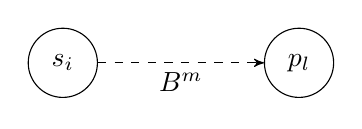
\begin{tikzpicture}[baseline=(si)]
\node[state] (si) {$s_i$};
\node[state,right of=si] (pl) {$p_l$};
\draw
(si) edge[dashed] node[below]{$B^m$} (pl)
;
\end{tikzpicture}
\end{itemize}

\subsection{Prepoznavanje završne konfiguracije}
\begin{propozicija}[{name=[treći fragment transpiliranog stroja]}]\label{pp:faza3}
Neka je $P$ RAM-program, i označimo $n:=n_P$, $m:=m_{P^1}$. Označimo s $f:=\kf{\kprog P}^1$ jednomjesnu funkciju koju $P$ računa. Tada postoji fragment Turingovog stroja takav da za sve $k\in\N$:
\begin{itemize}
    \item za sve $x\in\dom f$, prevodi reprezentaciju (\,$Turing_{kmn}$) početne konfiguracije s ulazom $x$ u reprezentaciju odgovarajuće završne konfiguracije;
    \item za sve $x\in{\dom f}\kompl$, počevši od reprezentacije početne konfiguracije s ulazom $x$, nikada ne stigne u stanje $s_n$.
\end{itemize}
\end{propozicija}
\begin{proof}
Za svaki $x\in\N$, označimo sa $(c_l)_l$ $P$-izračunavanje s $x$, i indukcijom po $l$ dokažimo da tako sastavljeni fragment Turingovog stroja dostigne konfiguraciju $Turing_{kmn}(c_l)$. Baza je primjena leme~\ref{lm:pi>si} (za $i=0$) na konfiguraciju koju smo dobili iz leme~\ref{lm:faza2}. Korak je primjena propozicije~\ref{prop:gadgets}. Dakle, ako $P$-izračunavanje stane u $l_0$ koraka, doći će u stanje $s_n$, u reprezentaciji završne konfiguracije $c_{l_0}$.

No vrijedi i obrat: u simulaciji jednog RAM-prijelaza $c\leadsto d$, naš fragment posjećuje samo stanja $p_i$, $s_i$ i $t_i$ za $i=c(\textsc{pc})$ ili za $i=d(\textsc{pc})$. Dakle, jedini način da dođe u stanje $s_n$ je da doista neka RAM-konfiguracija u izračunavanju preslika \textsc{pc} u $n$, a to znači da $P$-izračunavanje s $x$ stane.
\end{proof}

%Općenito, ovaj dio je na neki način najkompliciraniji (zbog broja stanja --- za tipični RAM-program ovaj fragment će biti višestruko veći od čitavog ostatka stroja $\mathcal T_0$; a i zbog činjenice da ne mora stati, odnosno doći u stanje $s_n$). S druge strane, možemo reći i da je najjednostavniji, jer ima vrlo uniformnu strukturu: fragmentići (u simulacijama obično se zovu \emph{gadgets}) za pojedine instrukcije su jednostavni i lijepo se slažu. Pogledajmo jednostavni primjer.

\begin{primjer}[{name=[treći fragment transpiliranog stroja]}]\label{pr:+a2}
U primjeru~\ref{pr:+a} smo vidjeli RAM-program $P_{\t a}$~\eqref{eq:+aprog} duljine $5$ i širine $2$, koji računa funkciju $\N\varphi_{\t a}(x):=2x+1$,  prateću funkciju dopisivanja \t a na kraj riječi.

$P_{\t a}$-izračunavanje s $\kr{\t{ab}}=4$ je ($c$ skraćeno zapisujemo kao $c(\reg0)c(\reg1)c(\textsc{pc})$)
\begin{multline}
    040\leadsto031\leadsto132\leadsto233\leadsto230\leadsto221\leadsto
    322\leadsto423\leadsto420\leadsto411\leadsto512\leadsto{}\\
    {}\leadsto613\leadsto
    610\leadsto601\leadsto702\leadsto803\leadsto800\leadsto804\leadsto
    905\lcirclearrowleft
%\begin{array}{r|cccccccccccccccccccc}
%i&0&1&2&3&4&5&6&7&8&9&10&11&12&13&14&15&16&17&18&\dotsm\\\hline
%c_i(\reg0)&
%0&0&1&2&2&2&3&4&4&4&5&6&6&6&7&8&8&8&9&9\\
%c_i(\reg1)&
%4&3&3&3&3&2&2&2&2&1&1&1&1&0&0&0&0&0&0&0\\
%c_i(\textsc{pc})&
%0&1&2&3&0&1&2&3&0&1&2&3&0&1&2&3&0&4&5&5
%\end{array}    
\end{multline}
s izlaznim podatkom $9=2\cdot4+1$, i odgovara mu (po preslikavanju $Turing_{225}$) šetnja kroz Turing-konfiguracije (ne pišemo, svima zajednički, početak \t{\renewcommand{\arraystretch}{0.1}\$\boo\boo\#})
\begin{multline}\label{eq:+a2}
\renewcommand{\arraystretch}{0.1}
\T{}{\mund{s_0}}{\boi}{\boi\boi\boi}\leadsto^*
\T{}{\mund{s_1}}{\boi}{\boi\boi}\leadsto^*
\T{}{\mund{s_2}}{\bii}{\boi\boi}\leadsto^*
\T{}{\mund{s_3}}{\bii}{\bii\boi}\leadsto^*
\T{}{\mund{s_0}}{\bii}{\bii\boi}\leadsto^*
\T{}{\mund{s_1}}{\bii}{\bii}\leadsto^*
\T{}{\mund{s_2}}{\bii}{\bii\bio}\leadsto^*
\T{}{\mund{s_3}}{\bii}{\bii\bio\bio}\leadsto^*
\T{}{\mund{s_0}}{\bii}{\bii\bio\bio}\leadsto^*
{}\\{}\leadsto^*
\renewcommand{\arraystretch}{0.1}
\T{}{\mund{s_1}}{\bii}{\bio\bio\bio}\leadsto^*
\T{}{\mund{s_2}}{\bii}{\bio\bio\bio\bio}\leadsto^*
\T{}{\mund{s_3}}{\bii}{\bio\bio\bio\bio\bio}\leadsto^*
\T{}{\mund{s_0}}{\bii}{\bio\bio\bio\bio\bio}\leadsto^*
\T{}{\mund{s_1}}{\bio}{\bio\bio\bio\bio\bio}\leadsto^*
\T{}{\mund{s_2}}{\bio}{\bio\bio\bio\bio\bio\bio}\leadsto^*
{}\\{}\leadsto^*
\renewcommand{\arraystretch}{0.1}
\T{}{\mund{s_3}}{\bio}{\bio\bio\bio\bio\bio\bio\bio}\leadsto^*
\T{}{\mund{s_0}}{\bio}{\bio\bio\bio\bio\bio\bio\bio}\leadsto^*
\T{}{\mund{s_4}}{\bio}{\bio\bio\bio\bio\bio\bio\bio}\leadsto^*
\T{}{\mund{s_5}}{\bio}{\bio\bio\bio\bio\bio\bio\bio\bio}
\,\text,
\end{multline}
koja se prirodno nastavlja na onu započetu u~\eqref{eq:+afaze} (kroz lemu~\ref{lm:pi>si} za $i=0$).

    Treći fragment Turingovog stroja koji odgovara $P_{\t a}$ prikazan je dijagramom
\begin{equation}
\begin{tikzpicture}[baseline=(s5)]
\node[state] (p0) {$p_0$};
\node[state,right of=p0] (s0) {$s_0$};
\node[state,right of=s0] (t0) {$t_0$};
\node[state,below=1.5 of p0] (p1) {$p_1$};
\node[state,below=1.5 of s0] (s1) {$s_1$};
%\node[state,below=1.5 of t0] (t1) {$t_1$};
\node[state,below=1.5 of p1] (p2) {$p_2$};
\node[state,below=1.5 of s1] (s2) {$s_2$};
%\node[state,below=1.5 of t1] (t2) {$t_2$};
\node[state,below=1.5 of p2] (p3) {$p_3$};
\node[state,below=1.5 of s2] (s3) {$s_3$};
%\node[state,below=1.5 of t2] (t3) {$t_3$};
\node[state,below=1.5 of p3] (p4) {$p_4$};
\node[state,below=1.5 of s3] (s4) {$s_4$};
%\node[state,below=1.5 of t3] (t4) {$t_4$};
\node[state,below=1.5 of p4] (p5) {$p_5$};
\node[state,below=1.5 of s4] (s5) {$s_5$};
%\node[state,below=1.5 of t4] (t5) {$t_5$};
\node[left=4 of p0,align=left] {$0.\;\decr14\;:$};
\node[left=4 of p1,align=left] {$1.\;\incr0\;:$};
\node[left=4 of p2,align=left] {$2.\;\incr0\;:$};
\node[left=4 of p3,align=left] {$3.\;\goto\;0\;:$};
\node[left=4 of p4,align=left] {$4.\;\incr0\;:$};
\draw
(p0) edge[loop left,dashed] node[left] {$B^2$} (p0)
(p0) edge node[below] {$\t\#$} (s0)
(p1) edge[loop left,dashed] node[left] {$B^2$} (p1)
(p1) edge node[below] {$\t\#$} (s1)
(p2) edge[loop left,dashed] node[left] {$B^2$} (p2)
(p2) edge node[below] {$\t\#$} (s2)
(p3) edge[loop left,dashed] node[left] {$B^2$} (p3)
(p3) edge node[below] {$\t\#$} (s3)
(p4) edge[loop left,dashed] node[left] {$B^2$} (p4)
(p4) edge node[below] {$\t\#$} (s4)
(p5) edge[loop left,dashed] node[left] {$B^2$} (p5)
(p5) edge node[below] {$\t\#$} (s5)
(s0) edge[loop above] node[below left,xshift=-4] {\t\textbullet\,\texttt@$1$} (s0)
(s0) edge[dashed] node[above] {\t\textopenbullet\,\texttt@$1$} (t0)
(t0) edge[dashed] node[above left,yshift=-4] {\t\textbullet:\t\textopenbullet\,\texttt@$1$} (p1)
(s1) edge[loop below] node[below] {\t\textbullet\,\texttt@$0$} (s1)
(s1) edge[dashed] node[above left,yshift=-3] {\t\textopenbullet:\t\textbullet\,\texttt@$0$} (p2)
(s2) edge[loop below] node[below] {\t\textbullet\,\texttt@$0$} (s2)
(s2) edge[dashed] node[above left,yshift=-3] {\t\textopenbullet:\t\textbullet\,\texttt@$0$} (p3)
(s4) edge[loop below] node[below] {\t\textbullet\,\texttt@$0$} (s4)
(s4) edge[dashed] node[above left,yshift=-3] {\t\textopenbullet:\t\textbullet\,\texttt@$0$} (p5)
(s3) edge[dashed,out=220,in=220,looseness=2] node[left] {$B^2$} (p0)
(t0) edge[out=267,in=20,looseness=1.5] node[right] {\t\#} (p4)
;
\end{tikzpicture}\text{\hspace{-2.7cm}%
.\,\qedhere%
}
\end{equation}
\end{primjer}

\begin{korolar}[{name=[prve tri faze transpiliranog stroja]}]\label{kor:faza3}
    Dosad izgrađeni Turingov stroj dostigne stanje $s_n$ ako i samo ako je pokrenut s ulazom $w\in\dom{\varphi_0}$, i u tom trenutku na traci nakon\, $\t\#$ u tragu $0$ piše $\t\textbullet^y\t\textopenbullet\dotsm$, gdje je $y=\N\varphi_0(\kr w)=\kr{\varphi_0(w)}$.
\end{korolar}
\begin{proof}
    Samo treba primijeniti propoziciju~\ref{pp:faza3} na RAM-program $P_0$ (dakle $f=\N\varphi_0$), na $x:=\kr w$ i $k:=\dulj{w}$. %Štoviše, jer se $f$ računa na $x$ koji jest kod, dovoljno je zahtijevati $f\approx\N\varphi_0$.
\end{proof}

\begin{napomena}[{name=[zaustavljanje transpiliranog stroja ovisi samo o trećoj fazi]}]\label{nap:snstane}
Ostatak Turingovog stroja koji konstruiramo vezat će se s dosad izgrađenim dijelom isključivo kroz stanje $s_n$, i njegovo računanje će uvijek stati, pa ćemo na kraju moći zaključiti da čitav Turingov stroj stane ako i samo ako dođe u stanje $s_n$, odnosno ako i samo ako je ulazna riječ u domeni od $\varphi_0$.
\end{napomena}

%Time smo riješili pitanje domene, i potrebno je još samo natrag dekodirati $y$ (ako postoji) u riječ $v:=\varphi_0(w)$, i postaviti je na početak trake.

\subsection{Dekodiranje izlazne vrijednosti}

Ovaj će postupak biti sličan onome u drugoj fazi, samo u obrnutom smjeru. Imamo broj $y$ zapisan unarno (pomaknuta baza $1$) u tragu $0$, i trebamo ga zapisati u pomaknutoj bazi $b'$ --- skidajući po jedan \t\textbullet\ iz traga $0$ i inkrementirajući riječ iz $\Sigma_0^*$ svaki put. Ipak, nekoliko tehničkih detalja čine ovaj postupak kompliciranijim.

Prvo, umjesto pisanja konstantnog znaka $r_1\in B^m$, morat ćemo čitati bilo koji znak koji u tragu $0$ ima \t\textbullet. Srećom, tehniku za to smo napravili (definicija~\ref{def:trag}).

Drugo i važnije, kod dekrementiranja smo znali da riječ neće postati dulja, te smo prazninama skraćivali broj koliko je već potrebno, dok ga nismo dekrementirali sasvim do nule. Kod inkrementiranja nemamo tu garanciju, i općenito se može dogoditi da puno puta moramo dodati po jednu znamenku slijeva (recimo, za $b'=5$, kad inkrementiramo $555$ u $1111$).

Zato je dobro riječ graditi unatrag, samo moramo biti sigurni da smo zauzeli dovoljno trake za to (da ne udarimo u lijevi rub, odnosno graničnik \t\$, prilikom dodavanja nove znamenke slijeva). Posljedica toga je da ne možemo učiniti intuitivno očitu stvar i upotrijebiti samo dio trake lijevo od separatora \t\#\ ---  jer je taj dio ograničen duljinom ulazne riječi, a izlazna riječ može biti puno dulja od ulazne.

Spasit ćemo se tako što ćemo za rekonstrukciju izlazne riječi upotrijebiti dio \emph{desno} od separatora, unutar kojeg smo simulirali $P_0$-izračunavanje s $w$. Taj dio će sigurno biti dovoljno dugačak, jer sadrži barem $y=\kr{\varphi_0(w)}$ znakova \t\textbullet\ u tragu $0$.

\begin{lema}[{name=[duljina riječi nije veća od koda riječi]}]\label{lm:dulj<=kr}
Za svaku riječ $u$ vrijedi $\dulj u\le\kr u$.
\end{lema}
\begin{proof}
Označimo s $b'$ broj znakova abecede $\Sigma$ nad kojom je riječ $w$.
Svaki pribrojnik u sumi~\eqref{eq:kodNSz} je pozitivan, jer je svaka znamenka $\N\Sigma(\alpha_i)\in[1\dd b']$, te je $b'>0$ zbog $\Sigma\ne\emptyset$. Dakle, svaki pribrojnik je barem $1$, pa je suma veća ili jednaka broju pribrojnika. No suma je po definiciji $\kr w$, a broj pribrojnika je upravo $n=\dulj w$.

Za $b'=1$ vrijedi jednakost (jer je jedina moguća znamenka $1$).
\end{proof}

Štoviše, lema~\ref{lm:dulj<=kr} pokazuje da riječ možemo dekodirati korak po korak: u svakom trenutku će nam u tragu $0$ ostati $y'$ znakova \t\textbullet, a od desnog kraja će biti napisana riječ $u'$ čiji je kod $\kr{u'}=y-y'$, pa će sigurno stati u prostor od $y-y'$ ćelija.

\begin{lema}[{name=[četvrti fragment transpiliranog stroja]}]\label{lm:faza4}
Postoji fragment Turingovog stroja koji prevodi reprezentaciju završne konfiguracije $(s_n,\dulj w+2,\t\$\bl^{\dulj w}\t\#t\bl\ldots)$, gdje $t$ u tragu $0$ ima oblik $\t\textbullet^y\t\textopenbullet^{z-y}$, u konfiguraciju $(q_3,\dulj w+1,\t\$\bl^{\dulj w}\t\#uv\t\$\bl\ldots)$, gdje je $\kr v=y$, te $u\in(B^m)^{z-\dulj{v}}$.
\end{lema}
\noindent\begin{gather*}
\SwapAboveDisplaySkip
\label{d:71}\tag{$\delta$4a}\delta(s_n,\gamma):=(s_n,\gamma,1)\text{, za sve } \gamma\in B^m_+:=B^m\setminus\{\bl\}\\
\label{d:72}\tag{$\delta$4b}\delta(s_n,\bl):=(q_3,\t\$,-1)\\
\label{d:73}\tag{$\delta$4c}\delta_{(0)}(q_3,\t\textopenbullet):=(q_3,\t\textopenbullet,-1)\\
\label{d:74}\tag{$\delta$4d}\delta_{(0)}(q_3,\t\textbullet):=(q_4,\t\textopenbullet,1)\\
\label{d:75}\tag{$\delta$4e}\delta(q_4,\alpha):=(q_4,\alpha,1)\text{, za sve }\alpha\in\Sigma_0\dcup B^m\\
\label{d:76}\tag{$\delta$4f}\delta(q_4,\t\$):=(q_5,\t\$,-1)\\
\label{d:77}\tag{$\delta$4g}\delta(q_5,\alpha_{b'}):=(q_5,\alpha_1,-1)\\
\label{d:78}\tag{$\delta$4h}\delta(q_5,\alpha_t):=(q_3,\alpha_{t+1},-1)\text{, za sve }t\in[1\dd b'\rangle\\
\label{d:79}\tag{$\delta$4i}\delta(q_5,\gamma):=(q_3,\alpha_1,-1)\text{, za sve }\gamma\in B^m\\
\label{d:70}\tag{$\delta$4j}\delta(q_3,\alpha):=(q_3,\alpha,-1)\text{, za sve }\alpha\in\Sigma_0
\end{gather*}

\begin{proof}
Kao što rekosmo, dokaz je sličan dokazu leme~\ref{lm:faza2}, samo u suprotnom smjeru. Prvo odemo do kraja upotrijebljenog (nepraznog) dijela trake~\eqref{d:71}, i tamo zapišemo krajnji graničnik~\eqref{d:72}. Zatim se krećemo ulijevo kroz znakove \t\textopenbullet\ u tragu $0$~\eqref{d:73} dok ne dođemo do \t\textbullet, koji maknemo~\eqref{d:74} i prenosimo ga desno kroz "znamenke" i "stupce bitova"~\eqref{d:75}, dok ne dođemo do krajnjeg graničnika~\eqref{d:76}. Tada se opet krećemo ulijevo, inkrementirajući riječ: zamjenjujući "devetke jedinicama"~\eqref{d:77}, te inkrementirajući prvu "ne-devetku"~\eqref{d:78}, ili ako takve nema, dodajući "jedinicu" slijeva~\eqref{d:79}. Zatim prođemo kroz ostale znamenke do "praznog prostora"~\eqref{d:70}, i opet izvršavamo cijeli postupak dok ne dođemo do separatora \t\#.
Argument zašto to funkcionira je praktički isti kao u dokazu leme~\ref{lm:faza2}. %Jedina bitna razlika je što je tamo~\eqref{dia:T2} "radni ciklus" imao dva stanja ($q_0$ i $q_1$), a ovdje ih ima tri ($q_3$, $q_4$ i $q_5$). To je posljedica toga da inkrementiramo "s krive strane", odnosno prenosimo kružiće slijeva nadesno, a kod kretanja zdesna nalijevo moramo pamtiti tražimo li tek znamenku koju ćemo inkrementirati (da bismo zamijenili "devetke jedinicama"), ili smo to već učinili (pa ostavljamo "devetke" na miru).
\end{proof}

\begin{primjer}[{name=[četvrti fragment transpiliranog stroja]}]
Za $\Sigma_0:=\{\t a,\t b,\t c,\t d\}$, četvrti fragment možemo prikazati dijagramom
\begin{equation}
\begin{tikzpicture}[baseline=(sn)]\label{dia:T4}
%\clip (-1,-2.53) rectangle (8.5,2.16);
\node[state] (sn) {$s_n$};
\node[state,right of=sn] (q5) {$q_3$};
\node[state,right of=q5] (q7) {$q_5$};
\node[state,above=1 of q7] (q6) {$q_4$};
\draw
(sn) edge[loop above] node[above] {$B^m_+$} (sn)
(sn) edge[dashed] node[above] {\bl:\t\$} (q5)
(q5) edge[loop above,dashed] node[above,xshift=-9,align=right] {\t\textopenbullet\,\texttt@$0$
\\[-1mm]
$\Sigma_0$} (q5)
(q5) edge node[above,xshift=-9,yshift=1] {\t\textbullet:\t\textopenbullet\,\texttt@$0$} (q6)
(q6) edge[loop right] node[right,align=left] {$B^m$
\\[-1mm]
$\Sigma_0$} (q6)
(q6) edge[dashed] node[right] {\t\$} (q7)
(q7) edge[dashed,loop right] node[right] {\t d:\t a} (q7)
(q7) edge[dashed] node[above,xshift=3] {\t a:\t b, \t b:\t c} node[below] {\t c:\t d, $B^m$:\t a} (q5)
;
\end{tikzpicture}\text{\;.\qedhere}
\end{equation}
\end{primjer}

Primijetimo da zbog $\kr v=y=\kr{\varphi_0(w)}$ i propozicije~\ref{pp:bijkr} zapravo vrijedi $v=\varphi_0(w)$, odnosno (ako uopće dođemo u situaciju da možemo primijeniti lemu~\ref{lm:faza4}) već imamo izlaznu riječ na traci. Još je treba premjestiti na početak, i obrisati s trake sve ostalo.

% \subsection{Pospremanje za sobom}

\begin{lema}[{name=[peti fragment transpiliranog stroja]}]\label{lm:faza5}
Postoji fragment Turingovog stroja koji prevodi konfiguraciju $(q_3,\dulj w+1,\t\$\bl^{\dulj w}\t\#uv\t\$\bl\ldots)$, gdje je $v\in\Sigma_0^*$, te $u\in(B^m)^*$, u konfiguraciju $(l_{\bl},\dulj v,v\bl\ldots)$.
\end{lema}
\noindent\begin{gather*}
    \SwapAboveDisplaySkip
\label{d:81}\tag{$\delta$5a}\delta(q_3,\t\#):=\delta(q_6,\gamma):=(q_6,\bl,1)\text{, za sve }\gamma\in B^m\\
\label{d:83}\tag{$\delta$5b}\delta(q_6,\alpha):=\delta(m_\alpha,\bl):=(m_\alpha,\bl,-1)\text{, za sve }\alpha\in\Sigma_0\\
    \label{d:85}\tag{$\delta$5c}\delta(m_\alpha,\beta):=(l_\alpha,\beta,1)\text{, za sve }\alpha\in\Sigma_0\dcup\{\bl\},\beta\in\Sigma_0\\
\label{d:86}\tag{$\delta$5d}\delta(m_\alpha,\t\$):=\delta(l_\alpha,\bl):=(q_6,\alpha,1)\text{, za sve }\alpha\in\Sigma_0\\
\label{d:87}\tag{$\delta$5e}\delta(q_6,\t\$):=\delta(m_{\bl},\bl):=(m_{\bl},\bl,-1)\\
%\label{d:88}\delta(m_{\bl},\alpha):=(l_{\bl},\alpha,1)\text{, za sve }\alpha\in\Sigma_0\\
\label{d:89}\tag{$\delta$5f}\delta(m_{\bl},\t\$):=(l_{\bl},\bl,-1)
\end{gather*}

\begin{proof}
Prvi korak je brisanje svih ostataka izračunavanja, i separatora, tako da na traci ostanu jedino izlazna riječ $v$ i dva graničnika --- početni i krajnji~\eqref{d:81}. Time dobivamo konfiguraciju $(q_6,l+1,\t\$\bl^l\,v\t\$\bl\ldots)$, gdje je $l:=\dulj w+\dulj u+1$.

Drugi korak je uzimanje jednog po jednog znaka od $v$, i njegov prijenos na početak trake~\eqref{d:83} --- s tim da će prvi znak od $v$ naići na početni graničnik i prebrisati ga~\eqref{d:86}, a svaki sljedeći znak će naići na onaj prije njega koji je već prenesen~\eqref{d:85}, i zapisati se desno od njega~\eqref{d:86}. Time dobijemo konfiguraciju $(q_6,l+\dulj v+1,v\bl^{l+1}\t\$\bl\ldots)$ ako je $v\ne\varepsilon$. Za $v=\varepsilon$, ovog koraka nema, odnosno odmah smo u konfiguraciji $(q_6,l+1,\t\$\bl^l\t\$\bl\ldots)$.

Treći korak počinje čitanjem i brisanjem završnog graničnika \t\$, i nastavlja prolaskom kroz praznine ulijevo~\eqref{d:87}, sve dok ne udarimo u zadnji znak od $v$ ako je $v\ne\varepsilon$~\eqref{d:85}, odnosno u početni graničnik (koji tada treba obrisati, ostavivši traku sasvim praznom) u slučaju $v=\varepsilon$~\eqref{d:89}.

U slučaju neprazne riječi $v$, očito će završna pozicija biti neposredno iza zadnjeg znaka od $v$, dakle $\dulj{v}$. U slučaju prazne riječi, prijelaz~\eqref{d:89} će se dogoditi na lijevom rubu trake, pokušati pomak lijevo, i ostati na istoj poziciji $0=\dulj{\varepsilon}=\dulj{v}$. U svakom slučaju dobili smo stanje $l_{\bl}$, traku $v\bl\ldots$\,, i poziciju $\dulj{v}$.
\end{proof}

\begin{primjer}[{name=[peti fragment transpiliranog stroja]}]
Za $\Sigma_0:=\{\t a,\t b\}$, peti fragment možemo prikazati dijagramom
\begin{equation}\label{dia:T5}
\begin{tikzpicture}[baseline=(q8)]
%\clip (-1,-2.53) rectangle (8.5,2.16);
\node[state] (q5) {$q_3$};
\node[state,below right of=q5] (q8) {$q_6$};
\node[state,left of=q8] (ma) {$m_{\t a}$};
\node[state,right of=q8] (mb) {$m_{\t b}$};
\node[state,below left of=q8] (la) {$l_{\t a}$};
\node[state,below right of=q8] (lb) {$l_{\t b}$};
\node[state,above right of=q8] (q9) {$m_{\bl}$};
\node[state,accepting,right of=q9] (qz) {$l_{\bl}$};
\draw
(q5) edge node[above,yshift=5] {\t\#:\bl} (q8)
(q8) edge[loop above] node[above,yshift=-3] {$B^m$:\bl} (q8)
(q8) edge[dashed,bend left] node[above] {\t a:\bl} (ma)
(ma) edge[bend left] node[below,yshift=2] {\t\$:\t a} (q8)
(q8) edge[dashed,bend right] node[above] {\t b:\bl} (mb)
(mb) edge[bend right] node[below,yshift=2] {\t\$:\t b} (q8)
(ma) edge[dashed,loop left] node[left] {\bl} (ma)
(mb) edge[dashed,loop right] node[right] {\bl} (mb)
(ma) edge node[left,xshift=2] {$\Sigma_0$} (la)
(mb) edge node[right] {$\Sigma_0$} (lb)
(la) edge node[below,xshift=3] {\bl:\t a} (q8)
(lb) edge node[below,xshift=-3] {\bl:\t b} (q8)
(q8) edge[dashed] node[right,xshift=1] {\t\$:\bl} (q9)
(q9) edge[dashed,loop left] node[left] {\bl} (q9)
(q9) edge[bend left] node[below] {$\Sigma_0$} (qz)
(q9) edge[bend right,dashed] node[above] {\t\$:\bl} (qz)
;
\end{tikzpicture}\text.
\end{equation}
Za općenitu abecedu $\Sigma_0$, umjesto dva "viseća trokuta" ispod $q_6$, bit će ih $b'$: po jedan $\triangle q_6 m_\alpha l_\alpha$ za svaki znak $\alpha\in\Sigma_0$.
\end{primjer}

%Primijetite da smo stigli do završnog stanja $l_{\bl}$. Time smo napokon završili konstrukciju Turingovog stroja $\mathcal T_0$, i sve je spremno za dokaz "obrata" teorema~\ref{tm:tikp}.

\subsection{Objedinjavanje}

\begin{teorem}[{name=[Turing-izračunljivost parcijalno rekurzivnih jezičnih funkcija]}]\label{tm:krit}
Neka je $\Sigma_0$ abeceda, $\N\Sigma_0$ njeno kodiranje, i $\varphi_0$ funkcija nad njom. Ako je $\N\varphi_0\in\mathscr Comp_1$, tada je $\varphi_0$ Turing-izračunljiva.
\end{teorem}
\begin{proof}
Po pretpostavci postoji RAM-program $P_0$ koji računa $\N\varphi_0$. Označimo $n:=n_{P_0}$ i $m:=m_{P_0^1}$. Tvrdimo da tada funkciju $\varphi_0$ računa Turingov stroj
\begin{align}
    &\qquad\mathcal T_0:=(Q,\Sigma_0,\Gamma,\bl,\delta,n_{\t\$},l_{\bl})\text,
\shortintertext{s komponentama}
    Q&:=\bdcup_{i\le6}\{q_i\}\dcup\bdcup_{i\le n}\{p_i,s_i,t_i\}\dcup\bdcup_{\mathclap{\alpha\in\Sigma_0\dcup\{\bl\}}}\,\{n_\alpha,m_\alpha,l_\alpha\}\dcup\{n_{\t\$},q_x\}\text,\\
    \Gamma&:=    \Sigma_0\dcup\{\t\$,\t\#\}\dcup B^m\text{, gdje je }B^m:=\prod_{i<m}\{\t\textopenbullet,\t\textbullet\}\text,\\
    \bl&:=(\t\textopenbullet,\t\textopenbullet,\dotsc,\t\textopenbullet)^\intercal\in B^m\text{ (zapisana kao stupac),}
\end{align}
    i funkcijom prijelaza $\delta$ zadanom jednakostima ($\delta\,\cdots$), %\eqref{d:11}--\eqref{d:12}, \eqref{d:21}--\eqref{d:28}, \eqref{d:31}--\eqref{d:61}, \eqref{d:71}--\eqref{d:70} i \eqref{d:81}--\eqref{d:89},
    tako da se svi parovi $(q,\alpha)\in(Q\setminus\{l_{\bl}\})\times\Gamma$ nenavedeni u tim jednakostima preslikavaju u $(q_x,\alpha,-1)$.

Doista, neka je $w\in\Sigma_0^*$ proizvoljna riječ, i označimo s $k:=\dulj{w}$ njenu duljinu. Promotrimo prvo slučaj kada je $w\in\dom{\varphi_0}$.

    Tada će početnu konfiguraciju $(n_{\t\$},0,w\bl\ldots)$ prvi fragment od $\mathcal T_0$ (lema~\ref{lm:faza1}) prebaciti u $(q_0,k,\t\$w\t\#\bl\ldots)$, a nju će pak drugi fragment prebaciti u $(p_0,k+2,\t\$\bl^k\,\t\#r_1^{\kr w}\bl\ldots)$, gdje je $r_1=(\t\textopenbullet,\t\textbullet,\t\textopenbullet,\dotsc,\t\textopenbullet)^\intercal$ (lema~\ref{lm:faza2}). Kako je $w\in\dom{\varphi_0}$, vrijedi $x:=\kr w\in\dom{\N\varphi_0}$, pa $P_0$-izračunavanje s $x$ stane, i izlazni podatak mu je $y:=\N\varphi_0(x)=\kr{\varphi_0(w)}$. Prema korolaru~\ref{kor:faza3}, $\mathcal T_0$-izračunavanje s $w$ (treća faza) će zato doći u konfiguraciju $(s_n,k+2,\t\$\bl^k\,\t\#t\bl\ldots)$, gdje $t$ u tragu $0$ ima oblik $\t\textbullet^y\t\textopenbullet^{z-y}$. Tu će pak konfiguraciju četvrti fragment (lema~\ref{lm:faza4}) prebaciti u $(q_3,k+1,\t\$\bl^k\,\t\#uv\t\$\bl\ldots)$, gdje je $v=\varphi_0(w)$, te $u\in(B^m)^{z-\dulj{v}}$. Peti će fragment (lema~\ref{lm:faza5}) napokon prebaciti tu konfiguraciju u završnu konfiguraciju $(l_{\bl},\dulj{v},v\bl\ldots)$, gdje se na traci nalazi izlazni podatak $\varphi_0(w)$.

    Ako pak $w\notin\dom{\varphi_0}$, tada će se prve dvije faze izvršiti jednako, ali iz $x\notin\dom{\N\varphi_0}$ slijedi da $P_0$-izračunavanje s $x$ nikad neće stati, pa po korolaru~\ref{kor:faza3} niti $\mathcal T_0$-izračunavanje neće doći do $s_n$. Prema napomeni~\ref{nap:snstane}, to znači da ono nikad neće stati (doći do $l_{\bl}$), jer jedini put od $n_{\t\$}$ do $l_{\bl}$ vodi kroz stanje $s_n$.
\end{proof}

Primijetimo iznenađujuću sličnost upravo provedenog dokaza s dokazom propozicije~\ref{prop:semfmacro} (semantika funkcijskog makroa). Kao što smo tamo omogućili makro-stroju da u izoliranoj okolini izvrši neki konkretni RAM-program, tako smo to ovdje omogućili Turingovom stroju. Kao i u makro-programu iz definicije~\ref{def:funmakro}, postupak se sastoji od pet faza: "otvaranje okvira" pomicanjem udesno, prijenos (kodiranje) argumenata u simulaciju (namještanje početne konfiguracije), sama simulacija (izvršavanje pojedinih instrukcija RAM-programa), te ako ona stane, prijenos (dekodiranje) njene povratne vrijednosti iz završne konfiguracije, i "zatvaranje okvira" (pospremanje nereda koji smo napravili).

Prikažimo postupak Turing-iz\-ra\-ču\-na\-va\-nja kroz faze (sa $z$ je označen najveći broj u ikojem relevantnom registru od $\mathcal S_0$ u završnoj konfiguraciji $P_0$-izračunavanja s $\kr w$):
\begin{equation}
\begin{array}{l|ccl}
                             &\text{stanje}&\text{pozicija}&\text{traka}\\\hline
    \text{početna konfiguracija} & n_{\t\$} & 0         & w\bl\ldots \\
\text{nakon prve faze}       & q_0 & \dulj w   & \t\$w\t\#\bl\ldots \\
\text{nakon druge faze}      & p_0 & \dulj w+2 & \t\$\bl^{\dulj w}\t\#r_1^{\kr w}\bl\ldots \\
\text{nakon treće faze}      & s_n & \dulj w+2 & \renewcommand{\arraystretch}{0.1}
    \t\$\bl^{\dulj w}\t\#\begin{array}{@{}c@{}}\t\textbullet\\?\end{array}^{\kr{v}}?^{z-\kr{v}}\bl\ldots\\
\text{nakon četvrte faze}    & q_3 & \dulj w+1 &
\renewcommand{\arraystretch}{0.1}
\t\$\bl^{\dulj w}\t\#\begin{array}{@{}c@{}}\t\textopenbullet\\?\end{array}^{z-\dulj v}v\t\$\bl\ldots\\
\text{prvi korak pete faze} & q_6 & \dulj w+2+z-\dulj v       & \t\$\bl^{\dulj w+1+z-\dulj v}v\t\$\bl\ldots\\
\text{drugi korak pete faze}& q_6 & \dulj w+2+z & v\bl^{\dulj w+2+z-\dulj v}\t\$\bl\ldots\\
\text{završna konfiguracija} & l_{\bl} & \dulj v   & v\bl\ldots
\end{array}
\end{equation}

\begin{primjer}[{name=[transpilirani stroj dodaje znak na kraj riječi]}]\label{pr:+a3}
Primjer~\ref{pr:+a} sad možemo pratiti kroz sve faze:
\begin{align}
    \text{ulaz}&&&\T{}{n_{\t\$}}{a}{b}\\
\text{uokvirivanje ulaza}&&{}\leadsto^*{}&\T{\$a}{q_0}{b}{\#}\\
\kr{\t{ab}}=(12)_2=4&&\leadsto^*{}&
\renewcommand{\arraystretch}{0.1}
\T{\$\bl\bl\#}{\mund{p_0}}{\boi}{\boi\boi\boi}\\
    2\cdot4+1=9\text{; raspisano u~\eqref{eq:+a2}}&&{}\leadsto^*{}&
\renewcommand{\arraystretch}{0.1}
 \T{\$\bl\bl\#}{\mund{s_5}}{\bio}{\bio\bio\bio\bio\bio\bio\bio\bio}\\
9=(121)_2=\kr{\t{aba}}&&{}\leadsto^*{}&
\renewcommand{\arraystretch}{0.1}
 \T{\$\bl\bl}{q_3}{\#}{\bl\bl\bl\bl\bl\bl aba}\\
\text{uokvirivanje izlaza}&&{}\leadsto^*{}&
\renewcommand{\arraystretch}{0.1}
\T{\$\bl\bl\bl\bl\bl\bl\bl\bl\bl}{q_6}{a}{ba\$}\\
\text{premještanje izlaza}&&{}\leadsto^*{}&
\renewcommand{\arraystretch}{0.1}
\T{aba\bl\bl\bl\bl\bl\bl\bl\bl\bl\bl}{q_6}{\$}{}\\
\text{izlaz}&&{}\leadsto^*{}&
\T{aba}{l_{\bl}}{\bl}{}\lcirclearrowleft\text.
\end{align}

Naravno, dodati \t a na kraj riječi Turingov stroj može puno jednostavnije --- ali ovaj primjer zapravo pokazuje kako može računati bilo koju funkciju koju RAM-stroj može računati. Pravo računanje odvija se u primjeru~\ref{pr:+a2} --- ovo je samo hrpa "papirologije" prije i poslije, koju treba riješiti da bi taj primjer bio koristan.
\end{primjer}

Ukratko, dokazali smo da je za \emph{jezične} funkcije izračunljivost u jezičnom modelu jednako snažna kao izračunljivost njihovih pratećih funkcija u brojevnom modelu. Primijetimo da smo time napokon opravdali neovisnost o korištenom \emph{encodingu}, i riješili "filozofski problem" s početka točke~\ref{sec:kSigma}.

\begin{korolar}[{name=[neovisnost izračunljivosti jezične funkcije o kodiranju abecede]}]\label{kor:ikojiNSigma}
Neka je $\Sigma$ abeceda, te $\varphi$ jezična funkcija nad njom.\newline Tada parcijalna rekurzivnost funkcije $\N\varphi$ ne ovisi o izboru kodiranja $\N\Sigma$.
\end{korolar}
\begin{proof}
Neka su $\N\Sigma$ i $\N'\Sigma$ dva kodiranja $\Sigma$. Ako je $\N\varphi_0$ parcijalno rekurzivna, tada je po teoremu~\ref{tm:pir} RAM-izračunljiva. Tada je po teoremu~\ref{tm:krit} (primijenjenom na kodiranje $\N\Sigma$) $\varphi$ Turing-izračunljiva, a onda je po teoremu~\ref{tm:tikp} (primijenjenom na kodiranje $\N'\Sigma$) $\N'\varphi$ parcijalno rekurzivna. Potpuno isto (zamjenom ta dva kodiranja) se dokaže drugi smjer, dakle $\N\varphi$ je parcijalno rekurzivna ako i samo ako je $\N'\varphi$ parcijalno rekurzivna.
\end{proof}

%\section{Turing-izračunljivost brojevnih funkcija}
\section{Izračunljivost jezikâ}\label{sec:Todl}

% Ivanov prijedlog: koristiti zareze umjesto / za separator.
% Nisam siguran kako to sklopiti s nulama u nizu ali možda nije strašno.

Sve dosad napravljeno može se iskazati u jednom vrlo općenitom obliku.

\begin{propozicija}[{name=[izomorfizam skupova $\TComp$ i $\mathscr Comp_1$]}]\label{pp:trackbij}
Neka je $\Sigma$ proizvoljna abeceda te $\N\Sigma$ proizvoljno njeno kodiranje. Tada je $\varphi\mapsto\N\varphi$ bijekcija između skupa $\TComp$ svih Turing-izračunljivih jezičnih funkcija nad $\Sigma$, i skupa $\mathscr Comp_1$ svih jednomjesnih RAM-izračunljivih funkcija.
\end{propozicija}

\begin{proof}
Teorem~\ref{tm:tikp} (zajedno s teoremom~\ref{tm:pir}) kaže da za svaku $\varphi\in\TComp$ vrijedi $\N\varphi\in\mathscr Comp_1$. Dakle preslikavanje doista "ide kamo treba".

Za injektivnost, neka su $\varphi_1,\varphi_2\in\TComp$ različite. Ako imaju različite domene, bez smanjenja općenitosti možemo pretpostaviti da postoji $w\in\dom{\varphi_1}\!\!\setminus\dom{\varphi_2}$. Tada je $\kr w\in\dom{\N\varphi_1}$, ali isto tako $\kr w\notin\dom{\N\varphi_2}$ jer je kodiranje riječi injekcija, pa $\kr w$ ne može biti jednak nijednom $\kr{w'}$ za $w'\in\dom{\varphi_2}$. To znači da prateće funkcije $\N\varphi_1$ i $\N\varphi_2$ imaju različite domene, pa su različite.

Ako pak $\varphi_1$ i $\varphi_2$ imaju istu domenu, ali se razlikuju na nekoj riječi $w$ iz te domene, tada (opet po injektivnosti kodiranja riječi) vrijedi
\begin{equation}
    \N\varphi_1(\kr w)=\kr{\varphi_1(w)}\ne\kr{\varphi_2(w)}=\N\varphi_2(\kr w)\text,
\end{equation}
pa su $\N\varphi_1$ i $\N\varphi_2$ različite jer se razlikuju na elementu $\kr w$.

Za surjektivnost, uzmimo proizvoljnu $\f F^1\in\mathscr Comp_1$ i tražimo $\varphi\in\TComp$ takvu da je $\f F=\N\varphi$. Očito, u domeni joj moraju biti upravo sve riječi $w$ za koje je $\kr w\in\dom{\f F}$, a svaku takvu riječ mora preslikavati u (jedinstvenu) riječ $v$ čiji kod je $\f F(\kr w)$. Time je jezična funkcija $\varphi$ potpuno određena, a iz $\N\varphi=\f F\in\mathscr Comp_1$ po teoremu~\ref{tm:krit} slijedi $\varphi\in\TComp$. Dobivenu funkciju $\varphi$ označavamo s $\N^{-1}\f F$.
\end{proof}
Precizno, za $\sigma:=\N\Sigma^*$, imamo vezu
%\begin{equation}
	$\f F=\N\varphi=\sigma\circ\varphi\circ\sigma^{\,-1}\Longleftrightarrow
	\varphi=\N^{-1}\f F=\sigma^{\,-1}\circ\f F\circ\sigma$
%\end{equation}
te vrijedi $\N\,\N^{-1}\f F=\f F$ i $\N^{-1}\N\varphi=\varphi$.

\begin{korolar}[{name=[jednomjesne brojevne funkcije u različitim modelima]}]\label{kor:pent}
Neka je $\Sigma$ abeceda s kodiranjem $\N\Sigma$ te $F^1$ brojevna funkcija.

Tada je $F$ parcijalno rekurzivna ako i samo ako je $\N^{-1}F$ Turing-izračunljiva.
\end{korolar}
\begin{proof}
Ako je $F=\N\,\N^{-1}F$ parcijalno rekurzivna, tada je po teoremu~\ref{tm:pir} RAM-izračunljiva, pa je po teoremu~\ref{tm:krit} $\N^{-1}F$ Turing-izračunljiva. S druge strane, ako je $\N^{-1}F$ Turing-izračunljiva, onda je po teoremu~\ref{tm:tikp} $\N\,\N^{-1}F=F$ parcijalno rekurzivna.
\end{proof}

Vidimo da korolar~\ref{kor:pent} vrijedi bez obzira na abecedu i kodiranje. Važan posebni slučaj dobijemo za jednočlanu abecedu, za koju je kodiranje jedinstveno i podudara se s duljinom (lema~\ref{lm:dulj<=kr}).

\begin{definicija}[{name=[unarna abeceda i unarna reprezentacija brojevne funkcije]}]
\emph{Unarna abeceda} je $\Sigma_{\t\textbullet}:=\{\t\textbullet\}$, s kodiranjem %. Kad nema opasnosti od zabune, umjesto $\Sigma_{\t\textbullet}$ pišemo samo \t\textbullet. Kodiranje unarne abecede je jedino moguće: 
	$\N\Sigma_{\t\textbullet}(\t\textbullet):=1$.

	Za jednomjesnu brojevnu funkciju $F^1$, jezičnu funkciju $\N^{-1}F$ nad $\Sigma_{\t\textbullet}$ zovemo \emph{unarnom reprezentacijom} od $F$ i označavamo je $\t\textbullet F$.
\end{definicija}

Svaka riječ $u$ nad unarnom abecedom ($u\in\Sigma_{\t\textbullet}^*$) je oblika $u=\t\textbullet^n$, gdje je $n=\dulj u=\kr u$. Sada definicija preslikavanja $\N^{-1}$ kaže da je $\t\textbullet F(\t\textbullet^n)=\t\textbullet^{F(n)}$ ako je $n\in\dom F$, a $\t\textbullet^n\notin\dom{\t\textbullet F}$ inače. Po napomeni~\ref{nap:parcdef}, pišemo
$\t\textbullet F(\t\textbullet^n)\simeq\t\textbullet^{F(n)}$.

\begin{primjer}[{name=[unarna reprezentacija]}]
$\t\textbullet\f{factorial}\bigl(
\t\textbullet\f{prime}(
\t\textbullet)
\bigr)=\t\textbullet\f{factorial}(
\t{\textbullet\textbullet\textbullet})
=\t{\textbullet\textbullet\textbullet\textbullet\textbullet\textbullet}$, jer je $p_1!=3\,!=6$.\newline
	Za inicijalne funkcije, $\t\textbullet\f I_1^1(w)=w$, $\t\textbullet\f{Sc}(w)=w\t\textbullet$, a $\t\textbullet\f Z(w)=\varepsilon$ za sve $w\in\Sigma_{\t\textbullet}^*$. %Za parcijalne funkcije, $\varepsilon\notin\dom{\t\textbullet\f{Russell}}$, jer $0\notin K$.
\end{primjer}

\begin{korolar}[{name=[unarno reprezentirane brojevne funkcije u različitim modelima]}]\label{kor:peuf}
Neka je $F^1$ brojevna funkcija.
	
	Tada je $F$ parcijalno rekurzivna ako i samo ako je $\t\textbullet F$ Turing-izračunljiva.
\end{korolar}
\begin{proof}
Već rekosmo, ovo je posebni slučaj korolara~\ref{kor:pent}, za unarnu abecedu.
\end{proof}

%\subsection{Izračunljivost jezika}\label{sec:Todl}

Neka je $\Sigma$ proizvoljna abeceda, s $b'$ znakova, $\N\Sigma$ njeno kodiranje te $L\subseteq\Sigma^*$ jezik nad njom. Što bi značilo da je $L$ izračunljiv?

Izračunljivost $L$ u brojevnom modelu gledamo preko kodova: definiramo jednomjesnu brojevnu relaciju
\begin{equation}\label{eq:kodLdef}
    \kr L:=\{\kr w\mid w\in L\}=\N\Sigma^*[L]\text,
\end{equation}
i prirodno je reći da $L$ ima neko svojstvo izračunljivosti (npr.\ da je primitivno rekurzivan) ako relacija $\kr L$, odnosno njena karakteristična funkcija $\chi_{\kr L}$, ima to svojstvo.

Recimo, prazan jezik $\emptyset$ je primitivno rekurzivan jer je $\chi_{\kr\emptyset}\!=\chi_{\mspace{1mu}\emptyset}\!=\!\f Z$ primitivno rekurzivna (čak inicijalna). Također, univerzalni jezik $\Sigma^*$ je primitivno rekurzivan, jer je $\kr{\Sigma^*}=\N\Sigma^*[\Sigma^*]=\im{\N\Sigma^*}\!=\N$, čija je karakteristična funkcija $\f C_1^1=\f{Sc}\circ\f Z$.

U jezičnom modelu, moramo vidjeti što znači da neki Turingov stroj računa $\chi_L$. To je Turingov stroj nad $\Sigma$, i ulaz $w\in\Sigma^*$ mu se daje na isti način kao i običnom Turingovom stroju: kroz početnu konfiguraciju $(q_0,0,w\bl\ldots)$. No za izlaz ($\mathit{true}$ ili $\mathit{false}$, ovisno o tome je li $w\in L$) postoji samo konačno mnogo mogućnosti, pa ga je prirodnije predstaviti stanjem. Zato takvi Turingovi strojevi imaju \emph{dva} završna stanja, $q_a$ i $q_r$, kojima signaliziraju je li riječ u jeziku ili nije (kažemo da \emph{prihvaćaju} odnosno \emph{odbijaju} riječ).

Na prvi pogled, to je slično stanjima $q_z$ i $q_x$ koje smo imali u našim Turingovim strojevima, samo što konfiguracija sa stanjem $q_r$ (kao i ona s $q_a$) prelazi u samu sebe, a ne po funkciji~$\delta$. Ali postoji jedna bitna razlika: kako su karakteristične funkcije nužno totalne, od takvih strojeva zahtijevamo da \textbf{uvijek stanu} (za svaki ulaz dostignu konfiguraciju s jednim od ta dva završna stanja) i zovemo ih \emph{odlučiteljima} (\emph{deciders}). Svaki odlučitelj $\mathcal T$ dijeli $\Sigma^*$ na dva dijela,
\begin{align}
    \SwapAboveDisplaySkip
    L(\mathcal T):=\{w\in\Sigma^*&\mid\text{$\mathcal T$\!-izračunavanje s $w$ stane u stanju $q_a$}\}
    \text{ i}\\ \bigl(L(\mathcal T)\big)\kompl=\{w\in\Sigma^*&\mid\text{$\mathcal T$\!-izračunavanje s $w$ stane u stanju $q_r$}\}\text,
\end{align} i kažemo da \emph{prepoznaje} $L(\mathcal T)$.

Nije preteško vidjeti da su te dvije karakterizacije, brojevna i jezična, povezane --- pogotovo jer već imamo napravljen najveći dio posla.

\begin{teorem}[{name=[rekurzivnost Turing-odlučivog jezika]}]\label{tm:oikr}
    Neka je $L$ jezik (nad nekom abecedom $\Sigma$).\newline Ako postoji Turingov odlučitelj koji prepoznaje $L$, tada je relacija $\kr L$ rekurzivna.
\end{teorem}
\begin{proof}
Pretpostavimo da je $\mathcal T$ odlučitelj za $L$ i provedimo s tim strojem postupak iz točke~\ref{sec:tikp}. Ovdje navodimo samo detalje koje je potrebno promijeniti.

Prvo, kako imamo dva završna stanja, moramo fiksirati njihove kodove: recimo, $\N Q(q_a):=1$, a $\N Q(q_r):=2$. (Dokažite analogon leme~\ref{lm:bsomp-q0neqz}, da bez smanjenja općenitosti možemo pretpostaviti $q_0\ne q_a$ i $q_0\ne q_r$ --- a po definiciji odlučitelja mora biti $q_a\ne q_r$.)

    Drugo, kako nam $\delta$ sad nije definirana na oba završna stanja, treba promijeniti uvjet u lemi analognoj lemi~\ref{lm:newssdprn}, u $q\notin\{q_a,q_r\}$. Tu se ništa bitno ne mijenja, osim što će $\f{direction}$-tablica (vidjeti primjer~\ref{pr:polatable}) imati dva retka jedinicâ, a ne samo jedan.

I treće, umjesto parcijalno rekurzivne funkcije $\f{stop}$ imat ćemo funkciju zadanu sa
\begin{equation}\label{eq:stop'def}
    \f{stop}'(x):=\mu n\bigl(\f{State}(x,n)\in\{1,2\}\bigr)\text,
\end{equation}
	za koju ćemo moći zaključiti da je rekurzivna. Naime, parcijalno je rekurzivna kao minimizacija rekurzivne (lema~\ref{lm:StateHeadTapeprn} i korolar~\ref{kor:konprn}) relacije. Totalna je (pa smo u~\eqref{eq:stop'def} mogli koristiti \enquote*{:=}) po definiciji odlučitelja: ako je $x=\kr w$, tada mora za neki $n$ biti $\f{State}(x,n)\in\{1,2\}$, jer $\mathcal T$\!-izračunavanje s $w$ mora stati --- i $\f{stop}'(x)=\f{stop}'(\kr w)$ je upravo broj koraka nakon kojeg ono stane.

Tvrdimo da je
\begin{equation}
	x\in\kr L\Longleftrightarrow\f{State}\mspace{2mu}\bigl(x,\f{stop}'(x)\bigr)=1\text,
\end{equation}
iz čega slijedi rekurzivnost od $\kr L$ po lemi~\ref{lm:comprek} i korolaru~\ref{kor:prnrek}.

Doista, ako je $x\in\kr L=\N\Sigma^*[L]$, to znači da postoji $w\in L$ takva da je $x=\kr w$. Tada $\mathcal T$\!-izračunavanje s $w$ mora stati u stanju $q_a$ --- označimo s $n_0$ broj koraka nakon kojeg se to dogodi. Tada je $\f{State}(x,n_0)=1\in\{1,2\}$, dok za sve $n<n_0$ konfiguracija nakon $n$ koraka nije završna (sasvim analogno propoziciji~\ref{prop:ram1zav} --- jer završne konfiguracije prelaze isključivo u same sebe, postoji najviše jedna završna konfiguracija u izračunavanju) pa $\f{State}(x,n)\notin\{1,2\}$. Dakle $n_0=\f{stop}'(x)$, pa je $\f{State}\bigl(x,\f{stop}'(x)\bigr)=\f{State}(x,n_0)=1$.

U drugom smjeru, pretpostavimo $\f{State}\bigl(x,\f{stop}'(x)\bigr)=1$. Po propoziciji~\ref{pp:bijkr}, postoji jedinstvena riječ $w\in\Sigma^*$ takva da je $x=\kr w$. $\mathcal T$ je odlučitelj, pa $\mathcal T$\!-izračunavanje s $w$ mora stati --- označimo s $n_0$ broj koraka nakon kojeg se to dogodi. Tada je (kao i prije) $\f{State}(x,n)\notin\{1,2\}$ za $n<n_0$, a $\f{State}(x,n_0)=1\in\{1,2\}$, pa je $\f{stop}'(x)=n_0$. Sada pretpostavka glasi $\f{State}(x,n_0)=1$, odnosno završno stanje je $q_a$, pa $\mathcal T$ prihvaća $w$. To znači da je $w\in L$, odnosno $x=\kr w\in\kr L$.
\end{proof}
%\newpage

\begin{teorem}[{name=[Turing-odlučivost rekurzivnog jezika]}]\label{tm:krio}
Neka je $L$ jezik (nad nekom abecedom $\Sigma$).\newline Ako je relacija $\kr L$ rekurzivna, tada postoji Turingov odlučitelj za $L$.
\end{teorem}
\begin{proof}
Pretpostavka zapravo znači da je $\chi_{\kr L}$ rekurzivna funkcija. Dakle $\chi_{\kr L}$ je parcijalno rekurzivna, pa po teoremu~\ref{tm:pir} postoji RAM-program $P$ koji je računa; i totalna je, pa $P$-izračunavanje stane sa svakim ulazom. Na $P$ bismo htjeli primijeniti postupak iz točke~\ref{sec:RAM>Turing} --- dakle moramo $\chi_{\kr L}$ prikazati kao $\N\varphi$ za neku jezičnu funkciju $\varphi$ nad $\Sigma$. Možemo li to?

Svakako: dokaz propozicije~\ref{pp:trackbij} kaže da je $\varphi:=\N^{-1}\chi_{\kr L}=\sigma^{\,-\!1}\circ\chi_{\kr L}\circ\sigma$, uz oznaku $\sigma:=\N\Sigma^*$. Funkcija $\varphi$ je totalna kao kompozicija tri totalne, a Turing-izračunljiva je prema korolaru~\ref{kor:pent} (ako uzmemo isto kodiranje pomoću kojeg smo izračunali $\kr L$). Pogledajmo detaljnije kako ona djeluje.

Ako joj damo riječ $w\in\Sigma^*\setminus L$, tada ($\mspace{-1mu}\sigma$ je injekcija) vrijedi $\kr w\notin\kr L$, pa je $\chi_{\kr L}(\kr w)=0$. Tada je
\begin{equation}
    \varphi(w)=\sigma^{\,-\!1}\bigl(\,\chi_{\kr L}\bigl(\sigma(w)\bigr)\bigr)=\sigma^{\,-\!1}\bigl(\,\chi_{\kr L}(\kr w)\bigr)=\sigma^{\,-\!1}(0)=\varepsilon\text.
\end{equation}
Dakle, riječi izvan $L$ ona preslikava u praznu riječ. Riječi \emph{unutar} $L$ onda ne smije preslikavati u $\varepsilon$ zbog injektivnosti $\sigma^{\,-\!1}$, a jer je totalna, mora ih preslikavati nekamo. Dakle, $\varphi(w)$ je neprazna riječ za svaku $w\in L$. Vidimo da, baš kao i u $\N$, imamo prirodnu reprezentaciju $bool$ u $\Sigma^*$: prazna riječ je lažna, neprazne su istinite. Mnogi programski jezici koji definiraju istinitost stringova, definiraju je upravo na taj način.

%Kako izvršavanje RAM-programa o kojem govorimo stane za svaki $\kr w$, po korolaru~\ref{kor:faza3} i napomeni~\ref{nap:snstane} slijedi da će Turingov stroj koji konstruiramo stati za svaki $w$ --- samo trebamo malo promijeniti način na koji stane, da ne komunicira izlaz putem trake nego putem završnog stanja.

    Naš Turingov stroj koji računa $\varphi$ dobiven je transpiliranjem RAM-programa $P$ koji računa $\chi_{\kr L}$. Srećom, u završnoj konfiguraciji pozicija mu je $0$, pa je vrlo lako vidjeti je li izlazna riječ prazna: znak koji čitamo tada je ili praznina ili element ulazne abecede. Proglasimo $l_{\t\$}$ običnim stanjem, i dodajmo prijelaze %U opisu pete (posljednje) faze rada tog Turingovog stroja, razlikovali smo slučajeve kad je izlazna riječ prazna i kad nije. Kao što smo upravo vidjeli, to nam može poslužiti za odabir završnog stanja u kojem ćemo završiti --- samo zamijenimo prijelaze iz $m_{\t\$}$ s
\begin{gather}
    %\SwapAboveDisplaySkip
\label{eq:d88j}\tag{$\delta$5b}
    \delta(l_{\t\$},\alpha):=(q_a,\bl,-1)\text{, za sve }\alpha\in\Sigma\text,\\
\label{eq:d89j}\tag{$\delta$5c}
    \delta(l_{\t\$},\bl):=(q_r,\bl,-1)\text.
\end{gather}
Po teoremu~\ref{tm:krit}, dobiveni stroj će "računati" (pod navodnicima jer odlučitelji zapravo ne služe za računanje funkcija) funkciju $\varphi$, pa će za $w\in L$ rezultat biti neprazan. To znači da će stroj na kraju izračunavanja čitati znak iz $\Sigma$ i ući u stanje $q_a$. Za $w\notin L$ rezultat će biti $\varepsilon$ pa će stroj pročitati prazninu i ući u stanje $q_r$. Budući da za svaku riječ $w\in\Sigma^*$ vrijedi jedna od te dvije mogućnosti, zaključujemo da smo doista konstruirali odlučitelj.
\end{proof}
\vspace{-3mm}

Dijagramatski, na kraj Turingovog stroja dodali smo fragment\; %gornji desni kut~\eqref{dia:T5} zamijenimo s\quad
\begin{tikzpicture}[baseline=(q9.base)]\label{dia:T5j}
    \node[state] (q9) {$l_{\t\$}$};
\node[state,accepting,right of=q9] (qt) {$q_a$};
\node[state,accepting,below right=0.5 and 1.6 of q9] (qf) {$q_r$};
\draw
%(q9) edge[dashed,loop left] node[left] {\t/:\bl} (q9)
(q9) edge[dashed] node[above] {$\Sigma$:\bl} (qt)
(q9) edge[dashed] node[below] {\bl} (qf)
;
\end{tikzpicture}\;.
\vspace{-8mm}

\section{Turing-izračunljivost višemjesnih funkcija}

Dosadašnji rezultati pokazuju da je za jezične funkcije, i za \emph{jednomjesne} brojevne funkcije, svejedno računamo li ih na Turingovom stroju ili na nekom brojevnom modelu izračunavanja (npr.\ RAM-stroju). Da bismo isto dokazali i za \emph{višemjesne} brojevne funkcije, trebamo precizirati reprezentaciju njihovih ulaza.

%Zapravo, sve potrebne ideje smo već vidjeli. Za ulazne podatke jednomjesnih funkcija, kao i za izlazne podatke, koristit ćemo unarni zapis: što je prirodnije nego broj $4$ zapisati na traku Turingovog stroja kao \textbullet\textbullet\textbullet\textbullet, a $0$ kao praznu riječ $\varepsilon$\@? Tako smo već prikazivali (u tragovima) sadržaj registara kod simulacije RAM-izračunavanja. Da smo opterećeni složenošću, morali bismo koristiti binarni ili neki drugi "pravi" pozicijski zapis, ali srećom nismo.

Već smo u uvodu nagovijestili, koristit ćemo kontrakciju --- u abecedu ćemo dodati separator \t/ kojim ćemo razdvojiti više ulaznih podataka: npr.\ $(1,0,5,0)$ prenijet ćemo kao \t{\textbullet//\textbullet\textbullet\textbullet\textbullet\textbullet/}.

\begin{definicija}[{name=[binarna abeceda i binarna reprezentacija]}]\label{def:beta}
\emph{Binarna abeceda} je abeceda $\Sigma_\beta:=\{\t\textbullet,\t/\}$. Za svaki neprazni konačni niz prirodnih brojeva $\vec x=(x_1,x_2,\dotsc,x_k)$, definiramo \emph{binarnu reprezentaciju} kao
\begin{equation}\label{eq:betadef}
    \beta(\vec x):=\t\textbullet^{x_1}\t/\t\textbullet^{x_2}\t/\dotsm\t/\t\textbullet^{x_k}\in\Sigma_\beta^*\text.
\end{equation}
Za svaki $k\in\N_+$, označavamo $\beta^k:=\beta|_{\N^k}$.
\end{definicija}

Ponekad se reprezentacija također zove "kodiranje", ali nama su kodiranja funkcije čije povratne vrijednosti su prirodni brojevi. Funkcija $\beta$ ide u suprotnom smjeru (s dobrim razlogom --- sad trebamo promatrati jezične funkcije kao osnovne, jer za njih imamo teoreme~\ref{tm:tikp} i~\ref{tm:krit}), ali zapravo je možemo promatrati u bilo kojem smjeru.

\begin{propozicija}[{name=[bijektivnost binarne reprezentacije]}]\label{prop:betabij}
Funkcija $\beta$ je bijekcija između $\N^+$ i $\Sigma_\beta^*$.
\end{propozicija}
\begin{proof}
Najlakše je konstruirati inverznu funkciju i pokazati da je to doista inverz. Dakle, za proizvoljnu riječ $u\in\Sigma_\beta^*$, pitamo se kojeg niza je ona kod. Kao i uvijek kod konačnih nizova, trebamo odrediti njegovu duljinu $k$, a zatim pojedine članove $x_1$, $x_2$,~\ldots, $x_k$. Duljina je sljedbenik broja pojavljivanja separatora \t/ u riječi $u$ (jer u~\eqref{eq:betadef} ima $k-1$ separatora) i to je uvijek pozitivan broj, dakle niz je neprazan. Prvi član mu možemo odrediti brojeći kružiće do prvog separatora (ili do kraja riječi ako je $k=1$), drugi brojeći ih između prvog i drugog separatora, i tako dalje. Zadnji član $x_k$ je broj kružića od zadnjeg separatora do kraja riječi $u$.

Tvrdimo da je tako konstruirano preslikavanje desni inverz od $\beta$: odnosno, ako tako dobijemo niz $\vec x$, tada je $\beta(\vec x)=u$. Doista, te dvije riječi imaju isti broj separatora ($k-1$) i isti broj kružića ($\sum\vec x$) te se podudaraju na pozicijama svih separatora (malo pomaknute parcijalne sume od $\vec x$) --- što je dovoljno za zaključak da su jednake.

	To je također i lijevi inverz: odnosno, ako primijenimo taj postupak na riječ $\beta(\vec x)$, dobit ćemo upravo $\vec x$: imat će točnu duljinu $k$, i točan svaki član, jer između $i$-tog i $(i+1\mspace{-1mu})$-vog separatora u~\eqref{eq:betadef} ima točno $x_i$ kružića.
\end{proof}

Za same funkcije, koristit ćemo istu ideju kao u~\eqref{eq:kodfidef}: reprezentaciju ulaza preslikamo u reprezentaciju izlaza (ako je izlaz definiran), dok ne-reprezentacije ne preslikamo nikamo. Ovdje treba biti oprezan zbog propozicije~\ref{prop:betabij}, ali brojevne funkcije imaju fiksnu mjesnost. Zato ćemo ne-reprezentacijama za funkciju $f^k$ proglasiti sve one riječi koje nisu reprezentacije $k$-torki (odnosno one koje su reprezentacije $l$-torki za $l\ne k$). Na isti način, na izlazu ćemo dati reprezentaciju samog broja ($k=1$), dakle riječ bez separatora $\t\textbullet^y=\beta(y)\in\beta[\N]=\im{\beta^{\!1}}=\Sigma_{\t\textbullet}^*$.

\begin{definicija}[{name=[binarna reprezentacija brojevne funkcije]}]
Neka je $k\in\N_+$ te $f^k$ brojevna funkcija. Jezičnu funkciju $\beta f$ nad $\Sigma_\beta$, zadanu s
\begin{equation}\label{eq:betaf}
  \beta f(u):\simeq\beta\bigl(f(\vec x)\bigr)\text{, za } u=\beta(\vec x^k)\text,
\end{equation}
zovemo \emph{binarnom reprezentacijom} funkcije $f$.
\end{definicija}
%\begin{primjer}
%$\beta\f{mul}^2(\t{\textbullet\textbullet/\textbullet\textbullet\textbullet\textbullet\textbullet})=\t{\textbullet\textbullet\textbullet\textbullet\textbullet\textbullet\textbullet\textbullet\textbullet\textbullet}$, jer je $2\cdot5=10$, dok $\t\textbullet$ i $\t{//}$ nisu u $\dom{\beta\f{mul}^2}$, jer $(1)$ i $(0,0,0)$ nisu ulazi ispravne mjesnosti za $\f{mul}^2$.
%\end{primjer}

Vjerojatno ste nekad napisali Turingov stroj za $\beta\f{add}^2$, koristeći $\beta\f{add}^2(u\t/v)=uv$, ako su $u,v\in\Sigma_{\t\textbullet}^*$. Ipak, već tada ste zasigurno vidjeli koliko je teško napisati $\beta\f{mul}^2$, a pogotovo $\beta\f{pow}$ --- ostale divote iz poglavlja~\ref{ch:univ} ($\beta\f{part}$?!) da i ne spominjemo.

Sljedeći veliki cilj je dokazati da Turingovi strojevi doista mogu računati (binarno reprezentirane) \emph{sve} parcijalno rekurzivne funkcije, pa tako i funkciju $\beta\f{univ}$ --- čineći tako jedan od modela univerzalne izračunljivosti. Prvo ćemo dokazati obrat: one brojevne funkcije čije binarne reprezentacije su Turing-izračunljive, parcijalno su rekurzivne. To nije toliko impresivan rezultat, ali lakši je za dokazati, a osnovnu ideju dokaza moći ćemo upotrijebiti i u dokazu obrata.

%\subsection{Prateća funkcija binarne reprezentacije}

Dakle, neka je $k\in\N_+$ te $f^k$ brojevna funkcija takva da je $\beta f$ Turing-izračunljiva. Kodirajmo $\N\Sigma_\beta$: već smo definirali $\kr{\t\textbullet}=1$, dodefinirajmo još $\kr{\t/}:=2$.
Po teoremu~\ref{tm:tikp} $\N\beta f$ je parcijalno rekurzivna --- ali nas zanima $f$. Brojevne funkcije $(\N\beta f)^1$ i $f^k$ su povezane preko jezične funkcije $\beta f$. Možemo li naći brojevnu vezu između njih? Precizno, možemo li naći brojevne funkcije $g^1$ i $h^k$ takve da je $f=g\circ\N\beta f\circ h$? Ako bi $g$ i $h$ bile izračunljive i totalne (recimo primitivno rekurzivne), iz toga bi odmah slijedila parcijalna rekurzivnost od $f$.%, jer je skup parcijalno rekurzivnih funkcija zatvoren na kompoziciju.

U traženju tih funkcija može pomoći dijagram.
\begin{equation}\label{dia:Nbeta}
\begin{tikzcd}
\N^k
\arrow[harpoon]{r}{f}
\arrow{d}{\beta^k}
\arrow[bend right=75,dotted]{dd}{\f{bin}^k}
&\N
\arrow{d}{\beta^1}
\arrow[bend left=75,dotted]{dd}{\f{bin}^1}
\\
\Sigma_\beta^*
\arrow[harpoon]{r}{\beta f}
\arrow{d}{\N\Sigma_\beta^*}
	& \Sigma_{\t\textbullet}^*\!\!\subset\!\Sigma_\beta^*
\arrow{d}{\N\Sigma_\beta^*}
\\
\N
\arrow[harpoon]{r}{\N\beta f}
& \N
\end{tikzcd}
\qquad
\begin{tikzcd}
(3,1,2)
\arrow[mapsto]{r}{\f{mul}^3}
\arrow[mapsto]{d}{\beta^3}
& 6
\arrow[mapsto]{d}{\beta^1}
\\
\t{\textbullet\textbullet\textbullet/\textbullet/\textbullet\textbullet}
\arrow[mapsto]{r}{\beta\f{mul}^3}
\arrow[mapsto]{d}{\N\Sigma_\beta^*}
& \t{\textbullet\textbullet\textbullet\textbullet\textbullet\textbullet}
\arrow[mapsto]{d}{\N\Sigma_\beta^*}
\\
275
\arrow[mapsto]{r}{\N\beta\f{mul}^3}
&
63
\end{tikzcd}
\end{equation}
Lijevo je općenita slika, desno je jedan konkretan primjer (računanje $\f{mul}^3$ na $(3,1,2)$). Brojevi u donjem retku razumljiviji su u pomaknutoj bazi $2$: $275=(11121211)_2$, a $63=(111111)_2$. Gornji pravokutnik predstavlja definiciju~\eqref{eq:betaf}, dok donji predstavlja~\eqref{eq:kodfidef} za posebni slučaj binarne abecede i jezične funkcije $\beta f$ nad njom.

\begin{lema}[{name=[brojevni-jezični-brojevni dijagram komutira]}]\label{lm:pravkomut}
Dijagram prikazan lijevo u~\eqref{dia:Nbeta} (samo pune strelice) komutira.
\end{lema}
Drugim riječima, za svaki od ta dva pravokutnika, pa onda i za veliki pravokutnik sastavljen od ta dva, svejedno je kojim putom dođemo od njegovog gornjeg lijevog do donjeg desnog vrha.
\begin{proof}
Prvo trebamo dokazati (gornji pravokutnik) da je $\beta f\circ\beta^k =\beta^1\circ f$. Domena desne funkcije je $\dom f$ jer je $\beta^1$ totalna, a domena lijeve funkcije je $\{\vec x\in\N^k\mid\beta^k(\vec x)\in\dom{\beta f}\}$, što je opet jednako $\dom f$ po definiciji domene $\dom{\beta f}$. Neka je sad $\vec x\in\dom f$ proizvoljan. Na njemu je vrijednost lijeve funkcije $\beta f\bigl(\beta^k(\vec x)\bigr)$, što je po definiciji~\eqref{eq:betaf} jednako $\beta^1\bigl(f(\vec x)\bigr)=(\beta^1\circ f)(\vec x)$. Dakle, $\beta f\circ\beta^k$ i $\beta^1\circ f$ imaju istu domenu i na njoj se podudaraju, pa su to jednake funkcije.

Donji pravokutnik je jednostavniji jer je $\sigma:=\N\Sigma_\beta^*$ bijekcija: uz oznaku $\varphi:=\beta f$,
\begin{equation}
    \N\beta f\circ\sigma=\N\varphi\circ\sigma=\sigma\circ\varphi\circ\sigma^{\,-\!1}\circ\sigma=\sigma\circ\varphi=\sigma\circ\beta f\text.
\end{equation}

Sada iz te dvije jednakosti slijedi
\begin{equation}\label{eq:pravkomut}
    \sigma\circ\beta^1\circ f=\sigma\circ\beta f\circ\beta^k=\N\beta f\circ\sigma\circ\beta^k\text,
\end{equation}
odnosno čitav "\!vanjski okvir" komutira.
\end{proof}

Upravo dokazana jednakost je korisna, jer pruža način da se u potpunosti izbjegnu jezične funkcije: vrhovi vanjskog pravokutnika su brojevni pa se njegove stranice mogu opisati brojevnim funkcijama. Gornju i donju stranicu već imamo, još je preostalo precizirati lijevu i desnu.

\subsection{Funkcije \texorpdfstring{$\f{bin}^k$}{bin} --- binarno kodiranje}

\begin{definicija}[{name=[binarno kodiranje --- prateća funkcija binarne reprezentacije]}]\label{def:bink}
Za svaki $k\in\N_+$, definiramo $\f{bin}^k:=\N\Sigma_\beta^*\circ\beta^k$.
\end{definicija}

Te brojevne funkcije su na dijagramu prikazane točkanim strelicama: lijeva stranica vanjskog pravokutnika je $\f{bin}^k$, a desna $\f{bin}^1$. Svaka $\f{bin}^k$ je injekcija kao kompozicija dvije injekcije. Jesu li izračunljive bez pozivanja na jezični model? %Štoviše, funkcija $bin^{\cdots}:=\N\Sigma_\beta^*\circ\beta$ (koja nije brojevna funkcija jer nema fiksnu mjesnost) predstavlja mogućnost da u funkciju prenesemo varijabilan broj argumenata: za funkciju $f^{\cdots}$ koja prima \emph{varargs}, $\N\beta f^{\cdots}$ je jednomjesna brojevna funkcija koja dobro modelira sve aspekte izračunljivosti funkcije $f^{\cdots}$, pa bismo mogli reći da je $f^{\cdots}$ izračunljiva (u nekom smislu) ako je $\N\beta f^{\cdots}$ izračunljiva (u tom istom smislu). O tome ćemo reći nešto više malo kasnije --- zasad se usredotočimo na izračunljivost funkcija $\f{bin}^k$.

Kako bismo izračunali $\f{bin}(3,1,2)=(11121211)_2=275$ ili $\f{bin}(6)=(111111)_2=63$ koristeći samo brojevne funkcije? Ovo drugo se čini bitno lakšim.

\begin{lema}[{name=[primitivna rekurzivnost jednomjesnog binarnog kodiranja]}]\label{lm:bin1prn}
Funkcija $\f{bin}^1$\! je primitivno rekurzivna.
\end{lema}
\begin{proof}
Možemo odmah napisati točkovnu definiciju $\f{bin}(x)=\sum_{i<x}2^i$, pa će primitivna rekurzivnost slijediti iz leme~\ref{lm:sumprodrek} --- ali svaki računarac zna da to ima i zatvoreni oblik:
$\f{bin}(x)=2^x-1=\f{pd}\bigl(\f{pow}(2,x)\bigr)$ (jer je uvijek $2^x\ge 1$).
\end{proof}

Kako sada pomoću funkcije $\f{bin}^1$ možemo dobiti $\f{bin}^2$? Riječ $\beta(x,y)=\t\textbullet^x\!\t/\t\textbullet^y$ je sastavljena od tri dijela: $\t\textbullet^x=\beta(x)$, $\t/$ i $\t\textbullet^y=\beta(y)$, čije kodove znamo --- to su redom $\f{bin}(x)$, $2$ i $\f{bin}(y)$. Dakle, da dobijemo njen kod, trebamo ih konkatenirati u pomaknutoj bazi $2$. Operacija je definirana s~\eqref{eq:defconcat}.

\begin{propozicija}[{name=[prateća funkcija konkatenacije nad $\Sigma$]}]\label{pp:krkonkkr}
Neka je $\Sigma$ abeceda, $\N\Sigma$ njeno kodiranje te $b$ broj znakova u njoj.
	
	Tada za sve riječi $u,v\in\Sigma^*$ vrijedi
    $\kr{uv}=\kr u\conc b\kr v$.
\end{propozicija}
\begin{proof}
Uz oznake $u=\alpha_1\alpha_2\dotsm\alpha_{\dulj{u}}$ i $v=\beta_1\beta_2\dotsm\beta_{\dulj{v}}$, vrijedi
\begin{multline*}
\kr{uv}=\kr{\alpha_1\alpha_2\dotsm\alpha_{\dulj u}\beta_1\beta_2\dotsm\beta_{\dulj v}}=\bigl(
\N\Sigma(\alpha_1)
\dotsm
\N\Sigma(\alpha_{\dulj u})
\N\Sigma(\beta_1)
\dotsm
\N\Sigma(\beta_{\dulj v})
\bigr)_b=\\
=\bigl(
\N\Sigma(\alpha_1)
\dotsm
\N\Sigma(\alpha_{\dulj u})
\bigr)_b\conc b\bigl(
\N\Sigma(\beta_1)
\dotsm
\N\Sigma(\beta_{\dulj v})
\bigr)_b=\kr{\alpha_1\dotsm\mspace{1mu}\alpha_{\dulj u}}\conc b\kr{\beta_1\dotsm\mspace{1mu}\beta_{\dulj v}}=\kr u\conc b\kr v\text.
\end{multline*}
Za $u=\varepsilon$ ili $v=\varepsilon$ tvrdnja također vrijedi jer je $\varepsilon$ neutralni element za konkatenaciju, a $\kr\varepsilon=0$ je neutralni element za $\conc b$: doista,
\begin{align}
    0\conc bx&=\f{sconcat}(0,x,b)=0\cdot b^{\f{slh}(x,b)}+x=0+x=x\text,\\
    x\conc b0&=\f{sconcat}(x,0,b)=x\cdot b^{\f{slh}(0,b)}+0=x\cdot b^0=x\text,
\end{align}
pri čemu je $\f{slh}(0,b)=(\mu t\le 0)\bigl(\sum_{i\le t}\!b^i>0\bigr)=0$ jer je već $\sum_{i\le0}b^i=b^0=1>0$.
\end{proof}

\begin{korolar}[{name=[duljina konkatenacije je zbroj duljina]}]\label{kor:lhkonk=lh+lh}
Za sve $x,y\in\N$, za sve $b\in\N_+$, vrijedi $\f{slh}(x\conc b y,b)=\f{slh}(x,b)+\f{slh}(y,b)$.
\end{korolar}
\begin{proof}
Neka su $x,y,b$ proizvoljni ($b$ pozitivan). Uzmimo neku $b$-članu abecedu, recimo $[1\dd b]$.
    Po propoziciji~\ref{pp:bijkr}, postoje $u,v\in[1\dd b]^*$ takve da je $x=\kr u$ i $y=\kr v$. Po definiciji $\f{slh}$, vrijedi $\f{slh}(\kr w,b)=\dulj w$ za sve $w\in[1\dd b]^*$, pa imamo
\begin{multline}
    \f{slh}(x,b)+\f{slh}(y,b)=
    \f{slh}(\kr u,b)+\f{slh}(\kr v,b)=
    \dulj u+\dulj v=
    \dulj{uv}=
    \f{slh}(\kr{uv},b)={}\\
    \text{[propozicija \ref{pp:krkonkkr}]}{}=\f{slh}(\kr u\conc b\kr v,b)=
    \f{slh}(x\conc b y,b)\text{.\;\qedhere}
\end{multline}
\end{proof}

\begin{propozicija}[{name=[primitivna rekurzivnost i asocijativnost konkatenacije]}]\label{pp:concprn}
Za svaki $b\in\N_+$, $\conc b$ je primitivno rekurzivna asocijativna operacija.
\end{propozicija}
\begin{proof}
Primitivna rekurzivnost slijedi iz leme~\ref{lm:ldcpprn}. Za asocijativnost,
\begin{multline}
    \left(x\conc b y\right)\conc b z=\left(x\cdot b^{\f{slh}(y,b)}+y\right)\cdot b^{\f{slh}(z,b)}+z=\\[1mm]
    =\left(x\cdot b^{\f{slh}(y,b)}\cdot b^{\f{slh}(z,b)}+y\cdot b^{\f{slh}(z,b)}\right)+z=
    x\cdot b^{\f{slh}(y,b)\,+\,\f{slh}(z,b)}+\left(y\cdot b^{\f{slh}(z,b)}+z\right)=\\[-1mm]
	\text{[korolar~\ref{kor:lhkonk=lh+lh}]}{}=x\cdot b^{\f{slh}(y\,\conc{{\scriptscriptstyle b}}\,z\,,\,b)}+\left(y\conc b z\right)=x\conc b\left(y\conc b z\right)\text{\qedhere\;.}
\end{multline}
\end{proof}
Zbog asocijativnosti ćemo ubuduće pisati izraze poput $x\conc by\conc bz$ bez zagrada. Uočimo da je za asocijativnost ključno da se radi o \textbf{pomaknutoj} bazi: u običnoj bazi $10$ je $(5\conc{\!1\!0\!}\!'0)\conc{\!1\!0\!}\!'2=50\conc{\!1\!0\!}\!'2=502\ne5\conc{\!1\!0\!}\!'(0\conc{\!1\!0\!}\!'2)=5\conc{\!1\!0\!}\!'2=52$ pa ne vrijedi asocijativnost.

\begin{propozicija}[{name=[primitivna rekurzivnost višemjesnog binarnog kodiranja]}]\label{pp:binkprn}
Za svaki $k\in\N_+$, funkcija $\f{bin}^k$ je primitivno rekurzivna.
\end{propozicija}
\begin{proof}
Matematičkom indukcijom po $k$. Za $k=1$ (baza), to je upravo lema~\ref{lm:bin1prn}. Pretpostavimo da je $\f{bin}^l$ primitivno rekurzivna za neki $l\in\N_+$. Tada je
\begin{multline}
    \f{bin}^{l+1}(\vec x,y)=
    \kr{\beta(\vec x,y)}=
	\kr{\t\textbullet^{x_1}\!\t/\dotsm\t{/\textbullet}^{x_l}\!\t{/\textbullet}^y}=
    \kr{\beta(\vec x)\t/\beta(y)}={}\\
    \text{[propozicija~\ref{pp:krkonkkr}]}{}=\kr{\beta(\vec x)}\conc 2\kr{\t/}\conc 2\kr{\beta(y)}=
    \f{bin}^k(\vec x)\conc22\conc2\f{bin}^1(y)\text,
\end{multline}
što je primitivno rekurzivno po pretpostavci indukcije, propoziciji~\ref{pp:concprn} i lemi~\ref{lm:bin1prn}.
\end{proof}

%\subsection{Turing-izračunljive funkcije su parcijalno rekurzivne}

Promotrimo sada dijagram lijevo u~\eqref{dia:Nbeta}, gledajući i točkane strelice. Definicija~\ref{def:bink} zapravo kaže da "kružni odsječak" sa svake strane tog dijagrama komutira, pa iz toga i leme~\ref{lm:pravkomut} slijedi da čitav "\!vanjski oval" također komutira.

\begin{korolar}[{name=[brojevni-brojevni dijagram komutira]}]\label{kor:binf=Nbetafbin}
Neka je $k\in\N_+$ te $f^k$ funkcija. Tada vrijedi
    $\f{bin}^1\!\circ f=\N\beta f\circ\f{bin}^k$.
\end{korolar}
\begin{proof}
To je jednakost~\eqref{eq:pravkomut} u koju je uvrštena (s obje strane) definicija~\ref{def:bink}.
\end{proof}

%\subsection{Inverz binarnog kodiranja}

Da bismo izrazili $f$ pomoću $\N\beta f$, treba nam (izračunljiv) lijevi inverz za $\f{bin}^1$. Kako možemo iz $63=(111111)_2=\f{bin}(6)$ natrag dobiti $6$? Samo treba prebrojiti znamenke.

\begin{lema}[{name=[primitivna rekurzivnost i specifikacija duljine binarnog zapisa]}]\label{lm:blh}
Definiramo funkciju $\f{blh}$ s $\f{blh}(n):=\f{slh}(n,2)$.

Funkcija $\f{blh}$ je primitivno rekurzivna te vrijedi $\f{blh}\circ\f{bin}^1\!=\f I_1^1$.
\end{lema}
\begin{proof}
Primitivna rekurzivnost slijedi iz simboličke definicije $\f{blh}=\f{slh}\circ(\f I_1^1,\f C_2^1)$, po lemi~\ref{lm:ldcpprn} i propoziciji~\ref{prop:konst}.
Za kompoziciju, uzmimo proizvoljni $n\in\N$ i računamo $\f{blh}\bigl(\f{bin}(n)\bigr)=\f{blh}(2^n-1)$. Relacija koju minimiziramo (po $t\le 2^n-1$) je
\begin{equation}
    \textstyle\sum_{i\le t}2^i>2^n-1
    \Longleftrightarrow
    2^{t+1}-1>2^n-1
    \Longleftrightarrow
    %2^{t+1}>2^n
    %\Longleftrightarrow
    t+1>n
    \Longleftrightarrow
    t\ge n
\end{equation}
pa je najmanji takav $t$ upravo $n=\f I_1^1(n)$.\qedhere
\end{proof}

%Na komutirajućem dijagramu koji cijelo vrijeme promatramo, $\f{blh}$ bismo mogli prikazati kao strelicu prema gore, s desne strane pravokutnika, ispupčenu još više nego strelica $\f{bin}^1$. Upravo dokazana lema pokazuje da tako dobiveni "polumjesec" također komutira, pa i "proširena elipsa" također komutira --- čime smo napokon prikazali $f$ pomoću $\N\beta f$.

\begin{teorem}[{name=[parcijalna rekurzivnost Turing-izračunljivih brojevnih funkcija]}]\label{tm:btip}
Neka je $k\in\N_+$ te $\f f^k$ funkcija takva da je $\beta\f f$ Turing-izračunljiva.\newline Tada je $\f f$ parcijalno rekurzivna.
\end{teorem}
\begin{proof}
    Prema teoremu~\ref{tm:tikp}, primijenjenom na abecedu $\Sigma_\beta$, kodiranje $\{\t\textbullet\mapsto1,\t/\mapsto2\}$ i funkciju $\beta\f f$, $\N\beta\f f$ je parcijalno rekurzivna. Iz leme~\ref{lm:blh} i korolara~\ref{kor:binf=Nbetafbin} sada imamo
\begin{equation}
    \f f=\f I_1^1\circ\f f=\f{blh}\circ\f{bin}^1\!\circ\f f=\f{blh}\circ\N\beta\f f\circ\f{bin}^k\text,
\end{equation}
odnosno $\f f$ je dobivena kompozicijom iz tri funkcije, od kojih je srednja parcijalno rekurzivna, a prva i zadnja su primitivno rekurzivne (lema~\ref{lm:blh} i propozicija~\ref{pp:binkprn}), pa su rekurzivne (korolar~\ref{kor:prnrek}) a time i parcijalno rekurzivne. Kako je skup parcijalno rekurzivnih funkcija zatvoren na kompoziciju, $\f f$ je parcijalno rekurzivna.
\end{proof}

Istim dijagramom možemo dokazati i obrat teorema~\ref{tm:btip}. Jednadžba
\begin{equation}
    \f{bin}^1\!\circ f=\N\beta f\circ\f{bin}^k
\end{equation}
iz korolara~\ref{kor:binf=Nbetafbin} može poslužiti i za dobivanje $\N\beta f$ iz $f$ --- umjesto desne trebamo obrnuti lijevu stranicu pravokutnika, odnosno naći desni inverz za $\f{bin}^k$. Nažalost, to je iz tri razloga zapetljanije nego ovo što smo napravili u prethodnoj točki.

Prvi razlog tiče se napomene~\ref{nap:brip}. Zbog $\dom{\f{bin}^k}=\N^k$, traženi desni inverz ima $k$ izlaznih podataka, pa ga reprezentiramo s $k$ brojevnih funkcija $\f{arg}_1$, $\f{arg}_2$,~\ldots, $\f{arg}_k$ --- tako nazvanih jer ekstrahiraju pojedine argumente funkcije $f$ iz jedinog argumenta $a$ funkcije $\N\beta f$. Te funkcije su neovisne o~$k$: recimo, $\f{arg}_2\bigl(\f{bin}^2(x,y)\bigr)=\f{arg}_2\bigl(\f{bin}^4(x,y,z,t)\bigr)=y$, pa ih ne moramo označavati s dva broja, poput $\f I_n^k$.

Drugo, implementacija je bitno kompliciranija nego u lemi~\ref{lm:blh}. Dok su riječi nad jednočlanom abecedom trivijalno izomorfne s $\N$ ($w\mapsto\dulj w$ je izomorfizam), riječi nad dvočlanom abecedom imaju bogatu strukturu, za čije raščlanjivanje trebamo kompliciranije funkcije, svojevrsnu biblioteku \texttt{<string.h>} za rad s riječima nad binarnom abecedom. U sljedećoj točki napravit ćemo minimum potreban za implementaciju funkcija $\f{arg}_i$.

Treće, funkcija $\f{bin}^k$ nije surjekcija, pa \emph{nema} totalni desni inverz. Precizno, $\N\beta f$ nije \emph{jednaka} $\f{bin}^1\circ f\circ(\f{arg}_1,\dotsc,\f{arg}_k)$, već je restrikcija te funkcije na $\im{\f{bin}^k}$. %ali da bismo dobili jednakost, morat ćemo eksplicitno eliminirati ulaze "krive mjesnosti" --- na kojima ne smijemo pozvati funkcije $\f{arg}_i$. Naime, zbog parcijalne specifikacije one bi mogle dati nešto što jest u domeni od $f$, pa bi desna strana bila definirana, a lijeva bi bila nedefinirana;
Recimo u slučaju kad $a$ ima $7$ znamenaka $2$ u pomaknutoj bazi $2$, izraz $\N\beta\f{mul}^3(a)$ nema smisla, dok je $2^{\f{arg}_1(a)\cdot\f{arg}_2(a)\cdot\f{arg}_3(a)}-1$ sasvim definirano. Srećom, imamo tehniku (restrikcija na rekurzivan skup) koja će uskladiti domene.

\subsection{Standardna biblioteka za \texorpdfstring{$\Sigma_\beta^*$}{binarne stringove}}\label{sec:stdstring}

\begin{propozicija}[{name=["biti prefiks" je parcijalni uređaj]}]\label{pp:prefiksrpu}
Za riječi $v,w\in\Sigma_\beta^*$ kažemo da je $v$ \emph{prefiks} od $w$ ako postoji riječ $u$ takva da je $w=vu$.
Ta relacija je refleksivni parcijalni uređaj na skupu $\Sigma_\beta^*$.
\end{propozicija}
\begin{proof}
Za refleksivnost stavimo $u:=\varepsilon$. Za tranzitivnost, ako je $w=vu$ i $v=v'u'$, tada je $w=(v'u')u=v'(u'u)$ pa je $v'$ prefiks od $w$.

Za antisimetričnost, ako je $w=vu$ i $v=wu'$, tada je kao za tranzitivnost $w=w(uu')$ pa je $\dulj w=\dulj{w(uu')}=\dulj w+\dulj{uu'}$, iz čega $\dulj{uu'}=0$. Kako je $\varepsilon$ jedina riječ duljine $0$, imamo $uu'=\varepsilon$, i analogno $u=u'=\varepsilon$, dakle $w=vu=v\varepsilon=v$.
\end{proof}

\begin{korolar}[{name=[primitivna rekurzivnost relacije "biti prefiks"]}]\label{kor:preceqprnrpu}
Dvomjesna brojevna relacija $\sqsubseteq_\beta$, zadana s
\begin{equation}
    x\sqsubseteq_\beta y:\Longleftrightarrow\text{"$x$ je kod nekog prefiksa riječi čiji kod je $y$"}
\end{equation}
(kodovi su po $\N\Sigma_\beta^*$), primitivno je rekurzivan refleksivni parcijalni uređaj na $\N$.
\end{korolar}
\begin{proof}
    Da se radi o parcijalnom uređaju slijedi iz propozicija~\ref{pp:prefiksrpu} i~\ref{pp:bijkr}, a primitivna rekurzivnost iz lema~\ref{lm:ldcpprn} i~\ref{lm:blh}: $x\sqsubseteq_\beta y\Longleftrightarrow x=\f{sprefix}\bigl(y,\f{blh}(x),2\bigr)$.
\end{proof}

\begin{primjer}[{name=[prateća relacija "prefiks"]}]
Recimo, vrijedi $4=(12)_2=\kr{\t{\textbullet/}}\sqsubseteq_\beta\kr{\t{\textbullet/\textbullet\textbullet\textbullet}}=(12111)_2=39$.
\end{primjer}

Za sljedeću lemu, trebat će nam \emph{uokvireni} brojevi: oni čiji zapisi u pomaknutoj bazi~$2$ počinju i završavaju znamenkom $2$. Želimo "isprogramirati" dokaz propozicije~\ref{prop:betabij}, koji ima nekoliko slučajeva ovisno o tome nalazimo li se prije prvog separatora, nakon zadnjeg, ili između njih. Ako riječ ima separatore na oba kraja, svaki $x_i$ možemo odrediti brojeći jedinice između susjednih separatora.

\begin{lema}[{name=[primitivna rekurzivnost raščlambe binarnih zapisa]}]\label{lm:pos2streak1prn}
Postoje primitivno rekurzivne funkcije $\f{pos2}$ i $\f{streak1}$, takve da za svaki uokvireni broj $x$, za svaki $i\in\N$, vrijedi:
\begin{labeling}{$\f{streak1}(x,i)$}
    \item[$\f{pos2}(x,i)$] je pozicija $i$-te dvojke (ili $\f{blh}(x)$ ako takva ne postoji) te
    \item[$\f{streak1}(x,i)$] je duljina $i$-tog niza uzastopnih jedinica (ili $0$ ako takav ne postoji),
\end{labeling}
počevši od $i=0$ slijeva, u zapisu broja $x$ u pomaknutoj bazi $2$.
\end{lema}
\begin{proof}
Za početak, definirajmo pomoćnu primitivno rekurzivnu (lema~\ref{lm:brojrek}) funkciju koja broji dvojke (separatore) u zapisu broja u pomaknutoj bazi $2$.
\begin{equation}
    \f{count2}(x):=\bigl(\num i<\f{blh}(x)\bigr)\bigl(\f{sdigit}(x,i,2)=2\bigr)
\end{equation}

Tvrdimo da primitivno rekurzivne funkcije zadane točkovno s
\begin{align}
    \f{pos2}(x,i)&:=\f{blh}\bigl((\mu z<x)(z\conc22\,\sqsubseteq_\beta x\,\land\,\f{count2}(z)=i)\bigr),\\
    \f{streak1}(x,i)&:=\f{pos2}\bigl(x,\f{Sc}(i)\bigr)\dotminus\f{Sc}\bigl(\f{pos2}(x,i)\bigr),
\end{align}
zadovoljavaju tražene specifikacije.

Za $i<\f{count2}(x)$, uvjet pod operatorom minimizacije jednoznačno određuje $z$. Doista, kad bi postojala dva broja $z$ i $z'$ s tim svojstvom, morali bi biti kodovi različitih riječi $v$ i $v'$, takvih da su $v\t/$ i $v'\!\t/$ prefiksi od $w$, čiji kod je $x$. Prefiksi iste riječi iste duljine su jednaki ($\f{sprefix}$ je funkcija), pa duljine od $v\t/$ i $v'\!\t/$ moraju biti različite: bez smanjenja općenitosti pretpostavimo $\dulj{v\t/}<\dulj{v'\!\t/}=\dulj{v'}+1$, dakle $v\t/$ je zapravo prefiks od $v'$, pa mora imati manje ili jednako dvojki. Dakle
\begin{multline}
    i=\f{count2}(z')=\f{count2}(\kr{v'})\ge\f{count2}(\kr{v\t/})=\f{count2}(\kr v\conc2\kr{\t/})=\\
    =\f{count2}(\kr v\conc22)=\f{count2}(\kr v)+1=\f{count2}(z)+1=i+1\text,
\end{multline}
    kontradikcija. No kako je $z$ jedinstven, dovoljno je naći \emph{neki} takav i taj će biti minimalan, a $\f{sprefix}$ od $x$ do isključivo pozicije $i$-te dvojke zadovoljava to svojstvo. Njegova duljina je onda upravo ta pozicija (brojeći od $0$), kao što i treba biti.

Za $i\ge\f{count2}(x)$, takav $z$ ne postoji (jer $z\conc22$ ima više dvojki nego $x$, pa ne može biti $z\conc22\sqsubseteq_\beta x$), što znači da minimizacija $(\mu z<x)$ dade $x$, odnosno $\f{pos2}(x,i)=\f{blh}(x)$.

Sada je za $\f{streak1}$ dovoljno oduzeti odgovarajuće pozicije: poziciju prvog znaka nakon $i$-te dvojke, od pozicije sljedeće dvojke. Za $i<\f{count2}(x)-1$, to očito funkcionira: jer su jedine znamenke $1$ i $2$, između susjednih dvojki nalaze se samo jedinice.

	Za $i=\f{count2}(x)-1$, $i$-ta dvojka je upravo zadnja, pa je $\f{pos2}(x,i)=\f{pd}\bigl(\f{blh}(x)\bigr)$. Također po specifikaciji $\f{pos2}$ vrijedi $\f{pos2}(x,i+1)=\f{blh}(x)$, pa je $\f{streak1}(x,i)=\f{blh}(x)\dotminus\f{Sc}\bigl(\f{pd}(\f{blh}(x))\bigr)=0$ (jer je $\f{Sc}\bigl(\f{pd}(t)\bigr)=t\bump\ge t$). A za $i\ge\f{count2}(x)$ imamo $\f{pos2}(x,i+1)=\f{pos2}(x,i)=\f{blh}(x)$, pa je opet $\f{streak1}(x,i)=\f{blh}(x)\dotminus\f{Sc}\bigl(\f{blh}(x)\bigr)=0$.
\end{proof}

%\subsection{Funkcije \texorpdfstring{$\f{arg}_i$}{arg} --- ekstrakcija argumenata}\label{sec:arg}

Za ekstrakciju pojedinog $x_n$ sada trebamo uokviriti $\f{bin}^k(\vec x)$ dvojkama te pozvati "metodu" $\f{streak1}$ s argumentom $n-1$.

\begin{propozicija}[{name=[primitivna rekurzivnost ekstrakcije argumenata]}]\label{pp:argnprn}
    Za svaki $n\in\N_+$ postoji primitivno rekurzivna funkcija $\f{arg}_n$, takva da za sve $\vec x\in\N^+$ vrijedi $\f{arg}_n\bigl(\f{bin}(\vec x)\bigr)=\kr{\vec x}[n-1]$.
\end{propozicija}

\begin{proof}
Za svaki $n\in\N_+$ vrijedi $n-1\in\N$, pa definiramo
\begin{equation}
    \f{arg}_n(x):=\f{streak1}(2\conc2x\conc22,n-1)\text.
\end{equation}
Neka je $\vec x\in\N^k$ proizvoljan ($k\in\N_+$). Tada u $\beta(\vec x)$ ima točno $k-1$ separatora, pa je $\f{count2}\bigl(\f{bin}(\vec x)\bigr)=k-1$, odnosno za $y:=2\conc2\f{bin}(\vec x)\conc22$ vrijedi $\f{count2}(y)=k-1+2=k+1$. Sada za svaki $i\in[1\dd k]$ vrijedi $\f{arg}_i\bigl(\f{bin}(\vec x)\bigr)=\f{streak1}(y,i-1)$, što je upravo $x_i$ (recimo, za $i=2<k$ imat ćemo $\f{streak1}(\kr{\t{/\textbullet}^{x_1}\!\t{/\textbullet}^{x_2}\!\t/\dotsm\t{/\textbullet}^{x_k}\!\t/},1)=\f{pos2}(y,2)-\f{Sc}\bigl(\f{pos2}(y,1)\bigr)=(1+x_1+1+x_2)-\f{Sc}(1+x_1)=x_2$).
Za $i>k$ imat ćemo $i-1\ge k=\f{count2}(y)-1$, pa će po lemi~\ref{lm:pos2streak1prn} biti $\f{streak1}(y,i-1)=0$, kao što i treba.
\end{proof}

%\subsection{Parcijalno rekurzivne funkcije su Turing-izračunljive}

%Napokon je sve spremno za dokaz obrata teorema~\ref{tm:btip}.

\begin{teorem}[{name=[Turing-izračunljivost parcijalno rekurzivnih brojevnih funkcija]}]\label{tm:pibt}
Za svaku parcijalno rekurzivnu funkciju $\f f$, $\beta\f f$ je Turing-izračunljiva.
\end{teorem}
\begin{proof}
Označimo s $k\in\N_+$ mjesnost od $\f f$. %Cilj nam je dokazati da je $\N\beta\f f$ parcijalno rekurzivna.
    Funkciju $\N\beta\f f$ možemo dobiti (iz dijagrama) kao $\f{bin}^1\!\circ\f f\circ(\f{arg}_1,\dotsc,\f{arg}_k)$, restringiranu na $\im{\f{bin}^k}$. Ta slika je primitivno rekurzivna: samo treba provjeriti broj dvojki ($k-1\in\N$ je konstanta).
Dakle,
\begin{equation}
\label{eq:defNbetaf}
    \N\beta\f f(x)\simeq\f{bin}^1\bigl(\f f\bigl(\f{arg}_1(x),\dotsc,\f{arg}_k(x)\bigr)\bigr)\text{, ako je }\f{count2}(x)=k-1
\end{equation}
--- iz čega slijedi, po korolaru~\ref{kor:restrprek}, da je $\N\beta\f f$ parcijalno rekurzivna. Ona je RAM-izračunljiva po teoremu~\ref{tm:pir},  pa je $\beta\f f$ Turing-iz\-rač\-un\-lji\-va po teoremu~\ref{tm:krit}.
\end{proof}

%Kao što smo već rekli, dinamizacijom funkcija $\f{arg}_i$ možemo simulirati i funkcije koje primaju proizvoljan broj argumenata (\emph{varargs}). Definiramo pomoćne primitivno rekurzivne funkcije
%\begin{align}
%\SwapAboveDisplaySkip
%\f{argc}&:=\f{Sc}\circ\f{count2}\text,\\
%\f{arg}(a,i)&:=\f{streak1}(2\conc2a\conc22,i)\text.
%\end{align}
%
%\begin{primjer}[{name=[implementacija \emph{varargs} pomoću binarnog kodiranja]}]
%Recimo, $\f{add}^{\cdots}$, koja zbraja sve svoje argumente (koliko god da ih ima), je primitivno rekurzivna, jer je funkcija zadana s
%\begin{equation}
%\N\beta\f{add}^{\cdots}(a)=\quad\sum_{\mathclap{i\,<\,\f{argc}(a)}}\f{arg}(a,i)
%\end{equation}
%primitivno rekurzivna po lemi~\ref{lm:sumprodrek} i prethodnim rezultatima.
%\end{primjer}
%To nam neće bitno trebati u nastavku, ali zgodno je znati da imamo i tu mogućnost.



%\part{Posljedice univerzalnosti}
%\chapter{Teorem o parametru}
\appendix
\printbibliography

\end{document}
